\documentclass[oneside,article,14pt,dvipsnames]{memoir}

\usepackage{layouts}[2001/04/29]
\usepackage[svgnames]{xcolor}
\definecolor{coolgrey}{Hsb}{293, 0.0, 0.5}
\definecolor{plumbgrey}{Hsb}{314, 0.3, 0.5}
\definecolor{redgrey}{Hsb}{337, 0.31, 0.6}
\usepackage{url,verse}
\usepackage{wrapfig}
\usepackage{sectionbreak}
\usepackage{perpage} %the perpage package
\MakePerPage{footnote} %the perpage package command
\usepackage{xpatch}
\usepackage{listings}
\usepackage{adjustbox}
\usepackage[esperanto]{babel}
\usepackage{amssymb}
\usepackage[acronym]{glossaries}
\usepackage[utf8]{inputenc}
\usepackage[labelformat=empty]{caption}
\usepackage[sc]{titlesec}
\usepackage{tocloft}
\usepackage{bold-extra}
\usepackage{scrextend}


\glstoctrue
\makeglossaries
\makeindex

\usepackage{pdfpages}
\usepackage[T1]{fontenc}
\usepackage{fontenc,unicode-math}

%\usepackage{fontspec}
\setmainfont[Ligatures=TeX]{TeX Gyre Schola}
%\usepackage{beton}
%\renewcommand{\bfdefault}{sbc}
\usepackage[scale=0.89]{tgheros} % Helvetica is too big


%	\renewcommand{\familydefault}{\sfdefault}
	\newcommand{\helvetican}{}
	\newcommand{\helveticanl}{}

% Body Text Formatting
\linespread{1.2}
\setlength{\abnormalparskip}{0em}
\setlength{\parindent}{1.5em}


% Footnotes
\setlength{\footmarkwidth}{1.8em}
\setlength{\footmarksep}{0em}
\footmarkstyle{\footnotesize{#1}.\hfill}
\setfootins{16pt}{16pt}
\setlength{\footnotesep}{16pt}


%
%	8.5 x 11 layout for memoir-based documents
%   As defined in the stock MultiMarkdown system
%
%%% need more space for ToC page numbers
\setpnumwidth{2.55em}
\setrmarg{3.55em}

%%% need more space for ToC section numbers
\cftsetindents{part}{0em}{3em}
\cftsetindents{chapter}{0em}{3em}
\cftsetindents{section}{3em}{3em}
\cftsetindents{subsection}{4.5em}{3.9em}
\cftsetindents{subsubsection}{8.4em}{4.8em}
\cftsetindents{paragraph}{10.7em}{5.7em}
\cftsetindents{subparagraph}{12.7em}{6.7em}

%%% need more space for LoF numbers
\cftsetindents{figure}{0em}{3.0em}

%%% and do the same for the LoT
\cftsetindents{table}{0em}{3.0em}

%%% set up the page layout
\settrimmedsize{\stockheight}{\stockwidth}{*}	% Use entire page
\settrims{0pt}{0pt}

% Comment out the following command and replace it with the second, below it, if you intend to use CriticMarkup's margin notes, or marginalia of any sort.
\setlrmarginsandblock{1in}{1in}{*}
% \setlrmarginsandblock{1in}{2.5in}{*}
\setulmarginsandblock{1in}{1in}{*}

\setmarginnotes{17pt}{1.5in}{\onelineskip}
\setheadfoot{\onelineskip}{2\onelineskip}
\setheaderspaces{*}{2\onelineskip}{*}
\checkandfixthelayout

\usepackage{fancyvrb}
\usepackage{graphicx}
\usepackage{booktabs}
\usepackage{tabulary}
%\usepackage{listings}
\usepackage[sort&compress]{natbib}
\usepackage[normalem]{ulem}

\VerbatimFootnotes

% Section Headings
\setsecheadstyle{\helveticanl\LARGE\raggedright\textcolor{ForestGreen}}
\setsubsecheadstyle{\helveticanl\large\raggedright\textcolor{ForestGreen}}
\setsubsubsecheadstyle{\helveticanl\normalsize\raggedright\textcolor{ForestGreen}}

\maxsecnumdepth{chapter}
\setsecnumdepth{chapter}
\settocdepth{section}

% Spacing Model
% Use "negative" values for the beforeXskip settings; this indicates the following paragraph should have its indent suppressed.
\setbeforesecskip{-14pt}
\setaftersecskip{12pt}
\setbeforesubsecskip{-14pt}
\setaftersubsecskip{12pt}
\setbeforesubsubsecskip{-14pt}
\setaftersubsubsecskip{6pt}



\renewcommand{\cftpartleader}{\cftdotfill{\cftdotsep}}
\renewcommand{\cftchapterleader}{\cftdotfill{\cftdotsep}}

\pagestyle{plain}


\renewcommand{\sectionbreak}{\fancybreak{\color{ForestGreen}\textbf{\star}}}
\def\mytitle{Murdo en la Orienta Ekspreso}
\def\myauthor{Agatha Christie}
\def\mycopyright{Copyright 2021, Agatha Christie. All rights reserved.}
% Set up PDF
\usepackage[
	plainpages=false,
	colorlinks=true,
	urlcolor=ForestGreen,
	linkcolor=ForestGreen,
	citecolor=ForestGreen,
	filecolor=ForestGreen,
	pdfpagelabels,
	pdftitle={\mytitle},
	pagebackref,
	pdfauthor={\myauthor},
	bookmarksnumbered=true,
	bookmarksopen=true
	]{hyperref}
\hypersetup{bookmarksdepth=3}
\usepackage{memhfixc}

%
%	Configure information from metadata for use in title
%   Using default MultiMarkdown methods

\ifx\latexauthor\undefined
\else
	\def\myauthor{\latexauthor}
\fi

\ifx\subtitle\undefined
\else
%	\addtodef{\mytitle}{}{ \\ \subtitle}
	\expandafter\def\expandafter\mytitle\expandafter{\mytitle \\ \subtitle}
\fi

\ifx\affiliation\undefined
\else
%	\addtodef{\myauthor}{}{ \\ \affiliation}
	\expandafter\def\expandafter\myauthor\expandafter{\myauthor \\ \affiliation}
\fi

\ifx\address\undefined
\else
%	\addtodef{\myauthor}{}{ \\ \address}
	\expandafter\def\expandafter\myauthor\expandafter{\myauthor \\ \address}
\fi

\ifx\phone\undefined
\else
%	\addtodef{\myauthor}{}{ \\ \phone}
	\expandafter\def\expandafter\myauthor\expandafter{\myauthor \\ \phone}
\fi

\ifx\email\undefined
\else
%	\addtodef{\myauthor}{}{ \\ \email}
	\expandafter\def\expandafter\myauthor\expandafter{\myauthor \\ \email}
\fi

\ifx\event\undefined
\else
	\date[\mydate]{\today}
\fi

\ifx\latextitle\undefined
	\def\latextitle{\mytitle}
\else
\fi
 %   remove figure captions

% http://tex.stackexchange.com/a/58638/5764
\makeatletter
\def\ifemptyarg#1{%
	\if\relax\detokenize{#1}\relax % H. Oberdiek
	\expandafter\@firstoftwo
	\else
	\expandafter\@secondoftwo
	\fi}
\makeatother

\let\oldcaption\caption
\AtBeginDocument{%
	\renewcommand{\caption}[2][]{%
		\ifemptyarg{#2}{}{\oldcaption[#1]{#2}}%
	}%
}
\date{}


\titleclass{\part}{top}
\titleformat{\part}[display]
{\color{ForestGreen}\Huge\bfseries}{\centering\partname\ \thepart}{20pt}{\Huge\centering}
\titlespacing*{\part}{0pt}{50pt}{40pt}
\titleclass{\chapter}{straight}
\titleformat{\chapter}[hang]
{\color{ForestGreen}\scshape\bfseries\centering}{\chaptertitlename\ \thechapter - \Large}{0pt}{\large}[\vspace{1ex}{\titlerule[2pt]}]
\titlespacing*{\chapter} {0pt}{100pt}{50pt}
\cftsetindents{part}{0in}{4em}
\cftsetindents{chapter}{0.5in}{0.5in}
\setlength{\parindent}{1.2em} % Default is 15pt.


\setlength\cftbeforechapterskip{-3pt}
\setlength\cftbeforepartskip{0pt}
\renewcommand\cftpartfont{\small\bfseries}
\renewcommand\cftpartpagefont{\small\bfseries\color{ForestGreen}}
\renewcommand\cftchapterpagefont{\small\bfseries\color{ForestGreen}}
\renewcommand\cftchapterfont{\small\bfseries}
\newcommand{\chapterbreak}{\clearpage}



\usepackage[all]{nowidow}
\title{\mytitle}
\author{\myauthor}


\hyphenation{laŭ-horan}
\begin{document}
    \begin{center}
    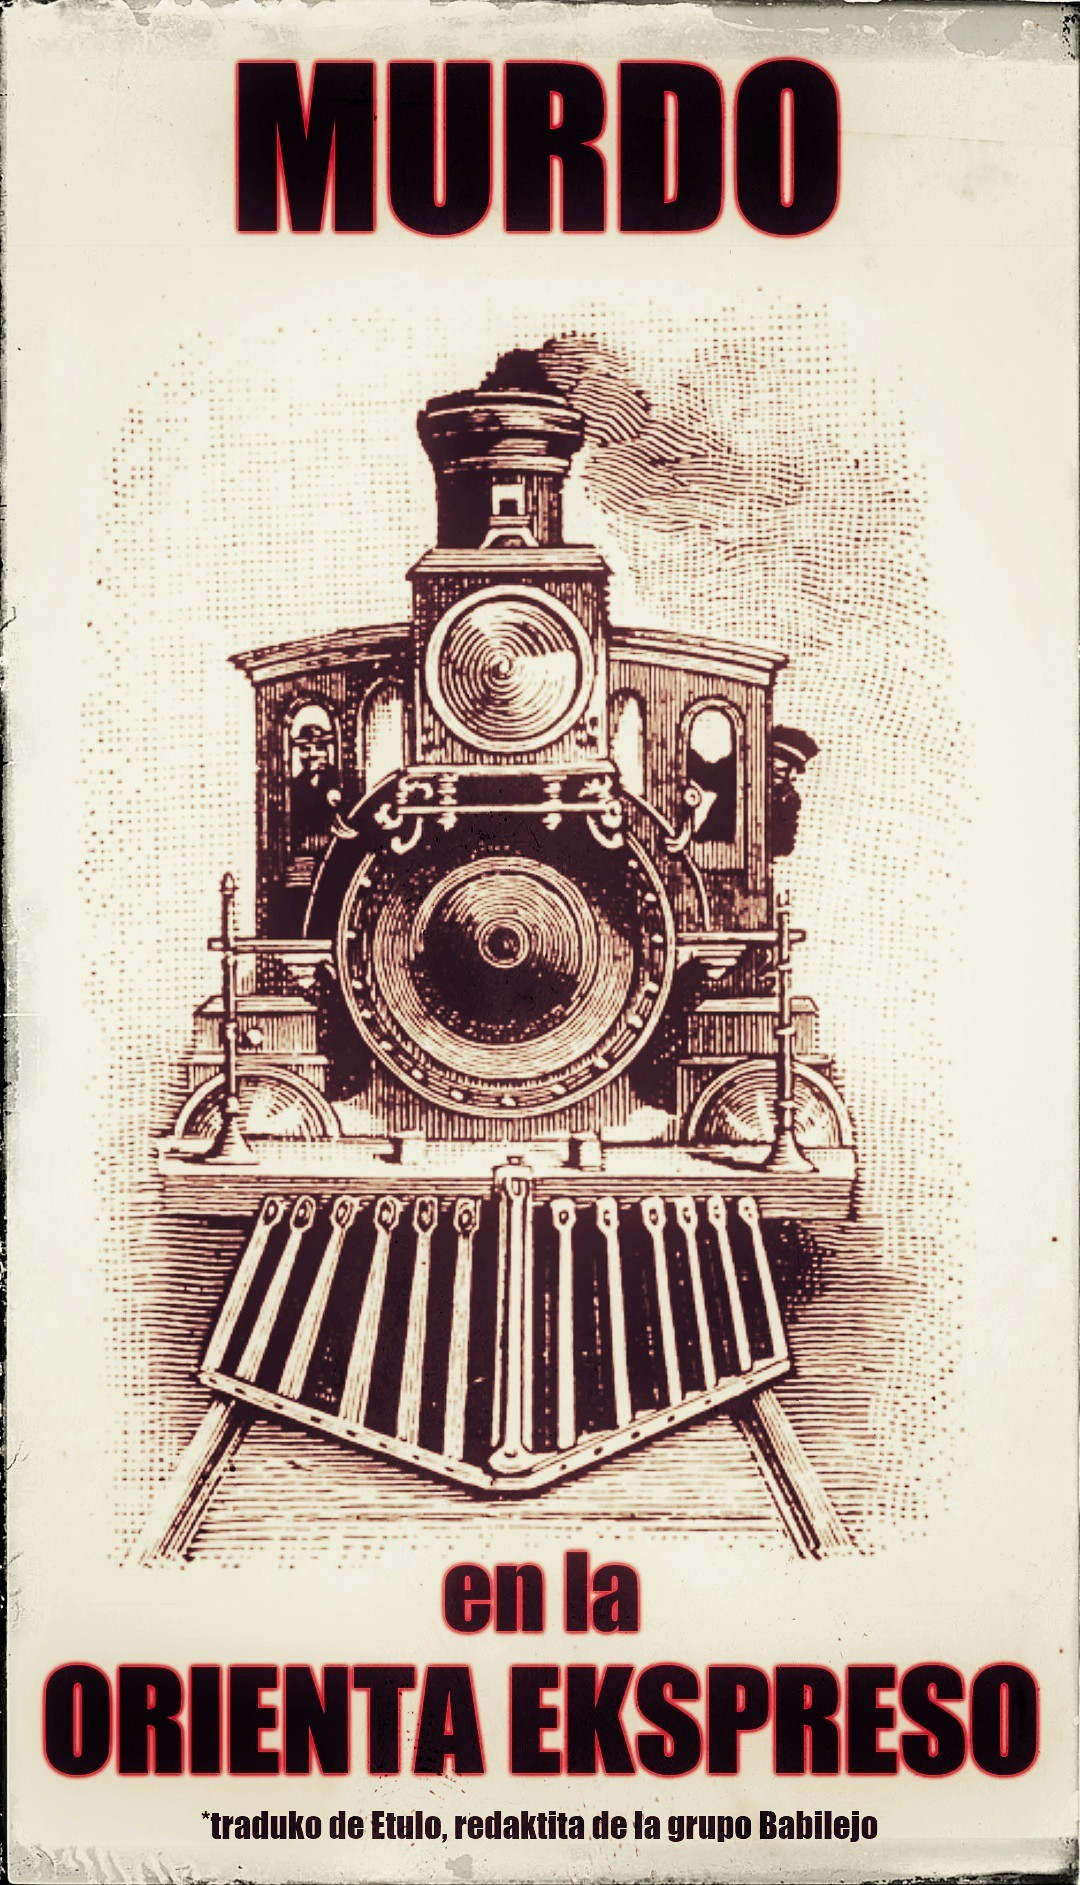
\includegraphics[width=\textwidth,height=\textheight]{cover.jpg} 
	\end{center}
\thispagestyle{empty}
\clearpage
\vspace*{-4em}
\tableofcontents*
\thispagestyle{empty}
\mainmatter
\setcounter{page}{3}

\part{La faktoj}
\renewcommand*{\theHchapter}{chX.\the\value{chapter}}
\setcounter{chapter}{0}


\chapter[Grava pasaĝero en la Taŭruso Expreso]{Grava pasaĝero en la Taŭruso Expreso}


Estis preskaŭ la kvina horo en vintra mateno en Sirio. Apud la kajo en Aleppo estis la trajno pompe nomata en la fervojaj horaroj la Taŭrusa Ekspreso. Ĝi konsistis el manĝ-vagono, dorm-vagono kaj du lokaj vagonoj.

\sectionbreak

Ĉe la ŝtupo de la dorm-vagono staris juna franca leŭtenanto, bele vestita per uniformo, parolanta al malalta viro tiom vestita, ke nenio el li estis videbla escepte de ruĝa nazpinto kaj la du pintoj de liphararo.

Estis glaciige malvarme, kaj tiu deĵoro adiaŭi gravan fremdulon ne estis enviinda, sed Leŭtenanto Dubosc bonhumore faris sian devon. Belsonaj frazoj elvenis el liaj lipoj en eleganta franca lingvo. Tamen, li tute ne sciis pri kio la afero temis. Estis onidiroj, kompreneble, kiel ĉiam estas en tiaj okazoj{\ldots}. La humoro de la generalo --- \emph{lia} generalo --- pli kaj pli malboniĝis. Tiam alvenis ĉi tiu belga fremdulo --- de malproksima Anglujo, ŝajne. Sekvis semajno kurioze streĉa. Poste certaj okazintaĵoj! Tre eminenta oficiro sin mortigis, alia eksiĝis, maltrankvilaj vizaĝoj sereniĝis, certaj armeaj ordonoj nuliĝis. La generalo --- tiu de Leŭtenanto Dubosc --- subite aspektis dek jarojn pli juna.

Dubosc estis aŭdinta parton de interparolado inter li kaj la fremdulo. ``Vi savis nin, \emph{mon cher},'' emocie diris la generalo, ``Vi savis la honoron de la franca armeo --- vi fortenis la elverŝadon de sango! Kiel mi povas danki al vi? Veni tiel malproksimen---''

Al kiu la fremdulo (laŭnome S-ro Hercule Poirot) estis farinta decan respondon, kiu enhavis la frazon, ``Sed ĉu vi ne memoras, ke iam vi savis mian vivon?'' Tiam la generalo faris alian decan respondon, malpretendante ian meriton por tiu ago, kaj post pli da parolado pri Francujo, Belgujo, gloro, honoro, kaj tiaj aferoj ili ĉirkaŭpremis unu la alian kaj la interparolado finiĝis.

Ankoraŭ Leŭtenanto Dubosc ne sciis pri kio ĉio temis, sed al li oni donis la devon adiaŭi S-ron Poirot ĉe la Taŭrusa Ekspreso, kaj li fervore plenumis ĝin kiel estas dece por juna oficiro, kiu havas antaŭ si promesplenan karieron.

``Hodiaŭ estas dimanĉo,'' diris Leŭtenanto Dubosc. ``Morgaŭ, lundo vespere, vi estos en Istanbul.''

Ne estis la unua fojo, ke li tion diris. Konversacioj sur kajo, antaŭ la foriro de trajno, kutime enhavas ripetaĵojn.

``Vi estas prava,'' konsentis S-ro Poirot.

``Kaj vi intencas pasigi kelkajn tagojn tie, ĉu ne?''

``\emph{Mais oui}. Istanbul estas urbo kiun mi neniam vizitis. Estus domaĝe trairi ĝin --- \emph{comme ça}.'' Li esprime klakis per la fingroj.

``Nenio urĝas --- mi restos tie dum kelkaj tagoj kiel turisto.''

``\emph{La Sainte Sophie}, ĝi estas tre bela,'' diris Leŭtenanto Dubosc, kiu ne estis vidinta ĝin.

Malvarma vento blovegis trans la kajo. La du viroj tremis. Leŭtenanto Dubosc sukcesis kaŝe ekrigardi sian horloĝeton. Kvin minutoj antaŭ la kvina --- nur kvin minutojn!

Kredante, ke la alia estis vidinta sian kaŝan ekrigardon, li rapidis paroli denove.

``Malmultaj personoj veturas en la nuna jarperiodo,'' li diris, ekrigardante la fenestrojn de la dorm-vagono super ili.

``Konsentite,'' diris S-ro Poirot.

``Ni esperu, ke vi ne estos neĝblokita en la Taŭrus!''

``Ĉu tio okazas?''

``Jes, ĝi okazis. Ne dum ĉi tiu jaro ĝis nun.''

``Do, ni esperu,'' diris S-ro Poirot.'' La raportoj pri la vetero en Eŭropo estas malbonaj.''

``Tre malbonaj. En la balkanaj regionoj estas multe da neĝo.''

``Ankaŭ en Germanujo, mi informiĝis.''

``\emph{Eh bien},'' diris Leŭtenanto Dubosc rapide, ĉar alia paŭzo ŝajnis ebla.

``Morgaŭ vespere je la sepa kvardek vi estos en Istanbul.''

``Jes,'' diris S-ro Poirot, kaj daŭrigis senespere, ``\emph{La Sainte Sophie}, mi aŭdis, ke ĝi estas tre bela.''

``Grandioza, mi opinias.''

Super iliaj kapoj la kurteno de dorm-kupeo estis forpuŝata kaj fraŭlino ekrigardis.

Mary Debenham malmulton dormis de kiam ŝi forlasis Bagdad la antaŭan ĵaŭdon. Nek en la trajno al Kirkuk, nek en la Ripoza Domo en Mosul, nek la lastan nokton en la trajno ŝi dormis kontentige. Nun, laca pro la sendorma kuŝado en la sufoka aero de sia tro varmigita kupeo, ŝi levis sin kaj elrigardis.

La loko devas esti Aleppo. Nenio vidinda, kompreneble. Nur longa, malbone lumigita kajo kun ie koleraj interparoloj arablingve. Du viroj sub ŝia fenestro parolis france. Unu estis franca oficiro, la alia estis malgranda viro kun grandega liphararo. Ŝi iomete ridetis. Ŝi neniam vidis iun tiom vestita. Devas esti tre malvarme ekstere. Jen kial oni tiom terure varmigis la trajnon. Ŝi provis pli malfermi la fenestron, sed ŝi ne sukcesis.

La Wagon Lit konduktoro venis al la du viroj. La trajno estis ekironta, li diris. Estus bone, ke monsieur eniru. La malgranda viro deprenis sian ĉapelon. Kian ovformatan kapon li havas! Spite siajn ĝenaĵojn Mary Debenham ridetis. Ridige aspekta vireto! La tipo de vireto, kiun oni neniam povas serioze konsideri.

Leŭtenanto Dubosc estis diranta sian adiaŭan parolon. Li estis elpensinta ĝin antaŭe, kaj rezervis ĝin ĝis la lasta minuto. Ĝi estis tre bele konstruita parolo.

Konforme, S-ro Poirot faris elegantan respondon.

``\emph{En voiture, Monsieur},'' diris la konduktoro de la Wagon Lit.

Kun ŝajniga bedaŭro S-ro Poirot eniris la trajnon. La konduktoro eniris post li. S-ro Poirot flirtis la manon. Leŭtenanto Dubosc salutis. La trajno per subita ekmovo malrapide antaŭeniris.

``\emph{Enfin}!'' murmuris S-ro Hercule Poirot.

``\emph{Brrrrr},'' diris Leŭtenanto Dubosc, eksciante kiel malvarma li estas{\ldots}.

\sectionbreak

``\emph{Voilà, Monsieur}.'' La konduktoro montris al Poirot per drama gesto la belecon de lia dorm-kupeo kaj la ordan aranĝon de liaj pakaĵoj.

``La etan valizon de Monsieur, mi metis ĉi tien.''

Lia elmetita mano estis sugesta. Hercule Poirot metis en ĝin monbileton.

``\emph{Merci, Monsieur}.'' La konduktoro iĝis vigla kaj aferema.

``Mi havas la biletojn de Monsieur. Mi petas ankaŭ la pasporton. Monsieur eliros en Istanbul, mi kredas?''

S-ro Poirot konsentis.

``Ne multaj personoj kunveturas, mi supozas?'' li diris.

``Ne, Monsieur. Nur estas du aliaj pasaĝeroj --- ambaŭ angloj. Kolonelo el Hindujo, kaj juna anglino el Bagdad. Ĉu Monsieur bezonas ion?''

Monsieur mendis malgrandan botelon da Perrier.

La kvina matene estas maloportuna horo entrajniĝi. Estis ankoraŭ du horoj antaŭ la sunleviĝo. Konscia pri nesufiĉa dormo, kaj pri malfacila tasko sukcese farita, S-ro Poirot sidiĝis en angulo kaj endormiĝis.

\sectionbreak

Kiam li vekiĝis estis la naŭa kaj duono, kaj li iris al la manĝ-vagono por havigi varman kafon.

Estis nur unu alia ĉeestanto je tiu momento, videble la juna anglino priparolita de la konduktoro. Ŝi estis alta, gracia, kaj malhela, eble dudek-ok jara. En la maniero laŭ kiu ŝi manĝis kaj mendis de la servisto pli da kafo oni povis vidi ke ŝi jam kutimiĝis al vojaĝado. Ŝi portis malhelan robon el maldika ŝtofo tre taŭga pro la varmigita aero en la trajno.

S-ro Hercule Poirot, ne havante ion pli bonan por fari, amuzis sin konsiderante ŝin sen ŝia scio.

Ŝi estis, liaopinie, tia fraŭlino kia povas facile prizorgi sin ie ajn. Ŝi havis ekvilibron kaj kompetentecon. Li iom ŝatis la regulecon de ŝia vizaĝo kaj la delikatan palecon de ŝia haŭto. Li ŝatis la nigran kapon kun ĝiaj ordaj ondoj de la haroj, kaj ŝiajn okulojn, malvarmajn kaj grizajn. Sed ŝi estas, li decidis, iom tro kompetenta por esti tiu, kiun li nomas ``\emph{jolie femme}.''

Baldaŭ envenis en la manĝ-vagonon alia persono. Tiu estis alta viro, kiu havas inter kvardek kaj kvindek jarojn, iom maldika, brunhaŭta, kun la haroj iomete grizaj.

``La Kolonelo el Hindujo,'' diris Poirot al si.

La novalveninto sin klinetis al la fraŭlino.

``Bonan matenon, F-ino Debenham.''

``Bonan matenon, Kolonelo Arbuthnot.''

La Kolonelo estis staranta kun mano sur la seĝo kontraŭ ŝi.

``Ĉu vi permesos?''

``Kompreneble. Sidiĝu.''

``Nu, vi scias, ke la matenmanĝo ne estas ĉiam interparola manĝo.''

``Mi tion esperas. Sed mi ne mordas.''

La kolonelo sidiĝis.

``Kelnero,'' li vokis ordone.

Li mendis kafon kaj ovojn.

Liaj okuloj rigardis momente Hercule Poirot, sed la rigardo forvagis. Poirot, legante ĝuste la anglan menson, sciis ke li diris al si, ``Nur stulta alilandano.''

Laŭ la nacia kutimo, la du angloj ne multe parolis. Ili interŝanĝis kelkajn vortojn, kaj baldaŭ la fraŭlino levis sin kaj reiris al sia kupeo.

Dum la tagmeza manĝo la du denove estis ĉe la sama tablo, kaj denove ili tute ignoris la trian pasaĝeron. Ili parolis pli ol dum la matenmanĝo. Kolonelo Arbuthnot parolis pri la Punjab,\footnote{Provinco en la norda parto de Hindujo.} kaj kelkfoje faris al la fraŭlino demandojn pri Bagdad, kaj evidentiĝis ke ŝi deĵoris tie kiel guvernistino. Dum la interparolo ili eltrovis ke ili havas komunajn amikojn, kaj rezulte ili iĝis pli amikaj. Ili parolis pri Tomaso Iu kaj Jerry Tiu. La kolonelo petis informon ĉu ŝi intencas iri rekte al Anglujo, aŭ ĉu ŝi haltos en Istanbul.

``Ne, mi ne haltos.''

``Ĉu ne domaĝe?''

``Mi venis laŭ ĉi tiu vojo antaŭ du jaroj, kaj tiam pasigis tri tagojn en Istanbul.''

``Mi komprenas. Nu, mi povas diri, ke mi estas tre kontenta ke vi senhalte veturos, ĉar tion mi ankaŭ faros.''

Li mallerte sin klinis, iomete ruĝiĝante.

``Li estas impresebla, nia kolonelo,'' pensis Hercule Poirot amuzata. ``La trajno estas tiom danĝera kiom marvojaĝo.''

F-ino Debenham trankvile diris, ke tio estos agrabla. Ŝia sinteno estis iom malvarma.

Hercule Poirot rimarkis, ke la kolonelo akompanis ŝin al ŝia kupeo. Poste ili preterpasis la belegan pejzaĝon de la Taŭrus. Ili staris flankon ĉe flanko en la koridoro, kaj subite la fraŭlino suspiris. Poirot staris apude, kaj aŭdis ŝin murmuri :

``Ĉio estas tiel bela! Mi volus --- mi volus---''

``Jes?''

``Mi volus, ke mi povu ĝui ĝin!''

Arbuthnot ne respondis. La linio de lia makzelo aspektis iom pli severa.

``Mi tre volas, ke vi estu ekster la afero,'' li diris.

``Silentu, mi petas. Silentu.''

\sectionbreak

``Ho! bone.'' Li iom ĉagrenite ekrigardis S-ron Poirot. Tiam li daŭrigis:

``Sed mi ne ŝatas la ideon, ke vi estas guvernistino --- je ĉiu deziro de tiranaj patrinoj kaj \emph{iliaj} enuigaj infanaĉoj.''

Ŝi ridetis.

``Vi devas ne pensi tion. La subpremita guvernistino estas legendo ne plu vera. Mi povas certigi al vi, ke estas la gepatroj kiuj timas \emph{min}.''

Ili ne plu parolis. Eble Arbuthnot iom hontis pro sia eldiro.

``Iom stranga komedieto kiun mi rigardas,'' pense diris Poirot al si. Poste li memoris tiun penson.

Ili alvenis en Konya tiunokte je la dek-unua kaj duono. La du anglaj vojaĝantoj eliris kaj promenis sur la neĝkovrita kajo.

S-ro Poirot estis kontenta rigardi la movadon en la stacidomo tra fenestro. Tamen, post dek minutoj li decidis, ke iom da freŝa aero estus bona por li. Li zorge pretigis sin, surmetis kelkajn jaketojn kaj koltukojn, kaj metis siajn ŝuojn en galoŝojn. Tiel vestita li malsupreniris al la kajo kaj komencis promeni laŭlonge de ĝi. Li preterpasis la lokomotivon.

Estis la voĉoj, kiuj indikis al li la du malklaraj formoj, kiuj staras en la ombro de vagono. Arbuthnot parolis.

``Mary---''

La fraŭlino interrompis lin.

``Ne nun. Ne nun. Kiam ĝi estos finita. Kiam ĝi estos finita --- \emph{tiam}---''

Diskrete S-ro Poirot forturnis sin. Li miris.

Li preskaŭ ne estus rekoninta la malvarman kompetentan voĉon de F-ino Debenham.

``Kurioze,'' li diris al si.

La postan tagon li scivolis, ĉu eble ili kverelis. Ili malmulte interparolis. La fraŭlino, li pensis, aspektas ĝenata. Estis malhelaj ombroj sub ŝiaj ouloj.

Proksimume je la dua kaj duono posttagmeze la trajno haltis. Kapoj aperis ĉe la fenestroj. Eta aro da viroj estis apud la reloj kaj indikis ion sub la manĝ-vagono.

Poirot metis la kapon eksteren, kaj parolis al la konduktoro de la Wagon Lit, kiu rapide preterpasis. La viro respondis, kaj Poirot sin turnante preskaŭ koliziis kun Mary Debenham, kiu staris tuj malantaŭ li.

``Kio okazis?'' ŝi demandis franclingve. ``Kial ni haltas?''

``Estas nenio, fraŭlino. Io ekbrulis sub la manĝ-vagono. Nenio grava. Ili nun riparas la malbonaĵon. Nenia danĝero, mi certigas al vi.''

Ŝi faris abruptan gesteton, kvazaŭ la ideo de danĝero tute ne gravas al ŝi.

``Jes, jes, tion mi komprenas. Sed la \emph{tempo}!''

``La tempo?''

``Jes, tio malfruigos nin.''

``Estas eble --- jes,'' konsentis Poirot.

``Sed malfruiĝon ni ne povas allasi! La trajno devus alveni je 6.55, kaj oni devas transiri la Bosphorus por trafi la Orientan Ekspreson ĉe la alia flanko je la naŭa. Se estus unu hora malfruiĝo, ni maltrafus tiun trajnon.''

``Estas eble, jes,'' li aprobis.

Li rigardis ŝin scivoleme. La mano, kiu tenis la fenestro-barilon ne estis tute firma, ankaŭ ŝiaj lipoj tremetis.

``Ĉu ĝi estas tre grava al vi, fraŭlino?'' li demandis.

``Jes, tre grava. Mi \emph{devas} trafi tiun trajnon.''

Ŝi forturnis sin, kaj iris laŭ la koridoro al Kolonelo Arbuthnot.

Ŝia maltrankvilo ne necesis. Post dek minutoj la trajno ekveturis, kaj alvenis ĉe Haydapassar nur kvin minutojn malfrue.

La Bosphorus estis maltrankvila kaj S-ro Poirot ne ĝuis la transiron. Li apartiĝis de siaj kunvojaĝantoj sur la ŝipo, kaj ne revidis ilin.

Post alveno ĉe la Ponto Galata li iris rekte al la Hotelo Tokatlian.

\chapter[La hotelo Takatlian]{La hotelo Takatlian}


Ĉe la Tokatlian, Hercule Poirot petis ĉambron kun bano. Tiam li iris al la tablo de la komizo kaj petis siajn leterojn.

Tri leteroj kaj telegramo atendis lin. Liaj brovoj iom leviĝis ĉe vido de la telegramo. Ĝi estis neatendata.

Li malfermis ĝin laŭ sia orda maniero. La presitaj vortoj estis klaraj.

\begin{center}\itshape "Evoluo antaŭvidita de vi en Kassner Afero subite okazis revenu tuj."\end{center}

``\emph{Voilà ce qui est embêtant,}'' murmuris Poirot ĉagrenite. Li ekrigardis la horloĝon.

``Mi devos antaŭeniri hodiaŭ nokte,'' li diris al la komizo.

``Je kioma horo ekveturos la Simplon Orient?''

``Je la naŭa, Monsieur.''

``Ĉu vi povos havigi dorm-kupeon por mi?''

``Certe, Monsieur. Ne estas malfacilaĵo en la nuna sezono. La trajnoj estas preskaŭ malplenaj. Unuaklasa aŭ dua?''

``Unua.''

``\emph{Très bien, Monsieur. Ĝis kie?}''

``Ĝis Londono.''

``\emph{Bien, Monsieur.} Mi havigos bileton por Londono kaj rezervos vian dorm-kupeon en la Istanbul-Calais vagono.''

Poirot denove ekrigardis la horloĝon. Estis dek minutoj antaŭ la oka.

``Mi havas sufiĉe da tempo por manĝi?''

``Sed certe, Monsieur.''

La malgranda belgo kapjesis. Li nuligis sian mendon por ĉambro kaj iris al la manĝejo. Dum li donis sian mendon al kelnero iu metis manon sur lian ŝultron.

``Ho! \emph{Mon vieux}, jen neatendita plezuro,'' diris voĉo malantaŭ li.

La parolinto estis malalta, dika, nejuna viro, kun la hararo tranĉita \emph{en brosse}. Li kontente ridetis.

Poirot eksaltis.

``Monsieur Bouc.''

``Monsieur Poirot.''

M. Bouc estis belgo, direktoro de la Compagnie Internationale des Wagon Lits, kaj li konis la antaŭan stelon de la belga policaro jam dum multaj jaroj.

``Vi estas malproksime de la hejmo, mon cher,'' diris M. Bouc.

``Io okazis en Sirio.''

``Do! Kaj vi reiras hejmen --- kiam?''

``Hodiaŭ vespere.''

``Bonega! Mi ankaŭ. Tio estas, mi iros ĝis Lausanne, kie aferoj atendas min. Vi veturos per la Simplon Orient, ĉu ne?''

``Jes. Mi ĵus petis, ke oni havigu dorm-kupeon por mi. Mi intencis resti ĉi tie kelkajn tagojn, sed mi ricevis telegramon, kiu revokas min al Anglujo.''

``Do!'' suspiris M. Bouc. ``\emph{Les affaires --- les affaires!} Sed vi --- vi estas gravulo nun, \emph{mon vieux}!''

``Eble mi havis iomete da sukceso.'' Hercule Poirot provis aspekti iom modesta, sed tute malsukcesis.

Bouc ridis.

``Ni renkontiĝos poste,'' li diris.

Hercule Poirot daŭrigis la taskon teni siajn lipharojn el la supo. Tiun malfacilan taskon plenuminte, li ĉirkaŭrigardis atendante la venontan pladon. Estis nur proksimume ses personoj en la restoracio, kaj el tiuj nur du interesis Hercule Poirot.

Ili sidis ĉe proksima tablo. La pli juna estis afable aspekta junulo tridekjara, videble usonano. Tamen ne estis li sed lia kunulo, kiu altiris la atenton de la malalta detektivo.

Li estis viro inter sesdekjara kaj sepdekjara. De malproksime li havis la aspekton de filantropo. Lia iom senhara kapo, lia granda frunto, la ridetanta buŝo, kiu montris tre blankan dentaron, ĉiuj ŝajnis aparteni al donacema persono. Nur la okuloj neis tiun impreson. Ili estis malgrandaj, enkaviĝintaj, kaj ruzaj. Ne nur tio. Kiam la viro, parolante al sia juna kunulo, ekrigardis trans la ĉambron, lia rigardo restis dum momento ĉe Poirot, kaj dum tiu sekundo estis stranga malamo en liaj okuloj.

Li ekleviĝis.

``Pagu la kalkulon, Hector,'' li diris.

Lia voĉo estis iom raŭketa. Ĝi havis strangan, molan, danĝeran econ.

Kiam Poirot rekuniĝis kun sia amiko en la ripozejo, la aliaj du viroj estis forlasantaj la hotelon. La pli juna prizorgis la forprenon de la pakaĵoj. Baldaŭ poste li malfermis la vitran pordon, kaj diris:

``Tute preta nun, S-ro Ratchett.''

La pli maljuna viro jesis kaj eliris.

``\emph{Eh bien},'' diris Poirot.

``Kion vi opinias pri tiuj du?''

``Ili estas usonanoj,'' diris M. Bouc.

``Sendube ili estas usonanoj. Mi intencis diri, kion vi opinias pri iliaj personecoj?''

``La junulo ŝajnis esti afabla.''

``Kaj la alia?''

``Verdire, mia amiko, mi ne ŝatis lin. Li donis al mi malbonan impreson. Kaj vi?''

Hercule Poirot ne respondis dum momento.

``Kiam li pasis min en la restoracio, mi ricevis strangan impreson,'' li diris. ``Estis kvazaŭ sovaĝa besto --- besto furioza --- pasis min.''

``Tamen li aspektis tute respektinda.''

``Precize! La korpo --- la korpo --- estas tute respektinda --- sed tra la bariloj elrigardas la sovaĝa besto.''

``Vi estas fantazia, \emph{mon vieux},'' diris M. Bouc.

``Povas esti. Sed mi ne povis forigi la impreson, ke io malbona pasis min tute proksime.''

``Tiu respektinda usonano?''

``Tiu respektinda usonano!''

``Nu,'' diris M. Bouc gaje. ``Povas esti. Estas multe da malbono en la mondo.''

Tiumomente la pordo malfermiĝis kaj la komizo alproksimiĝis. Li aspektis ĝenata kaj pardonpetema.

``Estas eksterordinare, Monsieur,'' li diris al Poirot.

``Ne estas eĉ unu unuaklasa dorm-kupeo libera en la trajno.''

``\emph{Comment}?'' diris M. Bouc. ``Je tiu jartempo? Sendube estas aro da ĵurnalistoj --- da politikistoj---?''

``Mi ne scias, sinjoro,'' respondis la komizo ĝentile. ``Sed estas tiel.''

``Nu,'' M. Bouc turnis sin al Poirot. ''Ne timu, mia

amiko. Ni aranĝos ion. Ĉiam estas unu kupeo --- n-ro 16, kiu ne estas rezervita. La konduktoro tion prizorgas!'' Li ridetis, tiam ekrigardis la horloĝon. ``Venu, ni devas ekiri.''

Ĉe la stacidomo la brun-vestita konduktoro de la Wagon-Lit tre ĝentile salutis M. Bouc.

``Bonan vesperon, sinjoro. Via kupeo estas n-ro 1.''

Li alvokis la portistojn kaj ili prenis la pakaĵojn laŭlonge de la vagono sur kiu la indikiloj montris ĝian celatan lokon:

\begin{center}{ISTANBUL TRIESTE CALAIS\\}\end{center}

``Vi estas tute plena hodiaŭ, mi aŭdis?''

``Estas nekompreneble, sinjoro. La tuta mondo decidis veturi hodiaŭ.''

``Ĉiukaze vi devas trovi lokon par ĉi tiu sinjoro. Li estas amiko mia. Li povas havi n-ron 16.''

``Ĝi estas luita, sinjoro.''

``Kio? N-ro 16?''

Ekrigardo kompreniga pasis inter ili, kaj la konduktoro ridetis. Li estis alta, palvizaĝa, mezaĝa viro.

``Sed jes, sinjoro. Kiel mi diris, ni estas tute plenaj --- ĉie.''

``Sed kio okazas?'' kolere demandis M. Bouc. ``Estas konferenco ie? Ĉu ĝi estas kunularo?''

``Ne, sinjoro. Estas nur hazardo. Tiel okazis, ke multaj personoj decidis veturi hodiaŭ nokte.''

M. Bouc faris sonon de ĉagreno.

``En Beograd,'' li diris, ``estos la apartiĝa vagono el Ateno. Estos ankaŭ la Bukarest-Pariza vagono --- sed ni ne atingos Beograd ĝis morgaŭ vespere. La problemo estas la hodiaŭa nokto. Ĉu ne estas dua-klasa kupeo libera?''

``Estas dua-klasa kupeo, sinjoro---''

``Nu, do---''

``Sed ĝi estas por sinjorino. Jam estas germanino en la kupeo --- sinjorina servistino.''

``\emph{Là, là,} tio estas embarasa,'' diris M. Bouc.

``Ne ĝenu vin, mia amiko,'' diris Poirot. ``Mi devas veturi en ordinara vagono.''

``Tute ne. Tute ne.'' Li turnis sin denove al la konduktoro.'' Ĉu ĉiu jam alvenis?''

``Estas vere,'' diris la viro, '' ke unu pasaĝero ĝis nun ne alvenis.''

Li parolis malrapide, heziteme.

``Sed parolu?''

``Lito n-ro 7 --- dua-klasa. La sinjoro ankoraŭ ne alvenis, kaj estas kvar minutoj antaŭ la naŭa.''

``Kiu li estas?''

``Anglo,'' la konduktoro rigardis sian liston. ``Iu sinjoro Harris.''

``Nomo bonaŭgura,'' diris Poirot. ``Mi legas Dickens. S-ro Harris, li ne alvenos.''

``Metu la pakaĵojn en n-ro 7,'' diris M. Bouc. ``Se tiu S-ro Harris alvenus, mi diros al li ke li estas tro malfrua --- ke ni ne povas tiel longe rezervi litojn --- ni iamaniere aranĝos la aferon. Kial mi ĝenu min pri iu S-ro Harris?''

``Laŭ via deziro,'' diris la konduktoro.

Li parolis al la portisto de Poirot, kaj indikis kien li iru. Tiam li flanken staris por ke Poirot eniru la trajnon.

``\emph{Tout à fait au bout, Monsieur,}'' li vokis. ``La antaŭlasta kupeo.''

Poirot trapasis la koridoron, iom malrapide, ĉar preskaŭ ĉiu staris ekster sia kupeo. Tute regule, li ĝentile diris ``\emph{Pardon}.'' Fine li atingis la indikitan kupeon. En ĝi estis la alta juna usonano de la Hotelo Tokatlian. Li sulkigis la brovojn ĉe la eniro de Poirot.

``Pardonu al mi,'' li diris. ``Mi opinias, ke vi faris eraron.'' Tiam, malrapide en franca lingvo, ``\emph{Je crois que vous avez un erreur.}''

Poirot respondis anglalingve.

``Vi estas s-ro Harris?''

``Ne, mia nomo estas MacQueen. Mi---''

Sed je tiu momento la voĉo de la konduktoro sonis super la ŝultro de Poirot. Senkulpiga, iom senspira voĉo.

``Ne estas alia kupeo en la vagonaro, sinjoro. La sinjoro devas veni ĉi tien.'' Samtempe li komencis enmeti la pakaĵojn.

Poirot rimarkis la senkulpigan voĉtonon kun iom da amuzo. Sendube la alia veturanto estis promesinta al li bonan trinkmonon por la sola uzo de la kupeo. Tamen eĉ la plej granda trinkmono nenion valoras kiam direktoro de la fervojo ĉeestas kaj faras ordonon.

La konduktoro metis la pakaĵojn sur la pakaĵ-breton kaj elvenis el la kupeo.

``\emph{Voilà, Monsieur,}'' li diris. ``Ĉio estas preta. La supera lito estas via, la numero 7. Ni ekveturas post unu minuto.''

Li forrapidis tra la koridoro. Poirot reeniris la kupeon.

``Okazintaĵo, kiun mi malofte vidis,'' li diris gaje. ``Wagon Lit konduktoro mem metas la pakaĵojn! Nekutimaĵo!''

Lia kunveturanto ridetis. Evidente la afero ne plu ĝenis lin --- kredeble li estis decidinta akcepti ĝin filozofe.

``La trajno estas nekutime plena,'' li diris.

Eksonis fajfilo, estis longa, melankolia krio de la lokomotivo. La du viroj iris en la koridoron.

Ekstere voĉo kriis, ``\emph{En voiture.}''

``Ni ekveturas,'' diris MacQueen.

Sed ne tute. La fajfilo ree sonis.

``Nu, sinjoro,'' subite diris la junulo, ``se vi preferus la suban liton mi estus tute kontenta.''

Ŝatinda junulo.

``Ne, ne,'' protestis Poirot. ``Mi ne deziras ĝeni vin---''

``Estas tute bone---''

``Vi estas tro afabla---''

Ĝentilaj protestoj ambaŭflanke.

``Estas nur dum unu nokto,'' klarigis Poirot. ``Ĉe Beograd---''

``Nu, mi komprenas. Vi eliros en Beograd---''

``Ne precize. La fakto estas---''

Estis subita ekmovo. Ambaŭ viroj turnis sin al la fenestro, kaj rigardis la longan lumigitan kajon kiu malrapide preterpasis ilin. La Orienta Ekspreso komencis sian tri-tagan vojaĝon trans Eŭropo.

\chapter[Poirot malakceptas proponon]{Poirot malakceptas proponon}


M. Hercule Poirot iomete malfruis kiam li eniris la manĝ-vagonon la sekvantan tagon. Li estis ellitiĝinta frue, matenmanĝinta preskaŭ sole, kaj pasiginta la matenon konsiderante la notojn pri la afero, kiu vokis lin al Londono. Li estis vidinta malofte sian kunveturanton.

M. Bouc, kiu jam sidiĝis, gestis saluton, kaj vokis sian amikon al la libera loko kontraŭ li. Poirot sidiĝis kaj baldaŭ trovis ke lia tablo estas la unua, kiu ricevas atenton kaj la plej bonajn manĝaĵojn.

Estis nur kiam ili manĝas bongustan krem-fromaĝon, ke M. Bouc permesis sin pensi pri aliaj aferoj. Li estis je tiu periodo de manĝo, kiam oni estiĝas filozofa.

``Nu!'' li diris. ``Se mi nur havus la plumon de Balzac! Mi priskribus ĉi tiun lokon.''

Li mangestis.

``Bona ideo, tio,'' diris Poirot.

``Vi konsentas? Oni ne faris ĝin, miaopinie? Tamen ĝi estas romaneca. Ĉirkaŭ ni estas personoj el ĉiuj klasoj, el ĉiuj nacioj, el ĉiuj aĝoj. Dum tri tagoj ĉi tiuj personoj, fremdaj unu al la aliaj, estas kune. Ili manĝas kaj dormas sub unu plafono, ili ne povas disiĝi. Post tiuj tri tagoj ili apartiĝos, ili iros laŭ siaj propraj deziroj, kaj kredeble neniam revidos unu la alian.''

``Tamen,'' diris Poirot, '' supozu, ke akcidento---''

``Ne, ne, mia amiko---''

``De via vidpunkto tio estus bedaŭrindaĵo, mi konsentas. Tamen, supozu tion dum momento. Eble tiuokaze, ĉiuj ĉi tie estus kunligitaj --- per la morto.''

``Pli da vino,'' diris M. Bouc, rapide elverŝante ĝin. ``Vi estas malgaja, \emph{mon cher}. Eble pro la digesto.''

``Estas vere,'' konsentis Poirot, ``ke la manĝaĵoj en Sirio eble ne taŭgis por mia stomako.''

Li trinketis sian vinon. Tiam lia rigardo penseme vagadis ĉirkaŭ la manĝ-vagono. Estis dek tri personoj, kaj, kiel diris M. Bouc, el ĉiuj klasoj kaj nacioj. Li komencis studi ilin.

Ĉe la tablo kontraŭ ili estis tri viroj. Ili estas, li supozis, unuopaj veturantoj kune metitaj laŭ la decido de la servistoj. Granda malpala italo kontente pikis la dentojn. Kontraŭ li maldika, bonorda anglo portis la senespriman vizaĝon de la bone-instruita servisto. Apud li estis granda usonano en brilaĉa kompleto --- eble komerca vojaĝanto.

``Vi devas troigi ĝin,'' li estis diranta per laŭta naza voĉo.

La italo forprenis la dent-pikilon por gesti per ĝi.

``Prave,'' li diris.

``Jen kion mi ĉiam diras.''

La anglo rigardis el la fenestro, kaj tusis.

La rigardo de Poirot pluen vagis.

Ĉe malgranda tablo estis unu el la plej malbelaj virinoj, kiun li iam vidis. Ĝi estis malbeleco distinga --- ĝi ĉarmis pli ol forpelis. Ŝi sidis tre rekte. Ĉirkaŭ ŝia kolo estis kolumo el tre grandaj perloj. Ŝiaj manoj estis kovritaj da ringoj. Ŝia zibela palto estis sur ŝiaj ŝultroj. Malgranda multekosta ĉapelo ne plibeligis la flavan, bufaspektan vizaĝon sub ĝi.

Ŝi estis parolanta al la servisto per klara, ĝentila, sed tute aŭtokrata tono.

``Vi kompleze metos en mian kupeon botelon da mineralakvo kaj grandan glason da oranĝsuko. Vi aranĝos, ke mi ricevu ĉe la hodiaŭa vespermanĝo kokidon kuiritan sen saŭcoj --- ankaŭ iom da bolita fiŝo.''

La servisto ĝentile respondis, ke li tion faros.

Ŝi gracie kapjesis kaj ekstaris. Ŝi ekvidis Poirot, kaj rigardis lin laŭ la indiferenteco de neinteresita aristokrato.

``Tiu estas Princino Dragomiroff,'' mallaŭte diris S-ro Bouc. ``Ŝi estas rusino. Ŝia edzo enmonigis sian tutan posedaĵon antaŭ la revolucio, kaj investis ĝin en aliaj landoj. Ŝi estas tre riĉa. Kosmopolitino.''

Poirot kapjesis. Li jam aŭdis pri Princino Dragomiroff. ``Ŝi estas elstara persono,'' diris S-ro Bouc. ``Tiel malbela kiel la peko, sed ŝi rimarkigas sin. Vi konsentas?''

Poirot konsentis.

Ĉe alia el la grandaj tabloj Mary Debenham sidis kun du aliaj virinoj. Unu estis alta mezaĝa virino en bluzo kaj jupo. Ŝi havis amason da velkitaj flavaj haroj malbele aranĝitaj, portis okulvitrojn, kaj havis longan, afablan vizaĝon iom kiel ŝafo. Ŝi aŭskultis la trian virinon, dika, iom maljuna virino kun agrabla vizaĝo, kiu parolis per malrapida, klara unutona voĉo, kiu montris nenian signon ke ĝi volis halti. ``{\ldots}Kaj tial mia filino diris `Ne estas eble, ke vi apliku usonajn metodojn en ĉi tiu lando. La homoj ĉi tie estas nature malenergiaj,' ŝi diris. `Ili tute ne posedas energion.' Malgraŭ tio, surprizus vin scii kion faras nia kolegio tie. Ĝi akiris bonegan instruistaron. Miaopinie, estas nenio tiel grava kiel la eduko. Ni devas apliki niajn okcidentajn idealojn, kaj instrui la orienton rekoni ilin. Mia filino diras---''

La trajno eniris tunelon. La trankvila unutona voĉo droniĝis.

Ĉe la apuda malgranda tablo sidis Kolonelo Arbuthnot --- sola. Li fikse rigardis la kapon de Mary Debenham. Ili ne sidis kune, kvankam ili povus facile tion aranĝi. Kial?

Eble, pensis Poirot, Mary Debenham ne konsentis. Guvernistino lernas esti zorgema. Ŝajnaĵoj estas gravaj. Fraŭlino, kiu devas akiri la vivrimedon devas esti diskreta.

Lia rigardo vagis al la alia flanko de la vagono. Ĉe la fino estis mezaĝa virino, nigre-vestita, kun larĝa senesprima vizaĝo. Germanino aŭ Skandinavino, li pensis. Kredeble germana sinjorina servistino.

Apud ŝi estis paro, kiu kliniĝis antaŭen kaj rapide interparolis. La viro portis anglajn vestojn --- sed li ne estis anglo. Kvankam Poirot povis vidi nur la malantaŭan parton de lia kapo, ĝia formo kaj la ŝultroj perfidis lin. Granda viro, bonaspekta. Li subite turnis la kapon, kaj Poirot vidis la vizaĝon. Tre bela viro, eble tridekjara, kun hela liphararo.

La virino kontraŭ li estis nur juna --- eble dudekjara. Ŝi portis nigran jaketon kaj jupon, blankan atlasan bluzon, etan ĉapelon laŭmode nerekte surmetita. Ŝi havis belan, fremdaspektan vizaĝon, tute blankan haŭton, grandajn brunajn okulojn, harojn gagatnigrajn. Ŝi fumis cigaredon en longa ingo. La manoj finiĝis per ruĝaj fingro-ungoj. Ŝi portis unu grandan smeraldon fiksita en plateno. Estis koketado en ŝia rigardo kaj voĉo.

``\emph{Elle est jolie --- et chic,}'' murmuris Poirot. ``Edzo kaj edzino --- ĉu?''

S-ro Bouc kapjesis.

``El la hungara ambasadorejo, mi opinias,'' li diris. ``Belega paro.''

Nur estis du aliaj manĝantoj --- MacQueen, la kunveturanto de Poirot, kaj lia dunganto S-ro Ratchett. La lasta frontis kontraŭ Poirot, kaj la duan fojon Poirot zorge rigardis tiun malallogan vizaĝon, kaj rimarkis la falsan bonvolon de la frunto kaj la malgrandajn, kruelajn okulojn.

Sendube S-ro Bouc vidis ŝanĝon en la esprimo de sia amiko.

``Vi rigardas vian sovaĝan beston, ĉu ne?'' li demandis.

Poirot kapjesis. Kiam oni portis al li la kafon, S-ro Bouc ekstaris. Komencinte antaŭ ol Poirot, li estis fininta antaŭ iom da tempo.

``Mi reiras al mia kupeo,'' li diris. ``Venu baldaŭ kaj parolu kun mi.''

``Kun plezuro.''

Poirot trinketis sian kafon kaj mendis likvoron. La servisto iris de tablo al tablo kun sia monskatolo, ricevante pagojn. La voĉo de la maljuna usonanino aŭdiĝis, akra kaj plenda.

``Mia filino diris, `Akiru libreton da manĝ-biletoj kaj vi ne havos ĝenaĵojn.' Nu, tio ne estas vera. Ŝajne ili devas havi dek procentan trinkmonon, kaj mi devas alpagi tiun botelon da mineral-akvo --- aĉa ĝi estis. Ili ne havis Evian aŭ Vichy, kio ŝajnas strange al mi.''

``Tio estas --- ili devas doni la akvon de la lando,'' klarigis la ŝaf-vizaĝa virino.

``Tamen, ŝajnas strange al mi.'' Ŝi malkontente rigardis amaseton de etaj moneroj sur la tablo. ``Rigardu tion, kion li donis al mi. Dinaroj aŭ io. Ĝi aspektas kiel rubaĵo. Mia filino diris---''

Mary Debenham forpuŝis sian seĝon kaj foriris. Kolonelo Arbuthnot ekstaris kaj sekvis ŝin. Kolektinte sian monon, la usonanino same faris, sekvate de la alia sinjorino. La hungaroj jam estis for. En la manĝ-vagono nur restis Poirot kaj Ratchett kaj MacQueen.

Ratchett parolis al sia kunulo, kiu ekstaris kaj foriris. Tiam li mem ekstaris, sed anstataŭ sekvi MacQueen li neatendite sidis sin en la seĝo kontraŭ Poirot.

``Ĉu vi povas afable doni al mi alumeton?'' li diris. Lia voĉo estis mola. ``Mia nomo estas Ratchett.''

Poirot iomete sin klinis. Li metis la manon en sian poŝon kaj eltiris alumetujon, kiun li donis al la alia viro, kiu prenis ĝin sed ne bruligis alumeton.

``Mi opinias,'' li daŭrigis, ``ke mi havas la plezuron paroli al S-ro Hercule Poirot, ĉu ne?''

Poirot denove sin klinis.

``Vi estas prava, Monsieur.''

La detektivo konsciiĝis pri la studa rigardo de tiuj strangaj sagacaj okuloj antaŭ ol la alia denove parolis.

``En mia lando,'' li diris, ``ni senprokraste esprimas niajn celojn. S-ro Poirot, mi deziras ke vi faru ion por mi.''

La brovoj de Hercule Poirot iomete leviĝis.

``Mia klientaro, Monsieur, estas nuntempe limigita. Mi akceptas malmultajn proponojn.''

``Certe, mi komprenas tion. Sed la nuna afero, S-ro Poirot, signifas multan monon.'' Per sia mola persvada voĉo li ripetis la vortojn, ``Multan monon.''

Hercule Poirot silentis dum momento, kaj poste diris, ``Kion vi deziras ke mi faru por vi, Monsieur Ratchett?''

``S-ro Poirot, mi estas riĉulo --- tre riĉa viro. Tiaj viroj havas malamikojn. Mi havas malamikon.''

``Nur unu malamikon?''

``Kion signifas tiu demando?'' rapide demandis Ratchett.

``Monsieur, laŭ mia sperto, kiam viro havas, kiel vi diras, malamikojn, kutime tio signifas ne nur unu malamikon.''

Ratchett ŝajnis esti kontenta pri la respondo de Poirot. Li tuj diris. ``Jes, mi tion komprenas. Malamiko aŭ malamikoj --- ne gravas. Kio gravas estas mia sekureco.''

``Sekureco?''

``Mia vivo estas minacita, S-ro Poirot. Nu, mi estas viro kiu povas prizorgi sin.'' El la poŝo de lia jaketo lia mano montris revolveron dum momento. Li daŭrigis severe, ``Mi opinias, ke mi ne estas viro subite trafebla. Sed miaopinie estus bone duoble certigi certecon. Mi kredas, ke vi estas la viro por gajni mian monon, S-ro Poirot. Kaj memoru --- multan monon.''

Poirot pense rigardis lin dum kelkaj minutoj. Lia vizaĝo estis tute senesprima. La alia povus havi nenian ideon pri liaj pensoj.

``Mi bedaŭras, Monsieur,'' li fine diris. ``Mi ne povas komplezi vin.''

La alia sagace rigardis lin.

``Nomu la pagon deziratan,'' li diris.

Poirot kapneis. ``Vi ne komprenas, Monsieur. Mi estis tre bonŝanca en mia profesio. Mi perlaboris sufiĉe da mono por kontentigi miajn bezonojn kaj miajn dezirojn. Mi nun akceptas nur tiujn proponojn, kiuj interesas min.''

``Vi havas multan aplombon,'' diris Ratchett. ``Ĉu dudek mil dolaroj tentos vin?''

``Certe ne.''

``Se vi eltenas por ricevi pli, vi ne sukcesos. Mi scias kiom valoras io al mi.''

``Ankaŭ mi, Monsieur Ratchett.''

``Kio ne taŭgas pri mia propono?''

Poirot levis sin. ``Se vi pardonos al mi la personaĵon --- via vizaĝo ne plaĉas al mi, Monsieur Ratchett,'' li diris.

Kaj post tio li forlasis la manĝ-vagonon.

\chapter[Ekkrio en la nokto]{Ekkrio en la nokto}


La Simplon Orienta Ekspreso alvenis ĉe Beograd kvaronon antaŭ la naŭa tiuvespere. Ĉar ĝi ne foriros ĝis la 9.15 Poirot malsupreniris al la kajo. Li ne restis longan tempon. Estis malvarmege, kaj ekstere neĝis. Li reiris al sia kupeo. La konduktoro, kiu estis sur la kajo, parolis al li.

``Viaj valizoj estas movitaj, Monsieur, al la kupeo N-ro 1, la kupeo de S-ro Bouc.''

``Kie do estas Sinjoro Bouc?''

``Li movis sin en la vagonon el Ateno, kiun oni ĵus alfiksis.''

Poirot sercis sian amikon. S-ro Bouc ne volis akcepti liajn protestojn.

``Tio estas nenio. Estas pli bone tiel. Vi iras rekte al Anglujo, tial estas pli bone ke vi estu en la traira vagono al Calais. Mi estas tute kontenta ĉi tie. Ĝi estas tute trankvila. Ĉi tiu vagono estas okupata nur de mi kaj greka kuracisto. Sed, mia amiko, kia nokto! Oni diras, ke ne estis tiom da neĝo dum multaj jaroj. Ni esperu, ke ĝi ne atendigos nin. Mi ne estas tro feliĉa tiurilate, mi certigas al vi.''

Akurate je 9.15 la trajno ekiris el la stacidomo. Baldaŭ poste Poirot ekstaris, diris bonan nokton al sia amiko, kaj iris laŭlonge de la koridoro al sia propra vagono, kiu estas en la antaŭa parto apud la manĝ-vagono.

Dum tiu, la dua tago de la vojaĝo, baroj sindetenaj iom malaperis. Kolonelo Arbuthnot staris ĉe la pordo de la kupeo de MacQueen kaj parolis al li.

MacQueen ĉesis paroli kiam li vidis Poirot. Li aspektis surprizita.

``Nu,'' li diris, ``mi opiniis, ke vi forlasis nin. Vi diris, ke vi intencas eltrajniĝi en Beograd.''

``Vi miskomprenis min,'' diris Poirot ridetante. ``Mi memoras nun, ke la trajno ekveturis el Istanbul en la momento kiam ni parolis pri ĝi.''

``Sed viaj pakaĵoj --- ili estas for.''

``Oni movis ilin en alian kupeon --- nur tion.''

``Do, mi komprenas.''

Li rekomencis sian konversacion kun Arbuthnot, kaj Poirot iris laŭlonge de la koridoro.

Du pordojn for de lia kupeo, la maljuna usonanino, S-ino Hubbard, staris parolante al la ŝaf-simila svedino. S-ino Hubbard proponis revuon al ŝi.

``Prenu ĝin, mia kara,'' ŝi diris, ``Mi havas multon por legi. La malvarmeco estas terura, ĉu ne?'' Ŝi amike kapklinis al Poirot.

``Vi estas plej afabla,'' diris la svedino.

``Tute ne. Mi esperas, ke vi bone dormos, kaj ke via kapdoloro estos for en la mateno.''

``Estas nur la malvarmeco. Mi pretigos tason da teo.''

``Ĉu vi havas aspirinon? Tute certe? Mi havas multon. Do, bonan nokton, mia kara.''

Ŝi turnis sin al Poirot, kaj la alia virino foriris.

``Kompatindulino, ŝi estas sveda. Tiom, kiom mi eltrovis, ŝi estas misiistino --- kaj instruas. Afabla, sed ne bone parolas angle. Ŝi estis tiom interesata pri tio, kion mi diris al ŝi pri mia filino.''

Poirot jam sciis ĉion pri la filino de S-ino Hubbard. Ĉiu, kiu komprenas la anglan lingvon, sciis, ke ŝi kaj ŝia edzo estas membroj de la stabo de granda usona kolegio en Smyrna, ke S-ino Hubbard faras sian unuan vojaĝon al la Oriento, kaj kion ŝi opinias pri la turkoj kaj iliaj malprecizaj kutimoj kaj la kondiĉo de iliaj vojoj.

La pordo apud ili malfermiĝis, kaj la maldika, pala servisto elvenis. Poirot ekvidis S-ron Ratchett, kiu sidas en la lito. Li vidis Poirot kaj lia mieno ŝanĝiĝis, malheliĝante pro kolero. Tiam la pordo fermiĝis.

S-ino Hubbard flankentiris Poirot. ``Sciu, ke mi estas morte tima pro tiu viro. Ne la servisto --- la alia --- la mastro. Estas io \emph{malĝusta} rilate al tiu viro. Mia filino diras, ke mi estas tre intuicia. `Kiam la patrino ricevas impreson, ŝi tute pravas,' jen kion diras mia filino. Kaj mi havas impreson pri tiu viro. Li estas en la apuda kupeo, kaj mi ne estas kontenta. Mi metis miajn pakaĵojn antaŭ la traira pordo hieraŭ nokte. Mi pensis, ke mi aŭdis lin ĉe la tenilo. Tute ne surprizus min scii ke tiu viro estas murdisto --- unu el tiuj trajn-rabistoj pri kiuj oni legas. Eble mi estas malsaĝa, sed estas tiel. Mi timas lin. Mia filino diris, ke mi havus facilan vojaĝon, sed iel mi ne estas feliĉa. Eble malsaĝe, mi havas la senton ke io okazos. Kaj kiel tiu afabla junulo povas akcepti esti lia sekretario, mi ne povas kompreni.''

Kolonelo Arbuthnot kaj MacQueen alproksimiĝis al ili laŭ la koridoro.

``Venu en mian kupeon,'' MacQueen diris. ``Ĝis nun ĝi ne estas pretigita por la nokto. Kion mi deziras kompreni pri via politiko en Hindujo estas---''

La du viroj preterpasis ilin kaj daŭrigis laŭ la koridoro al la kupeo de MacQueen.

S-ino Hubbard diris bonan nokton al Poirot. ``Mi intencas enlitiĝi kaj legi,'' ŝi diris. ``Bonan nokton.''

Poirot eniris sian kupeon, kiu estis post tiu de Ratchett. Li enlitiĝis, legis dum duonhoro, kaj tiam forigis la lumon.

\sectionbreak

Li subite vekiĝis post kelkaj horoj. Li sciis, kio vekis lin --- laŭta ĝemo, preskaŭ ekkrio, ie apude. Je la sama momento okazis sono de sonorilo.

Poirot leviĝis kaj lumigis la kupeon. Li rimarkis, ke la trajno staras senmova --- supozeble ĉe stacio.

Tiu ekkrio estis surprizinta lin. Li memoris, ke estas Ratchett en la apuda kupeo. Li malfermis la pordon ĵus kiam la konduktoro de la Wagon Lit alvenis kaj frapis ĉe la pordo de Ratchett. Poirot rigardis tra la iomete malfermita pordo. La konduktoro duan fojon frapis. Sonorilo eksonis, kaj lumo montriĝis super alia pordo. La konduktoro ekrigardis super sia ŝultro.

En la sama momento voĉo el la apuda kupeo aŭdiĝis:

``\emph{Ce n'est rien. Je me suis trompé}.''

``\emph{Bien Monsieur.}'' La konduktoro forrapidis, kaj frapis ĉe la pordo kie estas la lumo.

Poirot ree enlitiĝis, sia menso trankviligita, kaj forigis la lumon. Li rigardis sian horloĝeton. Estis precize dudek-tri minutoj antaŭ la unua.

\chapter[La krimo]{La krimo}


Estis malfacile tuj endormiĝi. Li sentis la mankon de la trajn-movo. Se ĝi estis ĉe stacio ekstere estis strange kviete. Kontraste, la bruo en la trajno ŝajnis esti nekutime laŭta. Li povis aŭdi Ratchett en la apuda kupeo --- \emph{klik} kiam li malfermis la akvujon, la sonon de kuranta akvo, tiam alia \emph{klik} kiam la akvujo fermiĝis. Piedpaŝoj aŭdiĝis en la koridoro, la mallaŭtaj piedpaŝoj de iu en pantofloj.

Hercule Poirot kuŝis sendorme. Kial la stacio estis tiel kvieta? Li soifis. Li denove rigardis sian horloĝeton. Iom post kvarono post la unua. Li intencis sonorigi kaj peti mineral-akvon de la konduktoro. Lia fingro eliris por sonorigi, sed li aŭdis tingon. La viro ne povis atenti ĉiun sonorilon samtempe. Ting{\ldots} ting{\ldots} ting{\ldots}.

Denove la sono. Iu senpacienciĝis, kaj tenis la fingron sur la butono.

Subite, kaj rapide, la viro venis. Li frapis ĉe pordo ne malproksima de tiu de Poirot. Poste aŭdiĝis voĉoj --- tiu la konduktoro, pardonpeta, kaj tiu de virino, insista kaj parolema.

S-ino Hubbard! Poirot ridetis al si.

La interparolado daŭris dum iom da tempo, el kiu S-ino Hubbard foruzis naŭdek pro cent. Fine la afero ŝajnis ordiĝi. Poirot klare aŭdis: ``\emph{Bonne nuit, Madame},'' kaj fermatan pordon.

Li premis la sonorilon. La konduktoro tuj alvenis. Li aspektis varma kaj ĝenata.

``\emph{De l'eau minerale, s'il vous plait}.''

``\emph{Bien, Monsieur.}'' Eble ekrido en la okulo de Poirot instigis lin paroli.

``\emph{La dame Americaine}---''

``Jes?''

Li viŝis sian frunton.

``Imagu al vi kian tempon mi pasigis kun ŝi! Ŝi \emph{insistas}, ke estas viro en ŝia kupeo! Pensu, Monsieur. En spaco tiom malgranda.'' Li indikis per la mano. ``Kie li kaŝu sin? Mi argumentis. Mi elmontris, ke ĝi ne estas ebla. Ŝi insistas. Ŝi vekiĝis, kaj estis viro tie. Kaj kiamaniere, mi demandis, li kaj lasis post si riglitan pordon? Sed ŝi ne aŭskultos la racion. Kvazaŭ ni ne havas sufiĉe por ĝeni nin. La neĝo---''

``Neĝo?''

``Jes, Monsieur. Monsieur ne rimarkis? La trajno estas haltinta. Ni eniris neĝamason. Nur la ĉielo scias dum kiom da tempo ni estos ĉi tie. Mi memoras, ke unufoje ni estis neĝblokitaj sep tagojn.''

``Kie ni estas?''

``Inter Vincovci kaj Brod.''

``\emph{Là là},'' ĉagrenite diris Poirot.

La viro foriris kaj revenis kun la akvo.

``\emph{Bon soir, Monsieur.}''

Poirot trinkis iom da akvo kaj pretigis sin por dormi.

\sectionbreak

Li ĵus ekdormis kiam io denove vekis lin. En la nuna okazo estis kvazaŭ io peza estis falinta brue kontraŭ la pordon.

Li eksaltis, malfermis ĝin kaj elrigardis. Nenion. Sed dekstre iom malproksime en la koridoro virino en skarlata kimono marŝis foren. Ĉe la alia fino, sidante sur sia seĝeto, la konduktoro skribis ciferojn sur grandajn paperfoliojn. Ĉio estis tute trankvila.

``Sendube mi suferas pro la nervoj,'' diris Poirot kaj denove enlitiĝis. Ĉi tiun fojon li dormis ĝis la mateno.

\sectionbreak

Kiam li vekiĝis la trajno ankoraŭ estas senmova. Li levis rulkurtenon kaj elrigardis. Amasoj da neĝo ĉirkaŭis la trajnon. Li rigardis sian horloĝeton, kaj vidis, ke estas post la naŭa.

Je kvarono antaŭ la deka, tiel bone vestita kiel kutime li eniris la manĝ-vagonon, kie ve-ĥoro aŭdiĝas. S-ino Hubbard plej laŭte voĉis sian lamentadon.

``Mia filino diris, ke ĝi estus tute facila. Nur sidu en la trajno ĝis la alveno en Parizo. Kaj nun eble ni estos ĉi tie dum tagoj,'' ŝi diris. ``Mia ŝipo ekveturos postmorgaŭ. Kiamaniere mi povos trafi ĝin? Mi ne povas eĉ telegrafi por nuligi mian lokon. Mi estas tro kolera paroli pri ĝi.''

La italo diris, ke li havas urĝajn aferojn en Milano. La granda usonano diris, ke la afero estas `tro ĉagrena, S-ino,' kaj esprimis la esperon, ke la trajno regajnos la perditan tempon.

``Mia fratino --- ŝiaj infanoj atendas min,'' diris la Svedino, plorante. ``Mi ne povas informi ilin. Kion ili pensos? Ili diros, ke malbonaĵoj okazis al mi.''

``Dum kiom da tempo ni estos ĉi tie?'' demandis Mary Debenham. ``Ĉu neniu \emph{scias}?''

Ŝia voĉtono ŝajnis senpacienca, sed Poirot rimarkis, ke mankas tia febra maltrankvilo, kiun ŝi montris dum la halto de la Taurusa Ekspreso.

S-ino Hubbard komencis denove. ``Neniu scias ion en ĉi tiu trajno. Kaj neniu povas fari ion. Nur aro de sentaŭgaj fremduloj. Nu, se ĝi okazus en la hejmlando, estus iu, kiu almenaŭ provus ion fari.''

Arbuthnot turnis sin al Poirot, kaj parolis en zorge elpensita brita franclingvo.

``\emph{Vous êtes un directeur de la ligne, je crois, Monsieur. Vous pouvez nous dire---}''

Ridetante, Poirot korektis lin.

``Ne, ne'', li diris angle. ``Ne estas mi. Vi konfuzas min kaj mian amikon S-ro Bouc.''

``Pardonu min.''

``Ne gravas. Tio estas facila eraro. Mi nun okupas la kupeon, kiun li antaŭe havis.''

S-ro Bouc ne estis en la manĝ-vagono. Poirot ĉirkaŭrigardis por vidi ĉu aliaj ne ĉeestas. Mankis Princino Dragomiroff kaj la hungara paro; ankaŭ Ratchett, lia servisto, kaj la germana sinjorina servistino.

La svedino sekviŝis siajn okulojn.

``Mi estas malsaĝa,'' ŝi diris. ``Estas stulte plori. Eble ĉio estos kontentiga.''

``Ĝi tute ne estas bona,'' maltrankvile diris MacQueen. ``Povos esti, ke ni estos ĉi-loke dum kelkaj tagoj.''

``En kiu lando ni estas?'' plore demandis S-ino Hubbard. Kiam oni diris, ke ĝi estas Jugoslavujo, ŝi diris: ``Do! unu el tiuj balkanaj landoj. Kion oni povas atendi?''

``Nur vi havas paciencon, Mademoiselle,'' diris Poirot al F-ino Debenham.

Ŝi levis la ŝultrojn. ``Kion oni povas fari?''

``Vi estas filizofino, Mademoiselle.''

``Tio signifas apartan sintenon. Mi opinias, ke mia sinteno estas pli egoisma. Mi lernis eviti neutilan emocion.''

Ŝi parolis pli al si ol al li. Ŝi eĉ ne rigardis lin. Ŝia rigardo preterpasis lin kaj iris ekster la fenestro, kie la neĝo amase kuŝas.

``Vi havas fortan karakteron, Mademoiselle,'' diris Poirot. ``Vi havas, miaopinie, la plej fortan karakteron inter ni.''

``Ne. Tute ne. Mi konas iun, kiu havas multe pli fortan ol mi.''

``Kaj tio estas---?''

Ŝi ŝajnis subite rekonsciiĝi, kompreni ke ŝi parolas al nekonato kaj alilandulo kun kiu, ĝis hodiaŭ, ŝi nur interŝanĝis kelkajn frazojn.

Ŝi ridis ĝentile. ``Nu --- tiu maljuna virino, ekzemple. Tre malbela maljunulino, sed iom alloga. Ŝi bezonas nur suprenlevi la fingron, kaj peti ion ĝentile --- kaj la tuta servistaro rapidas servi ŝin.''

``Ĝi rapidas ankaŭ por mia amiko S-ro Bouc,'' diris Poirot. ``Sed tio estas ĉar li estas direktoro de la fervojo, ne ĉar li havas fortan karakteron.''

Mary Debenham ridetis.

La mateno forpasis. Kelkaj personoj, Poirot inter ili, restis en la manĝ-vagono. Li aŭdis multe pli pri la filino de S-ino Hubbard, kaj ĉion pri la ĉiutagaj kutimoj de S-ro Hubbard.

En tiu momento kiam li aŭskultis rakonton pri la misiaj celoj de la svedino unu el la konduktoroj de la Wagon Lit venis en la vagonon kaj staris apud lia kubuto.

``Pardon, Monsieur.''

``Jes?''

''Salutoj de S-ro Bouc, kaj li estus tre kontenta se vi

venus al li dum kelkaj minutoj.''

Poirot ekstaris, pardonpetis al la svedino kaj sekvis la viron. Li estis alta hela viro, ne la kutima konduktoro de Poirot.

Li sekvis sian gvidanton laŭlonge de la koridoro de sia propra vagono kaj laŭ tiu de la apuda vagono. La viro frapetis pordon, kaj poste flankenstaris por ke Poirot eniru.

La kupeo ne estis tiu de S-ro Bouc. Ĝi estis duaklasa --- elektita supozeble pro ĝia iom plia grandeco. Ĝi aspektis homplena.

S-ro Bouc sidis sur la malgranda sidloko en la kontraŭa angulo. En la angulo apud la kontraŭa fenestro estis malgranda malhela viro, kiu rigardas la neĝon ekstere.

Starante, kaj malhelpante, ke Poirot pluen iru, estis granda viro en blua uniformo (la trajnestro), kaj la konduktoro de lia Wagon Lit.

``Ho! mia amiko,'' diris S-ro Bouc.

``Envenu. Ni bezonas vin.''

La malgranda viro apud la fenestro iom moviĝis, Poirot sin ŝovis preter la du aliaj, kaj sidiĝis kontraŭ sia amiko.

La esprimo sur la vizaĝo de S-ro Bouc pensigis lin. Estis klare, ke io eksterordinara estis okazinta.

``Kio okazis?'' li demandis.

``Tion vi rajtas demandi. Unue la ncĝo --- la halto. Kaj nun---''

Li paŭzis --- kaj ia spirspasmo aŭdiĝis de la konduktoro de la Wagon Lit.

``Kaj nun kio?''

``\emph{Kaj nun pasaĝero kuŝas morta en sia kupeo --- trapikita.}'' S-ro Bouc parolis per ia trankvila malespero.

``Pasaĝero? Kiu pasaĝero?''

``Usonano. Viro nomita---'' li rigardis notojn antaŭ li. ``Ratchett --- ĉu ne Ratchett?''

``Jes, Monsieur,'' respondis la viro de la Wagon Lit.

Poirot rigardis lin. Li estis tiel blanka kiel kreto.

``Estus bone, ke vi permesu tiun viron sidiĝi,'' li diris. ``Alie, li svenos.''

La trajnestro kapjesis, kaj la viro de la Wagon Lit sidiĝis en angulo kaj kaŝis vizaĝon en siajn manojn.

``Brr!'' diris Poirot. ``Tio estas serioza.''

``Certe ĝi estas serioza. Unue, murdo --- tio sola estas katastrofo plej grava. Ne nur tio, la cirkonstancoj estas tute ne kutimaj. Jen ni, tute haltigitaj. Povos esti, ke ni estos ĉi tie dum kelkaj horoj --- eĉ tagoj! Alia afero. Trapasante multajn landojn, ni havus policanojn el tiuj landoj en la trajno. Sed en Jugoslavujo --- ne. Vi komprenas?''

``Situacio tre malfacila,'' diris Poirot.

``Estas aliaj malfacilaĵoj. D-ro Constantine --- mi forgesis, ke mi ne prezentis vin --- D-ro Constantine, S-ro Poirot.''

La malgranda malhela viro klinis sin, kaj Poirot same faris.

``D-ro Constantine opinias, ke la morto okazis je 1.0 atm.''

``Estas malfacile precize diri pri tiaj aferoj,'' diris la kuracisto, ``sed miaopinie la morto okazis inter noktomezo kaj la dua matene.''

``Kiam tiu S-ro Ratchett estis laste vidata viva?'' demandis Poirot.

``Oni scias, ke li estis viva dudek minutojn antaŭ la unua, kiam li parolis al la konduktoro,'' diris S-ro Bouc.

``Tio estas ĝusta,'' diris Poirot. ``Mi mem aŭdis, kio okazis. Tio estas la lasta afero sciata?''

``Jes.''

Poirot turnis sin al la kuracisto, kiu daŭrigis: ``La fenestro de la kupeo de S-ro Ratchett estas malfermita, tiel ke oni pensus ke la murdinto tiamaniere eskapis. Sed miaopinie tiu malfermita fenestro estas falsindikilo. Iu, kiu foriris tiel estus lasinta signojn sur la neĝo. Ili ne ekzistas.''

``Oni eltrovis pri la krimo --- kiam?'' demandis Poirot.

``Michel!''

La konduktoro de la Wagon Lit rektiĝis. Lia vizaĝo ankoraŭ aspektis pala kaj timigita.

``Diru al tiu sinjoro precize kio okazis,'' ordonis S-ro Bouc.

La viro parolis iom spasme.

''La servisto de tiu S-ro Ratchett, li frapetis kelkafoje ĉe la pordo hodiaŭ matene. Ne estis respondo. Antaŭ duonhoro venis la servisto de la manĝ-vagono. Li volis scii ĉu la sinjoro deziros tagmanĝi. Estis la dek-unua.

``Mi malŝlosis la pordon per mia ŝlosilo. Sed estis ankaŭ ĉeno, kaj tio estis ligita. Ne estis respondo, kaj estis tre kviete tie, kaj malvarme --- tre malvarme. La fenestro estis malfermita kaj la neĝo envenis. Mi pensis, ke eble la sinjoro havis konvulsion. Mi alvenigis la trajnestron. Ni rompis la ĉenon kaj eniris. Li estis --- Ah! \emph{c'était terrible!}''

Li remetis la vizaĝon en siajn manojn.

``La pordo estis ŝlosita kaj ligita de interne,'' pense diris Poirot. ``Ĝi ne estis sinmortigo, ĉu?''

La greka kuracisto sarkasme ridetis.

``Ĉu viro kiu sinmortigas pikas sin en dek --- dek du --- dek kvin lokoj?'' li demandis.

La okuloj de Poirot malfermiĝis.

``Tio estas tre sovaĝa,'' li diris.

``Estis virino,'' diris la trajnestro, kiu por la unua fojo parolis. ``Sendube estis virino. Nur virino tiamaniere pikus iun.''

D-ro Constantine pense tordis sian vizaĝon.

``Ŝi devus esti tre forta virino,'' li diris. ``Mi ne deziras paroli teknike --- tio estas nur konfuza --- sed mi povas certigi al vi, ke unu du frapoj estis farataj per tia energio, ke ili trapenetris oston kaj muskolon.''

``Evidente, ĝi ne estis scienca krimo,'' diris Poirot.

``Ĝi estis plej senscienca,'' diris D-ro Constantine. ''Ŝajne oni faris la frapojn hazarde kaj senzorge. Kelkaj flankenglitis, kaj faris preskaŭ nenian difekton. Estas kvazaŭ iu fermis la okulojn, kaj tiam freneze frapis kaj ree frapis.

``\emph{C'est une femme},'' denove diris la trajnestro.

``Virinoj estas tiaj. Kiam ili estas furiozaj ili havas grandan fortecon.'' Li tiel saĝe kapjesis, ke ĉiu suspektis ke li havis personan sperton.

``Mi eble povas aldoni ion al via scio,'' diris Poirot. ``S-ro Ratchett parolis al mi hieraŭ. Li diris al mi, ke li timas pri sia vivo.''

```Forigita,' cu ne?'' diris S-ro Bouc. ``Do, ne estas virino. Estas `bandano' aŭ `revolverulo.'''

La trajnestro aspektis malkontenta, ĉar lia teorio nuliĝis.

``Se jes,'' diris Poirot. ``Ŝajne oni faris ĝin tre amatore.'' Lia voĉtono esprimis profesian malaprobon.

``Estas granda usonano en la vagonaro,'' diris S-ro Bouc, pensante pri sia ideo --- ``netaŭgulo kun teruraj vestoj. Li maĉas la gumon, kiun oni ne faras inter la elito. Vi scias, pri kiu mi parolas?''

La konduktoro de la Wagon Lit kapjesis.

``Jes, sinjoro, la n-ro 16. Sed ne povis esti li. Mi estus vidinta lin eniri aŭ eliri la kupeon.''

``Eble ne. Sed ni parolos pri tio poste. La nuna demando estas, kion fari?'' Li rigardis S-ron Poirot.

Poirot rigardis lin.

``Nu, mia amiko,'' diris S-ro Bouc. ``Vi scias, kion mi intencas peti de vi. Mi konas viajn kapablojn. Prizorgu tiun esploron. Ne, malakceptu. Por ni ĝi estas grava --- mi parolas por la Compagnie Internationale des Wagons Lits. Kiom bone estos, se ni povos prezenti la solvon al la jugoslavaj policanoj kiam ili alvenos. Alie okazos tempoperdoj, malagrablaĵoj. Eble, kiu scias, gravaj ĝenaĵoj por la nekulpaj personoj. Anstataŭ tion --- \emph{vi} solvos la misteraĵon ! Ni diros, `murdo okazis --- jen la krimulo!'''

``Sed supozu, ke mi ne solvus gin?''

``\emph{Mon cher.}'' La Voĉo de S-ro Bouc estiĝis vere karesa. ``Mi konas vian reputacion. Mi scias ion pri viaj metodoj. Por malkaŝi ĉion pri tiuj personoj postulas tempon kaj multajn ĝenaĵojn. Sed mi ofte aŭdis vin diri, ke por solvi tian problemon oni bezonas nur resti en seĝo kaj pensi, cu ne? Faru tion. Intervjuu la pasaĝerojn en la trajno, rigardu la kadavron, pripensu la postsignojn kiuj ekzistas, kaj tiam --- nu, mi havas fidon pri vi. Pripensu la problemon --- uzu (kiel mi ofte aŭdis vin diri) la etajn grizajn ĉelojn de la cerbo --- kaj vi \emph{scios}!''

Li klinis sin antaŭen, kaj ame rigardis sian amikon.

``Via fido tuŝas min, mia amiko,'' diris Poirot emocie. ``Kiel vi diras, ĝi ne povas esti malfacila problemo. Efektive, ĝi intrigas min. Mi pensis, antaŭ nur duonhoro, ke multaj malinteresaj horoj estas antaŭ ni dum ni devige restas ĉi tie. Kaj nun --- problemo jam estas ĉe mia flanko.''

``Vi do akceptas?'' diris S-ro Bouc rapide.

``\emph{C'est entendu}. Vi metas la aferon en miajn manojn.''

``Bone --- ni estas ĉiuj je via dispono.''

``Kiel komenco, mi deziras planon de la vagono Istanbul-Calais, kun noto pri la personoj kiuj okupas la diversajn kupeojn, kaj mi ankaŭ deziras vidi iliajn pasportojn kaj biletojn.''

``Michel havigos tiujn al vi.''

La konduktoro de la Wagon Lit forlasis la kupeon.

``Kiuj aliaj pasaĝeraj estas en la trajno?'' demandis Poirot.

``En ĉi tiu vagono veturas nur D-ro Constantine kaj mi. En la vagono de Bukaresto estas maljuna lama sinjoro. Li estas bone konata al la konduktoro. Pli malproksime estas la ordinaraj vagonoj, sed ili ne gravas, ĉar oni ŝlosis ilin post la hieraŭa vespermanĝo. Antaŭ la vagono Istanbul-Calais estas nur la manĝ-vagono.''

``Ŝajnas, do,'' malrapide diris Poirot, ``ke ni devas serĉi nian murdinton en la vagono Istanbul-Calais.'' Li turnis sin al la kuracisto. ``Jen pri kio vi subsugestis, mi opinias?''

La greko kapjesis. ``Duono post noktomezo ni eniris la neĝamason. Neniu povas esti forlasinta la trajnon post tio.''

S-ro Bouc diris solene, ``\emph{La murdinto estas kun ni --- eĉ nun en la trajno{\ldots}.}''

\chapter[Virino?]{Virino?}


``Unue,'' diris Poirot, ``mi deziras paroli kun S-ro MacQueen. Eble li povos doni al ni utilan informon.''

``Certe,'' diris S-ro Bouc, kaj li turnis sin al la trajnestro:

``Petu la ĉeeston de S-ro MacQueen.''

La trajnestro eliris el la vagono. La konduktoro revenis kun aro da pasportoj kaj biletoj. S-ro Bouc prenis ilin.

``Dankon, Michel. Estus bone, ke vi nun reiru al via posteno. Ni akceptos vian ateston poste.''

``Bone, sinjoro,'' Michel siavice eliris el la vagono.

``Kiam ni estos parolintaj kun S-ro MacQueen,'' diris Poirot,

``eble sinjoro la kuracisto venos kun mi al la kupeo de la senviva sinjoro.''

``Certe.''

``Kiam ni estos finintaj tie---'' Sed en tiu momento la trajnestro revenis kun Hector MacQueen.

S-ro Bouc ekstaris. ``Mankas al ni spaco ĉi tie,'' li diris afable. ``Akceptu mian lokon, S-ro MacQueen. S-ro Poirot sidos kontraŭ vi --- tiel.'' Li turnis sin al la trajnestro.

``Forsendu ĉiun el la manĝ-vagono,'' li diris, ``tiel ke ĝi estos malplena por S-ro Poirot. Vi faros viajn intervjuojn tie, ĉu ne?''

``Ĝi estos la plej taŭga loko,'' konsentis Poirot.

MacQueen rigardis de unu al la alia, ne komprenante la rapidan francan paroladon.

``\emph{Qu'est ce qu'il y a?}'' Li pene komencis. ``\emph{Pour-quoi---?}''

Per vigla gesto Poirot indikis al li la sidlokon en la angulo. Li sidiĝis kaj rekomencis.

``\emph{Pourquoi}---?'' tiam li rekomencis per sia propra lingvo, ``Kio estas en la trajno? Ĉu io okazis?'' Li rigardis de unu al la alia.

Poirot kapjesis. ``Precize. Io okazis. Via dunginto, S-ro Ratchett, estas senviva!''

MacQueen preskaŭ fajfis. Liaj okuloj iom pli brilis, sed li ne montris konsternon aŭ konfuzon.

``Do, ili finfine sukcesis,'' li diris.

``Precize kion vi volas signifi per tiu frazo, S-ro MacQueen?''

MacQueen hezitis.

``Vi supozas,'' diris Poirot, ``ke S-ro Ratchett estas murdita?''

``Ĉu ne?'' MacQueen montris surprizon. ``Nu, jes,'' li diris malrapide, ``mi tiel pensis. Ĉu vi volas diri, ke li mortis dum li dormis? Nu, la maljunulo estis tiel forta kiel --- tiel forta---'' Li ĉesis, ne trovinte taŭgan komparon.

``Ne, ne,'' diris Poirot. ``Via supozo estis tute ĝusta. S-ro Ratchett estas murdita. Pikita. Sed mi ŝatus scii kial vi opiniis, ke murdo okazis, kaj ne nur morto.''

MacQueen hezitis. ``Mi devas ion kompreni,'' li diris. ``Kiu vi estas? Kaj kiel ĝi koncernas vin?''

``Mi reprezentas la Compagnie Internationale des Wagon Lits.'' Li paŭzis, tiam aldonis, ``Mi estas detektivo. Mia nomo estas Hercule Poirot.''

Se li atendis rezulton li ne ricevis ĝin. MacQueen diris nur, ``Ha, jes?'' kaj atendis, ke li daŭrigu.

``Vi konas la nomon, eble.''

``Nu, ĝi ŝajnas iom konata --- sed mi ĉiam opiniis, ke ĝi estas tio de virina robisto.''

Hercule Poirot malkontente rigardis lin.

``Ne kredeble!'' li diris.

``Kio estas nekredebla?''

``Nenio. Ni daŭrigu pri la nuna afero. Mi deziras, ke vi diru al mi ĉion, kion vi scias pri la senviva viro. Vi ne estis parenco lia?''

``Ne, mi estas --- estis --- lia sekretario.''

``Dum kiom da tempo vi havis tiun oficon?''

``Iom pli ol unu jaro.''

``Bonvolu sciigi al mi ĉion eblan.''

``Mi renkontis S-ron Ratchett antaŭ iom pli ol unu jaro kiam mi estis en Irano---''

Poirot interrompis. ``Kion vi faris tie?''

``Mi iris de New Y ork por eltrovi pri olea koncesio. Supozeble vi ne deziras aŭdi pri tio. Miaj amikoj kaj mi multon perdis pro ĝi. S-ro Ratchett estis en la sama hotelo. Li ĵus kverelis kun sia sekretario. Li proponis al mi la oficon kaj mi akceptis ĝin. Mi havis nenion fari kaj estis tre kontenta trovi bone salajritan oficon tute preta.''

``Kaj post tio?''

``Ni turisme vojaĝis. S-ro Ratchett volis vidi la mondon. Li estis malhelpata de nescio de lingvoj. Mi estis pli kunulo ol sekretario. Ĝi estis agrabla vivmaniero.''

``Nun, diru al mi ĉion, kion vi povas pri li.''

La junulo levis la ŝultrojn. Perpleksa esprimo transpasis lian vizaĝon.

``Tio ne estas facila.''

``Kio estis lia plena nomo?''

``Samuel Edward Ratchett.''

``Li estis usona civitano?''

``Jes.''

``El kiu parto de Usono li venis?''

``Mi ne scias.''

``Do, diru al mi kion vi scias.''

``S-ro Poirot, la vero estas, ke mi nenion scias. S-ro Ratchett neniam parolis pri si, nek pri sia vivo en Usono.''

``Kial, viaopinie?''

``Mi ne scias. Mi supozis, ke eble li hontas pri sia propra vivo. Kelkaj viroj tion faras.''

``Ĉu tio ŝajnas al vi kontentiga opinio?''

``Verdire, ne.''

``Ĉu li havas parencojn?''

``Li neniam parolis pri eĉ unu.''

Poirot iom insistis.

``Vi devas esti pensinta pri ia teorio, S-ro MacQueen.''

``Nu, mi tion faris. Unue, mi opinias, ke Ratchett ne estis lia ĝusta nomo. Mi opinias, ke li forlasis Usonon por eviti iun aŭ ion. Mi opinias, ke li sukcesis --- ĝis antaŭ kelkaj semajnoj.''

``Kaj tiam?''

``Li komencis ricevi leterojn --- minacajn leterojn.''

``Ĉu vi vidis ilin?''

``Jes, ĉar estis mia devo rigardi la korespondaĵojn. La unua letero alvenis antaŭ du semajnoj.''

``Ĉu oni detruis tiujn leterojn?''

``Ne, mi kredas, ke mi ankoraŭ havas du --- unu Ratchett certe detruis. Ĉu mi havigu ilin por vi?''

``Se vi estos tiel afabla.''

MacQueen eliris. Kelkajn minutojn poste li revenis, kaj metis antaŭ Poirot du malpurajn leterfoliojn. La unua letero tekstis jene:

\begin{center}\itshape "Vi esperis eviti nin, ĉu? Tute ne. Ni intencas trafi vin, Ratchett, kaj ni certe tion faros!"\end{center}

Ne estis subskribo. Sen dirante ion, Poirot prenis la duan leteron.

\begin{center}\itshape "Ni intencas forigi vin, Ratchett. Post nelonge. Ni certe tion faros."\end{center}

Poirot formetis la leteron.

``La stilo estas unutona!'' li diris.

``Pli tiel ol la skribado.''

MacQueen rigardis lin.

``Vi tion ne rimarkus,'' diris Poirot afable.

``Ĝi bezonas okulon spertan. Ĉi tiu letero ne estas skribita de unu persono, S-ro MacQueen. Du aŭ pli da personoj skribis ĝin --- unu skribis literon post la alia. Ankaŭ, la literoj estas pressimilaj. Pro tio oni ne povas facile identigi la skribadon.''

Li paŭzis, kaj tiam diris :

``Ĉu vi sciis, ke S-ro Ratchett petis helpon de mi?''

``De \emph{vi}?''

Laŭ la surprizita tono Poirot konstatis, ke la junulo ne sciis pri tio. Li kapjesis.

``Jes. Li ektimis. Diru al mi, kiamaniere li agis kiam li ricevis la unuan leteron.''

MacQueen hezitis. ``Estas malfacile diri. Li flankenmetis ĝin per rido laŭ sia kutima trankvileco. Sed iel mi sentis, ke estas io sub la trankvileco.''

Poirot kapjesis. Tiam li faris neatenditan demandon. ``S-ro MacQueen, diru al mi, tute honeste, kion vi opiniis pri via mastro. Ĉu vi ŝatis lin?''

Post unu du momentoj MacQueen respondis.

``Ne, mi ne ŝatis lin.''

``Kial?''

``Mi ne scias. Li estis ĉiam afabla.'' Li paŭzis, tiam diris, ``Mi diros al vi la veron, S-ro Poirot. Mi malŝatis kajmalfidis lin. Mi estas certa, ke li estis kruela kaj danĝera viro. Tamen mi devas konfesi, ke mi ne povas doni kialojn por subteni mian opinion.''

``Dankon, S-ro MacQueen. Ankoraŭ unu demandon --- kiam vi lastatempe vidis S-ron Ratchett viva?''

``Hieraŭ vespere ĉirkaŭ la deka. Mi iris en lian kupeon por akcepti notojn de li.''

``Pri kiu temo?''

``Pri antikvaj fajencaĵoj, kiujn li aĉetis en Irano. Li ne ricevis tion, kion li aĉetis. Estis longa korespondado pri la afero.''

``Kaj tio estis la lasta okazo kiam iu vidis S-ron Ratchett viva?''

``Supozeble jes.''

``Ĉu vi scias kiam S-ro Ratchett ricevis la lastan minacan leteron?''

``Matene en la tago kiam ni ekveturis de Istanbul.''

``Restas unu demando, kiun mi devas fari al vi S-ro MacQueen: ĉu viaj rilatoj kun via mastro estis bonaj?''

La okuloj de la junulo ridetis. ``Supozeble mi nun devus ektimiĝi. Sed efektive Ratchett kaj mi bone interrilatis.''

``Eble, S-ro MacQueen, vi donos al mi vian nomon kaj adreson en Usono.''

MacQueen donis sian nomon --- Hector Willard MacQueen, kaj adreson en New York. Poirot sin apogis kontraŭ la kusenoj.

``Jen ĉio por la momento, S-ro MacQueen,'' li diris. ``Mi estus kontenta, se vi tenus sekreta la aferon pri la morto de S-ro Ratchett dum iom da tempo.''

``Lia servisto, Masterman, devos scii.''

``Li kredeble jam scias,'' diris Poirot. ``Se jes, provu instigi lin ne paroli.''

``Tio ne devus esti malfacila. Li estas brito, kaj ne parolema. Li havas malaltan opinion pri usonanoj, kaj nenian opinion pri aliaj nacianoj.''

``Mi dankas vin, S-ro MacQueen.''

La usonano eliris el la kupeo.

``Nu?'' demandis S-ro Bouc. ``Ĉu vi kredas kion tiu junulo diris?''

``Li ŝajnas esti honesta kaj malkaŝema. Li ne ŝajnigas ŝaton por lia mastro, kion li kredeble estus farinta, se li estus koncernata iamaniere. Estas vere, ke S-ro Ratchett ne diris al li pri la provo havigi mian helpon, sed mi opinias, ke tio ne estas vere suspektinda cirkonstanco. Mi havas la impreson, ke S-ro Ratchett estis iom sekretema.''

``Do, vi diras, ke unu persono almenaŭ estas senkulpa,'' ĝoje diris S-ro Bouc.

Poirot rigardis lin riproĉe. ``Mi suspektas ĉiun ĝis la lasta minuto,'' li diris. ``Tamen, mi devas konfesi, ke mi ne povas imagi, ke tiu aplomba MacQueen ekscitiĝus kaj trapikus sian viktimon dek du aŭ dek kvar fojojn. Ĝi ne estas laŭ lia psikologio --- tute ne.''

``Ne,'' pense diris S-ro Bouc. ``Tio estas la ago de viro preskaŭ freneza pro malamo --- ĝi indikas la latinan temperamenton. Aŭ ĝi indikas, kiel insistis la trajnestro, virinon.''

\chapter[La kadavro]{La kadavro}


Sekvate de D-ro Constantine, Poirot iris al la apuda vagono kaj la kupeo en kiu estas la murdita viro. La konduktoro venis kaj malŝlosis la pordon por ili. La du viroj eniris. Poirot turnis sin al sia kunulo.

``Kion oni faris en ĉi tiu kupeo?''

``Oni tuŝis nenion. Mi zorgis ne movi la kadavron kiam mi ekzamenis ĝin.''

Poirot kapjesis kaj ĉirkaŭrigardis. Oni unue rimarkis la egan malvarmon. La fenestro estis plene malfermita.

``\emph{Brrr},'' diris Poirot. La alia konsente ridetis.

``Mi opiniis, ke mi devas ne fermi ĝin,'' li diris.

Poirot zorge ekzamenis la fenestron.

``Vi estas prava,'' li diris. ``Neniu iris el la kupeo laŭ tiu ĉi vojo. Eble oni intencis, ke la malfermita fenestro indiku tion, sed, se jes, la neĝo malhelpis la deziron de la murdinto.''

Li zorge ekzamenis la kadron de la fenestro. Preninte skatoleton el la poŝo, li blovis iom da pudro sur ĝin.

``Ne estas fingromarkoj,'' li diris. ``Krimuloj ne faras tiajn erarojn nuntempe. Pro tio, ni povas fermi la fenestron. Estas glaciige malvarme ĉi tie.''

Tion li faris, kaj tiam por la unua fojo li rigardis la senmovan figuron kuŝantan sur la liteto.

Ratchett kuŝis sur sia dorso. Lia piĵama jako, makulita per sango, estis malfermita. ``Mi devis rigardi la vundojn,'' klarigis la kuracisto.

Poirot kapjesis. Li klinis sin super la kadavro. Fine li rektigis sin kun grimaco.

``Malbela vidaĵo,'' li diris. ``Evidente iu staris tie kaj pikis lin fojon post fojo. Precize kiom da vundoj estas?''

``Mi kalkulis dek du. Unu aŭ du estas tiom malgravaj, ke ili estas nur gratetoj. Aliflanke, almenaŭ tri povus kaŭzi morton.''

Io en la voĉtono de la kuracisto altiris la atenton de Poirot. La malgranda greko perpleksite rigardis la kadavron.

``Io ŝajnas eksterordinara, ĉu ne?'' li ĝentile demandis. ``Parolu, mia amiko. Estas io, kio perpleksas vin?''

``Vi estas prava,'' konsentis la alia.

``Kio ĝi estas?''

''Rigardu ĉi tiujn du vundojn --- jen kaj jen --- '' li indikis. ``Ili estas profundaj, ĉiu devas esti tranĉinta sangangiojn, kaj tamen la randoj ne apartiĝis. Ili ne sangis, kiel oni atendus.''

``Kaj tio indikas?''

``Ke la viro estis jam senviva --- jam dum iom da tempo --- kiam oni faris ilin. Sed tio estas absurda.''

``Ŝajnas tiel,'' diris Poirot pense. ``Krom se nia murdinto pensis, ke li ne finis la aferon kaj revenis por certigi ĝin; sed tio estas videble absurda. Ĉu io alia?''

``Nu, unu aferon. Rigardu ĉi tiun vundon --- sub la dekstra brako --- apud la dekstra ŝultro. Prenu mian krajonon. Ĉu vi povas fari tian frapon?''

Poirot suprenlevis la manon.

``\emph{Précisément},'' li diris.

``Per la dekstra mano ĝi estas malfacile farebla --- preskaŭ neebla. Sed se oni frapis per la \emph{maldekstra} mano---''

``Precize, S-ro Poirot. Tiu frapo preskaŭ certe estas farita per la \emph{maldekstra} mano.''

``Do, nia murdinto estas maldekstrulo? Ne, la problemo estas pli malfacila ol tio, ĉu ne?''

``Kiel vi diras, S-ro Poirot. Videble kelkaj el la aliaj frapoj estas faritaj per la dekstra mano.''

``Du personoj. Denove du personoj,'' murmuris la detektivo. Li demandis abrupte: ``Ĉu la elektra lumo funkciis?''

``Estas malfacile diri. La konduktoro malfunkciigas ĝin ĉiumatene ĉirkaŭ la deka.''

``La komutiloj montros al ni,'' diris Poirot.

Li ekzamenis la komutilojn kaj trovis ilin fermitaj.

``\emph{Eh bien},'' li diris pense. ``Ni nun havas la hipotezon de la Unua kaj Dua Murdinto, kiel skribus Shakespeare. La Unua Murdinto trapikis sian viktimon kaj forlasis la kupeon, mallumiginte ĝin. La Dua Murdinto venis en la mallumo, ne rimarkis ke oni jam faris la taskon, kaj almenaŭ dufoje pikis la kadavron. Kion vi opinias?''

``Grandioza,'' diris la malgranda kuracisto entuziasme.

La okuloj de la alia briletis. ``Vi tiel opinias? Mi ĝojas. Al mi ĝi sonis kiel sensencaĵo.''

``Kia alia klarigo povas esti?''

``Precize tion mi demandas al mi. Ĉu estas koincido aŭ kio? Ĉu estas aliaj aferoj, kiuj indikas du personojn?''

``Eble jes. Kelkaj frapoj, kiel mi jam diris, indikas aŭ malfortecon aŭ mankon de intenco. Sed ĉi tiu --- kaj ĉi tiu---'' Denove li fingromontris. ``Granda forteco estis necesa por tiuj frapoj. Ili penetris en la muskolojn.''

``Ili estis, viaopinie, faritaj de viro?''

``Tute certe.''

``Virino ne povis fari ilin?''

``Juna, vigla, forta virino estus povinta fari ilin, precipe se ŝi tiumomente forte emociiĝas, sed miaopinie ĝi estas ne verŝajna.''

Poirot silentis dum unu du momentoj. La alia diris maltrankvile, ``Vi komprenas la ideon?''

``Perfekte,'' diris Poirot. ``La afero mirinde ekklariĝas! La murdinto estis viro fortega, li estis malforta, ĝi estis virino, ĝi estis dekstrulo, ĝi estis maldekstrulo --- \emph{Ah! c'est rigolo, tout ça!}''

Li parolis kolere. ``Kaj la viktimo --- kion li faras dum la tuta tempo. Ĉu li ekkrias? Ĉu li baraktas? Ĉu li sin defendas?''

Li metis la manon sub la kapkusenon kaj eltiris la revolveron, kiun Ratchett montris al li la antaŭan tagon.

``Plene ŝargita, vi vidas,'' li diris.

Ili ĉirkaŭrigardis. La vestaĵoj de Ratchett pendis de hokoj sur la muro. Sur la kovrilo de la lav-akvujo estis diversaj objektoj---falsaj dentoj en glaso de akvo; alia glaso, malplena; botelo da mineral-akvo; karafo, kaj cindrujo enhavanta cigarfinon kaj kelkajn bruligitajn pecojn de papero; ankaŭ du bruligitajn alumetojn.

La kuracisto prenis la malplenan glason kaj flaris ĝin.

``Jen la klarigo pri la inerteco de la viktimo,'' li diris kviete.

``Narkotita?''

``Jes.''

Poirot kapjesis. Li prenis la du alumetojn kaj zorge rigardis ilin.

``Vi trovis signon?'' demandis la malgranda kuracisto.

``Ĉi tiuj du alumetoj havas malsimilajn formojn,'' diris Poirot. ``Unu estas pli maldika ol la alia. Rigardu.''

``Tiun specon vi ricevas en kartona koverto en la vagonaro,'' diris la kuracisto.

Poirot serĉis en la poŝoj de la vestaĵoj de Ratchett. Baldaŭ li eltiris alumet-skatoleton. Li zorge komparis ilin.

``La pli dika estas alumeto uzita de S-ro Ratchett,'' li diris. ``Ni vidu, ĉu li ankaŭ posedis la alian specon.'' Sed ili ne trovis aliajn.

La okuloj de Poirot ĉirkaŭrigardis la kupeon. Ili estis brilaj kaj viglaj kiel tiuj de birdo. Oni sentis, ke ili ne maltrafus ion ajn. Kun eta ekkrio li klinis sin kaj prenis ion de la planko. Ĝi estis malgranda kvadrataĵo el batisto, tre delikata. En la angulo estis brodita ĉeflitero --- H.

``Poŝtuko de virino,'' diris la kuracisto. ``Nia amiko la trajnestro estis prava. Estas virino en la afero.''

``Kaj plej oportune ŝi lasas malantaŭ si sian poŝtukon!'' diris Poirot. ``Precize kiel tiaj aferoj okazas en libroj kaj sur la filmoj --- kaj por plifaciligi aferojn por ni ĝi estas markita per ĉeflitero.''

``Kia bonŝanco por ni!'' ekkriis la kuracisto.

``Ĉu ne?'' diris Poirot. Io en lia voĉtono surprizis la kuraciston, sed antaŭ ol li povis peti klarigon, Poirot denove sin klinis al la planko. Ĉi tiun fojon li montris sur la manplato pip-purigilon.

``Eble ĝi apartenis al S-ro Ratchett,'' sugestis la kuracisto.

``Ne estis pipo en liaj poŝoj, nek tabako nek tabakujo.''

``Do ĝi estas postsigno.''

``Kompreneble. Kaj denove plej oportune faligita. Viran postsignon ĉi tiun fojon. Oni ne povas plendi pri manko de postsignoj. Ekzistas multaj postsignoj. Pasante, kion vi faris kun la mortigilo?''

``Mortigilo ne estis trovebla. Devas esti, ke la murdinto forprenis ĝin.''

``Kial, mi scivolas,'' pensis Poirot.

``Ha!'' La kuracisto estis trarigardinta la poŝojn de la piĵamo. ``Mi ne rimarkis tion'', li diris. ``Mi malfermis la jakon kaj tuj flankenturnis ĝin.''

El la brustpoŝo li tiris oran poŝhorloĝon. La ujo estis kavetumita, kaj la montriloj indikis kvaronon post la unua.

``Vidu!'' kriis Constantine. ``Tio donas al ni la horon de la krimo, kaj ĝi estas laŭ mia kalkulo. Inter noktomezo kaj la dua mi diris, kaj jen la konfirmo. Kvarono post la unua. Tio estis la horo de la krimo.''

``Estas eble, ke jes. Certe estas eble.''

La kuracisto lin rigardis strange. ``Vi pardonos al mi, S-ro Poirot, sed mi ne tute komprenas vin.''

``Mi ne komprenas min,'' diris Poirot. ``Mi komprenas nenion, kaj, kiel vi vidas, ĝi ĉagrenas min.''

Li suspiris kaj klinis sin super la tableto, rigardante la bruligitan pecon de papero. Li murmuris al si, ``kion mi bezonas en la nuna momento estas virina malnovmoda ĉapel-skatolo.''

D-ro Constantine ne sciis kion kompreni pri tiu stranga diro. Ĉiuokaze Poirot ne lasis al li la tempon por demandoj. Malfermante la pordon, li vokis la konduktoron. La viro tuj venis.

``Kiom da virinoj estas en ĉi tiu vagono?''

La konduktoro kalkulis per siaj fingroj. ``Unu, du, tri --- ses, sinjoro. La maljuna usonanino, svedino, la juna anglino, la Grafino Andrenyi, kaj la Princino Dragomiroff kaj ŝia servistino.''

Poirot pripensis. ``Ili ĉiuj havas ĉapel-skatolojn, jes?''

``Jes, sinjoro.''

``Do, alportu al mi tiujn de la svedino kaj la servistino. Vi diros al ili, ke ĝi estas pro la dogano aŭ io ajn laŭ via deziro.''

``Ne necesas, sinjoro. Ili nuntempe ne estas en siaj kupeoj.''

``Do rapidu.''

La konduktoro foriris. Li revenis kun la du ĉapelskatoloj. Poirot malfermis tion de la servistino kaj formetis ĝin. Tiam li malfermis tion de la svedino, kaj kontente ekkriis. Forpreninte la ĉapelojn, li vidis rondajn ĝibojn el drata reto.

``Ha, jen kion ni bezonas. Antaŭ dek kvin jaroj oni fabrikis tiajn ĉapelujojn. Oni fiksis la ĉapelojn sur la ĝibojn per ĉapelpinglo.''

Dum li parolis li lerte formovis du el la fiksiloj. Tiam li repakis la ĉapelujojn, kaj diris al la konduktoro, ke li reprenu ilin al iliaj lokoj. Kiam la pordo fermiĝis li turnis sin al sia kunulo.

``Aŭskultu, doktoro, mi ne kutime fidas al la sperta procedo. Mi serĉas la psikologion, ne la fingromarkon aŭ la cigared-cindron. Tamen en tiu afero mi bonvenigos iomete da sperta helpo. La kupeo estas plena da postsignoj, sed ĉu mi povas esti certa, ke ili estas kio ili ŝajnas esti?''

``Mi ne tute komprenas vin, S-ro Poirot.''

``Nu, jen ekzemplero --- ni trovas poŝtukon de virino. Ĉu virino faligis ĝin? Aŭ ĉu viro diris al si `Mi tiel aranĝos, ke tio aspektas kiel krimo de virino. Mi trapikos mian malamikon nenecese ofte, farante kelkajn frapojn malfortaj kaj senefikaj, kaj mi faligos la poŝtukon kie neniu povos maltrafi ĝin.' Jen unu ebleco, sed nun alia. Ĉu virino murdis lin, kaj ĉu ŝi intence faligis pip-purigilon por ke ĝi aspektu kiel krimo de viro? Aŭ ĉu ni devas serioze supozi, ke du personoj --- viro kaj virino --- estis aparte koncernataj, kaj ke ĉiu estis tiel senzorga kiel lasi postsignon pri sia personeco. Tio estas iom tro eksterordinara.''

``Sed kio pri la ĉapelujo?'' demandis la kuracisto.

``Mi venas al tiu punkto. Kiel mi diras, la postsignoj --- la poŝhorloĝo haltigita je kvarono post la unua, la poŝtuko, la pip-purigilo povas esti malfalsaj, aŭ ili povas esti intence aranĝitaj. Ĝis nun mi ne povas diri. Sed estas unu postsigno, kiun mi kredas esti vera. Mi parolas pri la maldika alumeto. \emph{Mi kredas, ke tiu alumeto estas uzita de la murdinto, ne de S-ro Ratchett}. Oni uzis ĝin por bruligi ian kulpigan paperon. Eble noto. Se jes, en ĝi estis io, kio lasis eblan postsignon pri la murdinto. Mi intencas provi eltrovi tion.''

Li iris el la kupeo, kaj baldaŭ revenis kun forneto kaj frizilo.

``Mi uzas ĝin por la lipharoj,'' li diris, parolante pri la lasta.

La kuracisto rigardis lin kun multe da intereso. Li platigis la dratajn ĝibojn, kaj tre zorge puŝis sur unu la bruligitajn pecojn de papero. Li metis la alian sur ĝin, kaj tiam per la frizilo tenis la tutaĵon super la flamo de la forneto.

``Tio estas nur kunmetita afero,'' li diris. ``Ni esperu, ke ĝi sukcesos laŭ mia deziro.''

La kuracisto atente rigardis. La metalo eklumis. Subite li vidis indikojn de literoj. Vortoj sin montriĝis --- fajrvortoj. Ĝi estas nur peceto de papero. Nur tri vortoj kaj parto de alia montriĝis.

\begin{center}\itshape "---moru etan Daisy Armstrong."\end{center}

``Ha!'' Poirot faris subitan krieton.

``Vi komprenas ion?'' demandis la kuracisto.

La okuloj de Poirot brilis. Li zorge formetis la frizilon.

``Jes,'' li diris. \emph{``Mi scias la veran nomon de la murdito. Mi scias, kial li devis forlasi Usonon.''}

``Kio estis lia nomo?''

``Cassetti.''

``Cassetti.'' Constantine sulkigis la brovojn. ``Ĝi indikas al mi ion. Antaŭ kelkaj jaroj. Mi ne povas memori. Ĝi estis afero en Usono, ĉu ne?''

``Jes,'' diris Poirot. ``Afero en Usono.''

Krom tio Poirot ne estis klarigema. Li ĉirkaŭrigardis, kaj daŭrigis, ``Ni parolos pri tio baldaŭ. Ni estu certaj, ke ni jam vidis ĉion ĉi tie.''

Rapide li denove ekzamenis la poŝojn de la vestoj de la murdito, sed trovis nenion interesan. Li provis malfermi la pordon al la apuda kupeo, sed ĝi estis riglita je la alia flanko.

``Estas unu afero kiun mi ne komprenas,'' diris D-ro Constantine. ``Se la murdinto ne eskapis tra la fenestro, kaj se ĉi tiu pordo estis riglita je la alia flanko, kaj se la pordo de la koridoro estis ne nur ŝlosita sed ankaŭ ligita per ĉeno, kiel la murdinto eliris el la kupeo?''

``Tion diras la aŭdantaro, kiam persono ligita ĉe manoj kaj piedoj estas enfermita en kabineton --- kaj malaperas.''

``Vi intencas---?''

``Mi intencas diri,'' klarigis Poirot, ``ke se la murdinto deziris, ke ni kredu, ke li eskapis tra la fenestro, li nature ŝajnigus ke la aliaj du elirejoj estas neeblaj. Kiel la `malaperanta persono' en la kabineto, ĝi estas artifiko. Estas nia devo eltrovi kiamaniere ĝi estas farita.''

Li ŝlosis la pordon je ilia flanko. ``Por malhelpi,'' li diris, ``ke la bona S-ino Hubbard provu eltrovi detalojn pri la krimo por skribi ion al sia filino.''

Ankoraŭ unufoje li ĉirkaŭrigardis.

``Estas nenio alia farebla ĉi tie. Ni iru al S-ro Bouc.''

\chapter[La infanŝtela afero Armstrong ]{La infanŝtela afero Armstrong }


Ili trovis S-ron Bouc finmanĝanta ovaĵon.

``Mi pensis, ke estus bone aranĝi pri la tuja servo de la tagmanĝo,'' li diris. ``Poste oni forsendos ĉiun el la manĝ-vagono, kaj S-ro Poirot povos ekzameni la pasaĝerojn tie. Intertempe mi mendis manĝaĵojn por ni tri ĉi tie.''

``Bonega ideo,'' diris Poirot.

La tri baldaŭ finis la manĝon, sed nur kiam ili trinketis sian kafon S-ro Bouc menciis la aferon pri kiu ili ĉiuj pensas.

``Nu?'' li demandis.

``Nu, mi eltrovis la identecon de la viktimo. Mi scias, kial li devis forlasi Usonon.''

``Kiu li estis?''

``Ĉu vi memoras pri la Armstrong infaneto? Li estis la viro, kiu murdis la etan Daisy Armstrong --- Cassetti.''

``Mi nun memoras ĝin. Terura afero --- kvankam mi ne povas memori la detalojn.''

``Kolonelo Armstrong estis anglo, tamen duona usonano, ĉar lia patrino estis filino de W. K. Van der Halt, milionulo. Li edziĝis kun la filino de Linda Arden, tre konata aktorino. Ili loĝis en Usono, kaj havis unu infaneton --- filinon --- kiun ili adoris. Kiam ŝi havis tri jarojn oni forŝtelis ŝin, kaj postulis altegan sumon por ŝia resendo. Kiam oni estis paginta ducent mil dolarojn la kadavro de la infaneto troviĝis, ŝajne dum almenaŭ du semajnoj senviva. La popolo terure indignis. Sekvis eĉ pli malbonaj aferoj. S-ino Armstrong estis graveda. Post la teruraĵo ŝi naskis senvivan infaneton, kaj mem mortis. Ŝia kor-rompita edzo sin pafis.''

``\emph{Mon Dieu}, kia tragedio! Mi nun memoras ĝin,'' diris S-ro Bouc. ``Estis ankaŭ alia morto, se mi bone memoras?''

``Jes --- kompatinda franca aŭ svisa vartistino. La policaro opiniis, ke ŝi ion sciis pri la krimo. Ili rifuzis kredi ŝiajn histeriajn neajn asertojn. Fine la kompatindulino senespere ĵetis sin el fenestro kaj estas mortigita. Poste pruviĝis, ke ŝi estis tute senkulpa.''

``Preskaŭ ne pripenseble,'' diris S-ro Bouc.

``Ĉirkaŭ ses monatojn poste, oni arestis tiun Cassetti, kiel estron de la bando, kiu ŝtelis la infaneton. Estas nenia dubo, ke Cassetti estis la kulpulo. Sed pere de la granda sumo da mono, kiun li akiris, kaj per la sekreta informo kiun li posedis pri kelkaj personoj, li estis senkulpigita pro teknikaĵo. Malgraŭ tio, la popolo estus pendiginta lin, se li ne estus tiel lerta, ke li evitis ĝin. Nun mi komprenas kio okazis. Li ŝanĝis sian nomon kaj foriris de Usono. De post tiu tempo li vojaĝis en diversaj landoj.''

``\emph{Ah! quel animal!}'' La voĉtono de S-ro Bouc montris abomenon. ``Mi ne povas bedaŭri, ke li estas morta --- tute ne.''

``Mi samopinias.''

``Tamen, ne estas necese, ke li estu murdita en la Orienta Ekspreso. Estas aliaj lokoj.''

Poirot ridetis. Li sciis, ke S-ro Bouc havas partian opinion pri tiu punkto.

``Ni nun devas demandi al ni ĉu tiu murdo estas farita de alia bando, kiun Cassetti trompis, aŭ ĉu ĝi estas privata venĝo?''

Li klarigis pri la malkovro de la vortoj sur la bruligita peceto de papero.

``Se mi ne eraras la letero estis bruligita de la murdinto, ĉar ĝi enhavis la vorton `Armstrong,' kiu estas indikilo pri la mistero.''

``Ĉu ankoraŭ vivas membroj de la familio Armstrong?''

``Bedaŭrinde, tion mi ne scias. Mi kredas, ke iam mi legis pri juna fratino de S-ino Armstrong.''

Poirot daŭris paroli pri la eltrovoj. S-ro Bouc ĝoje aŭdis pri la rompita poŝhorloĝo. ``Tio precize indikas al ni la horon de la krimo.''

``Jes,'' diris Poirot. ``Ĝi estas tre oportuna.''

En lia voĉtono estis io nepriskribebla kiu devigis al la aliaj du, ke ili kurioze rigardu lin.

``Vi diris, ke vi aŭdis Ratchett paroli al la konduktoro dudek minutojn antaŭ la unua?''

Poirot klarigis tion, kio okazis.

``Nu,'' diris S-ro Bouc, ``tio pruvas ke Cassetti --- aŭ Ratchett, kiel mi daŭrigos nomi lin --- certe vivis je dudek minutoj antaŭ la unua.''

``Dudek tri minutoj antaŭ la unua, precize.''

``Do, je la dekdua tridek sep, por diri ĝin formale, S-ro Ratchett vivis. Jen almenaŭ \emph{unu} fakto.''

Poirot ne respondis, sed penseme rigardis antaŭ si. Estis frapeto ĉe la pordo, kaj la servisto envenis.

``La manĝ-vagono estas preta nun, sinjoro,'' li diris.

``Ni iros tien,'' diris S-ro Bouc.

``Ĉu mi povas akompani vin?'' demandis Constantine

``Certe, mia kara doktoro. Se S-ro Poirot ne kontraŭstaras.''

``Tute ne, tute ne,'' diris Poirot, kaj ili iris el la kupeo.

\part{La atestaro}
\renewcommand*{\theHchapter}{chX.\the\value{chapter}}
\setcounter{chapter}{0}


\chapter[La atesto de la konduktoro de la Wagon Lit]{La atesto de la konduktoro de la Wagon Lit}


En la manĝ-vagono ĉio estis preta. Poirot kaj S-ro Bouc sidis kune ĉe la alia flanko de tablo. La kuracisto sidis ĉe la alia flanko de la trairejo. Sur la tablo antaŭ Poirot estis plano de la vagono Istanbul-Calais, kun la nomoj de la pasaĝeroj surskribitaj per ruĝa inko. La pasportoj kaj la biletoj estis en amaso ĉe unu flanko. Estis ankaŭ skribpapero, inko, plumoj kaj krajonoj.

``Bonege,'' diris Poirot. ``Ni povas senprokraste komenci nian enketon. Unue, ni devas ricevi la ateston de la konduktoro de la Wagon Lit. Kredeble vi ion scias pri li. Kian karakteron li havas? Ĉu li estas viro kies vorto estas fidinda?''

``Sendube. Pierre Michel laboris por la kompanio dum pli ol dek kvin jaroj. Li estas franco kaj loĝas apud Calais. Tute honesta. Eble li estas ne rimarkinda pro cerbkapablo.''

Poirot komprene kapjesis. ``Bone,'' li diris. ``Ni vidu lin.''

Pierre Michel jam retrovis iom de sia aplombo, sed li estis ankoraŭ tre nervoza.

``Mi esperas, ke la sinjoro ne pensos, ke okazis ia malatento miaflanke,'' li diris maltrankvile. ``Estas terura afero, kio okazis. Mi esperas, ke la sinjoro ne opinias min kulpa iamaniere?''

Trankviliginte la timojn de la viro, Poirot komencis fari siajn demandojn. Li unue eltrovis la nomon kaj adreson de Michel, dum kiom da tempo li laboris sur la fervojo, kaj dum kiom da tempo li deĵoris sur la nuna aparta vojo. Li jam sciis ĉi tiujn detalojn, sed la rutinaj demandoj taŭgis por trankviligi la viron.

``Kaj nun,'' daŭrigis Poirot, ``ni venu al la okazintaĵoj de la hieraŭa nokto. S-ro Ratchett iris al la lito--kiam?''

``Preskaŭ tuj post la vespermanĝo, sinjoro. Antaŭ ol ni forlasis Beograd. Tion li ankaŭ faris la antaŭan nokton. Li ordonis, ke mi pretigu la liton dum li manĝis, kaj mi tion faris.''

``Ĉu iu poste eniris lian kupeon?''

``Lia servisto, kaj lia usona sekretario, sinjoro.''

``Iu alia?''

``Ne, sinjoro, ne laŭ mia scio.''

``Bone. Kaj ĉu tio estas la lasta fojo kiam vi vidis lin aŭ aŭdis pri li?''

``Ne sinjoro. Vi forgesas, ke li uzis sian sonorilon ĉirkaŭ dudek antaŭ la unua-- baldaŭ post nia halto.''

``Precize kio okazis?''

``Mi frapis ĉe la pordo, sed li vokis kaj diris ke li faris eraron.''

``Anglalingve aŭ franclingve?''

``Franclingve.''

``Diru la precizajn vortojn.''

``\emph{Ce n'est rien. Je me suis trompé.}''

``Vi estas prava,'' diris Poirot. ``Tion mi aŭdis. Kaj tiam vi foriris?''

``Jes, sinjoro.''

``Ĉu vi reiris al via sidloko?''

``Ne, sinjoro. Unue mi iris responde al alia sonorilo, kiu ĵus sonis.''

``Nu, Michel, mi faros gravan demandon. Kie vi estis je kvarono post la unua?''

``Mi, sinjoro? Mi estis sur mia seĝeto ĉe la fino-- rigardanta tra la koridoro.''

``Vi estas certa?''

``\emph{Mais oui}---almenaŭ----''

``Jes?''

``Mi iris en la apudan vagonon, la Atenan vagonon, por paroli al mia kolego tie. Ni parolis pri la neĝo. Tio estis iom post la unua. Mi ne povas diri la precizan horon.''

``Kaj vi revenis--kiam?''

``Unu el miaj sonoriloj sonis, sinjoro, mi memoras--mi diris al vi. Estis la usonanino. Ŝi funkciigis ĝin kelkajn fojojn.''

``Mi memoras,'' diris Poriot. ``Kaj poste?''

``Post tio, sinjoro? Mi respondis al via sonorilo kaj alportis al vi mineral-akvon. Eble duonhoron poste, mi pretigis la liton en alia kupeo--tio de la juna usonano, la sekretario de S-ro Ratchett.''

``Ĉu S-ro MacQueen estis sola en sia kupeo kiam vi iris por pretigi la liton?''

``La angla kolonelo el n-ro 15 estis kun li. Ili sidis parolante.''

``Kion faris la kolonelo kiam li foriris de S-ro MacQueen?''

``Li reiris al sia kupeo.''

``N-ro 15--tio estas apud via seĝo, ĉu ne?''

``Jes, sinjoro, ĝi estas la dua kupeo de tiu fino de la koridoro.''

``Lia lito estis jam preta?''

``Jes, sinjoro. Mi pretigis ĝin dum li mangis.''

``Je kioma horo ĉio ĉi tio okazis?''

``Mi ne povas diri precize. Certe ne pli malfrue ol la dua.''

``Kaj post tio?''

``Post tio, sinjoro, mi sidis sur mia seĝo ĝis la mateno.''

``Vi ne reiris en la Atenan vagonon?''

``Ne, sinjoro.''

``Eble vi dormis?''

``Mi opinias, ke ne, sinjoro. La senmova trajno malhelpis min dormeti kiel mi kutime faras.''

``Ĉu vi vidis iun el la pasaĝeroj en la koridoro?''

La viro pripensis. ``Unu el la sinjorinoj iris al la malproksima tualetejo.''

``Kiu sinjorino?''

``Mi ne scias, sinjoro. Estis ĉe la malproksima fino, kaj ŝia dorso frontis min. Ŝi portis skarlatan kimonon kun drakoj sur ĝi.''

Poirot kapjesis. ``Kaj post tio?''

``Nenio, sinjoro, ĝis la mateno.''

``Vi estas certa?''

``Ha, pardonu min, sinjoro. Vi malfermis vian pordon kaj momente elrigardis.''

``Bone, mia amiko,'' diris Poirot. ``Mi scivolis, ĉu vi memoros tion. Flanke, mi vekiĝis pro io, kio sonis kvazaŭ io peza falis kontraŭ mian pordon. Ĉu vi havas ian ideon, kio ĝi povus esti?''

La viro rigardis lin. ``Estis nenio, sinjoro. Nenio, mi estas certa pri tio.''

``Do, mi havis malbonan sonĝon,'' diris Poirot filozofe.

``Se tio, kion vi aŭdis, ne estis io en la apuda kupeo,'' diris S-ro Bouc.

Poirot ne atentis la sugeston. Eble li deziris ne fari tion antaŭ la konduktoro.

``Ni parolu pri alia punkto,'' li diris. ``Se ni supozus, ke hieraŭ nokte murdinto eniris la trajnon, ĉu estus tute certe, ke li ne povus lasi ĝin post la faro de la krimo?''

Pierre Michel kapneis.

``Nek, ke li povus esti kaŝita ie en ĝi?''

``Oni jam bone serĉis,'' diris S-ro Bouc. ``Formetu tiun ideon, mia amiko.''

``Krome,'' diris Michel, ``neniu povis eniri la dorm-vagonon sen ke mi vidu lin.''

``Kie estis la lasta haltejo?''

``Vincovci.''

``Je kioma horo?''

``Ni devus ekveturi de tie je 11.58. Sed pro la vetero ni malfruis dudek minutojn.''

``Estas eble, ke iu envenis de la ordinara parto de la trajno?''

``Ne, sinjoro. Post la vespermanĝo la pordo inter la ordinaraj vagonoj kaj la dorm-vagonoj estas ŝlosita.''

``Ĉu vi malsupreniris de la trajno ĉe Vincovci?''

``Jes, sinjoro. Mi iris sur la kajon kiel kutime kaj staris apud la ŝtupo de la vagono. La aliaj konduktoroj same faris.''

``Kio pri la antaŭa pordo? Tiu apud la manĝ-vagono?''

``Ĝi estas ĉiam ŝlosita de interne.''

``Nuntempe, ĝi ne estas.''

La viro aspektis surprizata, sed lia vizaĝo heliĝis. ``Sendube unu el la pasaĝeroj malfermis ĝin por rigardi la neĝon.''

``Kredeble,'' diris Poirot.

Li pense frapetis sur la tablon dum unu du minutoj.

``La sinjoro ne kulpigas min?'' diris la viro timeme. Poirot afable ridetis je li.

``Vi havis malbonŝancon, mia amiko,'' li diris. ``Ha! Unu alia punkto. Vi diris, ke alia sonorilo sonis je la momento kiam vi frapis la pordon de S-ro Ratchett. Efektive, mi mem aŭdis ĝin. Al kiu ĝi apartenis?''

``Ĝi estis la sonorilo de la Princino Dragomiroff. Ŝi volis, ke mi alvoku ŝian servistinon.''

``Kaj vi tion faris?''

``Jes, sinjoro.''

Poirot pense studis la planon antaŭ li, kaj klinis sian kapon.

``Tio sufiĉas por la nuna momento,'' li diris.

``Dankon, sinjoro.''

La viro stariĝis. Li rigardis S-ron Bouc.

``Ne ĝenu vin,'' diris la lasta. ``Mi ne povas rimarki ian malatenton viaflanke.''

Tre kontenta, Pierre Michel foriris.

\chapter[La atesto de la sekretario]{La atesto de la sekretario}


Dum minuto Poirot restis perdita en siaj pensoj.

``Mi opinias,'' li fine diris, ``ke estus bone denove paroli kun S-ro MacQueen pro tio, kion ni nun scias.''

La juna usonano baldaŭ aperis.

``Nu,'' li diris, ``kiel aferoj progresas?''

``Ne tro malbone. De post nia lasta interparolado mi eltrovis ion--la identecon de S-ro Ratchett.''

Hector MacQueen antaŭenklinis pro intereso.

``Jes,'' li diris.

``Ratchett, kiel vi supozis, estis nur pseŭdonimo. Ratchett estis Cassetti, la viro kiu aranĝis infanŝteladon-- inkluzive de la afero pri eta Daisy Armstrong.''

Esprimo de mirego aperis sur la vizaĝon de MacQueen; poste ĝi malheliĝis.

``La malbenita aĉulo!'' li ekkriis.

``Vi havis nenian ideon pri tio, S-ro MacQueen?''

``Ne, sinjoro,'' decide diris la juna usonano. ``Se mi scius tion, mi fortranĉus la dekstran manon antaŭ ol labori por li!''

``Vi havas fortan senton pri la afero, S-ro MacQueen.''

``Mi havas apartan kaŭzon por tion fari. Mia patro estis la regiona prokuristo, kiu prizorgis la aferon, S-ro Poirot. Mi vidis S-inon Armstrong pli ol unufoje--ŝi estis bela virino. Tiel simpatia kaj korrompita.'' Lia vizaĝo malheliĝis. ``Se iam viro meritis tion, kion li ricevis, Ratchett aŭ Cassetti estis tia viro. Mi estas kontenta pro lia fino. Tia viro ne decis vivi!''

``Vi sentas, preskaŭ kvazaŭ vi estus preta fari mem la bonan agon?''

``Vere. Mi----'' Li paŭzis, tiam ruĝiĝis iom kulpe. ``Ŝajnas, ke mi kulpigas min.''

``Mi estus pli ema suspekti vin, S-ro MacQueen, se vi elmontrus tro da bedaŭro pro la morto de via estro.''

``Mi opinias, ke mi ne povus tion fari, eĉ por savi min de la ekzekutisto,'' diris MacQueen severe. Tiam li aldonis: ``Se mi ne estas tro scivolema, kiel vi eltrovis tion? La identecon de Cassetti, mi intencas diri.''

``Per parto de letero trovita en lia kupeo.''

``Sed certe--mi volas diri--ĉu tio ne estis tre senzorga de la maljunulo?''

``Tio dependas,'' diris Poirot, ``de la vidpunkto.''

Tiu rimarko ŝajne estis malklara al la junulo. Li rigardis Poirot kvazaŭ penanta kompreni lin.

``Mia nuna devo,'' diris Poirot, ``estas eltrovi pri la movadoj de ĉiu en la trajno. Oni ne bezonas ofendiĝi. Ĝi estas nur rutina afero.''

``Kompreneble. Komencu jam nun kaj permesu, ke mi montru mian bonan karakteron se tio estas ebla.''

``Mi ne bezonas peti de vi la numeron de via kupeo,'' diris Poirot ridetante, ``ĉar mi estis en ĝi kun vi dum unu nokto. Ĝi estas la dua-klasa kupeo n-roj 6 kaj 7, kaj post mia foriro vi estis sola en ĝi.''

``Prave.''

``Nu, S-ro MacQueen, mi deziras ke vi rakontu al mi kion vi faris hieraŭ vespere post kiam vi forlasis la manĝ-vagonon.''

``Tio estas tute facila. Mi reiris al mia kupeo, iom legis, eliris sur la kajon en Beograd, decidis ke estas tro malvarme, kaj ree eniris. Mi parolis dum mallonga tempo al juna anglino, kiu estas en la kupeo apud la mia. Tiam mi konversaciis kun tiu anglo, Kolonelo Arbuthnot-- efektive, mi opinias, ke vi pasis nin dum ni parolis. Poste mi iris al S-ro Ratchett, kaj, kiel mi jam diris al vi, skribis notojn pri leteroj skribotaj. Mi adiaŭis lin kaj foriris. Kolonelo Arbuthnot ankoraŭ staris en la koridoro. Lia kupeo estis jam preta por la nokto, kaj mi proponis, ke li venu al mia. Mi mendis trinkaĵojn kaj ni komencis paroli. Ni diskutis pri la politikoj de la mondo kaj la registara sistemo en Hindujo, kaj pri niaj ĝenaĵoj rilate al la financa situacio kaj la krizo en New York. Kutime mi ne amikiĝas kun britoj--ili estas tro fieraj--sed mi ŝatis lin.''

``Ĉu vi scias je kioma horo li forlasis vin?''

``Iom malfrue. Preskaŭ la dua, mi opinias.''

``Vi rimarkis, ke la trajno haltis?''

``Jes. Ni iom scivolis pri ĝi. Ni elrigardis kaj vidis ke la neĝo estas iom dika, sed ni ne opiniis ĝin grava.''

``Kio okazis, kiam Kolonelo Arbuthnot fine adiaŭis vin?''

``Li iris al sia kupeo, kaj mi alvokis al la konduktoro, ke li pretigu mian liton.''

``Kie vi estis dum li tion faris?''

``Mi staris tuj ekster la pordo en la koridoro fumante cigaredon.''

``Kaj poste?''

''Poste mi enlitiĝis kaj dormis ĝis la mateno.

``Dum la vespero ĉu vi eliris el la trajno?''

''Arbuthnot kaj mi pensis ke ni eliros la trajnon en

Vincovci por iom malrigidigi la krurojn. Sed estis terure malvarme kaj ni baldaŭ ensaltis.''

``Per kiu pordo vi eliris?''

``Per tiu plej proksima al nia kupeo.''

``Ĉu vi memoras ĉu ĝi estis ŝlosita?''

MacQueen momente pripensis. ``Mi pensas, ke jes. Almenaŭ estis speco de barilo fiksita trans la tenilo. Ĉu pri tio vi parolas?''

``Jes. Kiam vi reeniris la trajnon, ĉu vi remetis tiun baron?''

``Ne, mi pensas, ke ne. Mi estis la lasta, kiu eniris. Ne, mi ne memoras, ke mi tion faris.''

Li aldonis subite, ``Ĉu tio estas grava punkto?''

``Povas esti. Nu, mi supozas, sinjoro, ke kiam vi kaj Kolonelo Arbuthnot sidis parolante, la pordo de via kupeo en la koridoro estis malfermita?''

Hector MacQueen kapjesis.

``Mi deziras, ke se eble, vi diru al mi ĉu iu iris laŭ la koridoro \emph{post} kiam la trajno forlasis Vincovci ĝis la horo kiam vi fine apartiĝis.''

MacQueen kuntiris la brovojn. ``Mi opinias, ke la konduktoro trairis ĝin unufoje, venante de la direkto al la manĝ-vagono. Kaj virino iris en la kontraŭan direkton.''

``Kiu virino?''

``Mi ne povas diri. Vere, mi ne rimarkis. Je tiu momento mi argumentis kun Arbuthnot. Ŝajnas al mi, ke mi povas memori ekvidon de ia skarlata silkaĵo pasanta la pordon. Mi ne rigardis, kaj ĉiuokaze mi ne vidus la vizaĝon de la persono. Kiel vi scias, mia kupeo frontas al la manĝ-vagona fino de la trajno, tiel ke virino irante tra la koridoro en tiun direkton havus sian dorson al mi tuj post kiam ŝi estus pasinta la pordon.''

Poirot kapjesis. ``Ŝi iris al la tualetejo, mi supozas?''

``Mi supozas, ke jes.''

``Kaj vi vidis ŝin reveni?''

``Nu, ne. Nun ke vi menciis ĝin, mi ne rimarkis ŝin reveni, sed mi supozas, ke ŝi devis tion fari.''

``Ankoraŭ unu demando. Ĉu vi fumas pipon, S-ro MacQueen?''

``Ne, sinjoro, mi ne tion faras.''

Poirot paŭzis momenton.

``Mi pensas, ke tio sufiĉas por la momento. Mi nun deziras vidi la serviston de S-ro Ratchett. Ĉu vi kaj li kutime veturis dua-klase?''

``Li faris tion. Sed mi kutime veturis unua-klase, se eble en la kupeo apud tiu de S-ro Ratchett. Tiuokaze oni metis la plimulton de lia pakaĵaro en mian kupeon, kaj tiam li povis facile atingi kaj ĝin kaj min kiam li tion deziris. Sed en la nuna okazo ĉiuj la unua-klasaj kupeoj estis rezervitaj kun la escepto de tiu, kiun li okupis.''

``Mi komprenas, kaj dankas vin, S-ro MacQueen.''

\chapter[La asto de la servisto]{La asto de la servisto}


Post la usonano envenis la pal-vizaĝa anglo kun la senesprima vizaĝo, kiun Poirot jam rimarkis la antaŭan tagon. Li staris atendante. Poirot indikis, ke li sidiĝu.

``Mi komprenas, ke vi estas la servisto de S-ro Ratchett?''

``Jes, sinjoro.''

``Via nomo?''

``Edward Henry Masterman.''

``Via aĝo?''

``Tridek naŭ.''

``Kaj via hejm-adreso?''

``21, Friar Str., Clerkenwell, Londono.''

``Vi jam aŭdis, ke via mastro estas murdita?''

``Jes, sinjoro. Tre ŝoka okazaĵo.''

``Bonvolu diri al mi je kioma horo vi laste vidis S-ron Ratchett.''

La servisto pripensis.

``Devis esti ĉirkaŭ la naŭa, sinjoro, hieraŭ vespere. Je tiu horo aŭ iom poste.''

``Diru al mi precize kio okazis.''

``Mi iris al S-ro Ratchett kiel kutime, sinjoro, kaj faris laŭ liaj deziroj.''

``Precize kion vi devis fari?''

``Faldi aŭ pendigi liajn vestojn, sinjoro. Meti lian falsan dentaron en akvon, kaj vidi ke li havas ĉion, kion li deziras por la nokto.''

``Ĉu lia sinteno estis kiel kutime?''

La servisto pripensis dum momento.

``Nu, sinjoro, mi opinias, ke io maltrankviligis lin.''

``Kiamaniere?''

``Rilate al letero, kiun li legis. Li demandis, ĉu mi metis ĝin en lian kupeon. Kompreneble, mi diris al li, ke mi ne tion faris, kaj li blasfemis kaj plendis pri ĉio, kion mi faris.''

``Ĉu tio estis nekutima?''

``Certe ne, sinjoro. Li facile koleriĝis.''

``Ĉu via mastro iam prenis dormig-trinkaĵon?''

D-ro Constantine sin klinis antaŭen.

``Ĉiam, kiam li veturis per trajno, sinjoro. Li diris, ke li ne povis dormi sen ĝi.''

``Ĉu vi scias, kian drogon li kutime prenis?''

``Mi ne povas diri, sinjoro. Ne estis nomo sur la botelo. Nur `\emph{La dormigaĵo prenota ĉe la enlitiĝo.}'''

``Ĉu li prenis ĝin hieraŭ vespere?''

``Jes, sinjoro. Mi enverŝis ĝin en glason, kaj metis ĝin sur la tableton preta por li.''

``Vi ne vidis lin trinki ĝin?''

``Ne, sinjoro.''

``Kio okazis poste?''

``Mi demandis, ĉu li bezonas ion alian, kaj je kioma horo mi veku lin matene. Li diris, ke mi ne ĝenu lin ĝis li sonorigos.''

``Ĉu tio estis kiel kutime?''

``Tute, sinjoro. Li kutime sonorigis por la konduktoro kaj petis mian ĉeeston kiam li estis preta ellitiĝi.''

``Ĉu li kutime ellitiĝis frue aŭ malfrue?''

``Tio dependis de lia humoro, sinjoro. Kelkfoje li ellitiĝis por la matenmanĝo, kelkfoje ne ĝis preskaŭ la tagmanĝ-horo.''

``Vi do, ne maltrankviliĝis kiam la mateno forpasis kaj li ne alvokis vin?''

``Ne, sinjoro.''

``Ĉu vi sciis, ke via mastro havis malamikojn?''

``Jes, sinjoro.''

La viro parolis tute senemocie.

``Kiel vi sciis?''

``Mi aŭdis lin priparoli leterojn kun S-ro MacQueen, sinjoro.''

``Ĉu vi havis amon al via mastro, Masterman?''

La vizaĝo de Masterman fariĝis, se eble, eĉ pli senesprima ol kutime.

``Mi apenaŭ povas tion diri, sinjoro. Li estis malavara mastro.''

``Sed vi ne ŝatis lin?''

``Mi diru, ke mi ne tre ŝatas usonanojn, sinjoro.''

``Ĉu vi iam estis en Usono?''

``Ne, sinjoro.''

``Ĉu vi memoras, ĉu vi legis en la ĵurnaloj pri la infanŝtela afero Armstrong?''

Iom da koloro videbliĝis sur la vangoj de la viro.

``Jes, certe, sinjoro. Knabineto, ĉu ne? Terura afero.''

``Ĉu vi sciis, ke via mastro, S-ro Ratchett estis la ĉefa krimulo en tiu afero?''

``Tute ne, sinjoro.'' La voĉtono de la servisto enhavis varmecon kaj senton por la unua fojo. ``Mi povas apenaŭ kredi tion, sinjoro.''

``Tamen, ĝi estas vera. Nun, ni parolu pri viaj agoj hieraŭ vespere. Rutina afero, vi komprenas. Kion vi faris post kiam vi forlasis vian mastron?''

``Mi diris al S-ro MacQueen, ke la mastro deziras lian ĉeeston. Poste mi iris al mia kupeo kaj legis.''

``Via kupeo estis---?''

``La lasta dua-klasa, sinjoro. Apud la manĝ-vagono.'' Poirot rigardis sian planon.

``Jes, kaj kiun liton vi okupis?''

``La malsupran, sinjoro.''

``Tio estas n-ro 4?''

``Jes, sinjoro.''

``Ĉu estis iu alia kun vi?''

``Jes, sinjoro. Granda italo.''

``Ĉu li parolas angle?''

``Nu, specon de angla lingvo, sinjoro.'' La voĉtono de la servisto estis senestima. ``Li estis en Usono --- Chicago --- mi aŭdis.''

``Ĉu vi kaj li multe interparolas?''

``Ne, sinjoro. Mi preferas legi.''

Poirot ridetis. Li povis imagi la scenon --- la granda parolema italo, kaj la malestima ignoro de la servisto de la sinjoro.

``Permesu, ke mi demandu kion vi legas?'' li diris.

``Nuntempe, sinjoro, mi legas \emph{La Kaptito de la Amo} de s-ino Arabella Richardson.''

``Bona rakonto?''

``Mi trovas ĝin tre ĝuebla, sinjoro.''

``Nu, ni daŭrigu. Vi revenis al via kupeo kaj legis \emph{La Kaptito de la Amo}, ĝis --- kiam?''

``Ĉirkaŭ la deka kaj duono la italo volis enlitiĝi. Tial la konduktoro venis kaj pretigis la litojn.''

``Kaj tiam vi enlitiĝis kaj endormiĝis?''

``Mi enlitiĝis, sinjoro, sed mi ne endormiĝis.''

``Kial ne?''

``Mi havis dent-doloron, sinjoro.''

``Ho, \emph{là là} --- tio estas doloriga.''

``Tre doloriga, sinjoro.''

``Ĉu vi ion faris pri ĝi?''

``Mi surmetis iom da kariofila oleo, sinjoro, kiu malpliigis la doloron, sed ankoraŭ mi ne povis dormi. Mi lumigis la lampon super mia kapo, kaj daŭris legi, tiel ke mi ne pensu pri la doloro.''

``Kaj ĉu vi tute ne endormiĝis?''

``Jes, sinjoro, mi endormiĝis cirkaŭ la kvara matene.''

``Kaj via kunulo?''

``La itala ulo? Nu, li daŭris ronki.''

``Li ne eliris la kupeon dum la nokto?''

``Ne, sinjoro.''

``Ĉu vi?''

``Ne, sinjoro.''

``Ĉu vi aŭdis ion nekutiman dum la nokto?''

``Mi opinias, ke ne, sinjoro. Tio estas, nenion nekutiman. La trajno estante senmova faris ĉion senbrua.''

Poirot silentis dum momento kaj poste diris: ``Nu, mi opinias ke estas malmulto direbla. Vi ne povas ĵeti ian lumon sur la tragedion?''

``Mi bedaŭras, ke ne, sinjoro.''

``Laŭ via scio, ĉu estis ia kverelo aŭ malamikeco inter via mastro kaj S-ro MacQueen?''

``Certe ne, sinjoro. S-ro MacQueen estas tre afabla sinjoro.''

``Kie vi estis servisto antaŭ ol vi venis al S-ro Ratchett?''

``Ĉe Sir Henry Tomlinson en Grosvenor Square, Londono, sinjoro.''

``Kial vi forlasis lin?''

``Li intencis iri al Orienta Afriko, sinjoro, kaj ne pli bezonis mian laboron. Sed mi estas certa, ke li bone parolus pri mi. Mi estis ĉe li dum pluraj jaroj.''

``Kaj vi estis kun S-ro Ratchett --- dum kiom da tempo?''

``Iom pli ol naŭ monatojn, sinjoro.''

``Dankon, Masterman. Flanke, ĉu vi fumas pipon?''

``Ne, sinjoro. Mi fumas nur cigaredojn.''

``Dankon. Tio sufiĉas.''

Poirot faris al li foriran kapmovon. La servisto hezitis

momenton.

''Vi pardonos al mi, sinjoro, sed la iom maljuna usona

sinjorino estas tre ekscitita. Ŝi diras, ke ŝi scias ĉion pri la murdinto.''

``Tiukaze,'' diris Poirot ridetante,

``estus bone, ke ni vidu ŝin nun.''

``Ĉu mi diru tion al ŝi, sinjoro? Dum longa tempo ŝi postulis ke iu grava persono vidu ŝin. La konduktoro penas trankviligi ŝin.''

``Sendu ŝin al ni, mia amiko,'' diris Poirot. ``Ni aŭskultos ŝian rakonton nun.''

\chapter[La atesto de la usona sinjorino]{La atesto de la usona sinjorino}


S-ino Hubbard venis en la manĝ-vagonon tiel senspire ekscitita, ke ŝi preskaŭ ne povis klare paroli siajn vortojn.

``Nu diru al mi tion. Kiu havas aŭtoritaton ĉi tie? Mi havas tre gravan informon, vere \emph{tre} gravan, kaj mi deziras diri ĝin al aŭtoritata persono kiel eble plej baldaŭ. Se vi sinjoroj---''

Ŝia ŝanceliĝanta rigardo vagadis inter la tri viroj. Poirot klinis sin antaŭen.

``Diru ĝin al mi, sinjorino,'' li diris. ``Sed unue sidiĝu.'' S-ino Hubbard peze sidiĝis sur la seĝon kontraŭ li.

``Kion mi devas diri al vi estas ĉi tio. Okazis murdo en la trajno hieraŭ nokte, kaj la murdinto estis \emph{tie en mia kupeo!}''

``Vi estas certa pri tio, sinjorino?''

``Kompreneble mi estas certa. Kia ideo! Mi scias pri kio mi parolas. Mi diros al vi ĉion direblan. Mi enlitiĝis kaj endormiĝis, kaj subite mi vekiĝis--ĉio estis tute malluma--kaj mi sciis, ke estas viro en mia kupeo. Mi tiom timis, ke mi ne povis laŭtkrii. Mi nur kuŝis tie, kaj pensis, `Senkompate oni mortigos min.' Mi tute ne povas klarigi al vi miajn sentojn. Mi pensis pri ĉi tiuj aĉaj trajnoj kaj la perfortaĵoj pri kiuj mi legis. Kaj mi pensis `Nu, ĉiuokaze, li ne prenos mian juvelaron,' ĉar mi metis ĝin en ŝtrumpon kaj kaŝis ĝin sub mian kapkusenon-- kaj tio ne estas tre komforta. Sed tio ne rilatas al la afero. Kie mi estis?''

``Vi perceptis, sinjorino, ke estas viro en via kupeo.''

``Jes. Nu, mi kuŝis tie kun fermitaj okuloj, kaj mi pensis kion mi faru, kaj mi pensis, `Nu, mi estas kontenta ke mia filino ne scias pri mia malbona stato.' Kaj tiam, iel mi kolektis miajn pensojn, kaj mi palpserĉis per la mano, kaj premis la sonorilon por altiri la konduktoron. Mi premis ĝin kaj mi premis ĝin kaj nenio okazis, kaj mi certigas al vi, ke mi pensis ke mia koro ĉesos bati. `Terure,' mi diris al mi, `eble ili murdis ĉiun en la trajno.' Ĝi staris senmova kaj estis aĉa senbrueco en la aero. Sed mi daŭris premi la sonorilon, kaj ho! la senŝarĝon kiam mi aŭdis paŝojn venantaj laŭ la koridoro, kaj frapon ĉe mia pordo. ' Envenu,' mi ekkriis, kaj mi samtempe lumigis la lampojn. Kaj, ĉu vi povas kredi ĝin, estis \emph{neniu} tie.''

Al S-ino Hubbard tio ŝajnis esti drama diraĵo anstataŭ komika.

``Kaj kio okazis poste, sinjorino?''

``Nu, mi diris al la konduktoro kio okazis, kaj ŝajne li ne kredis min. Li ŝajnis imagi, ke la tuta afero estis sonĝo. Mi insistis, ke li rigardu sub la seĝon, kvankam li diris, ke ne estis spaco por viro tie. Estis klare, ke la viro malaperis, sed estis viro tie, kaj la deziro de la konduktoro trankviligi min vere kolerigis min. Mi ne estas tia persono kia imagas aferojn, S-ro--- mi kredas, ke mi ne scias vian nomon?''

``Poirot, sinjorino, kaj jen S-ro Bouc, direktoro de la kompanio, kaj D-ro Constantine.''

S-ino Hubbard murmuris:

``Plaĉas al mi renkonti vin,'' al ĉiu el la tri laŭ iom distrita maniero, kaj daŭrigis sian rakonton.

``Nu, mi ne ŝajnigos, ke mi estis tiel inteligenta kiel mi povus esti. En mian kapon venis la ideo ke ĉeestis la viro el la apuda kupeo--tiu, kiu estas mortigita. Mi petis al la konduktoro ke li rigardu la pordon inter la kupeo, kaj tute certe ĝi ne estis riglita. Nu, mi prizorgis tion. Mi diris, ke li tuj riglu ĝin, kaj post lia foriro mi metis kofron kontraŭ ĝin por certigi ĝin.''

``Je kioma horo tio okazis, S-ino Hubbard?''

``Mi certigas al vi, ke mi ne povas diri. Mi ne rigardis. Mi estis tiel maltrankvila.''

``Kaj kio nun estas via teorio?''

``Nu, mi opinias ke la afero estas kiel eble plej klara. La viro en mia kupeo estis la murdinto. Kiu alia li povus esti?''

``Kaj vi opinias, ke li reiris en la apudan kupeon?''

``Kiel mi sciu kien li iris? Mi havis la okulojn tute fermitajn.''

``Li devis eliri tra la pordon en la koridoron.''

``Nu, mi ne povas diri. Mi havis la okulojn tute fermitajn.''

S-ino Hubbard konvulsie sopiris. ``Mi estis terure timema! Se mia filino nur scius---''

``Vi ne opinias, sinjorino, ke tio, kion vi aŭdis estis la bruo de iu moviĝanta en la apuda kupeo--tiu de la murdito?''

``Ne, sinjoro Poirot. La viro \emph{estis tie en la sama kupeo kun mi}. Kaj, mi havas pruvon.''

Triumfe ŝi montris grandan mansaketon kaj komencis enrigardi ĝin. Ŝi elprenis vice du purajn poŝtukojn, okulvitrojn garnitajn per testudaĵo, boteleton da aspirino, paketon medikamento, alian da helverdaj pipromentaĵoj, ŝlosilaron, tondilon, ĉeklibreton, fotografaĵon de eksterordinare nebela infano, kelkajn leterojn, kvin fadenojn kun fals-orientaj globetoj, kaj etan metalan objekton --- butonon.

``Rigardu ĉi tiun butonon. Ĝi ne estas unu el \emph{miaj} butonoj. Gi ne venis de io, kion mi posedas. Mi trovis ĝin hodiaŭ kiam mi ellitiĝis.''

Kiam ŝi metis ĝin sur la tablon, S-ro Bouc antaŭenklinis sin kaj faris ekkrion.

``Sed ĝi estas butono de la jako de servisto en Wagon Lit!''

``Povos esti normala klarigo pri tio,'' diris Poirot.

Li turnis sin ĝentile al la sinjorino.

``Ĉi tiu butono, sinjoro, eble falis de la uniformo de la konduktoro, aŭ kiam li ekzamenis vian kupeon, au kiam li pretigis la liton hieraŭ vespere.''

``Mi tute ne komprenas kio estas al vi ĉiuj. Ŝajnas, kvazaŭ vi faras nenion krom trovi kontraŭaĵojn. Nu aŭskultu. Mi legis revuon hieraŭ vespere antaŭ ol mi endormiĝis. Antaŭ ol mi mallumigis la kupeon, mi metis tiun revuon sur kofreton, kiu staras sur la planko apud la fenestro. Ĉu vi tion aŭdas?''

Ili certigis al ŝi, ke jes.

``Nu, do. La konduktoro rigardis sub la seĝon de apud la pordo. Poste li envenis kaj riglis la pordon inter mi kaj la apuda kupeo, sed li neniam estis proksime al la fenestro. Hodiaŭ matene tiu butono kuŝis sur la supraĵo de la revuo. Kiel vi nomas tion, mi deziras scii?''

``Tion, sinjorino, mi nomas ateston,'' diris Poirot.

La respondo ŝajnis kontentigi la virinon. ``Mi iĝas pli kolera ol krabro, se oni ne kredas al mi,'' ŝi klarigis.

``Vi donis al ni tre interesan kaj valoran ateston,'' diris Poirot trankvilige. ``Nun, ĉu mi povas fari al vi kelkajn demandojn?''

``Certe.''

``Ĉar vi iomete timis tiun viron Ratchett, kial vi ne antaŭe riglis la pordon inter la du kupeoj?''

``Mi tion faris,'' tuj respondis S-ino Hubbard.

``Ĉu jes?''

``Nu, efektive, mi petis al tiu svedino, ke ŝi rigardu ĉu ĝi estis riglita, kaj ŝi diris ke tiel estis.''

``Kial vi mem ne povis vidi ĝin?''

``Ĉar mi estis en la lito, kaj mia spongo-saketo pendis de la pordo-tenilo.''

``Je kioma horo vi petis ke ŝi faru tion por vi?''

``Mi pensu. Devis esti ĉirkaŭ la deka kaj duono aŭ kvarono antaŭ la dekunua. Ŝi venis por eltrovi ĉu mi havas aspirinon. Mi diris al ŝi kie trovi ĝin, kaj ŝi prenis ĝin el mia kofro.''

``Vi estis en la lito?''

``Jes.''

Subite ŝi ridis. ``Kompatindulino. Ŝi estis tute maltrankvila. Okazis, ke ŝi erare malfermis la pordon de la apuda kupeo.''

``Tiun de S-ro Ratchett?''

``Jes. Vi scias, kiel malfacile estas distingi inter ili kiam vi trairas la trajnon kaj ĉiuj pordoj estas fermitaj. Ŝi estis tre maltrankvila. Ŝajnas, ke li ridis, kaj kredeble li diris ion ne tute ĝentila. Kompatindulino, ŝi eĉ tremetis. `Ho, mi faris eraron,' ŝi diris. `Mi hontas fari eraron. Ne afabla viro,' ŝi diris. `Li diris, ``Vi estas tro maljuna.'''''

D-ro Constantine ridetis kaj S-ino Hubbard tuj akre rigardis lin.

``Li ne estis afabla viro,'' ŝi diris, ``tion diri al sinjorino. Ne estas dece ridi pri tiaj aferoj.''

D-ro Constantine rapide pardonpetis.

``Ĉu post tio vi aŭdis ian bruon en la kupeo de S-ro Ratchett?'' demandis Poirot.

``Nu --- ne precize.''

``Kion tio signifas, sinjorino?''

``Nu --- --'' ŝi paŭzis. ``Li ronkis.''

``Do, li ronkis, ĉu?''

``Terure. La antaŭan nokton mi ne povis dormi pro ĝi.''

``Vi ne aŭdis lin ronki post tiam, kiam vi ektimis pri viro en via kupeo?''

``Nu, S-ro Poirot, kiel mi povus tion fari? Li estis senviva.''

``Jes, prave,'' diris Poirot. Li aspektis konfuzita.

``Ĉu vi memoras la infanŝtelan aferon Armstrong, S-ino Hubbard?'' li demandis.

``Jes, mi ja memoras ĝin. Ankaŭ la fakton, ke la aĉulo kiu faris ĝin evitis punon. Mi ŝatus manumi lin.''

``Li ne evitis punon. Li estas senviva. Li mortis hieraŭ nokte.''

``Vi ne intencas diri---?'' S-ino Hubbard duone levis sin el la seĝo pro ekscito.

``Sed, jes. Ratchett estis la viro.''

``\emph{Nu!} Pensu pri tio. Mi devas skribi por informi mian filinon. Ĉu mi ne diris al vi hieraŭ vespere, ke tiu viro havas malbonan vizaĝon. Vi vidas, ke mi estis prava. Mia filino ĉiam diras: `Kiam panjo havas impreson, vi povas esti tute certa ke ŝi pravas.'''

``Ĉu vi konis iun en la familio Armstrong, S-ino Hubbard?''

``Ne. Ili estis en ekskluziva rondo. Sed mi ĉiam aŭdis, ke S-ino Armstrong estis perfekte bela virino kaj ke ŝia edzo adoris ŝin.''

``Do, S-ino Hubbard, vi multe helpis al ni--tre multe. Eble vi donos al mi vian tutan nomon?''

``Certe. Caroline Martha Hubbard.''

``Bonvolu skribi vian adreson ĉi tie.''

S-ino Hubbard tion faris. Sed ne ĉesis paroli. ``Mi ne povas ne pensi pri ĝi. Cassetti--en ĉi tiu trajno. Mi havis impreson pri tiu viro, ĉu ne, S-ro Poirot?''

``Ja, jes, sinjorino. Parenteze, ĉu vi posedas skarlatan silkan kimonon?''

``Kia stranga demando! Ne, ne. Mi havas du tualetrobojn--unu el rozkolora flanelo, kiu estas tre komforta surŝipe, kaj unu el purpura silko donacita al mi de mia filino. Sed pro kio vi deziras scii pri miaj tualetroboj?''

``Okazis, sinjorino, ke iu en skarlata kimono eniris vian kupeon aŭ tiun de S-ro Ratchett hieraŭ nokte. Kiel vi diris antaŭ nelonge, estas malfacile distingi inter ili kiam ĉiuj pordoj estas fermitaj.''

``Nu, neniu en skarlata tualetrobo envenis en mian kupeon.''

``Do, ŝi devis eniri tiun de S-ro Ratchett.''

S-ino Hubbard kunpremis la lipojn kaj diris malafable: ``Tio tute ne surprizas min.''

Poirot antaŭenklinis. ``Do, vi aŭdis la voĉon de virino en la apuda kupeo?''

``Mi tute ne scias kiel vi tion divenis, S-ro Poirot. Sed efektive mi tion faris.''

``Sed kiam mi demandis al vi ĉu vi aŭdis ion en la apuda kupeo, vi nur diris ke vi aŭdis S-ron Ratchett ronki.''

''Tio estas vera. Li ronkis dum parto de la tempo. Kaj dum la alia-- --- '' S-ino Hubbard ruĝiĝis. ``Ĝi ne estas agrabla afero pri kio paroli.''

``Je kioma horo vi aŭdis la voĉon de virino?''

``Mi ne scias. Mi vekiĝis por minuto kaj aŭdis virinon parolanta, kaj estis tute klare kie ŝi estas. Mi pensis nur, `Do, tiaspeca viro li estas, kaj tio ne surprizas min,' kaj denove endormiĝis. Mi certigas al vi, ke mi ne estus dirinta ion pri la afero, se vi ne estus eltirinta ĝin.''

``Ĉu ĝi estis antaŭ aŭ post la afero pri la viro en via kupeo?''

``Tio similas al tio, kion vi antaŭe diris. Virino ne povis paroli al li se li estus senviva, ĉu?''

``\emph{Pardon}. Vi sendube pensas, ke mi estas stulta, sinjorino.''

``Mi supozas, ke eĉ vi iam konfuziĝas. Mi ne povas ne pensi pri tiu aĉulo Cassetti. Kion diros mia filino----''

Poirot lerte sukcesis helpi al la virino remeti la enhavon de ŝia mansaketo, kaj poste li kondukis ŝin al la pordo. Je la lasta momento li diris :

``Vi lasis fali vian poŝtukon, sinjorino.''

S-ino Hubbard rigardis la peceton de batisto kiun li tenis antaŭ ŝi.

``Tio ne apartenas al mi, S-ro Poirot. Mi havas la mian ĉi tie.''

``\emph{Pardon}. Mi opiniis, ke ĉar ĝi surhavas la ĉefliteron H sur ĝi----''

``Nu, tio estas kurioza, sed ĝi certe ne apartenas al mi. La miaj estas markitaj C.M.H. kaj ili estas taŭgaj aferoj, ne multekostaj parizaj ornamaĵoj. Kiamaniere tia poŝtuko povos esti utila por ies nazo?''

Neniu el la tri viroj ŝajnis havi respondon al tiu demando, kaj S-ino Hubbard triumfe eliris.

\chapter[La atesto de la svedino]{La atesto de la svedino}


S-ro Bouc rigardis la butonon, kiun S-ino Hubbard lasis post ŝi.

``La butono. Mi ne povas kompreni ĝin. Ĉu ĝi signifas, ke malgraŭ ĉio Pierre Michel implikiĝis en la afero?'' li diris. Li paŭzis, poste daŭrigis ĉar Poirot ne respondis. ``Kion vi dirus, mia amiko?''

``La butono sugestas eblecojn,'' pense diris Poirot. ``Ni intervjuu la svedinon antaŭ ol diskutu la informon kiun ni aŭdis.''

Li trarigardis la amason de pasportoj antaŭ li.

``Ha! jen. Greta Ohlsson, aĝo kvardek naŭ.''

S-ro Bouc ordonis al la servisto, kaj baldaŭ la virino kun la flave-griza hararo kaj la longa ŝaf-simila vizaĝo enkondukiĝis. Ŝi miope rigardis S-ron Poirot tra siaj okulvitroj, sed estis tute trankvila.

Evidentiĝis, ke ŝi komprenas kaj parolas france, tial la konversacio okazis per tiu lingvo. Poirot unue faris al ŝi la demandojn pri kiuj li jam sciis la respondojn--ŝiaj nomo, aĝo, kaj adreso. Poste li demandis pri ŝia okupo.

Ŝi diris al li, ke ŝi estas intendantino en misia lernejo apud Istanbul. Ŝi estas sperta flegistino.

``Kompreneble, vi scias pri kio okazis hieraŭ nokte, fraŭlino?''

``Kompreneble. Estas terure. Kaj la usonanino diris al mi, ke la murdinto estis efektive en ŝia kupeo.''

``Mi aŭdis, fraŭlino, ke vi estas la lasta persono, kiu vidis la murditon viva?''

``Mi ne scias. Povas esti. Mi erare malfermis la pordon de lia kupeo. Mi tre hontis. Ĝi estis nekonvena eraro.''

``Vi efektive vidis lin?''

``Jes. Li legis libron. Mi pardonpetis rapide kaj foriris.''

``Ĉu li diris ion al vi?''

Eta ruĝiĝo montriĝis sur la vangoj de la sinjorino.

``Li ridis kaj diris kelkajn vortojn, kiujn mi ne precize aŭdis.''

``Kaj kion vi faris post tio, fraŭlino?'' demandis Poirot, takte ŝanĝante la temon.

``Mi iris al la kupeo de la usonanino, S-ino Hubbard. Mi petis iom da aspirino kaj ŝi donis ĝin al mi.''

``Ĉu ŝi demandis al vi, ĉu la pordo inter ŝia kupeo kaj tiu de S-ro Ratchett estis riglita?''

``Jes.''

``Kaj ĉu ĝi estis?''

``Jes.''

``Kaj post tio?''

``Post tio mi reiris al mia kupeo. Mi englutis la aspirinon kaj kuŝiĝis.''

``Je kioma horo tio okazis?''

``Kiam mi enlitiĝis estis kvin minutoj antaŭ la unua, ĉar mi rigardis mian poŝhorloĝon antaŭ ol streĉi ĝin.''

``Ĉu vi rapide endormiĝis?''

``Ne tre. Mia kapo plisaniĝis, sed mi kuŝis sendorme dum iom da tempo.''

``Ĉu la trajno haltis antaŭ ol vi endormiĝis?''

``Mi opinias, ke ne. Ni haltis, mi opinias ĉe stacidomo, ĵus kiam mi komencis esti dormema.''

``Tio estus ĉe Vincovci. Nu, via kupeo estas ĉi tiu?'' Li indikis ĝin sur la plano.

``Jes, tio estas ĝi.''

``Ĉu vi havis la supran aŭ la suban liton?''

``La suban, n-ro 10.''

``Kaj vi havis kunulon?''

``Jes, juna anglino. Tre afabla, tre ĝentila. Ŝi veturis de Bagdad.''

``Post kiam la trajno forlasis Vincovci, ĉu ŝi forlasis la kupeon?''

``Ne, mi estas certa, ke ne.''

``Kial vi estas certa, se vi dormis?''

``Mi dormas tre malpeze. Mi kutimas vekiĝi pro soneto. Mi estas certa, ke se ŝi estus elirinta el la supra lito, mi estus vekiĝinta.''

``Ĉu vi forlasis la kupeon?''

``Ne ĝis hodiaŭ matene.''

``Ĉu vi havas skarlatan silkan kimonon, fraŭlino?''

``Certe ne. Mi havas komfortan tualet-robon el dika materialo.''

``Kaj la virino kun vi, F-ino Debenham? Kian koloron havas ŝia tualet-robo?''

``Palan malv-koloron, tia kian vi aĉetas en la oriento.'' Poirot kapjesis. Tiam li diris en amika voĉtono: ``Kial vi faras la nunan vojaĝon? Libertempo?''

``Jes, mi hejmeniras por libertempi. Sed unue mi iras al Lausanne por resti ĉe fratino dum eble semajno.''

``Eble vi estos tiel afabla kiel skribi por mi la nomon kaj adreson de via fratino?''

``Kun plezuro.''

Ŝi prenis la paperon kaj krajonon, kiujn li donis al ŝi, kaj skribis la nomon kaj adreson.

``Ĉu vi iam estis en Usono, fraŭlino?''

``Ne, kvankam unufoje mi preskaŭ iris. Mi devus iri kun malsana virino, sed lastmomente la aranĝo nuliĝis. La usonanoj estas tre bonaj. Ili donacas multe da mono por starigi lernejojn kaj malsanulejojn. Ili estas tre praktikaj.''

``Ĉu vi iam aŭdis pri la afero Armstrong?''

``Ne, kio estis tio?''

Poirot klarigis.

Greta Ohlsson indigniĝis. Ŝia flava hararo tremetis pro ŝia emocio.

``Ke ekzistas en la mondo tiaj malbonaj viroj! Oni preskaŭ perdas la fidon. La kompatinda patrino. Mia koro doloras pro ŝi.''

La afabla svedino foriris, ŝia simpatia vizaĝo ruĝeta, ŝiaj okuloj larmplenaj.

Poirot afereme skribis sur paperfolion.

``Kion vi tie skribas, mia amiko?'' demandis S-ro Bouc.

``Estas mia kutimo havi ĉion en bona ordo. Mi pretigis tabelon laŭhoran.''

Li finis la skribadon kaj donis la paperon al S-ro Bouc.

\begin{table}[htbp]
\begin{minipage}{\linewidth}
\setlength{\tymax}{0.5\linewidth}
\centering
\begin{tabular}{p{0.25\textwidth}p{0.45\textwidth}}
 9.15 & La trajno forlasis Beograd. \\
 ĉirkaŭ 9.40 & Servisto lasis Ratchett kun dormigaĵo apud li. \\
 ĉirkaŭ 10.00 & MacQueen lasis Ratchett \\
 ĉirkaŭ 10.40 & Greta Ohlsson vidis Ratchett (ne plu vidita viva). N.B. --- Li legas libron. \\
 0.10 & La trajno forlasis Vincovci (malfrue). \\
 0.30 & La trajno eniris neĝblokon. \\
 0.37 & La sonorilo de Ratchett sonas. La konduktoro respondis. Ratchett diras, \emph{``Ce n'est rien. Je me suis trompé.''} \\
 ĉirkaŭ 1.17 & S-ino Hubbard pensas, ke viro estas en ŝia kupeo. Sonorigas por alvoki la konduktoron. \\
\end{tabular}
\end{minipage}
\end{table}

S-ro Bouc kapjesis aprobe. ``Tio estas tute klara,'' li diris.

``Ĉu estas nenio tie, kio ŝajnas al vi iom stranga?''

``Ne, ĝi ŝajnas esti tute klara kaj en ordo. Ŝajnas tute certe ke la krimo okazis je 1.15. La atesto de la poŝhorloĝo tion montras, kaj la rakonto de S-ino Hubbard akordiĝas. Mi hazardas konjekton pri la identeco de la murdinto. Mi diras, mia amiko, ke la granda italo estas li. Li venis de Usono --- de Chicago --- kaj memoru, ke la ilo uzata de italo estas la tranĉilo, kaj li pikegas ne unufoje, sed kelkfoje.''

``Tio estas vera.''

``Sendube, tio estas la solvo de la mistero. Sendube li kaj Ratchett estis kune en tiu infanŝtela afero. Cassetti estas itala nomo. Iamaniere Ratchett perfidis lin. La italo eltrovis lin, sendis al li avertajn leterojn, kaj fine venĝis sin laŭ kruela maniero. La tuta afero estas simpla.''

Poirot dube skuis la kapon.

``Ĝi ne estas tiel simpla, mi timas,'' li murmuris.

``Mi estas certa, ke tio estas la vero,'' diris S-ro Bouc, pli kaj pli konvinkita pri sia teorio.

``Sed kio pri la servisto kun la dent-doloro, kiu ĵuras ke la italo neniam forlasis la kupeon?''

``Tio estas la malfacilaĵo.''

La okuloj de Poirot briletis. ``Jes, tio estas ĝenaĵo. Estas malbone por via teorio, kaj treege bonŝance por nia itala amiko, ke la servisto de S-ro Ratchett havis la dent-doloron.''

``Ĝi estos klarigita,'' diris S-ro Bouc kun grandioza certeco.

Poirot denove skuis la kapon.

``Ne, la afero estas apenaŭ tiel simpla,'' li denove murmuris.

\chapter[La atesto de la rusa princino]{La atesto de la rusa princino}


``Ni aŭdu kion Pierre Michel diros pri tiu butono,'' li diris.

Oni alvokis la konduktoron de la Wagon Lit. Li demande rigardis ilin.

S-ro Bouc tusetis. ``Michel,'' li diris. ``Jen butono de via jako. Ĝi troviĝis en la kupeo de la usonanino. Kion vi povas diri pri ĝi.''

La mano de la konduktoro aŭtomate iris al sia jako.

``Mi ne perdis butonon, sinjoro,'' li diris. ``Devas esti ia eraro.''

``Tio estas stranga.''

``Mi ne povas klarigi ĝin, sinjoro.''

La viro aspektis surprizita, sed neniel kulpa aŭ konfuzita.

S-ro Bouc diris signife: ``Pro la cirkonstancoj laŭ kiuj ĝi troviĝis, estas preskaŭ certe, ke tiu butono estas faligita de la viro kiu estis en la kupeo de S-ino Hubbard, kiam ŝi funkciigis la sonorilon.''

``Sed, sinjoro, estis neniu tie. Devas esti, ke la sinjorino imagis ĝin.''

``Ŝi ne imagis ĝin, Michel. La murdinto de S-ro Ratchett estis tie --- \emph{kaj faligis tiun butonon.}''

Kiam la signifo de la vortoj de S-ro Bouc iĝis al li klara Pierre Michel ege agitiĝis.

``Tio ne estas vera, sinjoro, ĝi ne estas vera,'' li ekkriis. ``Vi akuzas min pri la krimo. Mi? Mi estas senkulpa. Mi estas tute senkulpa. Kial mi deziru mortigi sinjoron, kiun mi neniam antaŭe vidis?''

``Kie vi estis kiam la sonorilo de S-ino Hubbard sonis?''

``Mi diris al vi, sinjoro, en la apuda vagono, parolante kun mia kolego.''

``Ni venigos lin.''

``Faru tion, sinjoro, mi petegas vin.''

Oni venigis la konduktoron de la apuda vagono, kaj li tuj konfirmis la diron de Pierre Michel. Li aldonis, ke la konduktoro de la Bukaresta vagono ankaŭ estis tie. La tri el ili estis diskutintaj la situacion kaŭzita de la neĝo. Ili estis parolintaj dum ĉirkaŭ dek minutoj kiam Michel supozis, ke li aŭdas sonorilon. Kiam li malfermis la pordon inter la du vagonoj, ili ĉiuj klare aŭdis ĝin. Sonorilo daŭre aŭdiĝis. Michel rapide kuris responde al ĝi.

``Vi do vidas, sinjoro, ke mi estas senkulpa,'' diris Michel maltrankvile.

``Kaj ĉi tiu butono de jako Wagon Lit --- kiel vi klarigas ĝin?''

``Mi ne povas, sinjoro. Ĝi estas mistero al mi. Ĉiuj miaj butonoj estas ĉi tie.''

La aliaj konduktoroj ankaŭ diris, ke ili ne perdis butonon. Ankaŭ, ke ili ne estis en la kupeo de S-ino Hubbard.

``Trankviligu vin, Michel,'' diris S-ro Bouc, ``kaj pensu pri la momento kiam vi kuris responde al la sonorilo de S-ino Hubbard. Ĉu vi renkontis iun en la koridoro?''

``Ne, sinjoro.''

``Ĉu vi vidis iun foriranta de vi laŭ la koridoro en la alian direkton?''

``Denove, ne, sinjoro.''

``Strange,'' diris S-ro Bouc.

``Ne tre'', diris Poirot. ``Estas afero de tempo. S-ino Hubbard vekiĝas kaj trovas iun en sia kupeo. Dum unu du momentoj ŝi kuŝas paralizita, la okuloj fermitaj. Kredeble tiam la viro eliris en la koridoron. Tiam ŝi funkciigas la sonorilon, sed la konduktoro ne tuj alvenas. Li aŭdas ĝin nur la trian aŭ kvaran fojon. Mi persone opinias, ke estis sufiĉe da tempo---''

``Por kio? Por kio, \emph{mon cher}? Memoru, ke estas dikaj neĝblovaĵoj tute ĉirkaŭ la trajno.''

``Estis du vojoj malfermataj por nia murdinto,'' diris Poirot malrapide. ``Li povis eniri unu el la tualetejoj aŭ li povis malaperi en unu el la kupeoj.''

``Sed ili estis ĉiuj okupataj.''

``Jes.''

``Vi intencas diri, ke li povis malaperi en sian \emph{propran} kupeon.''

Poirot kapjesis.

``Taŭgas, taŭgas,'' murmuris S-ro Bouc. ``Dum tiu dek-minuta foresto de la konduktoro, la murdinto venas el sia kupeo, eniras tiun de Ratchett, murdas lin, ŝlosas kaj fiksas la ĉenon sur la internan flankon de la pordo, eliras tra la kupeo de S-ino Hubbard kaj estas sendanĝere en sia kupeo kiam la konduktoro revenis.''

Poirot murmuris. ``Ĝi ne estas tiel simpla, mia amiko. Nia amiko la kuracisto tion diros al vi.''

Per gesto S-ro Bouc indikis, ke la tri konduktoroj povas foriri.

``Ni devas vidi ankoraŭ ok pasaĝerojn,'' diris Poirot. ``Kvin unua-klasaj pasaĝeroj --- Princino Dragomiroff, Grafo kaj Grafino Andrenyi, Kolonelo Arbuthnot, kaj S-ro Hardman. Tri dua-klasaj pasaĝeroj --- F-ino Debenham, Antonio Foscarelli kaj la sinjorina-servistino Fräulein Schmidt.''

``Kiun vi unue vidos --- la italon?''

``Kiom vi parolas pri via italo! Ne, ni komenciĝos ĉe la plej alta rango. Eble la princino estos tiel afabla kiel disponi al ni kelkajn momentojn. Diru tion al ŝi, Michel.''

``Jes, sinjoro,'' diris la konduktoro, kiu tiutempe forlasas la vagonon.

``Diru al ŝi, ke ni povos veni al ŝi en ŝia kupeo, se ŝi ne volos veni ĉi tien,'' vokis S-ro Bouc.

Sed Princino Dragomiroff ne akceptis la lastan proponon. Ŝi venis en la manĝ-vagonon, iomete klinis sian kapon, kaj sidiĝis kontraŭ Poirot.

Ŝia malgranda buf-simila vizaĝo aspektis eĉ pli flava ol la antaŭan tagon. Ŝi certe estis malbela, tamen, kiel la bufo, ŝi havis okulojn kiel juvelojn, malhelajn kaj ordonemajn, malkaŝantajn la atentan energion kaj intelektan povon. Ŝia voĉo estis malalta kaj tre klara. Ŝi interrompis flatan pardonpetan frazon de S-ro Bouc.

``Vi ne bezonas pardonpeti, sinjoroj. Mi komprenas, ke murdo okazis. Nature, vi devas intervjui ĉiujn pasaĝerojn. Plaĉos al mi doni al vi ĉian eblan helpon.''

``Vi estas tre afabla, sinjorino,'' diris Poirot.

``Tute ne. Estas mia devo. Kion vi volas scii?''

``Viajn plenan nomon kaj adreson, sinjorino. Eble vi preferos mem skribi ilin?''

Poirot proponis paperfolion kaj krajonon, sed la princino flanken mangestis ilin.

``Vi povas skribi ilin,'' ŝi diris. ``Estas nenio malfacila --- Natalia Dragomiroff, 17 Avenue Kleber, Paris.''

``Vi veturas hejmen de Istanbul, sinjorino?''

``Jes. Mi loĝis ĉe la Aŭstra Ambasadorejo. Mia servistino estas kun mi.''

``Ĉu vi estos tiel afabla kiel mallonge diri al mi kion vi faris post la vespermanĝo hieraŭ?''

``Volonte. Kiam mi estis en la manĝ-vagono mi diris al la konduktoro, ke li pretigu mian liton. Mi enlitiĝis tuj post la manĝo. Mi legis ĝis la dek-unua, kiam mi mallumigis la kupeon. Mi ne povis dormi pro reŭmatismaj doloroj, kaj ĉirkaŭ kvarono antaŭ la unua mi sonorigis por mia servistino. Ŝi masaĝis min kaj poste laŭtlegis ĝis mi sentis min dormema. Mi ne povas diri precize la horon kiam ŝi foriris --- eble post duonhoro.''

``Tiam la trajno estis haltinta?''

``Jes, la trajno estis haltinta.''

``Vi aŭdis nenion --- nenion nekutiman dum tiu tempo, sinjorino?''

``Mi aŭdis nenion nekutiman.''

``Kio estas la nomo de via servistino?''

``Hildegarde Schmidt.''

``Ĉu ŝi estas kun vi dum longa tempo?''

``Dek kvin jarojn.''

``Vi konsideras ŝin fidinda?''

``Tute. Ŝiaj parencoj venas de germana bieno, kiu apartenis al mia mortinta edzo.''

``Vi vizitis Usonon, mi supozas, sinjorino?''

La abrupta temŝanĝo igis la maljunulinon levi la brovojn.

``Multajn fojojn.''

``Ĉu vi iam konis familion laŭnome Armstrong --- familio en kiu tragedio okazis?''

Kun emocio en la voĉo la maljunulino diris, ``Vi parolas pri amikoj miaj, sinjoro.''

``Do, vi bone konis Kolonelon Armstrong?''

``Mi iomete konis lin, sed lia edzino, Sonia Armstrong, estis mia bapto-filino. Mi estis amikino de ŝia patrino, la aktorino, Linda Arden. Linda Arden estis granda geniulino, unu el la plej mirindaj tragediaj aktorinoj en la mondo. Kiel Lordino Macbeth, kiel Magda, neniu egalis ŝin. Mi ne nur admiris ŝian arton, mi estis persona amikino.''

``Ŝi estas senviva?''

``Ne, ne, ŝi ankoraŭ vivas, sed ŝi vivas laŭ kompleta privateco. Ŝi estas tre malforta, kaj devas kuŝi sur sofo dum preskaŭ la tuta tempo.''

``Mi opinias, ke estis dua filino?''

``Jes, multe pli juna ol S-ino Armstrong.''

``Kaj ŝi ankoraŭ vivas?''

``Certe.''

``Kie ŝi estas?''

La maljunulino vigle rigardis lin. ``Mi devas peti la kialon por ĉi tiuj demandoj. Kiel ili rilatas al la nuna afero --- la murdo en ĉi tiu trajno?''

``Ili rilatas jene, sinjorino. La murdito estis la viro kiu respondecis pri la ŝtelo kaj murdo de la infaneto Armstrong.''

``Ha!'' La rektaj brovoj kuntiriĝis. La Princino Dragomiroff iomete pli rekte sidiĝis.

``Do, miaopinie, tiu murdo estas tre bona okazintaĵo! Vi pardonos mian iom partian vidpunkton.''

``Ĝi estas tute natura, sinjorino. Kaj nun, ni revenu al la demando, kiun vi ne respondis. Kie estas la pli juna filino de Linda Arden, la fratino de S-ino Armstrong?''

``Mi vere ne povas tion diri al vi, sinjoro. Mi ne plu rilatas kun la pli juna generacio. Mj kredas, ke ŝiedziniĝis kun anglo antaŭ kelkaj jaroj kaj iris al Anglujo, sed momente mi ne povas memori la nomon.''

Ŝi paŭzis momenton, kaj tiam diris: ``Ĉu estas io alia, kion vi deziras demandi al mi, sinjoroj?''

``Nur unu aferon, sinjorino, iom personan demandon. La koloron de via tualet-robo?''

Ŝi iomete levis la brovojn. ``Mi devas supozi, ke estas kialo por tia demando. Mia tualet-robo estas el blua atlaso.''

``Estas nenio alia, sinjorino. Mi tre dankas al vi pro la tujaj respondoj al miaj demandoj.''

Ŝi faris etan geston per sia ringkovrita mano. Tiam, kiam ŝi leviĝis, kaj la aliaj samtempe leviĝis, ŝi haltis.

``Vi pardonos al mi, sinjoro,'' ŝi diris, ``sed ĉu mi povas peti vian nomon. Via vizaĝo estas iel konata al mi.''

``Mia nomo, sinjorino, estas Hercule Poirot --- je via dispono.''

Ŝi silentis momenton, tiam: ``Hercule Poirot,'' ŝi diris. ``Jes. Mi nun memoras. Jen la sorto.''

Ŝi formarŝis, tre rekta, iom rigida en siaj movoj.

``\emph{Voilà une grande dame},'' diris S-ro Bouc.

``Kion vi opinias pri ŝi, mia amiko?''

Sed Hercule Poirot nur skuis la kapon. ``Mi scivolas,'' li diris, ``kion ŝi celis per la sorto.''

\chapter[La atesto de grafo kaj grafino andrenyi]{La atesto de grafo kaj grafino andrenyi}


Oni alvokis Grafon kaj Grafinon Andrenyi, sed la grafo envenis la manĝ-vagonon sola.

Estis nenia dubo, ke li estis bon-aspekta viro. Li estis alta preskaŭ du metrojn, kun larĝaj ŝultroj kalj mallarĝaj koksoj. Li estis bone vestita per angla vestaro, kaj oni povus facile ricevi la impreson ke li estas anglo, krom pro la longeco de lia liphararo kaj io en la formo de la vangoj.

``Nu, sinjoroj,'' li diris, ``kiamaniere mi povas helpi vin?''

``Vi komprenas, sinjoro,'' diris Poirot, ``ke pro tio, kio okazis mi devas fari kelkajn demandojn al ĉiuj pasaĝeroj.''

``Certe, certe,'' respondis la grafo. ``Mi tute komprenas la situacion. Tamen, mi opinias, ke mia edzino kaj mi ne povos multe helpi vin. Ni dormis, kaj aŭdis nenion.''

``Ĉu vi scias, kiu estis la murdito, sinjoro?''

``Mi komprenas, ke li estis la granda usonano --- viro kun malafabla vizaĝo. Li sidis ĉe tiu tablo dum la manĝoj.''

Li indikis per kapgesto la tablon ĉe kiu Ratchett kaj MacQueen estis sidintaj.

``Jes, sinjoro, vi estas tute prava. Tamen, mi intencis diri, ĉu vi sciis lian nomon?''

``Ne.'' La grafo aspektis tute perpleksita pro la demandoj de Poirot.

``Se vi deziras scii lian nomon,'' li diris, ``certe ĝi estas sur lia pasporto.''

``La nomo sur lia pasporto estas Ratchett,'' diris Poirot.

``Sed tio ne estas lia vera nomo. Li estas la viro Cassetti, kiu estis respondeca pri konata infan-ŝtela afero en Usono.''

Li zorge rigardis la grafon dum li parolis, sed tiu ŝajnis esti tute netuŝita de la informo. Li nur iomete malfermis la okulojn.

``Ha!'' li diris. ``Tio certe devus iomete klarigi la aferon. Neordinara lando, Usono.''

``Vi estis tie, eble, sinjoro?''

``Mi estis unu jaron en Washington.''

``Eble vi konis la familion Armstrong?''

``Armstrong --- Armstrong --- estas malfacile memori --- ni tiom da personoj renkontis.''

Li ridetis, kaj levis la ŝultrojn. ``Sed ni revenu al la nuna afero, sinjoroj,'' li diris. ``Kion plu mi povas fari por helpi al vi?''

``Vi eniris vian kupeon por dormi --- kiam, sinjoro grafo?''

La okuloj de Hercule Poirot vagis al lia plano. Grafo kaj Grafino Andrenyi okupis la kupeojn N-roj 12 kaj 13.

``Oni pretigis por la nokto unu kupeon kiam ni estis en la manĝ-vagono. Reveninte, ni sidis en la alia dum iom da tempo --- --''

``Kio estis la numero de tiu?''

``N-ro 13. Ni kartludis kune. Ĉirkaŭ la dek-unua mia edzino enlitiĝis. La konduktoro pretigis mian kupeon kaj mi ankaŭ enlitiĝis. Mi bone dormis ĝis la mateno.''

``Ĉu vi rimarkis, ke la trajno haltis?''

``Mi ne sciis pri ĝi ĝis hodiaŭ matene.''

``Kaj via edzino?''

La grafo ridetis. ``Mia edzino ĉiam prenas dormigaĵon kiam ŝi veturas per trajno. Ŝi prenis sian kutiman dozon.''

Li paŭzis. ``Mi bedaŭras, ke mi povas neniel helpi vin.''

Poirot transdonis al li paperon kaj plumon.

``Mi dankas vin, sinjoro grafo. Estas nur formalaĵo, sed ĉu vi donos al mi viajn nomon kaj adreson?''

La grafo skribis malrapide kaj zorge. ``Estas bone, ke mi skribas tion por vi,'' li diris. ``La literado de la nomo de mia bieno estas malfacila por tiuj, kiuj ne scipovas la lingvon.''

Li transdonis la paperon al Poirot, kaj leviĝis. ``Estos tute nenecese, ke mia edzino venu ĉi tien,'' li diris. ``Ŝi povas diri al vi nenion plu.''

Ekbrileto venis en la okuloj de Poirot.

``Povas esti,'' li diris. ``Sed ĉiuokaze mi ŝatus iomete paroli kun la grafino.''

``Mi certigas al vi, ke tio estas tute ne necesa.'' Lia voĉo sonis aŭtoritate.

Poirot ĝentile rigardis lin. ``Estos nur formalaĵo,'' li diris, ``sed vi komprenos, ke tio estas necesa por mia raporto.''

``Kiel vi volas.'' La grafo malvolonte cedis. Li sin klinis kaj forlasis la manĝ-vagonon.

Poirot elmetis la manon por pasporto. Ĝi surhavis la nomojn kaj titolojn de la grafo. Li legis plu --- \emph{akompanata de la edzino}. Antaŭnomoj, Elena Maria; fraŭlina nomo, Goldenberg; aĝo, dudek. Grasmakulo troviĝis sur ĝi, ŝajne iam faligita de senzorgema oficisto.

``Diplomata pasporto,'' diris S-ro Bouc. ``Ni devas esti zorgemaj ne ofendi iun, mia amiko. Tiuj personoj ne povas havi ian rilaton kun la murdo.''

``Estu trankvila, \emph{mon vieux}, mi estos tre taktoplena. Nura formalaĵo.''

Lia voĉo mallaŭtiĝis kiam la grafino eniris la manĝ-vagonon. Ŝi aspektis timema kaj tre ĉarma.

``Vi deziras vidi min, sinjoroj?''

``Nur formalaĵo, sinjorino grafino.''

Poirot leviĝis galante, kaj proponis al ŝi la seĝon kontraŭ li. ``Mi nur deziras demandi al vi, ĉu vi vidis aŭ aŭdis ion hieraŭ vespere, kio povas lumigi la nunan aferon.''

``Absolute nenion, sinjoro. Mi dormis.''

``Vi ne aŭdis, ekzemple, bruon en la apuda kupeo? La usonanino, kiu okupas ĝin estis histeria kaj sonoris por la konduktoro.''

``Mi aŭdis nenion, sinjoro. Mi estis trinkinta dormigaĵon.''

``Nu, mi komprenas. Mi ne bezonas teni vin plu.'' Tiam, kiam ŝi ekleviĝis. ``Nur momenton --- ĉi tiuj detaloj, via fraŭlina nomo, aĝo, kaj tiel plu, ĉu ili estas ĝustaj?''

``Tute ĝustaj, sinjoro.''

``Eble vi subskribos ĉi tiun memuaron tiucele.''

Ŝi rapide subskribis ĝin en bela skribmaniero. \emph{Elena Andrenyi}.

``Ĉu vi akompanis vian edzon al Usono, sinjorino?''

``Ne, sinjoro.'' Ŝi ridetis, kaj iomete ruĝiĝis. ``Tiam ni ne estis geedzigitaj; ni geedziĝis antaŭ nur unu jaro.''

``Ha, jes, mi dankas vin, sinjorino. Parenteze, ĉu via edzo fumas?''

Preta por la foriro, ŝi atente rigardis lin. ``Jes.''

``Pipon?''

``Ne. Cigaredojn kaj cigarojn.''

``Do, mi dankas vin.''

Ŝi hezitis; ŝiaj okuloj rigardis lin strange. Belegaj okuloj ili estis ; malhelaj kaj migdalformaj, kun tre longaj nigraj okulharoj, kiuj akcentis la elegantan senkolorecon de ŝiaj vangoj. Ŝiaj lipoj, tre ruĝaj, estis iomete malfermitaj. Ŝi aspektis rava kaj bela.

``Kial vi demandis tion al mi?''

``Sinjorino,'' Poirot mangestis, ``detektivoj bezonas fari ĉiajn demandojn. Ekzemple, eble vi diros al ni la koloron de via tualet-robo?''

Ŝi rigardis lin kaj ridis. ``Ĝi estas el gren-kolora muslino. Ĉu tio estas vere grava?''

``Tre grava, sinjorino.''

Ŝi scivoleme demandis, ``Ĉu vi estas vera detektivo?''

``Je via dispono, sinjorino.''

``Mi pensis, ke ne estas detektivoj en la trajno dum ĝi estas en Jugoslavujo --- ne ĝis oni atingas Italujon.''

``Mi ne estas jugoslava detektivo, sinjorino. Mi estas internacia detektivo.''

``Vi apartenas al la Ligo de Nacioj?''

``Mi apartenas al la mondo, sinjorino,'' diris Poirot drame. Li daŭrigis: ``Mi laboras plejparte en Londono. Vi parolas angle?'' li aldonis en tiu lingvo.

``Mi iomete parolas ĝin, jes.'' Ŝia akcento estis ĉarma.

Poirot kliniĝis denove. ``Ni ne tenos vin plu, sinjorino. Vi rimarkas, ke ĝi ne estis tre terura.''

Ŝi ridetis, klinis la kapon kaj foriris.

``\emph{Elle est Jolie femme},'' diris S-ro Bouc. Li suspiris. ``Do, tio ne multe helpis al ni.''

``Ne,'' diris Poirot. ``Du personoj, kiuj vidis nenion kaj aŭdis nenion.''

``Ĉu ni nun vidu la italon?''

Dum momento Poirot ne respondis. Li zorge rigardis grasmakulon sur hungara diplomata pasporto.

\chapter[La atesto de kolonelo arbuthnot]{La atesto de kolonelo arbuthnot}


Poirot subite elreviĝis. Liaj okuloj ekbriletis renkonte al tiuj de S-ro Bouc.

``Mia kara amiko,'' li diris, ``mi iĝis tiu, kiun oni nomas la snobo! Mi opinias, ke ni devus atenti la unuan klason antaŭ la duan. Mi pensas, ke nun ni intervjuos la bel-aspektan Kolonelon Arbuthnot.''

Eltrovinte ke la franc-lingva scio de la kolonelo estas tre malmulta, Poirot faris sian demandaron en la angla lingvo. Li demandis pri la nomo, aĝo, hejm-adreso kaj preciza armea rango de Arbuthnot. Poste li daŭrigis:

``Ĉu estas, ke vi venas hejmen de Hindujo pro la kutima forpermeso?''

Kolonelo Arbuthnot respondis laŭ la brita malonga maniero:``Jes.''

``Sed vi ne hejmenvenas per la rekta ŝiplinio?''

``Ne.''

``Kial ne?''

``Mi elektis veni per la surtera vojo pro personaj kialoj.'' Lia maniero ŝajnis diri, ``Kaj tio sufiĉas por vi, vi trudema malgranda impertinentulo.''

``Vi venis senhalte de Hindujo?''

La kolonelo seke respondis: ``Mi haltis unu nokton por vidi Ur Kaldea, kaj tri tagojn en Bagdad kun la komandanto, kiu estas amiko mia.''

``Vi haltis tri tagojn en Bagdad. Mi komprenas, ke la juna anglino, F-ino Debenham, ankaŭ venas de Bagdad. Eble vi renkontis ŝin tie?''

``Ne. Mi unue renkontis F-inon Debenham kiam ŝi kaj mi kune veturis en fervoja vagono de Kirkuk ĝis Nissibin.''

Poirot antaŭenklinis sin. Li iĝis persvadema kaj iom pli fremda ol necese.

``Sinjoro, mi intencas petegi al vi. Vi kaj Fraŭlino Debenham estas la solaj angloj en la trajno. Estas necese, ke mi demandu al ĉiu, kion tiu opinias pri la alia.''

``Tute neregula,'' malvarme diris Kolonelo Arbuthnot.

``Vi eraras. Tiu krimo kredeble estas farita de virino. La viro estas pikita ne malpli ol dek du fojojn. Eĉ la trajnestro tuj diris, `Estis virino.' Nu, kio estas mia unua tasko? Ekzameni ĉiun virinon, kiu veturas en la Istanbul-Calais vagono. Sed fari decidon pri anglino estas malfacila. La angloj estas tre retiremaj. Mi do petegas vin, sinjoro, pro justeco. Kia persono estas F-ino Debenham? Kion vi scias pri ŝi?''

``F-ino Debenham,'' diris la kolonelo per iom da varmeco, ``estas ĝentlemanino.''

``Ha!'' diris Poirot, kaj li aspektis kvazaŭ tre kontenta.

``Do vi opinias, ke kredeble ŝi ne estas implikita en tiu krimo?''

``La ideo estas absurda,'' diris Arbuthnot. ``La viro estis tute fremda al ŝi --- ŝi neniam antaŭe vidis lin.''

``Ĉu ŝi diris tion al vi?''

``Jes. Ŝi tuj komentis pri lia iom malafabla aspekto. Se virino \emph{estas} implikata, kiel vi ŝajnas pensi (miaopinie, sen ia atesto krom nura supozo), mi povas certigi al vi, ke F-ino Debenham tute ne povus esti indikata.''

``Vi sentas varme pri la afero,'' diris Poirot kun rideto.

Kolonelo Arbuthnot rigardis lin malvarme. ``Mi tute ne scias, kion vi intencas,'' li diris.

La rigardo ŝajnis iom hontigi Poirot. Li mallevis la okulojn kaj komencis manipuli la paperojn antaŭ si.

``Ĉi tio estas flankaĵo,'' li diris. ``Ni estu praktikaj kaj parolu pri faktoj. La krimo, ni kredas, okazis je kvarono post la unua hieraŭ nokte. Estas parto de la necesa rutino demandi al ĉiu en la trajno kion li aŭ ŝi estis faranta je tiu horo.''

``Kompreneble. Je kvarono post la unua, se mi ne eraras, mi estis parolanta al la juna usonano--la sekretario de la mortinto.''

``Ĉu vi estis en lia kupeo, aŭ ĉu li estis en la via?''

``Mi estis en lia kupeo.''

``Tiu estas la junulo kun la nomo MacQueen?''

``Jes.''

``Li estis amiko aŭ konato via?''

``Ne, mi neniam vidis lin antaŭ la nuna vojaĝo. Ni komencis okazan konversacion hieraŭ kaj ambaŭ ekinteresiĝis. Kutime mi ne ŝatas usonanojn --- --''

Poirot ridetis, pro la memoro de la rimarkoj de MacQueen pri britoj.

``---Sed mi ŝatis tiun junulon. Li estis aŭdinta stultajn ideojn pri la situacio en Hindujo; la malbona flanko de usonanoj estas la fakto ke ili estas tiel sentimentalaj kaj idealistaj. Li interesiĝis pri tio, kion mi povis diri al li. Mi estis en la lando dum preskaŭ tridek jaroj. Kaj mi interesiĝis pri tio, kion li povis diri al mi rilate al la financa situacio en Usono. Tiam ni parolis pri la ĝenerala mond-politiko. Mi tute surpriziĝis kiam mi rigardis mian poŝhorloĝon, kaj rimarkis ke estas jam kvarono antaŭ la dua.''

``Je tiu horo vi ĉesigis la konversacion?''

``Jes.''

``Kion vi tiam faris?''

``Marŝis al mia propra kupeo kaj enlitiĝis.''

``Via lito estis jam preta?''

``Jes.''

``Tio estas la kupeo N-ro 15 --- tiu estas la antaŭ-lasta kiam oni iras de la manĝ-vagono?''

``Jes.''

``Kie estas la konduktoro kiam vi iris al via kupeo?''

``Li sidis je la fino ĉe tableto. Efektive, MacQueen alvokis lin ĵus kiam mi iris al mia kupeo.''

``Kial li alvokis lin?''

``Supozeble por pretigi lian liton. La kupeo ne estis preta por la nokto.''

``Nu, Kolonelo Arbuthnot, mi deziras ke vi zorge pensu. Dum la tempo kiam vi parolis kun MacQueen ĉu iu pasis tra la koridoro ekster la pordo?''

``Multaj personoj, mi opinias. Mi ne atentis tion.''

``Jes, sed mi pensas pri --- ni diru, la lasta horo kaj duono de via konversacio. Vi eliris ĉe Vincovci, ĉu ne?''

``Jes, sed nur por minuto. Okazis ventego. Estis terure malvarme. Oni estis tre danka reeniri la pezan varmon de la trajno, kvankam mi opinias ke kutime oni multe tro varmigas la trajnojn.''

S-ro Bouc suspiris. ``Estas malfacile kontentigi ĉiun,'' li diris.

``La angloj, ili malfermas ĉion, poste venas aliaj, kiuj fermas ĉion. Estas tre malfacile.''

Nek Poirot nek Kolonelo Arbuthnot atentis lin.

``Nu, sinjoro, pripensu,'' diris Poirot. ''Estis malvarme ekstere. Vi revenis en la trajnon. Vi sidiĝas, vi fumas --- eble cigaredon, eble pipon --- '' Li paŭzis dum sekundo.

``Pipon por mi. MacQueen fumis cigaredojn.''

``La trajno ekveturas. Vi fumas vian pipon. Vi parolas pri la stato de Eŭropo --- de la mondo. Estas nun malfrue. La plimulto jam enlitiĝis. Ĉu iu pasas la pordon --- pensu?''

Provante memori Arbuthnot sulkigis la brovojn.

``Estas malfacile diri,'' li diris. ``Mi ne atentis la aferon.''

``Sed vi havas la kutiman detal-rimarkadon de la soldato. Vi senkonscie rimarkas, oni povas diri.''

La kolonelo ree pensis, sed kapneis. ``Mi ne povas diri. Mi ne memoras, ke iu pasis krom la konduktoro. Atendu momenton --- estis ankaŭ virino, mi pensas.''

``Vi vidis ŝin? Ĉu ŝi estis maljuna-juna?''

``Mi ne vidis ŝin. Mi ne rigardis en tiu direkto. Nur susuro kaj la odoro de parfumo.''

``Parfumo? \emph{Bona} parfumo?''

``Nu, iom forta. Parfumo flarebla cent metrojn malproksime. Sed,'' rapide daŭrigis la kolonelo, ``tio povis esti pli frue en la vespero. Kiel vi diris antaŭ nelonge, ĝi estis unu el tiuj aferoj, kiujn oni senkonscie rimarkas. Iam dum la vespero mi diris al mi `Virino-parfumo-tro multe da ĝi.' Sed \emph{kiam} ĝi estis, mi ne povas esti certa, krom ke ĝi devis esti post Vincovci.''

``Kial?''

``Ĉar mi memoras, ke mi flaris la odoron en la momento kiam mi parolis pri la malsukceso de la Kvinjara Plano de Stalin, kaj la pasado de la virino igis min pensi pri la situacio de la virinoj en Rusujo. Kaj mi scias, ke ni ne parolis pri Rusujo ĝis preskaŭ la fino de nia interparolado.''

``Vi ne povas diri pli precize ol tio?''

``Ne. Ĝi devis esti proksimume en la lasta duonhoro.''

``Ĝi okazis post la halto de la trajno?''

La alia kapjesis. ``Jes, mi estas preskaŭ certa, ke jes.''

''Nu, ni forlasos tion. Ĉu vi iam estis en Usono,

Kolonelo Arbuthnot?''

``Neniam. Mi ne deziras iri.''

``Ĉu vi iam konis Kolonelon Armstrong?''

``Armstrong --- Armstrong --- Mi konis du tri kun tiu nomo. Estis Tommy Armstrong en la 6oa regimento --- vi ne parolas pri li? Kaj Selby Armstrong --- li estis mortigita ĉe la Somme batalo.''

``Mi parolas pri la Kolonelo Armstrong kiu edziĝis kun usonanino, kaj kies solan infaneton oni ŝtelis kaj mortigis.''

``Ha! jes, mi memoras, ke mi legis pri tio --- terura afero. Mi opinias, ke mi neniam renkontis lin, kvankam kompreneble, mi sciis pri li. Tony Armstrong. Bonegulo. Ĉiu ŝatis lin. Li havis elstaran karieron. Li gajnis la V.C.\footnote{V.C. --- Victoria Cross; plej honora brita medalo por braveco.}''

``La viro murdita hieraŭ nokte estis la viro respondeca pri la murdo de la infaneto de Kolonelo Armstrong.''

La vizaĝo de Arbuthnot severiĝis. ``Tiuokaze, miaopinie, la porko meritis tion, kion li ricevis. Kvankam mi preferus vidi lin laŭleĝe pendigita --- aŭ en Usono elektro-mortigita, mi supozas.''

``Efektive, Kolonelo Arbuthnot, vi preferas la leĝon kaj ordon ol privatan venĝon?''

``Nu, vi ne povas havi sangan venĝadon kiel la korsikanoj aŭ la mafio\footnote{Itala sekreta societo.},'' diris la kolonelo. ``Diru kion vi volas, sed juĝo per juĝantaro estas bona sistemo.''

Poirot pense rigardis lin dum minuto. ``Jes,'' li diris, ``Mi estas certa, ke tio estas via vidpunkto. Nu, Kolonelo Arbuthnot, mi opinias, ke mi ne bezonas demandi al vi ion alian. Vi povas memori nenion pri hieraŭ nokte, kio ŝajnas al vi iamaniere suspektinda?''

Arbuthnot konsideris dum unu du momentoj.

``Nenion,'' li diris. ``Absolute nenion. Krom, se---,'' li hezitis.

``Sed daŭrigu, mi petas vin.''

``Nu, vere ĝi estas nenio,'' diris la kolonelo malrapide. ``Sed vi diris \emph{io}.''

``Jes, jes. Daŭrigu.''

''Ĝi estas nenio. Nur bagatelo. Sed kiam mi atingis mian kupeon, mi rimarkis, ke la pordo de tiu post la mia --- la lasta, vi scias --- ''

``Jes, n-ro 16.''

``Nu, ĝia pordo ne estis tute fermita. La persono en ĝi elrigardis laŭ kaŝa maniero. Poste li rapide fermis ĝin. Kompreneble, mi scias ke tio ne gravas, sed ĝi ŝajnis al mi iom nekutima. Estas tute kutime malfermi pordon kaj elrigardi se vi volas vidi ion, sed estis la kaŝa maniero kiu altiris mian atenton.''

``Je-es,'' diris Poirot dube.

``Mi diris al vi, ke ĝi ne estas grava,'' diris Arbuthnot pardonpeteme. ``Sed vi scias, kio ĝi estas --- frumatene --- ĉio tute trankvila --- la afero ŝajnis iom minaca --- kiel detektiva romano. Vere sensencaĵo.''

Li leviĝis. ``Do, se vi ne plu bezonas min---''

``Dankon, Kolonelo Arbuthnot, estas nenio plu.''

La soldato hezitis momenton. Lia unua malŝato pri demandado de ``fremduloj'' jam malaperis.

``Pri Fraŭlino Debenham,'' li diris iom embarasite. ``Vi povas akcepti mian diron, ke ŝi estas senkulpa. Ŝi estas \emph{pukka sahib}.'' Iom ruĝiĝante, li foriris.

``Kion signifas \emph{pukka sahib}?'' demandis D-ro Constantine.

``Ĝi signifas, ke ŝiaj patro kaj fratoj ĉeestis samspecan lernejon kiel tiu de Kolonelo Arbuthnot,'' diris Poirot.

``Ho!'' diris D-ro Constantine, malkontente. ``Do, ĝi neniel koncernas la krimon.''

``Precize,'' diris Poirot. Li enpensiĝis, frapante la tablon per la fingroj. Tiam li levis la okulojn.

``Kolonelo Arbuthnot fumas pipon,'' li diris. ``En la kupeo de S-ro Ratchett mi trovis pip-purigilon. S-ro Ratchett fumis nur cigarojn.''

``Vi opinias---?''

``Li estas la sola viro ĝis nun kiu diris, ke li fumas pipon. Kaj li sciis pri Kolonelo Armstrong --- eble eĉ konis lin, kvankam li ne allasas tion.''

``Do, vi opinias, ke estas eble---?''

Poirot forte kapneis. ``Jen la problemo --- estas \emph{ne}eble --- tute neeble --- ke honorinda, iomete stulta, honesta anglo piku malamikon dekfoje per tranĉilo. Ĉu vi ne sentas, miaj amikoj, ke tio ne estas ebla?''

``Tio estas la psikologio,'' diris S-ro Bouc.

``Kaj oni devas respekti la psikologion. Tiu krimo havas subskribon, kaj ĝi certe ne estas la subskribo de Kolonelo Arbuthnot. Kaj nun al la venonta intervjuo.''

Ĉi tiun fojon S-ro Bouc ne parolis pri la italo, sed li pensis pri li.

\chapter[La atesto de s-ro hardman]{La atesto de s-ro hardman}


La lasta el la unua-klasaj pasaĝeroj esti intervjuota --- S-ro Hardman --- estis la granda usonano, kiu manĝis ĉe la sama tablo kiel la italo kaj la servisto de S-ro Ratchett.

Li portis iom brilaĉan kompleton, roz-koloran ĉemizon, brilegan kravat-pinglon, kaj maĉis gumon kiam li eniris la manĝ-vagonon. Li havis dikan maldelikatan vizaĝon, kun bonhumora esprimo.

``Bonan matenon, sinjoroj,'' li diris. ``Kiel mi povas helpi vin?''

``Vi aŭdis pri ĉi tiu murdo, S-ro Hardman?''

``Certe.'' Li lerte movis la maĉ-gumon.

``Laŭnecese ni intervjuas ĉiujn pasaĝerojn en la trajno.''

``Konsentite. Nur tiamaniere oni povas esplori la aferon.''

Poirot rigardis la pasporton antaŭ si.

``Vi estas Cyrus Bethman Hardman, usonano, kvardek-unu jara, vojaĝanta vendisto de rubandoj por skribmaŝinoj?''

``Vi pravas. Tio estas mi.''

``Vi vojaĝas de Istanbul al Parizo?''

``Tiel estas.''

``Kialo?''

``Komerco.''

``Ĉu vi ĉiam veturas unuaklase, S-ro Hardman?''

``Jes, sinjoro. Mia firmo pagas la vetur-elspezojn.'' Li palpebrumis.

``Nu, S-ro Hardman, ni venas al la aferoj de hieraŭ nokte.''

La usonano kapjesis.

``Kion vi povas diri al ni pri la afero?''

``Precize nenion.''

``Estas bedaŭrinde. S-ro Hardman, bonvolu diri al ni precize kion vi faris hieraŭ post la vespermanĝo.''

Por la unua fojo la usonano ne ŝajnis havi respondon tute preta. Fine li diris: ``Pardonu al mi sinjoroj, sed precize kiuj vi estas? Sciigu tion al mi.''

``Jen S-ro Bouc, direktoro de la Compagnie des Wagons Lits. Ĉi tiu sinjoro estas la kuracisto kiu ekzamenis la korpon.''

``Kaj vi?''

``Mi estas Hercule Poirot. La kompanio komisiis min esplori la aferon.''

``Mi aŭdis pri vi,'' diris S-ro Hardman. Li pripensis dum ankoraŭ unu du minutoj. ``Mi devas diri ĉion supozeble.''

``Certe estus bone, ke vi diru al ni ĉion, kion vi scias,'' diris Poirot seke.

``Vi estus prave parolinta se estus io, kion mi scias. Mi scias nenion, kiel mi diris. Sed mi \emph{devus} scii ion, kaj pro tio mi estas ĉagrenita. Vere, mi \emph{devus} scii ion.''

``Bonvolu klarigi, S-ro Hardman.''

S-ro Hardman suspiris, forigis la maĉ-gumon, kaj metis manon en poŝon. Samtempe lia personeco ŝajnis ŝanĝiĝi. Li iĝis malpli simila al teatra rolulo kaj pli viva persono. La sonoraj nazaj voĉtonoj modifiĝis.

``Tiu pasporto estas blufaĵo,'' li diris. ``Jen kiu mi vere estas.''

Poirot legis la vizitkarton donita al li. S-ro Bouc rigardis super lian ŝultron.

\begin{center}{\textsc{S-Ro Cyrus B. Hardman,} \\
Detektiva Agentejo McNeill,\\
New York.\\}\end{center}

Poirot konis la nomon. Ĝi estis unu el la plej bone konataj kaj plej fidindaj detektivaj agentejoj en New York.

``Nu, S-ro Hardman,'' li diris,

``Permesu, ke mi aŭdu la signifon de ĉi tio.''

``Certe. Jen kiel la afero okazis. Mi venis al Eŭropo serĉante du trompulojn --- nenio rilata al la nuna afero. La serĉo finiĝis en Istanbul. Mi telegrafis al mia estro, kaj ricevis ordonon reveni. Mi intencis reiri al New York, kiam mi ricevis ĉi tion.'' Li transdonis leteron, kies papero surhavis la adreson de la Hotelo Tokatlian.

\begin{center}\itshape Kara sinjoro, --- Oni indikis vin al mi kiel unu el la stabo de la Detektiva Agentejo McNeill. Bonvolu veni al mia ĉambro je la kvara hodiaŭ posttagmeze.\end{center}

Ĝi estis subskribita ``S. E. Ratchett.''

``\emph{Eh bien?}''

``Mi iris je la citita horo, kaj S-ro Ratchett klarigis la situacion al mi. Li montris al mi du leterojn, kiujn li ricevis.''

``Li estis timema?''

``Li ŝajnigis, ke li ne estas, sed estis nenia dubo, ke li estas. Li faris proponon al mi. Mi devus veturi al Parizo per la sama trajno, kaj zorgi, ke neniu forigu lin. Nu, sinjoroj, mi veturis per la sama trajno, kaj malgraŭ tio, iu sukcesis forigi lin. Tutcerte mi estas ĉagrenita pri la afero, kiu povas havi malbonajn por mi.''

``Ĉu li donis al vi ian indikon pri via agado?''

``Certe. Li havis ĉion jam pretan. Estis lia ideo, ke mi veturu en la kupeo apud lia, sed tio tute ne estis ebla. La sola loko havebla estis kupeo n-ro 16, kaj eĉ pri tiu estis malfacilaĵoj. Mi opinias, ke la konduktoro ŝatas teni tiun kupeon en rezervo. Sed tio ne gravas. Kiam mi zorge konsideris la aferon, ŝajnis al mi, ke n-ro 16 estas taŭga loko. Nur estis la manĝ-vagono antaŭ la Istanbul dorm-vagono, kaj la antaŭa pordo al la kajo estis ŝlosita por la noktoj. Murdonto povus veni nur tra la malantaŭa pordo al la kajo, aŭ tra la malantaŭa parto de la trajno --- ĉiuokaze li devus preterpasi mian kupeon.''

``Mi supozas, ke vi havas nenian ideon pri la identeco de la ebla atakanto?''

``Nu, mi scias kiel li aspektas. S-ro Ratchett priskribis lin al mi.''

``Kio?'' La tri viroj avide antaŭenklinis.

Hardman daŭrigis: ``Malgranda viro, malhela, kun iom virina voĉo --- tion diris al mi la maljunulo. Li diris ankaŭ, ke kredeble ĝi ne okazos dum la unua nokto, sed pli kredeble, la duan aŭ trian.''

``Li sciis ion,'' diris S-ro Bouc.

``Li certe sciis pli ol li diris al sia sekretario,'' pense diris Poirot. ``Ĉu li diris ion al vi pri tiu malamiko? Ekzemple ĉu li diris kial oni minacas lian vivon.''

``Ne, li estis iom sekretema tiurilate. Li nur diris, ke la ulo deziras murdi lin kaj intencas tion fari.''

``Malgranda viro --- malhela --- kun virina voĉo,'' diris Poirot pense. Tiam intense rigardante Hardman, li diris: ``Kompreneble, vi sciis, kiu li vere estis?''

``Kiu, sinjoro?''

``Ratchett. Vi rekonis lin?''

``Mi ne komprenas vin.''

``Ratchett estis Cassetti, la Armstrong'a murdanto.''

S-ro Hardman fajfis.

``Kia surprizo!'' li diris. ``Ne, mi ne rekonis lin. Mi estis en la okcidenta parto de la lando kiam la afero okazis. Kredeble mi vidis fotojn de li en la ĵurnaloj, sed mi certe ne rekonus mian propran patrinon post la laboro de ĵurnala fotografisto. Nu, mi ne dubas ke kelkaj personoj volis venĝi sin kontraŭ Cassetti.''

``Ĉu vi scias pri iu, kiu rilatis kun la afero Armstrong, kaj kiu similas tiun priskribon --- malgranda, malhela, kaj virina voĉo?''

Hardman pripensis minuton, ``Estas malfacile diri. Preskaŭ ĉiu iel koncernata jam mortis.''

``Memoru, ke estis tiu fraŭlino kiu ĵetis sin el la fenestro.''

``Certe. Jen interesa punkto. Ŝi estis ia fremdulino. Eble ŝi havis parencojn. Sed vi devas memori, ke estis aliaj aferoj krom tiu de Armstrong. Cassetti aranĝis pri infanŝtelado dum sufiĉe longa tempo. Vi ne povas pensi nur pri tio.''

``Jes, sed ni havas kialon pensi, ke la nuna krimo rilatas al la afero Armstrong.''

S-ro Hardman okule demandis. Poirot ne respondis. La usonano neante skuis la kapon.

``Mi ne povas memori iun, kiu similis tiun priskribon en la afero Armstrong,'' li diris malrapide. ``Sed kompreneble, ĝi ne koncernis min kaj mi ne multe sciis pri ĝi.''

``Do, daŭrigu vian rakonton, S-ro Hardman.''

``Estas malmulte direbla. Mi dormis dum la tagoj kaj restis sendorme kaj rigardante dum la noktoj. Nenio suspektinda okazis dum la unua nokto. Hieraŭ nokte estis same, laŭ mia sperto. Mia pordo estis iomete malfermita, kaj mi elrigardis. Neniu nekonato preterpasis.''

``Vi estas certa pri tio, S-ro Hardman?''

``Tute certa. Neniu eniris la trajnon de ekstere, kaj neniu envenis el la malantaŭaj vagonoj. Mi ĵuros pri tio.''

``Ĉu vi povis vidi la konduktoron de via loko?''

``Certe. Li sidas sur la seĝeto preskaŭ kontraŭ mia pordo.''

``Ĉu li forlasis tiun seĝeton post la halto ĉe Vincovci?''

``Tiu estis la lasta stacio? Nu, li respondis al du sonoriloj --- tio estus preskaŭ tuj post la fina halto de la trajno. Poste li eniris en la malantaŭa vagono --- estis tie ĉirkaŭ kvaronhoro. Sonorilo laŭte sonis, kaj li kurante revenis. Mi paŝis en la koridoron por vidi kio okazas, sed estis nur la usonanino. Ŝi grumblegis pri io. Mi ridetis. Tiam li iris en alian kupeon, kaj revenis por akiri botelon da sod-akvo por iu. Poste li restis sur sia seĝo ĝis li iris al la alia fino de la vagono por pretigi ies liton. Mi opinias, ke li poste restis sur sia seĝo ĝis ĉirkaŭ la kvina hodiaŭ matene.''

``Ĉu li iam ekdormis?''

``Tion mi ne povas diri. Povas esti.''

Poirot kapjesis. Liaj manoj aŭtomate ordigis la paperojn sur la tablo. Li prenis la oficialan karton, denove.

``Bonvolu meti vian parafon sur ĉi tion,'' li diris.

La alia tion faris.

``Estas neniu, mi supozas, kiu povas konfirmi vian rakonton pri via identeco, S-ro Hardman?''

``En la trajno. Ne --- kun la escepto de la junulo MacQueen. Mi konas lin sufiĉe bone --- vidis lin en la oficejo de lia patro en New York --- sed tio tute ne signifas ke li rekonus min el amaso. Ne, S-ro Poirot, vi devos atendi kaj telegrafi al New York kiam la neĝo liberigos nin. Sed ĝi estas vera. Mi ne mensogas. Do, ĝis la revido, sinjoroj. Mi estas kontenta, ke mi renkontis vin, S-ro Poirot.''

Poirot proponis cigaredujon.

``Sed eble vi preferas pipon?''

``Certe ne.'' Li prenis unu kaj foriris. La tri viroj rigardis unu la alian.

``Vi opinias, ke li estas sincera?'' demandis D-ro Constantine.

``Jes, jes. Mi konas tiun specon. Krome, ĝi estas rakonto facile kontrolebla.''

``Li donis al ni tre interesan atestaĵon,'' diris S-ro Bouc.

``Ja, jes.''

``Malgranda viro, malhela, kun alt-tona voĉo,'' diris S-ro Bouc penseme.

``Priskribo, kiu taŭgas al neniu en la trajno,'' diris Poirot.

\chapter[La atesto de la italo]{La atesto de la italo}


``Kaj nun,'' diris Poirot kun ekbrilo en la okulo, ``ni kontentigos la deziron de S-ro Bouc kaj vidos la italon.''

Antonio Foscarelli envenis en la manĝ-vagonon per rapida katsimila paŝado. Lia vizaĝo brilis. Ĝi estis tipa itala vizaĝo, ridetanta kaj malpala. Li parolis la francan lingvon bone kaj flue kun nur eta fremda akcento.

``Via nomo estas Antonio Foscarelli?''

``Jes, sinjoro.''

``Mi vidas, ke vi estas nacianigita usonano?''

``Jes, sinjoro. Tio estas pli bona por mia komerco.''

``Vi estas agento por la aŭtomobiloj Ford?''

``Jes, sinjoro. Vi komprenos---'' Fluparola klarigo sekvis. Post ĝia fino, io nekonata de la tri viroj pri Foscarelli, ŝajne ne estis grava. Li certe ne estis viro el kiu oni bezonis eltiri informon. Ĝi elŝprucis. Lia afabla infana vizaĝo brilis pro kontento kiam, post lasta elokventa gesto, li paŭzis kaj viŝis la frunton per poŝtuko.

``Vi do vidas,'' li diris, ``ke mi faras grandajn negocojn. Mi estas ĝisdata. Mi komprenas la arton de la vendado!''

``Vi estis en Usono dum la lastaj dek jaroj pli malpli?''

``Jes, sinjoro. Mi bone memoras la tagon en kiu mi trafis la ŝipon por iri al Usono --- tiom malproksima! Mia patrino, mia fratineto---''

Poirot interrompis la amason da rememoroj.

``Dum via loĝado en Usono ĉu vi iam renkontis la murditon?''

``Neniam. Sed mi konas la specon. Ja, jes.'' Li kraketis la fingrojn esprime. ``Ĝi estas tre deca, tre bone vestita, sed sube ĝi estas tute malbona. Laŭ mia sperto mi dirus, ke li estis granda trompisto. Jen mia opinio.''

``Vi estas prava,'' diris Poirot seke. ``Rarchett estis Cassetti, la infanŝtelisto.''

``Kion mi diris al vi? Mi lernis legi la vizaĝon. Tio estas necesa. Nur en Usono oni instruas la ĝustan manieron vendi.''

``Vi memoras la aferon Armstrong?''

``Mi ne tute memoras. La nomo, jes? Ĝi estis knabino --- infaneto --- ĉu ne?''

``Jes, tre tragedia afero.''

La italo ŝajnis esti la unua persono heziti pri tiu vidpunkto.

``Nu, do, tiaj aferoj okazas,'' li diris filozofe, ``en granda civilizacio kia Usono---''

Poirot interrompis lin. ``Ĉu vi iam renkontis anojn de la familio Armstrong?''

``Ne, mi pensas, ke ne. Estas malfacile diri. Mi donos al vi kelkajn ciferojn. Nur en la lasta jaro mi vendis---''

``Sinjoro, bonvolu resti ĉe la punkto priparolata.''

La manoj de la italo faris pardonpetan geston. ``Mil pardonojn.''

``Diru al mi, mi petas, precize kion vi faris hieraŭ nokte post la manĝo.''

``Plezure. Mi restis ĉe la tablo kiel eble plej longe. Tio estas pli amuza. Mi parolis kun la usonano ĉe mia tablo. Li vendas rubandojn por skribmaŝinoj. Poste mi reiris al mia kupeo. Ĝi estis malplena. La malafabla brito kiu kunokupas ĝin estis for ĉe lia mastro. Fine li revenis kun longa vizaĝo kiel kutime. Li ne parolas --- diras nur jes kaj ne. Malafabla raso, la angla --- ne simpatia. Li sidis en la angulo, tre rekta, legante libton. Tiam venis la konduktoro por pretigi niajn litojn.''

``N-roj 4 kaj 5,'' murmuris Poirot.

``Precize --- la lasta kupeo. Mi havas la supran liton. Mi eniris ĝin. Mi fumis kaj legis. Mi pensis ke la anglo havas dentdoloron. Li eltiris botelon de medikamento kiu forte odoras. Li kuŝis en la lito kaj ĝemis. Baldaŭ mi ekdormis, sed kiam mi vekiĝis li ĉiam ĝemas.''

``Ĉu vi scias, ĉu li forlasis la kupeon dum la nokto?''

``Mi pensas, ke ne. Mi certe aŭdus tion. La lumo el la koridoro --- oni aŭtomate vekiĝas, pensante ke estas pakaĵ-ekzameno ĉe iu landlimo.''

``Ĉu li iam parolis pri sia mastro? Ĉu li iam diris ion kontraŭ li?''

``Mi diris, ke li neniam parolis. Li ne estis simpatia. Fiŝo!''

``Vi fumas, laŭ via diro --- pipon, cigaredojn, cigarojn?''

``Nur cigaredojn.''

Poirot proponis unu al li, kiun li akceptis.

``Ĉu vi iam estis en Chicago?'' demandis S-ro Bouc.

''Jes, bela urbo --- sed mi pli bone konas New York, Washington, Detroit. Vi estis en Usono? Ne? Vi devus iri, ĝi --- ''

Poirot metis paperfolion antaŭ li.

``Bonvolu subskribi ĝin, kaj meti vian daŭran adreson.''

La italo skribis ĝin. Tiam li leviĝis --- lia rideto ĉiam afabla.

``Jen ĉio? Vi ne plu bezonas min? Bonan tagon, sinjoroj. Mi volas, ke ni povu eliri el la neĝo. Mi havas renkontiĝon en Milano---'' Li neante skuis la kapon. ``Mi perdos tiun komercon.''

Li foriris. Poirot rigardis sian amikon.

``Li estis dum longa tempo en Usono,'' diris S-ro Bouc,``kaj li estas italo, kaj italoj uzas pikilojn! Kaj ili terure mensogas! Mi ne amas italojn.''

``Tion oni povas vidi,'' diris Poirot ridetante. ``Povas esti, ke vi estas prava, sed mi indikos al vi, mia amiko, ke estas nenia atesto kontraŭ li.''

``Kaj kio pri la psikologio? Ĉu la italoj ne kutimas pikegi?''

``Certe,'' diris Poirot. ``Precipe dum kvereloj. Sed ĉi tiu estas tute alispeca krimo. Mi havas ideon, mia amiko, ke la nuna estas krimo zorge pripensita kaj farita. Ĝi ne estas --- kiel mi diru ĝin? --- \emph{latina} krimo. Ĝi estas krimo kiu montras la funkciadon de trankvila, rimedoplena, celema menso --- mi kredas, la menso de anglo-sakso.''

Li prenis la du lastajn pasportojn kaj diris: ``Ni vidu nun F-inon Mary Debenham.''

\chapter[La atesto de fraŭlino debenham]{La atesto de fraŭlino debenham}


Kiam Mary Debenham envenis la manĝ-vagonon ŝi konfirmis la antaŭan opinion de Poirot pri ŝi.

Ŝi estis tre nete vestita per nigra kostumo kun griza bluzo, kaj la ondoj de ŝia malhela hararo estis ordaj kaj belaj. Ŝia maniero estis same trankvila. Ŝi sidis kontraŭ Poirot kaj S-ro Bouc kaj demande rigardis ilin.

``Via nomo estas Mary Hermione Debenham, kaj vi havas dudek ses jarojn?'' diris Poirot.

``Jes.''

``Angla?''

``Jes.''

``Ĉu vi estos tiel afabla, fraŭlino, kiel skribi vian daŭran adreson sur ĉi tiun paperon?''

Ŝi tion faris. Ŝia skribo estis klara kaj legebla.

``Kaj nun, fraŭlino, kion vi povas diri al ni pri la hieraŭa afero?''

``Mi opinias, ke mi povas diri nenion al vi. Mi enlitiĝis kaj dormis''

``Ĉu malĝojigas vin, fraŭlino, ke krimo okazis en ĉi tiu trajno?''

La demando videble estis neatendita. Ŝiaj grizaj okuloj iom malfermiĝis.

``Mi ne tute komprenas vin.''

``La demando estis tute simpla, fraŭlino. Mi rediros ĝin. Ĉu multe malĝojigas vin, ke krimo okazis en ĉi tiu trajno?''

``Mi vere ne pensis pri ĝi laŭ tiu vidpunkto. Ne, mi ne povas diri, ke mi estas malĝojigita.''

``Krimo --- tio estas ordinara afero al vi, ĉu?''

``Kompreneble ĝi estas malagrabla afero,'' diris Mary Debenham trankvile.

``Vi estas tre anglo-saksa, fraŭlino. Vi ne sentas emocion.''

Ŝi iomete ridetis. ``Mi bedaŭras, ke mi ne povas esti histeria por pruvi mian sentemon. Ĉiuokaze, personoj mortas ĉiutage.''

``Ili mortas, jes. Sed murdo estas iom pli malofta.''

``Certe.''

``Vi ne konis la murditon?''

``Mi vidis lin la unuan fojon kiam mi tagmanĝis hieraŭ.''

``Kaj kiamaniere li impresis vin?''

``Mi apenaŭ rimarkis lin.''

``Li ne impresis vin kiel malbonega persono?''

Ŝi iomete levis la ŝultrojn. ``Vere, mi eĉ ne pensis pri li.''

Poirot atente rigardis ŝin. ``Vi estas, mi opinias, iom malestima pri la maniero laŭ kio mi faras mian demandaron,'' li diris kun ekbrilo en la okuloj. ``Ne tiel, vi pensas, oni kondukus anglan enketon. Tie ĉio estus ordigita, kaj oni parolus nur pri la faktoj. Sed mi havas propran metodon. Mi unue rigardas mian atestanton, mi decidas pri lia aŭ ŝia karaktero, kaj laŭe faras miajn demandojn. Antaŭ minuto mi faris demandojn al sinjoro, kiu volis diri al mi siajn ideojn pri ĉiu temo. Nu, tian personon mi devigas resti ĉe la punkto priparolata. Mi volas, ke li respondu jes aŭ ne, ĉi tio aŭ tio. Poste, vi venis. Mi tuj rimarkas, ke vi estos orda kaj sistema. Vi parolos nur pri la nuna afero. Viaj respondoj estos malongaj kaj trafaj. Kaj ĉar, fraŭlino, la homa naturo estas kontraŭema, mi faras al vi tute malsimilajn demandojn. Mi demandas al vi, kion vi \emph{sentas}, kion vi \emph{pensis}. Tiu metodo ne plaĉas al vi?''

``Se vi pardonos al mi la diron, ĝi ŝajnas al mi malŝparo de tempo. Ĉu aŭ ne la vizaĝo de S-ro Ratchett plaĉis al mi ne ŝajnas al mi esti fakto, kiu helpos vin eltrovi kiu murdis lin.''

``Ĉu vi scias la veran nomon de S-ro Ratchett, fraŭlino?''

Ŝi kapjesis. ``S-ino Hubbard diris tion al ĉiu.''

``Kaj kion vi opinias pri la afero Armstrong?''

``Ĝi estis tute abomena,'' diris la fraŭlino fervore.

Poirot penseme rigardis ŝin.

``Vi veturas de Bagdad, mi kredas, F-ino Debenham?''

``Jes.''

``Al Londono?''

``Jes.''

``Kion vi faris en Bagdad?''

``Mi estis guvernistino por du infanoj.''

``Ĉu vi reiros al tiu ofico post via libertempo?''

``Mi ne estas certa.''

``Kial?''

``Bagdad estas malproksima. Mi preferus oficon en Londono, se mi povus tion trovi.''

``Mi komprenas. Mi pensis, ke eble vi iras por edziniĝi.''

F-ino Debenham ne respondis. Ŝi levis la okulojn kaj rigardis Poirot rekte en la vizaĝo. La rigardo videble diris, ``Vi estas impertinenta.''

``Kion vi opinias pri la virino kiu kunokupas vian kupeon --- F-ino Ohlsson?''

``Ŝi ŝajnas esti afabla, simpla persono.''

``Kia estas la koloro de ŝia tualet-robo?''

Mary Debenham rigardegis. ``Ia bruna koloro --- natura lano.''

``Do. Mi rajtas mencii sen maldiskreteco, mi esperas, ke mi rimarkis la koloron de via tualet-robo survoje de Aleppo al Istanbul. Pala malvkolora, mi kredas.''

``Jes, vi pravas.''

``Ĉu vi havas alian tualet-robon, fraŭlina. Ekzemple, skarlatan tualet-robon?''

``Ne, tiu ne estas mia.''

Poirot klinis antaŭen. Li estis kiel kato saltanta al muso.

``Do, kies?''

La fraŭlino iom retiris sin, surprizita

``Mi ne scias. Kion vi volas diri?''

``Vi ne diris, `Ne, mi ne havas tian' Vi diris `Tiu ne estas mia' --- kio signifas ke tiu aĵo apartenas al iu alia.''

Ŝi kapjesis.

``Al iu alia en ĉi tiu trajno?''

``Jes''

``Al kiu ĝi apartenas?''

``Mi ĵus diris al vi. Mi ne scias. Mi vekiĝis hodiaŭ matene ĉirkaŭ la kvina kun la impreso, ke la trajno restis senmova dum longa tempo. Mi malfermis la pordon kaj rigardis en la koridoron, pensante ke ni estas ĉe stacidomo. Mi vidis iun en skarlata tualet-robo malproksime en la koridoro.''

``Kaj vi ne scias kiu ŝi estis. Ĉu ŝi havis helajn, malhelajn, aŭ grizajn harojn?''

``Mi ne povas diri. Ŝi surportis ĉapeton kaj mi vidis nur la malantaŭan parton de ŝia kapo.''

``Kaj laŭ la formo?''

``Iom alta kaj maldika, mi opinias, sed estas malfacile diri. La kimono estis brodita de drakoj.''

``Jes, vi estas prava, drakoj.''

Ŝi silentis dum minuto. Li murmuris al si: ``Mi ne povas kompreni gin. Mi ne povas kompreni ĝin. Ĉio ŝajnas esti sensenca.''

Tiam levante la okulojn, li diris:

``Mi ne bezonas teni vin plu, fraŭlino.''

``Ho.'' Ŝi ŝajnis esti surprizita, sed tuj leviĝis. Ĉe la pordo, tamen, ŝi hezitis momenton, kaj revenis.

``La svedino --- F-ino Ohlsson --- ŝajnas esti ĝenata. Ŝi diris, ke laŭ vi, ŝi estas la lasta persono, kiu vidis tiun viron viva. Ŝi opinias, mi kredas, ke pro tio vi suspektas ŝin. Ĉu mi ne povas diri al ŝi ke ŝi faris eraron? Vere, ŝi estas tia persono, kia ne dolorigus eĉ muŝon.'' Ŝi ridetis dum ŝi parolis.

``Je kioma horo ŝi iris por akiri la aspirinon de S-ino Hubbard?''

``Iom post la deka kaj duono.''

``Ŝi estis for --- dum kiom da tempo?''

``Ĉirkaŭ kvin minutoj.''

``Ĉu ŝi denove forlasis la kupeon dum la nokto?''

``Ne.''

Poirot turnis sin al la kuracisto ``Ĉu Ratchett povus esti murdita tiel frue?''

La kuracisto kapneis.

``Do, mi opinias, ke vi povas kontentigi vian amikinon, fraŭlino.''

``Dankon.'' Ŝi subite ridetis je li, rideto kiu invitis simpation. ``Ŝi similas ŝafon, vi scias. Ŝi maltrankviliĝas kaj blekas.''

Ŝi forturnis sin kaj eliris.

\chapter[La atesto de la germana servistino]{La atesto de la germana servistino}


S-ro Bouc scivoleme rigardis sian amikon. ``Mi ne tute komprenas vin, \emph{mon vieux}. Vi provis fari --- kion?''

``Mi serĉis breĉon, mia amiko.''

``Breĉon?''

``Jes --- breĉon en la aplombo de fraŭlino. Mi volis skui ŝian aplombon. Ĉu mi sukcesis? Mi ne scias. Sed mi scias, ke ŝi ne atendis ke mi esploru la aferon tiel, kiel mi ĝin faris.''

``Vi suspektas ŝin,'' diris S-ro Bouc malrapide. ``Sed kial? Ŝi ŝajnas esti tre ĉarma fraŭlino --- la plej lasta persono esti implikata en tia krimo.''

``Mi konsentas,'' diris Constantine. ``Ŝi estas malvarmsanga. Ŝi estas senemocia. Ŝi ne trapikus viron: ŝi farus proceson kontraŭ li ĉe la tribunalo.''

Poirot suspiris. ``Vi devas ambaŭ forigi vian impreson ke ĉi tiu estas nepripensita kaj subita krimo. Estas du kialoj pro kiuj mi suspektas F-inon Debenham. Unu estas pro io, kion mi hazarde aŭdis, kaj kion vi ĝis nun ne scias.''

Li rakontis al ili la strangajn frazojn, kiujn li aŭdis survoje de Aleppo.

``Certe, tio estas stranga,'' diris S-ro Bouc. ``Ĝi bezonas klarigon. Se ĝi signifas tion, kion vi supozas, ambaŭ estas implikitaj --- ŝi kaj la angla kolonelo.''

Poirot kapjesis. ``Kaj precize tion la faktoj ne subtenas,'' li diris. ``Se ili ambaŭ estas koncernataj, kion ni atendus --- ke ĉiu el ili donus alibion por la alia. Ĉu ne? Sed ne --- tio ne okazis. La alibio por F-ino Debenham estas donita de svedino kiun ŝi neniam antaŭe vidis, kaj tio par Kolonelo Arbuthnot estas donita de MacQueen, la sekretario de la mortinta viro. Ne, tio estas tro facila solvo de la enigmo.''

``Vi diris, ke vi havas alian kaŭzon suspekti ŝin,'' S-ro Bouc memorigis al li.

Poirot ridetis ``Jes, sed tio estas nur psikologia. Mi demandas al mi, ĉu estas eble ke F-ino Debenham planis tiun krimon? Mi estas certa, ke malantaŭ la nuna afero estas trankvila, inteligenta, kaj rimedoplena menso. F-ino Debenham estas laŭ tiu priskribo.''

S-ro Bouc neante skuis la kapon. ``Mi opinias, ke vi estas malprava, mia amiko. Mi ne povas kredi, ke tiu juna anglino estas krimulino.''

``Nu, do,'' diris Poirot, prenante la lastan pasporton, ``al la lasta nomo sur la listo. Hildegarde Schmidt, servantino de sinjorino.''

Alvokita de la konduktoro, Hildegarde Schmidt venis en la manĝ-vagonon, kaj staris respektplene atendante.

Poirot indikis, ke ŝi sidiĝu. Ŝi tion faris, kaj kviete atendis la demandadon. Ŝi ŝajnis esti tre serena virino --- respektinda, sed eble ne tre inteligenta.

La metodoj de Poirot kun Hildegarde Schmidt estis tute kontraŭaj al tiuj kun Mary Debenham. Li estis tre afabla kaj bonhumora, por komfortigi la virinon. Li petis ŝin skribi ŝiajn nomon kaj adreson, kaj poste komencis ĝentile fari siajn demandojn. La intervjuo okazis germanlingve.

``Ni deziras scii kiom eble plej multe pri la okazintaĵoj de la hieraŭa nokto,'' li diris. ``Ni scias, ke vi ne povas doni al ni multe da informo pri la krimo mem, sed eble vi vidis aŭ aŭdis ion, kio ŝajne negrava al vi, povos esti utila al ni. Vi komprenas?''

Ŝi ŝajne ne komprenis. Ŝia larĝa bonkora vizaĝo tenis la kutiman serenan esprimon dum ŝi respondis: ``Mi ne scias ion, sinjoro.''

``Nu, ekzemple, vi scias ke via mastrino bezonis vin lastan nokton?''

``Jes, tion mi scias.''

``Ĉu vi memoras la horon?''

``Ne, sinjoro. Mi estis dormanta kiam la konduktoro venis kaj diris tion al mi.''

``Jes, jes. Ĉu estis kutime tiamaniere venigi vin?''

``Ĝi ne estis nekutima. Ŝia moŝtino ofte bezonis mian ĉeeston nokte. Ŝi ne bone dormis.''

``\emph{Eh bien}, do, vi ricevis la alvokon kaj vi ellitiĝis. Ĉu vi surmetis tualet-robon?''

``Ne, sinjoro, mi surmetis miajn vestojn. Mi ne ŝatus iri al ŝia moŝtino en mia tualet-robo.''

``Sed ĝi estas tre bela tualet-robo --- skarlata, ĉu ne?''

Ŝi rigardis lin.

``Ĝi estas malhelblua flanela tualet-robo, sinjoro.''

``Do, ni daŭrigu. Tio nur estis ŝerceto miaparte. Do, vi iris al la princino. Kaj kion vi faris post via alveno?''

``Mi masaĝis ŝin, sinjoro, kaj poste laŭtlegis al ŝi. Mi ne bone laŭtlegas, sed ŝia moŝtino diras des pli bone, ĉar ŝi pli rapide endormiĝas. Kiam ŝi estis dormema ŝi petis ke mi foriru, kaj mi fermis la libron kaj reiris al mia propra kupeo.''

``Ĉu vi scias je kioma horo tio okazis?''

``Ne, sinjoro.''

``Nu, dum kiom da tempo vi restis kun la princino?''

``Ĉirkaŭ duonhoro, sinjoro.''

``Bone, daŭrigu.''

``Unue, mi havigis por ŝi alian lankovrilon el mia kupeo. Estis tre malvarme malgraŭ la hejtado. Mi metis la kovrilon sur ŝin kaj ŝi deziris al mi bonan nokton. Mi elverŝis iom da soda-akvo por ŝi. Poste mi forigis la lumon kaj forlasis ŝin.''

``Kaj poste?''

``Ne okazis io alia, sinjoro. Mi reiris al mia kupeo kaj endormiĝis.''

``Vi renkontis neniun en la koridoro?''

``Ne, sinjoro.''

``Ekzemple, vi ne vidis sinjorinon en skarlata kimono brodita per drakoj?''

Ŝiaj mildaj okuloj fikse rigardis lin.

``Ja, ne, sinjoro. Ne estis iu krom la konduktoro. Ĉiu dormis.''

``Sed vi vidis la konduktoron?''

``Jes, sinjoro.''

``Kion li faris?''

``Li venis el unu el la kupeoj, sinjoroj.''

``Kio?'' S-ro Bouc antaŭenklinis. ``Kiu kupeo?''

Hildegarde Schmidt aspektis timema denove, kaj Poirot riproĉe ekrigardis lin.

``Nature,'' li diris.

``La konduktoro ofte devas respondi al sonoriloj nokte. Ĉu vi memoras el kiu kupeo li venis?''

``Ĉirkaŭ la mezo de la vagono, sinjoro. Du aŭ tri pordoj de tiu de la princino.''

``Ha! Diru al mi, mi petas, precize kio okazis.''

``Li preskaŭ koliziis kun mi. Estis kiam mi revenas kun la kovrilo de mia kupeo al tiu de la princino.''

``Kaj li venis el kupeo kaj preskaŭ koloziis kun vi? En kiu direkto li iris?''

``En la direkto al mi, sinjoro. Li petis pardonon, kaj iris laŭ la koridoro en la direkto al la manĝ-vagono. Sonorilo eksonis, sed mi opinias ke li ne atentis ĝin.''

Ŝi paŭzis kaj diris : ``Mi ne komprenas. Kiel estas---?''

Poirot parolis kuraĝige: ``Ĝi estas afero de la horo,'' li diris. ``Nur rutina afero. Ĉi tiu konduktoro ŝajne havis tre okupatan nokton --- unue li vekis vin, kaj poste devis priatenti la sonorilojn.''

``Li ne estis la konduktoro kiu vekis min, sinjoro. Tiu estis alia.''

``Do, alia. Ĉu vi antaŭe vidis lin?''

``Ne, sinjoro.''

``Ĉu vi opinias, ke vi rekonos lin se vi revidos lin?''

``Mi pensas, ke jes, sinjoro.''

Poirot flustris ion en la orelon de S-ro Bouc. Ĉi lasta eklevis sin kai iris al la pordo por doni ordonon. Poirot daŭrigis sian demandaron laŭ amika maniero.

``Ĉu vi iam vizitis Usonon, Frau Schmidt?''

``Neniam, sinjoro. Sendube ĝi estas bela lando.''

``Kredeble vi jam aŭdis kiu la murdito vere estis --- ke li respondecis pri la morto de infaneto.''

``Jes, mi aŭdis tion, sinjoro. Tio estis abomena, malbonega. La bona Dio devus ne permesi tiajn aferojn. Ni ne estas tiel malbonegaj en Germanujo.'' Larmoj videbliĝis en la okuloj de la virino. Ŝia patrina spirito estis tuŝita.

``Ĝi estis abomena krimo,'' diris Poirot serioze.

Li eltiris el sia poŝo peceton da batisto kai donis ĝin al ŝi. ``Ĉu ĉi tiu estas via poŝtuko, Frau Schmidt?''

Estis momenta silento dum la virino rigardis ĝin. Poste ŝi rigardis ilin. Iom da koloro videbliĝis en ŝia vizaĝo.

``Ne, sinjoro. Ĝi ne apartenas al mi.''

``Ĝi surhavas la literon H, vi vidas. Pro tio mi pensis ke ĝi apartenas al vi.''

``Sed, sinjoro, ĝi estas la poŝtuko de riĉulino. Tre multekosta poŝtuko. Permane brodita. Mi opinias, ke ĝi venis el Parizo.''

``Ĝi ne estas via, kaj vi ne scias al kiu ĝi apartenas?''

``Mi? Certe ne, sinjoro.''

El la tri aŭskultantoj, nur Poirot rimarkis la etan heziton en la respondo. S-ro Bouc flustris en lian orelon. Poirot kapjesis kaj diris al la virino:

``La tri konduktoroj envenos. Bonvolu diri al mi, kiu estas tiu, kiun vi renkontis hieraŭ nokte kiam vi portis la kovrilon al la princino.''

La tri viroj envenis. Pierre Michel, la granda blonda konduktoro de la Ateno-Pariza vagono, kaj la dika konduktoro de la Bukaresta vagono. Hildegarde Schmidt rigardis ilin kaj tuj kapneis.

``Ne, sinjoro,'' ŝi diris. ``Neniu el tiuj estas la viro, kiun mi vidis hieraŭ nokte.''

``Sed nur ĉi tiuj konduktoroj estas en la trajno. Vi sendube eraras.''

``Mi estas tute certa, sinjoro. Ĉi tiuj estas ĉiuj altaj. grandaj viroj. Tiu, kiun mi vidis, estas malalta kaj malhela. Li havis malgrandan liphararon. Lia voĉo. kiam li diris `\emph{Pardonon}' estas malforta, kiel tiu de virino. Ja, mi bone memoras lin, sinjoro.''

\chapter[Resumo de la atesto de la pasaĝeroj]{Resumo de la atesto de la pasaĝeroj}


``Malgranda, malhela viro kun virina voĉo,'' diris S-ro Bouc. La tri konduktoroj kaj Hildegarde Schmidt estis forsenditaj. S-ro Bouc faris malesperan geston.

``Sed mi komprenas nenion --- absolute nenion! La malamiko, pri kiu parolis S-ro Ratchett, do estis en la trajno. Sed kie li estas nun? Kiamaniere li povus malaperi en la aeron? Mia kapo kirliĝas. Diru ion, mia amiko, mi petegas vin. Klarigu al mi kiel la neeblo povas esti ebla!''

``Tio estas bona frazo,'' diris Poirot. ``La neeblo ne povis okazi, tial la neeblo devas esti ebla malgraŭ la ŝajnaĵoj.''

``Klarigu al mi do, rapide, precize kio okazis hieraŭ nokte en la vagonaro.''

``Mi ne estas magiisto, \emph{mon cher}. Mi estas, kiel vi, tre perpleksita viro. Ĉi tiu afero antaŭeniras laŭ tre stranga maniero.''

``Ĝi tute ne antaŭeniras. Ĝi restas kia ĝi estis.''

Poirot kapneis. ``Ne, tio ne estas vera. Ni iom pli komprenas. Ni scias pri kelkaj aferoj. Ni aŭdis la ateston de la pasaĝeroj.''

``Kaj kion, tio diris al ni. Absolute nenion.''

``Mi ne tion dirus, mia amiko.''

``Eble mi troigas. La usonano, Hardman, kaj la germana servistino aldonis ion al nia scio. Tio estas, ili igis eĉ pli nekomprenebla la tutan aferon.''

``Ne, ne, ne,'' diris Poirot trankvilige.

S-ro Bouc turnis sin al li. ``Parolu do. Ni aŭdu la saĝecon de Hercule Poirot.''

``Ĉu mi ne diris al vi, ke mi estas tre perpleksita viro, same kiel vi? Sed almenaŭ ni povas fronti la problemon. Ni povas ordigi tiujn faktojn, kiujn ni jam scias.''

``Bonvolu daŭrigi,'' diris D-ro Constantine.

Poirot tusetis, kaj ordigis paperon sur la tablo.

``Ni konsideru la aferon tia, kia ĝi nunmomente estas. Unue, estas kelkaj nekontesteblaj faktoj. Ĉi tiu Ratchett, aŭ Cassetti, estis pikita en dek du lokoj, kaj mortis hieraŭ nokte. Jen fakto unu.''

``Mi akceptas vian aserton --- mi akceptas ĝin, \emph{mon vieux},'' diris S-ro Bouc kun ironia gesto.

Hercule Poirot tute ne ofendiĝis. Li trankvile daŭrigis: ``Mi nuntempe ne parolos pri certaj strangaĵoj, kiujn D-ro Constantine kaj mi jam priparolis. La dua grava fakto, miaopinie, estas la \emph{horo} de la krimo.''

``Tio estas unu el la malmultaj aferoj, kiujn ni scias,'' diris S-ro Bouc. ``La krimo okazis je kvarono post la unua hodiaŭ matene. Ĉio indikas tion.''

``Ne \emph{ĉio}. Vi troigas. Tamen estas atesto, kiu subtenas tiun vidpunkton.''

``Mi ĝojas, ke vi almenaŭ konsentas pri tio.''

Poirot trankvile daŭrigis, malgraŭ la interrompo.

''Ni havas antaŭ ni tri eblecojn:

Unu: Ke la krimo okazis, kiel vi diras, je kvarono post la unua. Tion subtenas la atesto de la poŝhorloĝo, la atesto de S-ino Hubbard, kaj la atesto de la germanino, Hildegarde Schmidt. Ĝi akordiĝas kun la atesto de D-ro Constantine.

Dua ebleco: La krimo okazis pli malfrue, kaj la atesto de la poŝhorloĝo estis intence falsigita.

Tria ebleco: La krimo okazis pli frue, kaj la atesto estis same falsigita.

Nu, se ni akceptas la unuan eblecon kiel la plej verŝajnan kaj tiun plej bone subtenatan de la atestaro, ni devas ankaŭ akcepti kelkajn rezultantajn faktojn. Por komenco, se la krimo okazis je kvarono post la unua, la murdinto ne povis forlasi la trajnon, kaj la demando leviĝas: Kie li estas? Kaj \emph{kiu} li estas?

''Ni ekzamenu zorge la atestaron. Ni unue aŭdis pri la ekzisto de tiu viro --- la malgranda, malhela viro kun virina voĉo --- de la viro Hardman. Li diris, ke Ratchett parolis al li pri tiu persono, kaj dungis lin por serĉi lin. Ne estas \emph{atesto} por subteni tion --- ni havas nur la vorton de Hardman pri ĝi. Ni nun ekzamenu la demandon: Ĉu Hardman estas la persono, kiu li pretendas esti --- unu el la stabo de New York Detektiva Agentejo?

``Kio al mi estas plej interesa en la nuna afero estas, ke ni ne havas la faciligojn ĉe la dispono de la polico. Ni ne povas esplori la fidindecon de ĉi tiuj personoj. Ni devas fidi nur al la dedukto. Por mi tio estas multe pli interesa. Ne estas rutina laboro. Ĝi estas afero de la intelekto. Mi demandas al mi, `Ĉu ni povas akcepti tion, kion Hardman diris pri si?' Mi faras mian decidon kaj mi respondas `Jes.' Mi opinias, ke ni povas akcepti tion, kion li diris pri si.''

``Vi fidas al la intuicio?'' diris D-ro Constantine.

``Tute ne. Mi rigardas la kredeblecojn. Hardman veturas kun falsa pasporto --- pro tio, li estas tuj suspektinda. La unua afero, kion faros la polico post sia alveno, estos deteni Hardman kaj telegrafi por eltrovi ĉu li diris la veron pri si. Estos malfacile por multaj el la pasaĝeroj pruvi siajn identecojn; en multaj kazoj kredeble oni ne provos, precipe ĉar ŝajnas esti nenio suspektinda pri ili. Sed rilate al Hardman la afero estas simpla. Aŭ li estas tiu, kiun li diris, aŭ li ne estas. Pro tio, mi diras ke ĉio montriĝos en bona ordo.''

``Vi do senkulpigis lin?''

``Tute ne. Vi miskomprenas min. Povas esti, ke eĉ usona detektivo povas havi proprajn motivojn instigi sin murdi Ratchett. Ne, mi diras nur ke miaopinie ni \emph{povas} akcepti tion, kion Hardman diris \emph{pri si}. Lia diro, ke Ratchett elserĉis lin kaj dungis lin ne estas neebla, kaj kredeble, sed ne tutcerte, ĝi estas vera. Se ni intencas akcepti ĝin kiel veran, ni devas vidi ĉu estas ia konfirmo. Ni trovas gin en iom neatendita loko --- en la atesto de Hildegarde Schmidt. Ŝia priskribo pri la viro, kiun ŝi vidis en Wagon Lit uniformo, precize akordiĝas. Ĉu estas alia konfirmo pri tiuj du rakontoj? Jes. Estas la butono trovita de S-ino Hubbard en ŝia kupeo. Kaj estas alia konfirma fakto, kiun eble vi ne rimarkis.''

``Kio estas tio?''

''La fakto, ke kaj Kolonelo Arbuthnot kaj Hector MacQueen diris, ke la konduktoro preterpasis sian kupeon. Ili supozis la fakton negrava, sed, sinjoroj, \emph{Pierre Michel diris, ke li neforlasis sian seĝeton krom je certaj diritaj okazoj}, kaj el tiuj, neniu necesus ke li iru ĝis la fino de la vagono kaj preterpasu la kupeon en kiu sidis Arbuthnot kaj MacQueen.

``Do, ĉi tiu rakonto, la diro pri malgranda, malhela viro kun virina voĉo, kaj vestita per Wagon Lit uniformo, estas subtenata de la atesto --- rekta aŭ nerekta --- de kvar atestantoj.''

``Unu eta punkto,'' diris D-ro Constantine. ``Se la rakonto de Hildegarde Schmidt estas vera, kial la vera konduktoro ne diris, ke li vidis ŝin kiam li venis por respondi al la sonorilo de S-ino Hubbard?''

``Mi opinias, ke tio estas facile klarigebla. Kiam li alvenis por respondi al S-ino Hubbard, la servistino estis en la kupeo kun sia mastrino. Kiam ŝi fine reiris al sia kupeo, la konduktoro estis en la kupeo kun S-ino Hubbard.''

S-ro Bouc estis senpacience atendinta ĝis ili finis la interparoladon.

``Jes, jes, mia amiko,'' li diris al Poirot. ``Sed aprobante vian singardemon, vian metodon antaŭeniri unu paŝon post alia, mi opinias ke ĝis nun vi ne menciis la plej gravan punkton. Ni ĉiuj konsentas, ke ĉi tiu persono ekzistas. La punkto estas --- \emph{kien li iris?}''

Poirot admonante skuis la kapon.

``Vi eraras. Vi inklinas meti la ĉaron antaŭ la ĉevalo. Antaŭ ol demandi al mi `Kien malaperis la viro?' Mi demandas al mi `Ĉu tia viro vere ekzistis?' Ĉar, vi komprenos, se la viro estus inventaĵo --- fabrikaĵo --- tiom pli facile oni povus malaperigi lin. Mi do provas unue pruvi, ke vere estas tia karna persono.''

``Kaj decidinte ke estas tia persono --- kie li estas nun?''

``Estas nur du respondoj, \emph{mon cher}. Aŭ li estas ankoraŭ kaŝata en la trajno, en loko tiel lerte elektita ke ni eĉ ne povas pensi pri ĝi, aŭ li estas, tiel diri, \emph{du personoj}. Tio estas, li estas kaj si mem --- la viro timita de S-ro Ratchett --- kaj pasaĝero en la trajno tiel bone alivestita, ke S-ro Ratchett ne konis lin.''

``Tio estas ideo,'' diris S-ro Bouc, lia vizaĝ-esprimo pli kontenta. Sed ĝi nubkovriĝis denove. ``Sed estas unu kontraŭaĵo---''

Poirot finis la frazon por li.

``La alteco de la viro. Tion vi intencis diri. Kun la escepto de la servisto de S-ro Ratchett, ĉiuj la pasaĝeroj estas grandaj viroj --- la italo, Kolonelo Arbuthnot, Hector MacQueen, Grafo Andrenyi. Nu, tio lasas por ni la serviston --- ne tre verŝajna solvo. Sed estas alia ebleco. Memoru la `virinan' voĉon. Tio donas al ni alternativon. La viro povas esti alivestita kiel virino aŭ li povas \emph{esti} virino. Alta virino en viraj vestoj aspektus malalta.''

``Sed kredeble Ratchett scius---''

``Eble li \emph{sciis}. Eble ĉi tiu virino, vestita kiel viro por plifaciligi sian celon, jam provis murdi lin. Povas esti, ke Ratchett divenis ke ŝi denove uzos la saman ruzon, kaj li avertis Hardman pri viro. Li tamen menciis `virinan' voĉon.''

``Tio estas ebleco,'' diris S-ro Bouc. ``Sed---''

``Atendu, mia amiko, mi opinias, ke mi devus nun diri al vi pri kelkaj malakordaĵoj rimarkitaj de D-ro Constantine.''

Li parolis detale pri la konkludoj faritaj de li kaj la kuracisto pro la karaktero de la vundoj de la murdito. S-ro Bouc ĝemis kaj ree metis la kapon inter la manojn.

``Mi scias,'' diris Poirot kunsenteme. ``Mi scias precize kiel vi sentas. La kapo kirliĝas, ĉu ne?''

``La tuta afero estas fantazio,'' ekkriis S-ro Bouc.

``Precize. Ĝi estas absurda --- nekredebla --- ĝi ne povas esti. Tiel mi ankaŭ parolis. Malgraŭ tio, \emph{ĝi estas}. Oni ne povas eviti la faktojn.''

``Ĝi estas frenezeco.''

``Ĉu ne? Ĝi estas tiel freneza, mia amiko, ke kelkfoje la sento ke ĝi estas tute simpla ĝenas min{\ldots}. Sed tiu estas nur unu el miaj ideoj{\ldots}.''

``Du murdistoj,'' ĝemis S-ro Bouc. ``Kaj en la Orienta Ekspreso.'' La penso preskaŭ plorigis lin.

``Kaj nun ni faru la fantazion pli fantazia,'' diris Poirot gaje. ``Hieraŭ nokte estis du misteraj fremduloj en la trajno. Estis la Wagon Lit konduktoro priskribita de S-ro Hardman, kaj vidita de Hildegarde Schmidt, Kolonelo Arbuthnot, kaj S-ro MacQueen. Estis ankaŭ virino en ruĝa kimono --- alta maldika virino --- vidita de Pierre Michel, de F-ino Debenham, de S-ro MacQueen, kaj de mi --- kaj flarita, oni povas diri, de Kolonelo Arbuthnot! Kiu ŝi estis? Neniu en la trajno konsentas ke ŝi havas skarlatan kimonon. Ŝi, ankaŭ, malaperis. Ĉu ŝi estis la sama persono kiel la falsa Wagon Lit konduktoro? Aŭ ĉu ŝi estis tute aparta personeco? Kie ili estas, tiuj du? Kaj, pasante, kie estas la Wagon Lit uniformo kaj la skarlata kimono?''

``Ha! Tio estas io konkreta.'' S-ro Bouc vigle eklevis sin. ``Ni devas traserĉi la pakaĵojn de la pasaĝeroj. Jes, tio estos io.''

Poirot ankaŭ leviĝis. ``Mi antaŭdiros ion,'' li diris.

``Vi scias, kie ili estas?''

``Mi havas ideon.''

``Kie, do?''

``Vi trovos la skarlatan kimonon en pakaĵo de unu el la viroj kaj vi trovos la uniformon de la Wagon Lit konduktoro en la pakaĵo de Hildegarde Schmidt.''

``Hildegarde Schmidt. Vi opinias---.''

``Ne kion vi pensas. Mi tiel diros ĝin. Se Hildegarde Schmidt estas kulpa, la uniformo \emph{povas} esti trovata en ŝia pakaĵo --- sed se ŝi estas senkulpa, tute \emph{certe ĝi} estos tie.''

``Sed kiel---'' komencis S-ro Bouc kaj haltis.

``Kio estas tiu bruo, kiu alproksimiĝas?'' li diris. ``Ĝi similas funkciantan lokomotivon.''

La bruo alproksimiĝis. Ĝi konsistis el alttonaj krioj kaj protestoj en virina voĉo. La pordo ĉe la fino de la manĝ-vagono malfermiĝis. S-ino Hubbard brurapidis enen.

``Estas tro terure,'' ŝi ekkriis. ``Estas tro terure. En mia spongo-saketo. Mia spongo-saketo! Tranĉilego --- sangokovrita.''

Kaj, subite falante antaŭen, ŝi svenis peze sur la ŝultron de S-ro Bouc.

\chapter[La atesto de la murdilo]{La atesto de la murdilo}


Rapide S-ro Bouc formetis la svenantan sinjorinon, tiel ke ŝia kapo estis sur la tablo. D-ro Constantine alvokis unu el la manĝ-servistoj, kiu kurante alvenis.

``Tenu ŝian kapon tiel,'' diris la kuracisto. ``Se ŝi rekonsciiĝus, donu al ŝi iom da brando. Vi komprenas?'' Tiam li rapidiris post la du aliaj. Li nur interesiĝis pri la krimo --- li havis nenian intereson pri svenantaj mezaĝaj virinoj.

Estas eble, ke pro tiu metodo S-ino Hubbard rekonsciiĝis pli rapide ol ŝi farus alie. Kelkajn minutojn poste ŝi sidis kaj trinketis brandon el glaso proponita de la servisto, kaj paroladis.

``Mi tute ne povas diri kiel terura ĝi estis. Mi supozas, ke neniu en la trajno povas kompreni miajn sentojn. De post infaneco, mi ĉiam estas tre tre sentema. La nura ekvido de sango --- uĥ --- eĉ nun mi naŭziĝas kiam mi pensas pri ĝi.''

La servisto denove proponis al ŝi la glason. ``\emph{Encore un peu, Madame.}''

``Ĉu vi opinias, ke mi devus? Mi estas tutviva kontraŭ-alkoholulino. Mi neniam trinkas alkoholaĵojn. Ĉiuj miaj parencoj estas kontraŭ-alkoholuloj. Tamen, ĉar ĉi tiu estas nur medikamenta---'' Ŝi ree trinketis.

Intertempe Poirot kaj S-ro Bouc, sekvata de D-ro Constantine, rapidis el la manĝ-vagono kaj laŭlonge de la koridoro de la Istanbul-vagono ĝis la kupeo de S-ino Hubbard. Ŝajne ĉiu veturanto en la trajno estis ekster la pordo. La konduktoro, kun ĝenata esprimo sur la vizaĝo, fortenis ilin.

``Ne estas io por vidi'', li diris, kaj ripetis la frazon en kelkaj lingvoj.

``Bonvolu permesi ke mi eniru,'' diris S-ro Bouc. Preterpasinte la obstrukcantajn pasaĝerojn, li eniris la kupeon, Poirot tuj post li.

``Mi ĝojas, ke vi venis, sinjoro,'' diris la konduktoro ĝemspirante.

``Ĉiu provis eniri. La usonanino --- kiel ŝi kriegis --- \emph{ma foi}! Mi pensis, ke ŝi ankaŭ estas murdita! Mi kurvenis, kaj tie ŝi estas kriegante kiel frenezulino, kaj ŝi kriis ke ŝi devas venigi vin, kaj ŝi foriris, kriegante per sia tuta forto, kaj dirante al ĉiu kies kupeon ŝi preterpasis, kio estas okazinta.''

Li aldonis, kun mangesto: ``\emph{Ĝi} estas en tie, sinjoro. Mi ne tuŝis ĝin.''

Granda kaŭĉuka spongo-saketo pendis sur la turnilo de la pordo kiu permesas eniron en la apudan kupeon. Sur la planko sub ĝi, tie, kien ĝi falis el la mano de S-ino Hubbard, estis rekt-klinga ponardo --- malmultekosta objekto, ŝajn-orienta, kun reliefa tenilo kaj pintiĝanta klingo.

Poirot zorge manlevis ĝin.

``Jes,'' li murmuris. ``Ne estas eraro. Jen nia mankanta murdilo --- ĉu ne, doktoro?''

La kuracisto ekzamenis ĝin.

``Vi ne bezonas esti tiel zorgema,'' diris Poirot. ``Ne estos fingromarkoj sur ĝi krom tiuj de S-ino Hubbard.''

La ekzameno de Constantine ne okupis longan tempon. ``Sendube gi estas la murdilo,'' li diris. ``Ĝi povus esti uzata por ĉiu el la vundoj.''

``Mi petegas vin, mia amiko, ne diru tion.''

La kuracisto aspektis surprizita.

``Ni jam havas tro da koincidoj. Du personoj decidis pikegi S-ron Ratchett hieraŭ nokte. Estus tre eksterordinare se ambaŭ el ili elektus uzi la saman murdilon.''

``Rilate al tio, la koincido eble ne estas tiel eksterordinara kiel gi ŝajnas esti,'' diris la kuracisto. ``Miloj de tiuj ŝajn-orientaj ponardoj estas fabrikitaj kaj senditaj al la bazaroj en Istanbul.''

``Vi iomete konsolas min, sed nur iomete,'' diris Poirot.

Li penseme rigardis la pordon antaŭ li, poste, deprenante la spongo-saketon, li provis turni la turnilon. La pordo restis firma. Ĉirkaŭ tridek centimetroj super la turnilo estis la pordriglilo. Poirot eltiris la riglilon kaj denove provis, sed la pordo ankoraŭ restis firma.

``Ni ŝlosis ĝin de la alia flanko, vi memoras,'' diris la kuracisto.

``Tio estas vera,'' diris Poirot distriĝeme. Li ŝajnis pensi pri io alia. Lia frunto estis sulkigata kvazaŭ pro perpleksiĝo.

``Ĝi akordiĝas, ĉu ne?'' diris S-ro Bouc. ``La viro trapasis ĉi tiun kupeon. Fermante la pordon malantaŭ li, li palpas la spongo-saketon. Ideo venas al li, kaj li rapide enmetas la sang-makulitan tranĉilon. Poste, ne sciante ke li vekis S-inon Hubbard, li eliras per la alia pordo en la koridoron.''

``Kiel vi diris,'' murmuris Poirot. ``Tiel ĝi devis okazi.'' Sed la perpleksa esprimo ne malaperis de lia vizaĝo.

``Kio estas?'' demandis S-ro Bouc. ``Estas io, ĉu ne, kio ne kontentigas vin?''

Poirot rapide ekrigardis lin. ``Vi ne rimarkis la saman aferon? Ne, videble ne. Nu, ĝi estas negrava afero.''

La konduktoro rigardis en la kupeon. ``La usonanino revenas.''

D-ro Constantine aspektis iom kulpa. Li sentis, ke li traktis S-inon Hubbard iom malĝentile. Sed ŝi ne riproĉis lin. Ŝi koncentrigis sian atenton sur alia afero.

``Mi intencas malkaŝe diri ion,'' ŝi senspire diris kiam ŝi alvenis en la pordejon. ``Mi ne plu restos en ĉi tiu kupeo! Nu, mi ne dormus en ĝi hodiaŭ nokte se vi donus al mi milionon da dolaroj.''

``Sed, sinjorino---''

``Mi scias, kion vi intencas diri, kaj mi diras al vi nun, ke mi ne faros tion. Mi preferus sidi la tutan nokton en la koridoro.''

Ŝi komencis plori. ``Se mia filino nur scius --- se ŝi povus vidi min nun---''

Poirot interrompis decide. ``Vi miskomprenas, sinjorino. Via postulo estas tute justa. Vian pakaĵaron oni tuj metos en alian kupeon.''

S-ino Hubbard mallevis sian poŝtukon. ``Ĉu estas tiel? Nu mi jam sentas min pli komforta. Sed ĉu la vagono ne estas tute plena, krom se unu el la sinjoroj---''

S-ro Bouc parolis. ``Oni movos vian pakaĵaron el ĉi tiu vagono. Vi havos kupeon en la apuda vagono, kiun oni kunligis en Beograd.''

``Do, tio estas bonega. Mi ne estas eksterordinare nervoza virino, sed dormi en tiu kupeo apud senviva viro---'' Ŝi tremetis. ``Ĝi tute frenezigus min.''

``Michel,'' vokis S-ro Bouc. ``Transmovu ĉi tiun pakaĵaron en liberan kupeon en la Ateno-Pariza vagono.''

``Jes, sinjoro --- la sama kiel ĉi tiu --- la n-ro 3?''

``Ne,'' diris Poirot antaŭ ol sia amiko povis respondi. ``Mi opinias, ke estus pli bone se la sinjorino ricevus tute alian numeron. Ekzemple, n-ron 12.''

``\emph{Bien, Monsieur.}''

La konduktoro prenis la pakaĵojn. S-ino Hubbard danke turnis sin al Poirot. ``Tio estas tre afabla viaflanke. Mi alte taksas ĝin, mi certigas al vi.''

``Ne diru ion pri ĝi, sinjorino. Ni venos kun vi kaj vidos ke vi estas tute komforta.''

La tri viroj eskortis S-inon Hubbard al ŝia nova hejmo. Ŝi ĉirkaŭrigardis feliĉe.

``Ĉi tiu estas bela.''

``Vi estas kontenta, sinjorino? Ĝi estas, kiel vi vidas, precize kiel la kupeo, kiun vi forlasis.''

``Tiel estas --- ĝi nur frontas en la alia direkto. Sed tio ne gravas, ĉar la ĉi-tieaj trajnoj iras unue laŭ unu direkto kaj poste laŭ alia. Mi diris al mia filino, `Mi deziras kupeon kiu frontas al la lokomotivo,' kaj ŝi diris `Nu, panjo, tio ne helpos al vi, ĉar se vi endormiĝos kiam, la trajno iras en unu direkto, kiam vi vekiĝos ĝi iras en alia.' Kaj tio estas tute vera. Hieraŭ vespere ni eniris Beograd movanta en unu direkto, kaj eliris laŭ la alia.''

``Ĉiuokaze, sinjorino, vi estas tute feliĉa kaj kontenta nun?''

``Nu, mi ne tion dirus. Jen ni, neĝblokitaj, kaj neniu faras ion pri ĝi, kaj mia ŝipo ekvojaĝos postmorgaŭ.''

``Sinjorino,'' diris S-ro Bouc, ``Ni ĉiuj same suferas--- ĉiu el ni.''

``Nu, tio estas vera,'' konsentis S-ino Hubbard. ``Sed murdinto ne marŝis tra la kupeo de iu alia dum la nokto.''

``Kio ankoraŭ perpleksas min, sinjorino,'' diris Poirot, ``estas kiamaniere la viro eniris vian kupeon, se kiel vi diris, la interkupea pordo estis riglita. Vi estas certa, ke ĝi \emph{estis} riglita?''

``La svedino provis ĝin antaŭ miaj okuloj.''

``Ni rekonstruu la scenejon. Vi kuŝis en via lito --- tiel --- kaj vi ne povis mem vidi ĝin, vi diris?''

``Ne, pro la spongo-saketo. Kia ĝenaĵo! Mi devos aĉeti novan spongo-saketon. Naŭzas min eĉ rigardi ĉi tiun.''

Poirot prenis la spongo-saketon, kaj pendigis ĝin sur la turnilon de la pordo, kiu kondukas en apudan kupeon.

``\emph{Précisement} --- mi vidas,'' li diris. ``La riglilo estas tuj sub la turnilo --- la spongo-saketo kaŝas ĝin. De kie vi estas vi ne povas vidi ĉu la riglilo estas turnita aŭ ne.''

``Do, tio estas precize kion mi diris al vi.''

``Kaj la svedino, F-ino Ohlsson, staris tiel, inter vi kaj la pordo. Ŝi provis ĝin, kaj diris al vi ke ĝi estas riglita.''

``Tiel estas.''

``Tamen, sinjorino, estas eble ke ŝi faris eraron. Vi povas vidi kion mi intencas diri.'' Poirot ŝajne tre deziris klarigi ĝin. ``La riglilo estas nur elstara metalaĵo. Kiam ĝi estas turnita dekstren la pordo estas riglita; kiam rekta, ĝi ne estas. Eble ŝi nur provis la pordon kaj ĉar ĝi estas ŝlosita je la alia flanko ŝi eble supozis, ke ĝi estas riglita je via flanko.''

``Nu, mi opinias, ke tio estus iom stulta ŝiaparte.''

``Sinjorino, la plej afablaj, la plej simpatiaj personoj ne estas ĉiam la plej lertaj.''

``Kompreneble, tio estas vera.''

``Flanke, sinjorino, ĉu vi vojaĝis al Smyrna laŭ ĉi tiu vojo?''

``Ne. Mi ŝipveturis rekte al Istanbul, kaj amiko de mia filino --- S-ro Johnson (bonega viro; mi tre ŝatus, ke vi konu lin) renkontis min, kaj montris al mi Istanbul, kiun mi trovis esti tre malkontentiga urbo --- kaduka loko. Kaj rilate al tiuj moskeoj kaj la surmeto de tiuj grandaj aĵoj sur la ŝuojn --- kie mi estis?''

``Vi diris, ke S-ro Johnson renkontis vin.''

``Jes, kaj li kondukis min sur ŝipon de la linio franca Messagerie por Smyrna, kaj la edzo de mia filino atendis min sur la kajo. Kion li diros, kiam li informiĝos pri la nuna afero! Mia filino diris, ke ĉi tiu estus la plej sendanĝera, la plej facila vojo imagebla. `Vi nur sidas en via vagono,' ŝi diris, `kaj vi alvenos en Parizo, kaj tie la agento de la American Express\footnote{Usona vojaĝ--oficejo.} renkontos vin.' Kaj, ho ve, kion mi povas fari pri la nuligo de mia ŝip-veturo. Mi devus informi ilin. Mi tute ne povos trafi ĝin nun. Estas vere terure---''

S-ino Hubbard aspektis kvazaŭ ŝi denove plorus. Poirot, kiu iome malpacienciĝis, prenis la okazon.

``Vi ricevis nerv-frapon, sinjorino. La restoracia servisto alportos al vi teon kaj biskvitojn.''

``Efektive, mi ne tre ŝatas teon,'' diris S-ino Hubbard. ``Tio estas pli angla kutimo ol usona.''

``Do, kafon, sinjorino. Vi bezonas ian stimulaĵon.''

``Tiu brando igis mian kapon strange turniĝi. Mi pensas, ke mi ŝatus iom da kafo.''

``Bonege. Vi devas revigligi viajn fortojn.''

``Kia stranga esprimo!''

``Sed unue, sinjorino, eta rutina afero. Vi permesos, ke mi traserĉu vian pakaĵaron?''

``Pro kio?''

``Ni intencas traserĉi la pakaĵojn de ĉiuj pasaĝeroj. Mi ne deziras memorigi vin pri malagrabla sperto, sed via spongo-saketo --- memoru.''

``Terure! Eble estus bone! Mi tute ne povus elteni aliajn tiajn surprizojn.''

La ekzameno rapide finiĝis. S-ino Hubbard kunportis por la vojaĝo minimumon da pakaĵoj --- ĉapelujon, malmultekostan kofron, kaj bone provizitan valizon. La enhavo de la tri estis simpla kaj en bona ordo, kaj la ekzameno ne daŭrus pli ol du tri minutojn, se S-ino Hubbard ne prokrastus aferojn pro insisto ke ili rigardu fotojn de ``mia filino,'' kaj du iom malbelaj infanoj --- ``La filinoj de mia filino. Ĉu ili ne estas ŝatindaj?''

\chapter[La atesto de la pakaĵoj de la pasaĝeroj]{La atesto de la pakaĵoj de la pasaĝeroj}


Parolinte kelkajn ĝentilajn malsinceraĵojn, kaj dirinte al S-ino Hubbard, ke li mendos kafon por ŝi, Poirot kun liaj du amikoj povis forlasi ŝin.

``Nu, ni komencis la ekzamenon kaj trovis nenion,'' diris S-ro Bouc. ``Al kiu ni iru nun?''

``Estus plej simple, mi opinias, iri laŭlonge de la vagono kupeon post kupeo. Tio indikas, ke ni komencu ĉe n-ro 16 --- la afabla S-ro Hardman.''

S-ro Hardman, kiu fumis cigaron, bonvenigis ilin, ``Envenu, sinjoroj --- tio estas, se vi povas. Estas iom malvaste ĉi tie por aro.''

S-ro Bouc klarigis la celon de ilia vizito, kaj la granda detektivo kapjesis kompreneme.

``En ordo. Efektive, mi scivolis kial vi ne pli frue faris ĝin. Jen miaj ŝlosiloj, sinjoroj, kaj se vi deziras traserĉi ankaŭ miajn poŝojn, vi povas fari tion. Ĉu mi malsuprenmetu la pakaĵojn?''

``La konduktoro faros tion. Michel!''

La enhavo de la du valizoj de S-ro Hardman estis baldaŭ ekzamenita kaj aprobita. Ili enhavis eble tro grandan proporcion de alkoholaĵoj. S-ro Hardman palpebrumis.

``Oni ne ofte traserĉas viajn valizojn ĉe landlimoj --- ne se vi donas trinkmonon al la konduktoro. Mi tuj transdonis turkajn monbiletojn, kaj ĝis nun oni ne ĝenis min.''

``Kaj ĉe Parizo?''

S-ro Hardman palpebrumis. ``Kiam mi alvenos en Parizo tio, kio restas el ĉi tiu provizo ne plenigos eĉ unu botelon, kiu havos la priskribon `harlavaĵo.'''

``Vi ne kredas al la kontraŭalkohol-leĝo, S-ro Hardman,'' diris S-ro Bouc kun rideto.

``Nu,'' diris Hardman. ``Mi ne povas diri, ke kontraŭalkohol-leĝo iam ĝenis min.''

``Ha!'' diris S-ro Bouc. ``La `speakeasy\footnote{Elp. Spikizi: kontraŭleĝa alkohol--vendejo.}.''' Li elparolis la vorton zorgeme pro ŝato al ĝi. ``Viaj usonaj esprimoj estas tiel kuriozaj, tiel komprenigaj,'' li diris.

``Mi tre ŝatus iri al Usono,'' diris Poirot.

``Vi lernus modernajn metodojn tie,'' diris Hardman. ``Eŭropo bezonas modernigon. Ĝi estas duon-dorma.''

``Estas vere, ke Usono estas la lando de progreso,'' konsentis Poirot. ``Estas multo, kion mi admiras pri usonanoj. Nur --- sed eble mi estas malnovstilema --- mi opinias, ke la virinoj de Usono estas malpli ĉarmaj ol tiuj de mia propra lando. La franca aŭ belga fraŭlino --- koketa, ĉarma --- mi opinias, ke estas neniu tiel alloga.''

Hardman forturnis sin por elrigardi la neĝon dum minuto. ``Eble vi pravas, S-ro Poirot,'' li diris. ``Sed mi supozas, ke ĉiu nacio preferas la proprajn fraŭlinojn.''

Li momente fermis la okulojn, kvazaŭ la neĝbrilo dolorigas ilin.

``Iom blindetiga, ĉu ne?'' li diris. ``Nu, sinjoroj, ĉi tiu afero maltrankviligas miajn nervojn. Murdo, kaj la neĝo, kaj ĉio, kaj nenio okazanta. Oni povas fari nenion por pasigi la tempon. Mi ŝatus ekfari ion pri iu aŭ io.''

``La vera okcidenta rapidemo,'' diris Poirot kun rideto.

La konduktoro remetis la valizojn, kaj ili iris al la apuda kupeo. Kolonelo Arbuthnot sidis en angulo fumante pipon kaj legante revuon.

Poirot klarigis sian celon. La kolonelo ne malkonsentis. Li havis du pezajn ledajn kofrojn. ``La ceteraj pakaĵoj estas senditaj per la mara vojo,'' li klarigis.

Kiel multaj soldatoj la kolonelo estis bona pakanto. La trarigardo de liaj pakaĵoj bezonis nur kelkajn minutojn. Poirot rimarkis paketon da pip-purigiloj.

``Vi ĉiam uzas la saman specon?'' li demandis.

``Kutime. Se mi povas akiri ilin.''

``Ha!'' Poirot kapjesis. Ĉi tiuj pip-purigiloj precize similis tiun, kiun li trovis sur la planko en la kupeo de la murdito. D-ro Constantine tion diris, kiam ili denove estis en la koridoro.

``\emph{Tout de même},'' murmuris Poirot, ``mi povas apenaŭ kredi ĝin. Ĝi ne estas laŭ lia karaktero, kaj dirinte tion vi estas dirinta ĉion.''

La pordo de la apuda kupeo estis fermita. Ĝi estis tiu okupata de Princino Dragomiroff. Ili frapis ĉe la pordo, kaj la malalta voĉo de la princino vokis, ``\emph{Entrez}.''

S-ro Bouc parolis. Klarigante ilian celon, li estis tre respekta kaj ĝentila. La princino silente aŭskultis ilin, ŝia buf-simila vizaĝo tute serena.

``Se ĝi estas necesa, sinjoroj,'' ŝi trankvile diris kiam li finiĝis, ``jen ĉio. Mia servistino havas la ŝlosilojn. Ŝi prizorgos ĝin kun vi.''

``Ĉu via servistino ĉiam portas la ŝlosilojn, sinjorino?'' demandis Poirot.

``Certe, sinjoro.''

``Kaj se dum nokto ĉe landlimo la doganistoj postulus, ke valizo estu malfermata?''

La maljunulino levis la ŝultrojn. ``Tio estus neatendata, sed tiuokaze la konduktoro venigus ŝin.''

``Do, vi absolute fidas ŝin, sinjorino?''

``Mi jam diris tion al vi,'' kviete diris la princino.``Mi ne dungas personojn al kiuj mi ne fidas.''

``Jes,'' penseme diris Poirot. ``Fido estas grava en la nunaj tagoj. Estas pli bone havi ĉe si hejmecan virinon fidindan ol pli laŭmodan servistinon --- ekzemple bone-vestitan parizaninon.''

Li rimarkis, ke la malhelaj inteligentaj okuloj fikse rigardis lian vizaĝon.

``Precize kion vi sugestas, S-ro Poirot?''

``Nenion, sinjorino. Mi? Nenion.''

``Tamen, jes. Vi opinias, ĉu ne, ke mi devus havi laŭmodan francinon por prizorgi min?''

``Tio estus, eble, pli laŭkutima, sinjorino.''

Ŝi neante skuis la kapon. ``Schmidt amegas min.'' Ŝia voĉo malrapide diris la vortojn. ``Amo --- tio ne estas pagebla.''

La germanino alvenis kun la ŝlosiloj. La princino parolis al ŝi per ŝia propra lingvo, dirante ke ŝi malfermu la pakaĵojn kaj helpu al la sinjoroj. Ŝi mem restis en la koridoro, rigardante la neĝon, kaj Poirot restis kun ŝi dum S-ro Bouc traserĉis la pakaĵojn. Ŝi rigardis lin kun severa rideto.

``Nu, sinjoro, ĉu vi ne deziras vidi la enhavon de miaj valizoj?''

Li kapneis. ``Sinjorino, ĝi estas nur formalaĵo.''

``Ĉu vi estas tute certa?''

``Pri vi, jes.''

``Kvankam mi konis kaj amis Sonia Armstrong. Do, kion vi opinias? Ke mi ne malpurigus miajn manojn per la murdo de tia malbonegulo kia la viro Cassetti? Nu, eble vi pravas.''

Ŝi silentis dum mallonga tempo, kaj poste diris: ``Ĉu vi scias, kion mi ŝatus fari al tia viro? Mi ŝatus ordoni al miaj servistoj: `Skurĝu ĉi tiun viron ĝismorte kaj forĵetu lin sur la rubejon.' Tiamaniere oni agis kiam mi estis juna, sinjoro.''

Ankoraŭ li ne parolis, sed atente aŭskultis. Ŝi rigardis lin per subita vigleco.

``Vi ne diras ion, S-ro Poirot. Pri kio vi pensas, mi scivolas?''

Li rekte rigardis ŝin. ``Mi opinias, sinjorino, ke via forto apartenas al via volo --- ne al via brako.''

Ŝi rigardis siajn maldikajn nigre-vestitajn brakojn, finiĝantajn per ungo-similaj flavaj manoj kun ringoj sur la fingroj.

``Tio estas vera,'' ŝi diris. ``Mi havas nenian forton en ĉi tiuj. Mi ne scias, ĉu mi estas malĝoja aŭ ĝoja.''

Tiam ŝi abrupte turnis sin al la kupeo, kie la servistino repakas la valizojn.

La princino mallongigis la pardonpetojn de S-ro Bouc. ``Ne necesas, ke vi pardonpetu, sinjoro,'' ŝi diris. ``Murdo okazis. Oni devas plenumi certajn devojn. Jen ĉio.''

``Vi estas tre afabla, sinjorino.''

Ŝi iomete klinis la kapon kiam ili foriris. La pordoj de la du apudaj kupeoj estis fermitaj. S-ro Bouc paŭzis kaj gratis la kapon.

``Diablo!'' li diris. ``Ĉi tio povas esti ĝena. Ili havas diplomatajn pasportojn. Ilia pakaĵaro estas libera de ĉiu devo.''

``De dogana ekzamenado, jes. Sed murdo estas alia afero.''

``Mi scias tion. Malgraŭ tio --- ni ne deziras vidi komplikaĵojn.''

``Ne ĝenu vin, mia amiko. La grafo kaj grafino estos komplezemaj. Pensu kiel afabla Princino Dragomiroff estis pri la afero.''

``Ŝi estas vere sinjoreca. Ĉi tiuj du estas ankaŭ de la sama socia rango, sed la grafo ŝajnis al mi havi iom ferocan sintenon. Li ne estis kontenta kiam vi insistis pri la neceso fari demandojn al lia edzino. Kaj la nuna afero pliĉagrenigos lin. Ni ellasu ilin. Ĉio konsiderita, ili ne povas esti koncernataj. Kial mi fabriku ĝenaĵon por mi?''

``Mi ne konsentas kun vi,'' diris Poirot. ``Mi estas certa, ke Grafo Andrenyi estos komplezema. Ĉiuokaze, ni faru la provon.''

Kaj, antaŭ ol S-ro Bouc povis respondi, li frapis ĉe la pordo de n-ro 13. Voĉo el interne alvokis, ``Envenu.''

La grafo sidis en la angulo apud la pordo legante ĵurnalon. La grafino kuŝsidis en la kontraŭa angulo apud la fenestro. Estis kuseno malantaŭ ŝia kapo, kaj ŝi ŝajnis esti dorminta.

``Pardonon, sinjoro grafo,'' komencis Poirot. ``Pardonu la entrudiĝon. Ni nun traserĉas ĉiujn pakaĵojn en la trajno. Ĝenerale, ĝi estas nura formalaĵo, sed necesas ke ni faru ĝin. S-ro Bouc sugestas, ke ĉar vi havas diplomatan pasporton, vi povas prave diri, ke vi ne bezonas submetiĝi je tia serĉado.''

La grafo pensis dum momento.

``Mi dankas vin,'' li diris. ``Sed mi pensas ke mi ne ŝatus escepton nur por mi. Mi preferus, ke oni ekzamenu niajn pakaĵojn same kiel tiujn de la aliaj pasaĝeroj.''

Li turnis sin al sia edzino.

``Vi ne kontraŭstaras tion, mi esperas, Elena?''

``Tute ne,'' diris la grafino senhezite.

Rapida kaj iom indiferenta traserĉo sekvis. Poirot ŝajnis provi kaŝi sian embarason per multaj sencelaj diroj, kiel:

``Jen tute malseka etikedo sur via kofro, sinjorino,'' kiam li mallevis bluan keston kun parafo kaj kroneto sur ĝi.

La grafino ne respondis. Efektive, ŝi ŝajnis esti tedita de la tuta afero, restante en la angulo, rigardante el la fenestro dum la viroj traserĉis ŝian pakaĵaron en la apuda kupeo.

Poirot finis sian serĉon malfermante la etan ŝrankon super la lavujo, kaj rigardante ĝian enhavon --- spongo, vizaĝ-kremo, pudro, kaj boteleto kun la indiko ``trionalo\footnote{trionalo --- medikamento por dormigi personon}.''

Tiam, post ĝentilaj diroj ambaŭflanke, la serĉantoj foriris. La kupeo de S-ino Hubbard, tiu de la murdito, kaj tiu de Poirot sekvis, kaj ili alvenis al la dua-klasaj kupeoj. La unua, n-roj 10, 11, estis okupata de Mary Debenham, kiu legis libron, kaj Greta Ohlsson, kiu dormis sed vekiĝis kiam ili eniris.

Poirot rediris sian formulon. La svedino ŝajnis esti maltrankviligita, Mary Debenham indiferenta. Poirot parolis al la svedino.

``Se vi permesos, fraŭlino, ni unue ekzamenos vian pakaĵon, kaj eble vi estos tiel afabla kiel eltrovi la staton de la usonanino. Ni metis ŝin en kupeo en la apuda vagono, sed ŝi estas ankoraŭ malsana pro sia eltrovo. Mi sendis kafon al ŝi, sed mi opinias ke ŝi estas tia tipo, kia bezonas iun al kiu paroli.''

La bonulino estis kunsentema. Ŝi tuj iros. Devus esti terura frapo al ŝiaj nervoj, kaj la kompatindulino estis jam malsana pro la vojaĝo kaj forlaso de sia filino. Certe, ŝi tuj iros --- ŝia kofro ne estis ŝlosita --- kaj ŝi prenos kun ŝi salamoniakon.

Ŝi forbruiris. Oni rapide ekzamenis ŝiajn posedaĵojn, kiuj estis malmultaj. Ŝi evidente ankoraŭ ne rimarkis la mankantajn fadenojn en la ĉapelujo.

F-ino Debenham estis formetinta sian libron. Ŝi rigardis Poirot. Ŝi transdonis siajn ŝlosilojn post lia peto. Tiam, dum li mallevis kofron kaj malfermis ĝin, ŝi diris: ``Kial vi forsendis ŝin, S-ro Poirot?''

``Mi, fraŭlino? Nu, por helpi al la usonanino.''

``Bonega preteksto --- sed tamen preteksto.''

``Mi ne komprenas vin, fraŭlino.''

``Mi pensas, ke vi tre bone komprenas min.''

Ŝi ridetis. ``Vi volis, ke mi estu sola. Ĉu ne?''

``Vi metas vortojn en mian buŝon, fraŭlino.''

``Kaj ideojn en vian kapon? Ne, mi pensas, ke ne. La ideoj estas jam tie. Mi pravas, ĉu ne?''

``Fraŭlino, ni havas proverbon---''

''\emph{Qui s'excuse s'accuse}; ĉu tion vi intencis diri? Vi

devas allasi al mi iom da observado kaj prudento. Ial eniris vian kapon la ideo, ke mi scias iom pri ĉi tiu afero --- ĉi tiu murdo de viro, kiun mi neniam antaŭe vidis.''

``Vi imagas aferojn, fraŭlino.''

``Ne, mi tute ne imagas aferojn. Sed ŝajnas al mi, ke oni perdas multe da tempo ne parolante la veron --- per ĉirkaŭvagado anstataŭ tuja alveno ĉe la punkto.''

``Kaj vi ne ŝatas la perdon de tempo. Ne, vi preferas veni rekte al la punkto. Vi preferas la rektan metodon. \emph{Eh bien}, mi uzos la rektan metodon. Mi demandos al vi la signifon de certaj vortoj, kiujn mi aŭdis dum la vojaĝo de Sirio. Mi eliris la trajnon por fari kion la angloj nomas `streĉi la krurojn' ĉe la stacidomo Konya. Via voĉo kaj tiu de la kolonelo atingis min. Vi diris al li `\emph{Ne nun. Kiam ĝi estos finita. Kiam ĝi estos finita --- tiam---}' Kion vi volis diri per tiuj vortoj, fraŭlino?''

Ŝi diris tre mallaŭte: ``Ĉu vi opinias, ke ili signifis --- murdon?''

``Estas mi, kiu faras la demandon al vi, fraŭlino.''

Ŝi ĝemspiris --- dum momento perdiĝis en pensoj. Tiam ŝi diris: ``Tiuj vortoj havis signifon, sed signifon kion mi ne povas doni al vi. Mi povas nur doni al vi mian honorvorton, ke mi neniam vidis tiun viron Ratchett antaŭ ol mi vidis lin en ĉi tiu trajno.''

``Kaj --- vi rifuzas klarigi tiujn vortojn?''

``Jes --- se vi preferas tiel diri ĝin --- mi rifuzas. Ili koncernis taskon, kiun mi entreprenis.''

``Tasko nun finita?''

``Kion tio signifas?''

``Ĝi estas finita, ĉu ne?''

``Kial vi pensas tion?''

``Aŭskultu, fraŭlino. Mi memorigas al vi alian okazintaĵon. Estis malfruiĝo por la trajno en la tago kiam ni devis atingi Istanbul. Vi estis tre maltrankvila, fraŭlino. Vi, tiel trankvila, tiel sinreganta. Vi perdis tiun trankvilon.''

``Mi ne deziris maltrafi la ĝustan trajnon.''

``Tion vi diris. Sed, fraŭlino, la Orienta Ekspreso forlasas Istanbul ĉiutage. Eĉ se vi maltrafus la deziritan trajnon, la malfruiĝo estus nur dudek-kvarhora.''

Por la unua fojo F-ino Debenham montris indikon pri koleriĝo. ``Vi ne ŝajnas ekkompreni, ke oni povas havi amikojn atendantaj en Londono, kaj ke unu-taga malfruiĝo povas kaŭzi multan ĝenaĵon.''

``Do, tiel estas? Estas amikoj, kiuj atendas vian alvenon? Vi ne volas ĝeni ilin?''

``Kompreneble.''

''Tamen --- estas strange---

``Kio estas stranga?''

``En ĉi tiu trajno ni denove havas malfruiĝon. La nunan fojon ĝi estas pli grava malfruiĝo, ĉar vi ne povas aŭ telegrafi al viaj amikoj, aŭ atingi ilin per la longa --- la longa---''

``La longa distanco? La telefono, vi volas diri.''

``Ha, jes, la telefono --- interurba telefonado.''

``Jes, kiel vi diras, estas tre ĝene ne povi atingi siajn amikojn, aŭ telegrafe aŭ telefone.''

``Tamen, fraŭlino, ĉi tiun fojon via maniero estas tute malsimila. Vi ne plu montras senpaciencon. Vi estas trankvila kaj filozofa.''

F-ino Debenham ruĝiĝis kaj mordis la lipon. Ŝi ne plu havis inklinon rideti.

``Vi ne respondas, fraŭlino?''

``Mi bedaŭras. Mi ne komprenis, ke estas io respondenda.''

``La klarigo pri la ŝanĝo de via sinteno, fraŭlino.''

``Ĉu vi ne opinias, ke vi iom ekscitiĝas pri nenio, S-ro Poirot?''

Poirot faris pardonpetan geston per la manoj. ``Tio estas kulpo ĉe detektivoj. Ni atendas ke la agado ĉiam akordiĝu. Ni ne kutime konsideras humor-ŝanĝojn.''

Mary Debenham ne respondis.

``Ĉu vi bone konas Kolonelon Arbuthnot, fraŭlino?''

``Mi renkontis lin unuafoje dum la nuna vojaĝo.''

``Ĉu vi havas kaŭzon supozi ke li antaŭe konis la viron Ratchett?''

Ŝi decide kapneis. ``Mi estas tute certa, ke ne.''

``Kial vi estas tiel certa?''

``Pro la maniero laŭ kiu li parolis.''

``Tamen, fraŭlino, ni trovis pip-purigilon sur la planko de la kupeo de la murdito. Kaj Kolonelo Arbuthnot estas la sola viro en la trajno, kiu fumas pipon.''

Li zorge rigardis ŝin, sed ŝi elmontris nek surprizon nek emocion, kaj nur diris:

``Sensencaĵo. Tio estas absurda. Kolonelo Arbuthnot estas la lasta viro esti implikita en krimo --- precipe teatra krimo, kia ĉi tiu.''

Tio tiel similas la opinion de Poirot, ke li preskaŭ konsentis kun ŝi. Li diris anstataŭe:

``Mi devas memorigi al vi, ke vi ne bone konas lin, fraŭlino.''

Ŝi levis la ŝultrojn. ``Mi sufiĉe bone konas la specon.''

Li diris tre dolĉe: ``Vi ankoraŭ rifuzas diri al mi la signifon de tiuj vortoj `Kiam ĝi estos finita'?''

Ŝi diris malvarme: ``Mi povas aldoni nenion.''

``Ne gravas,'' diris Hercule Poirot.``Mi eltrovos ĝin.''

Li klinis sin kaj forlasis la kupeon, fermante la pordon post si.

``Ĉu tio estis saĝa, mia amiko?'' diris S-ro Bouc. ``Vi igis ŝin singarda --- kaj pere de ŝi vi igis ankaŭ la kolonelon esti singarda.''

``Mia amiko, se vi deziras kapti kuniklon vi metas furon en la kavon de la kuniklo, kaj se ĝi estas tie ĝi kuras. Mi faris nur tion.''

Ili eniris la kupeon de Hildegarde Schmidt. La virino staris preta, ŝia vizaĝo respektplena sed senemocia.

Poirot ekrigardis rapide tra la enhavo de la malgranda kofro sur la seĝo. Tiam li indikis al la konduktoro, ke li mallevu la pli grandan kofron de la breto.

``La ŝlosilojn?'' li diris.

``Ĝi ne estas ŝlosita, sinjoro.''

Poirot malfermis ĝin. ``Ha!'' li diris, kaj turnis sin al S-ro Bouc. ``Vi memoras, kion mi diris? Rigardu ĉi tien momenton!''

\emph{Sur la supro en la kofro estis rapide volvita bruna uniformo de Wagon Lit konduktoro.}

La flegmo de la germanino subite ŝanĝiĝis. ``Ah!'' ŝi ekkriis. ``Tio ne estas mia. Mi ne metis ĝin tien. Mi ne enrigardis tiun kofron post kiam ni forlasis Istanbul. Ja, tio estas vera.''

Ŝi rigardis ilin peteme. Poirot prenis ŝian brakon kaj konsolis ŝin.

``Ne, ne, ĉio estas en ordo. Ni kredas vin. Ne estu maltrankvila. Mi estas tiel certa ke vi ne kaŝis ĝin tie, kiel mi estas certa ke vi estas bona kuiristino. Vi estas bona kuiristino, ĉu ne?''

Tute konfuzite, la virino ridetis malgraŭ ĉio. ''Jes, ja, ĉiuj miaj mastrinoj tion diris. Mi-- --- ''

Ŝi haltis kun la buŝo malfermita, kaj kun tima aspekto.

``Ne, ne,'' diris Poirot. ``Mi certigas al vi, ke ĉio estas en ordo. Mi diros al vi, kio okazis. La viro, tiu kiun vi vidis en Wagon Lit uniformo, elvenis el la kupeo de la murdito. Li koliziis kun vi. Tio estis malbona por li. Li esperis, ke neniu vidos lin. Kion fari? Li devis sin liberigi de la uniformo. Ĝi ne plu estis protektilo sed endanĝerigilo.''

Li ekrigardis S-ron Bouc kaj D-ron Constantine, kiuj atente aŭskultis.

``Ekstere estis la neĝo; la neĝo, kiu konfuzigis liajn planojn. Kie li povis kaŝi la vestojn? Ĉiuj kupeoj estis okupataj. Ne, li preterpasas unu de kiu la pordo estas malfermita, kio montras ke ĝi ne estis okupata. Ĝi devis esti tiu, kiu apartenas al la virino kun kiu li ĵus koliziis. Li kaŝe eniris, forprenis la uniformon kaj rapide metis ĝin en kofron sur la breto. Povus esti longa tempo antaŭ ol ĝi estus malkaŝita.''

``Kaj poste?'' diris S-ro Bouc.

``Tion ni devas diskuti,'' diris Poirot kun averta ekrigardo.

Li suprentenis la jakon. Butono, la tria de la supro, mankis. Poirot metis la manon en poŝon, kaj elprenis konduktoran ŝlosilon, uzata por malŝlosi la pordojn de la kupeoj.

``Jen la klarigo pri la maniero laŭ kiu la viro povis trapasi ŝlositajn pordojn,'' diris S-ro Bouc. ``Viaj demandoj al S-ino Hubbard ne estis necesaj. Ŝlosita aŭ ne ŝlosita, la viro povis facile trairi la interkupean pordon. Ĉio konsiderita, se estis Wagon Lit uniformo kial ne Wagon Lit ŝlosilo?''

``Ja, kial ne,'' diris Poirot.

``Efektive, ni povis tion scii. Vi memoros, ke Michel diris, ke la pordo de la kupeo de S-ino Hubbard al la koridoro estas ŝlosita, kiam li alvenis responde al ŝia sonorilo.''

``Tiel estis, sinjoro,'' diris la konduktoro. ``Pro tio, mi pensis ke la virino sonĝis.''

``Sed nun ĝi estas komprenebla,'' daŭrigis S-ro Bouc. ``Sendube li intencis reŝlosi ankaŭ la interkupean pordon, sed eble li aŭdis ian movon de la lito, kaj ĝi surprizis lin.''

``Ni nun bezonas trovi,'' diris Poirot, ``nur la skarlatan kimonon.''

``Vere. Kaj la du lastaj kupeoj estas okupataj de viroj.''

``Tutsame, ni traserĉos ilin.''

``Ho, certe! Krome, mi memoras kion vi diris.''

Hector MacQueen volonte konsentis pri la serĉo.

``Mi preferas, ke vi tion faru,'' li diris kun malgaja

rideto. ``Mi sentas, ke mi estas la plej suspektinda persono en la trajno. Vi bezonas nur trovi testamenton per kiu la maljunulo testamentis sian monon al mi, kaj tio certigos la aferon.''

S-ro Bouc suspekteme rigardis lin.

``Tio estas nur serĉo,'' rapide diris MacQueen. ``Li sendube ne testamentus al mi eĉ unu centimon. Mi estis utila al li pro mia scio de lingvoj kaj tiel plu. Oni povas trompi vin, se vi scias nur la usonan lingvon. Mi ne estas lingvisto, sed mi scias la francan, germanan, kaj italan lingvojn sufiĉe bone por butikumadi kaj por la hotelaj bezonoj.''

Lia voĉo estis iom pli laŭta ol kutime, kvazaŭ li estas iomete maltrankvila pro la serĉado malgraŭ sia konsento.

Poirot elvenis. ``Nenion,'' li diris. ``Eĉ ne kompromantan testamentaĵon.''

MacQueen suspiris. ``Nu, jen ŝarĝo for de mia menso,'' li diris ŝerce.

Ili iris al la lasta kupeo. La ekzameno de la pakaĵaro de la italo kaj la servisto donis nenian rezultaton. La tri viroj staris ĉe la fino de la vagono kaj rigardis unu la alian.

``Kio nun?'' demandis S-ro Bouc.

``Ni reiros al la manĝ-vagono,'' diris Poirot. ''Ni nun scias ĉion, kion ni povas eltrovi. Ni havas la atestaron de la pasaĝeroj, la atestaron de iliaj pakaĵoj, la atestaron donita de niaj okuloj. Ni ne povas atendi alian helpon. Ni devas nun uzi niajn cerbojn.

Li eltiris el sia poŝo sian cigaredujon. Ĝi estis malplena.

``Mi venos ĉe vi post momento,'' li diris. ``Mi bezonos la cigaredojn. Ĉi tiu estas tre malfacila, tre stranga afero. Kiu portis tiun skarlatan kimonon? Kie ĝi nun estas? Mi tre volas scii. Estas io en la nuna afero kio evitas min. Ĝi estas malfacila ĉar oni malfaciligis ĝin. Sed ni diskutos ĝin. Pardonu al mi dum momento.''

Li rapidiris laŭ la koridoro al sia kupeo. Li sciis, ke li havas pli da cigaredoj en valizo. Li mallevis ĝin, kaj malfermis ĝin. Li tuj eksidis kaj rigardegis en ĝin.

\emph{Nete faldita sur la supro estis maldika skarlata silka kimono brodita per drakoj.}

``Do,'' li murmuris. ``Estas tiel. Defio. Tiel estu; mi akceptos ĝin.''

\part{Hercule Poirot sidas kaj pensas}
\renewcommand*{\theHchapter}{chX.\the\value{chapter}}
\setcounter{chapter}{0}


\chapter[Kiu el ili?]{Kiu el ili?}


S-ro Bouc kaj D-ro Constantine estis parolantaj kune kiam Poirot eniris la manĝ-vagonon. S-ro Bouc aspektis deprimita. ``\emph{Le voilà},'' li diris kiam li vidis Poirot. Tiam li aldonis dum lia amiko sidiĝis: ``Se vi solvus la nunan problemon, \emph{mon cher}, mi ja kredus al mirakloj.''

``Ĉu la problemo ĝenas vin?''

``Nature ĝi ĝenas min. Mi tute ne povas kompreni ĝin.''

``Mi konsentas kun li,'' diris la kuracisto.

Li rigardis Poirot kun intereso. ``Malkaŝe dirante, mi ne povas pensi kion vi nun faros,'' li diris.

``Ne,'' diris Poirot penseme. Li elprenis sian cigaredujon kaj bruligis unu el siaj etaj cigaredoj. Liaj okuloj estis revemaj.

``Al mi jen la interesa flanko de la problemo,'' li diris. ``Ni tute ne povas uzi la kutimajn metodojn. Ĉu la atestintoj parolis la veron aŭ mensogis? Per neniaj metodoj ni povas eltrovi --- krom per tiaj metodoj, kiujn ni povos mem elpensi. Tio estas ekzercado por la cerbo.''

``Estas tiel,'' diris S-ro Bouc. ``Sed kion vi havas por komenco?''

``Mi antaŭe diris al vi. Ni havas la atestaron de la pasaĝeroj kaj la ateston de niaj propraj okuloj.''

``Bela atestaro --- tio de la pasaĝeroj! Ĝi indikis al ni precize nenion.''

Poirot neante skuis la kapon. ``Mi ne konsentas, mia amiko. La atestaro de la pasaĝeroj indikis al ni kelkajn interesajn punktojn.''

``Vere?'' diris S-ro Bouc nekredante.``Mi ne rimarkis tion.''

``Tio estas ĉar vi ne zorge aŭskultis.''

``Nu, diru al mi --- kion mi ne rimarkis?''

``Jen unu okazo --- la unuan ateston, kiun ni aŭdis--- tio de la junulo MacQueen. Li eldiris, por mia menso, tre signifoplenan frazon.''

``Pri la leteroj?''

``Ne, ne pri la leteroj. Laŭ mia memoro, liaj vortoj estis: `\emph{Ni turisme vojaĝis. S-ro Ratchett volis vidi la mondon. Li estis malhelpata de nescio de lingvoj. Mi estis pli kunulo ol sekretario.}'''

Li rigardis la vizaĝojn de la kuracisto kaj S-ro Bouc.

``Kio? Vi ankoraŭ ne komprenas? Tio estas nepardonebla --- ĉar vi havis duan ŝancon antaŭ nelonge kiam li diris, `\emph{Oni povas trompi vin se vi scias nur la usonan lingvon.}'''

``Vi volas diri---?'' S-ro Bouc ankoraŭ aspektis perpleksita.

``Vi deziras, ke mi diru ĝin al vi per simplaj vortoj. Do, jen ĝi! \emph{S-ro Ratchett tute ne parolis la francan lingvon.} Tamen kiam la konduktoro venis responde al lia sonorilo hieraŭ nokte, estis voĉo parolante \emph{france}, kiu diris al li ke eraro okazis, kaj ke li ne estas bezonata. Krome, estis uzata idioma frazo, ne tia, kian viro kiu sciis nur kelkajn francajn vortojn elektus. \emph{`Ce n'est rien. Je me suis trompé.'}''

``Tio estas vera,'' ekscite kriis Constantine.

``Ni devus esti rimarkintaj tion! Mi memoras, ke vi akcentis la vortojn kiam vi rediris ilin al ni. Nun mi komprenas vian malvolon ne fidi al la atesto de la kavetigita poŝhorloĝo. Jam, je dudek tri minutoj antaŭ la unua, Ratchett estis senviva---''

``Kaj estis lia murdinto kiu parolis!'' findiris S-ro Bouc imprese.

Poirot levis la manon,

``Ni ne iru tro rapide, kaj ni ne supozu pli ol ni efektive scias. Estas eble diri, mi opinias, ke je tiu horo, dudek tri minutoj antaŭ la unua, \emph{iu alia} estas en la kupeo de Ratchett, kaj ke tiu estas aŭ franco aŭ iu, kiu povas flue paroli la francan lingvon.''

``Vi estas tre singardema, \emph{mon vieux}.''

``Oni devus antaŭeniri nur paŝon post paŝo. Ni havas nenian efektivan \emph{ateston}, ke Ratchett je tiu horo estas senviva.''

``Estas la krio, kiu vekis vin.''

``Jes, tio estas vera.''

``Laŭ unu maniero,'' diris S-ro Bouc penseme, ``ĉi tiu eltrovo ne multe aliigas aferojn. Vi aŭdis iun moviĝanta en la apuda kupeo. Tiu iu ne estis Ratchett, sed la alia viro. Sendube li forlavis la sangon de siaj manoj, ordigis ĉion post la krimo, kaj bruligis la kulpigan leteron. Poste li atendis ĝis ĉio estas trankvila, kaj kiam li opiniis ke estas sendanĝere, li ŝlosis kaj ĉenigis la pordon de Ratchett je la interna flanko, malŝlosis la interkupean pordon al la kupeo de S-ino Hubbard, kaj eliris per tiu vojo. Efektive estas precize kiel ni pensis --- \emph{kun la diferenco ke Ratchett estis murdita ĉirkaŭ duonhoro pli frue}, kaj la poŝhorloĝo aliigita ĝis kvarono pos la unua por krie alibion.''

``Ne tia bona alibio,'' diris Poirot.

``La montriloj de la poŝhorloĝo indikis 1.15 --- la precizan horon kiam la entrudanto forlasis la lokon de la krimo.''

``Vere,'' diris S-ro Bouc iom konfuzita. ``Kion, do, la poŝhorloĝo indikas al vi?''

``Se la montriloj estis aliigitaj --- mi diras se --- tiuokaze la horo kiun ili indikis \emph{devas} havi signifon. La racia konkludo estus suspekti ĉiun, kiu havis fidindan alibion por la horo indikita --- en la nuna afero 1.15.''

``Jes, jes,'' diris la kuracisto. ``Tiu rezonado estas bona.''

``Ni devas ankaŭ priatenti la horon kiam la entrudanto \emph{eniris} la kupeon. Kiam li havis la okazon fari tion? Krom se ni supozus la kunkulpecon de la vera konduktoro, estis nur unu tempo kiam li povis tion fari --- kiam la trajno haltis ĉe Vincovci. Post kiam la trajno forlasis Vincovci la konduktoro sidis fronte al la koridoro, kaj kvankam pasaĝero preskaŭ ne rimarkus Wagon Lit konduktoron, la \emph{efektiva} persono kiu rimarkus trompiston estus la vera konduktoro. Dum la halto en Vincovci la konduktoro estis sur la kajo. La vojo estis libera.''

``Kaj, laŭ nia antaŭa rezonado, ĝi \emph{devas} esti unu el la pasaĝeroj,'' diris S-ro Bouc. ``Ni estas kie ni estis. Kiu el ili?''

Poirot ridetis. ``Mi pretigis liston,'' li diris, ''Se vi ŝatus rigardi ĝin, ĝi eble refreŝigos vian memoron.

La kuracisto kaj S-ro Bouc kune rigardis la liston. Ĝi estis nete kaj metode skribita laŭ la ordo en kiu la pasaĝeroj estis intervujuitaj.

\begin{addmargin}[1em]{2em}

\textsc{Hector Macqueen }--- Usonano. Lito n-ro 6. Dua klaso.

\emph{Motivo}: Eble pro liaj rilatoj kun la murdito?

\emph{Alibio}: De noktomezo ĝis 2 atm. (Noktomezo ĝis 1.30 certigita de Kol. Arbuthnot kaj 1.15 ĝis 2.00 certigita de la konduktoro.)

\emph{Atesto kontraŭ li}: Nenio.

\emph{Suspektindaj cirkonstancoj}: Nenio.

\noindent \textsc{Konduktoro --- Pierre Michel} --- Franco.

\emph{Motivo}: Nenio.

\emph{Alibio}: De noktomezo ĝis 2 atm. (Vidita de H. P. en la koridoro je la tempo kiam voĉo aŭdiĝis en la kupeo de Ratchett je 12.37. De 1.00 ĝis 1.16 certigita de la du aliaj konduktoroj).

\emph{Atesto kontraŭ li}: Nenio.

\emph{Suspektindaj cirkonstancoj}: La trovita Wagon Lit uniformo estas favora al li ĉar ĝi ŝajne estis por suspektigi lin.

\noindent \textsc{Edward Masterman} --- Anglo. Lito n-ro 4. Dua klaso.

\emph{Motivo}: Eble pro liaj rilatoj kun la mortinto, kies servisto li estis.

\emph{Alibio}: De noktomezo ĝis 2 atm. (Certigita de Antonio Foscarelli.)

\emph{Atesto kontraŭ li aŭ suspektindaj aŭ cirkonstancoj}: Nenio, escepte ke li estas la sola viro, kiu havas la ĝustan altecon aŭ grandecon por porti la Wagon Lit uniformon. Aliflanke, estas neverŝajne ke li bone parolas la francan lingvon.

\noindent \textsc{S-Ino Hubbard} --- Usonanino. Lito n-ro 3. Unua klaso.

\emph{Motivo}: Nenio.

\emph{Alibio}: De noktomezo ĝis 2 atm.

\emph{Atesto kontraŭ ŝi suspektindaj cirkonstancoj:} Nenio. Rakonto pri viro en ŝia kupeo certigita de la atesto de Hardman kaj tio de la virino Schmidt.

\noindent \textsc{Greta Ohlsson} --- Svedino. Lito n-ro 10. Dua klaso.

\emph{Motivo}: Nenio.

\emph{Alibio}: De noktomezo ĝis 2 atm. (Certigita de Mary Debenham.)

Noto. --- La lasta persono, kiu vidis Ratchett viva.

\noindent \textsc{Princino Dragomiroff} --- Nacianigita francino. Lito n-ro 14. Unua klaso.

\emph{Motivo}: Intime konis la familion Armstrong, kaj bapto-patrino de Sonia Armstrong.

\emph{Alibio}: De noktomezo ĝis 2 atm. (Certigita de la konduktoro kaj la servistino.)

\emph{Atesto kontraŭ ŝi aŭ suspektindaj cirkonstancoj:} Nenio.

\noindent \textsc{Grafo Andrenyi }--- Hungaro. Diplomata pasporto. Lito n-ro 13. Unua klaso.

\emph{Motivo}: Nenio.

\emph{Alibio}: Noktomezo ĝis 2 atm. (Certigita de la konduktoro --- sed ne por la periodo 1.00 - 1.15).

\noindent \textsc{Grafino Andrenyi }--- Kiel supre. Lito 12.

\emph{Motivo}: Nenio.

\emph{Alibio}: Noktomezo ĝis 2 atm. Trinkis trionalon kaj dormis. (Certigita de la edzo. Trional-botelo en ŝia ŝranko)

\noindent \textsc{Kolonelo Arbuthnot} --- Brito. Lito n-ro 15. Unua Klaso

\emph{Motivo}: Nenio.

\emph{Alibio}: Noktomezo ĝis 2 atm. Parolis kun MacQueen ĝis 1.30. Li iris al sia kupeo kaj ne forlasis ĝin. (Certigita de MacQueen kaj la konduktoro.)

\emph{Atesto kontraŭ li aŭ suspektindaj cirkonstancoj:} Pip-purigilo.

\noindent \textsc{Cyrus Hardman} --- Usonano. Lito n-ro 16. Dua klaso.

\emph{Motivo}: Nenio sciata.

\emph{Alibio}: Noktomezo ĝis 2 atm. Ne forlasis sian kupeon. (Certigita de MacQueen kaj la konduktoro.)

\emph{Atesto kontraŭ li aŭ suspektindaj cirkonstancoj:} Nenio.

\noindent \textsc{Antonio Foscarelli} --- Usonano (italo laŭ naskiĝo). Lito n-ro 5. Dua klaso.

\emph{Motivo}: Nenio sciata.

\emph{Alibio}: Noktomezo ĝis 2 atm. (Certigita de Edward Masterman.)

\emph{Atesto kontraŭ li aŭ suspektindaj cirkonstancoj:} Nenio, escepte ke la murdilo uzita povus taŭgi al lia temperamento (laŭ S-ro Bouc).

\noindent \textsc{Mary Debenham} --- Britino. Lito n-ro 11. Dua klaso.

\emph{Motivo}: Nenio.

\emph{Alibio}: Noktomezo ĝis 2 atm. (Certigita de Greta Ohlsson.)

\emph{Atesto kontraŭ ŝi aŭ suspektindaj cirkonstancoj:} Konversacio aŭdita de H. P. kaj ŝia rifuzo klarigi tion.

\noindent \textsc{Hildegard Schmidt} --- Germanino. Lito n-ro 8. Dua klaso.

\emph{Motivo}: Nenio.

\emph{Alibio}: Noktomezo ĝis 2 atm (Certigita de la konduktoro kaj ŝia mastrino.) Enlitiĝis. Estis vekita de la konduktoro proksimume je 12:38 kaj iris al ŝia mastrino.

\noindent \textsc{Noto}: La atesto de la pasaĝeroj estas subtenata de la aserto de la konduktoro, ke neniu eniris aŭ eliris la kupeon de S-ro Ratchett inter noktomezo kaj 1.0 atm (kiam li iris en la apudan vagonon) kaj de 1.15 ĝis 2 atm.

\end{addmargin}

``Vi komprenas,'' diris Poirot, ``ke tiu dokumento estas nur resumo de la atestaro kiun ni aŭdis, tiel aranĝita por oportuneco.''

Kun grimaco S-ro Bouc redonis ĝin. ``Ĝi ne estas tre helpa,'' li diris.

``Eble ĉi tiu pli bone kontentigos vin,'' diris Poirot kun eta rideto dum li transdonis al li duan paperfolion.

\chapter[Dek demandoj]{Dek demandoj}


Sur la papero estis skribita:

\begin{center}\itshape Aferoj, kiuj bezonas klarigojn.\end{center}

\begin{enumerate}
\item La poŝtuko markita per la ĉeflitero H. Al kiu ĝi apartenas?

\item \vspace{-10pt}La pip-purigilo. Ĉu ĝi estis faligita de Kolonelo Arbuthnot? Aŭ de iu alia?

\item \vspace{-10pt}Kiu portis la skarlatan kimonon?

\item \vspace{-10pt}Kiu estis la viro aŭ virino kaŝvestita per Wagon Lit uniformo?

\item \vspace{-10pt}Kial la montriloj de la poŝhorloĝo montras 1.15?

\item \vspace{-10pt}Ĉu la murdo okazis je tiu horo?

\item \vspace{-10pt}Ĉu pli frue?

\item \vspace{-10pt}Ĉu pli malfrue?

\item \vspace{-10pt}Ĉu ni povas esti certaj ke Ratchett estas pikita de pli ol unu persono?

\item \vspace{-10pt}Kia alia klarigo povas esti pri liaj vundoj?

\end{enumerate}

``Nu, ni vidu kion ni povas fari,'' diris S-ro Bouc, iom pli feliĉa pro ĉi tiu provo de sia menskapablo. ``La poŝtuko por la komenco. Ni estu ordaj kaj metodaj.''

``Certe,'' diris Poirot, kapjesante laŭ kontenta maniero.

S-ro Bouc daŭrigis iom didaktike. ``La ĉeflitero H havas rilaton kun tri personoj --- S-ino Hubbard, F-ino Debenham, kies dua nomo estas Hermione, kaj la servistino Hildegarde Schmidt.''

``Jes; kaj el tiuj tri?''

``Estas malfacile diri. Sed mi pensas, ke mi elektus F-inon Debenham. Ni ne scias, ke ŝi ne uzas la duan nomon anstataŭ la unuan. Ankaŭ ŝi estas jam suspektinda. Tiu konversacio kiun vi aŭdis, \emph{mon cher}, estis certe iom stranga, kaj tiel estas ankaŭ ŝia rifuzo klarigi ĝin.''

``Miaflanke, mi elektas la usonaninon,'' diris D-ro Constantine. ``Ĝi estas tre multekosta poŝtuko, kaj ne gravas al usonanoj kiom ili pagas, kiel ĉiu scias.''

``Do, vi ambaŭ eliminas la servistinon?'' demandis Poirot.

``Jes. Kiel ŝi mem diris, ĝi estas poŝtuko de ano de la pliriĉa klaso.''

``Kaj la dua demando --- la pip-purigilo. Ĉu kolonelo Arbuthnot faligis ĝin, aŭ iu alia?''

``Tio estas pli malfacila. La angloj ne uzas ponardojn. Pri tio vi estas prava. Mi inklinas al la vidpunkto ke iu alia faligis la pip-purigilon --- kaj tion faris por ŝajnkulpigi la longkruran anglon.''

``Kiel vi diris, S-ro Poirot,'' intervenis la kuracisto, ``\emph{du} postsignoj montras tro da malzorgemo. Mi konsentas kun S-ro Bouc. La poŝtuko estis vera malatento --- kaj pro tio neniu konfesos ke ĝi apartenas al ŝi. La pip-purigilo estas falsa postsigno. Favore al tiu teorio, vi rimarkas, ke kolonelo Arbuthnot montris nenian embarason, kaj volonte konsentis ke li fumas pipon kaj uzas tiuspecan purigilon.''

``Vi bone rezonas,'' diris Poirot.

``Demando n-ro 3 --- kiu portis la skarlatan kimonon?'' daŭrigis S-ro Bouc. ``Pri tio, mi devas konfesi, ke mi havas nenian ideon. Ĉu vi havas ian opinion pri tiu punkto, D-ro Constantine?''

``Nenian.''

``Ni devas konfesi nin venkitaj pri tiu punkto. Almenaŭ estas eblecoj rilate al la posta demando. Kiu estis la viro aŭ virino kaŝvestita en Wagon Lit uniformo? Nu, oni povas diri definitive kelkajn personojn kiuj ĝi \emph{ne} povus esti. Hardman, Kolonelo Arbuthnot, Foscarelli, Grafo Andrenyi, kaj Hector MacQueen estas tro altaj. S-ino Hubbard, Hildegarde Schmidt kaj Greta Ohlsson estas tro larĝaj. Restas nur la servisto, F-ino Debenham, Princino Dragomiroff kaj Grafino Andrenyi --- kaj neniu el ili estas verŝajna! Greta Ohlsson ĵuras ke F-ino Debenham ne forlasis sian kupeon, kaj Antonio Foscarelli, ke la servisto ne faris tion. Hildegarde Schmidt asertas, ke la princino estis en sia kupeo, kaj Grafo Andrenyi diris al ni, ke lia edzino trinkis dormigaĵon. Tial, ŝajnas kvazaŭ ne povis esti iu --- kio estas absurda!''

``Kiel diras nia malnova amiko Eŭklid,'' murmuris Poirot.

``Devas esti unu el tiuj kvar,'' diris D-ro Constantine. ``Krom se estis iu el ekstere kiu trovis kaŝlokon --- kaj tio, ni konsentis, estis neebla.''

S-ro Bouc pasis al la venonta demando en la listo.

``N-ro 5 --- kial la montriloj de la rompita poŝhorloĝo indikas 1.15? Mi povas vidi du klarigojn. Aŭ ĝi estas farita de la murdinto por starigi alibion, kaj poste li estis malhelpata de moviĝantaj personoj forlasi la kupeon laŭ sia intenco, aŭ --- atendu --- ideo venas---''

La du viroj ĝentile atendis dum S-ro Bouc penege pensis.

``Jen ĝi,'' li fine diris. ``Ne estis la Wagon Lit murdinto kiu difektis la poŝhorloĝon. Estis la persono, kiun ni nomis la dua murdinto --- la maldekstrulo --- alivorte, la virino en la skarlata kimono. Ŝi alvenis pli malfrue, kaj movis malantaŭen la montrilojn por starigi alibion por si.''

``Brave!'' diris D-ro Constantine. ``Tio estas bone imagita.''

``Efektive,'' diris Poirot, ``ŝi pikis lin en la mallumo, ne sciante ke li estas jam senviva, sed iel deduktis ke li havas horloĝeton en la poŝo, elprenis ĝin, nevidante malantaŭen ŝovis la montrilojn, kaj faris al ĝi la necesan difekton.''S-ro Bouc malafable rigardis lin. ``Ĉu vi povas mem fari pli bonan sugeston?'' li demandis.

``En la nuna momento --- ne,'' allasis Poirot. ``Sed mi opinias ke nek unu nek la alia rimarkis la plej interesan punkton pri tiu poŝhorloĝo.''

``Ĉu la demando 6 rilatas al ĝi?'' demandis la kuracisto. ``Al tiu demando --- ĉu la murdo okazis je tiu horo --- 1.15 --- mi respondas `\emph{Ne}.'''

``Mi konsentas,'' diris S-ro Bouc. ```Ĉu pli frue' estas la sekvanta demando. Mi diris, ke jes. Ankaŭ vi, doktoro?'' La kuracisto kapjesis.

``Jes, sed la demando `Ĉu pli malfrue' oni povas ankaŭ jese respondi. Mi akceptas vian teorion, S-ro Bouc, kiel ankaŭ, mi pensas, S-ro Poirot, kvankam li ne deziras diri tion. La unua murdinto venis antaŭ 1.15, sed la dua murdinto venis \emph{post} tiu horo. Rilate al la demando pri la maldekstremeco, ĉu ni ne devus eltrovi kiu el la pasaĝeroj estas maldekstrulo?''

``Mi ne tute forgesis tiun punkton,'' diris Poirot. ``Povas esti, ke vi rimarkis ke mi devigis la pasaĝerojn skribi la nomon aŭ adreson. Tio ne estas decidiga, ĉar persono povas fari certajn agojn per la dekstra mano kaj aliajn per la maldekstra. Iuj skribas dekstramane, sed golfludas maldekstramane. Tamen, ĝi estas io. Ĉiu persono uzis la dekstran manon --- kun la escepto de Princino Dragomiroff, kiu rifuzis skribi.''

``Princino Dragomiroff, neeble,'' diris S-ro Bouc.

``Mi dubas, ĉu ŝi havas sufiĉan forton per fari tiun maldekstramanan pikbaton,'' dubeme diris D-ro Constantine. ``Tiu vundo estas farita per aparte forta bato.''

``Pli da forto ol virino povus havi?''

``Ne, mi ne dirus tion. Sed, miaopinie, pli da forto ol maljuna virino povus montri, kaj la korpo de Princino Dragomiroff estas aparte malforta.''

``Povus esti la influo de la volo sur la korpon,'' diris Poirot. ``Princino Dragomiroff posedas fortan personecon kaj fortegan volpovon. Sed ni lasu tiun punkton, nunmomente.''

``Pri la demandoj n-roj 9 kaj 10. Ĉu ni povas esti certaj, ke Ratchett estis pikita de pli ol unu persono, kaj kia alia klarigo pri la vundoj povus esti? Miaopinie, \emph{ne povas esti} alia pri tiuj vundoj. Sugesti, ke viro unue frapis malforte kaj poste fortege, unue per la dekstra mano kaj poste per la maldekstra mano, kaj tiam post intertempo duonhora li faris novajn vundojn en senviva kadavro --- nu, tio estas sensencaĵo.''

``Jes,'' diris Poirot. ``Ĝi estas sensencaĵo. Kaj vi opinias, ke du murdintoj estas ebla solvo?''

``Kiel vi mem diris, kia alia klarigo povas esti?''

Poirot rigardis rekte antaŭ si. ``Mi demandas tion al mi,'' li diris. ``Mi neniam ĉesas demandi tion al mi.''

``De nun, ĉio estas ĉi tie,'' li frapetis sin sur la frunto. ``Ni plene diskutis ĝin. La faktoj estas antaŭ ni --- metode aranĝitaj. La pasaĝeroj donis sian ateston, unu post la alia. Ni scias ĉion sciebla --- \emph{de ekstere}.''

Li ame ridetis je S-ro Bouc.

``Inter ni estas ŝerceto pri la ebleco sidi kaj elpensi la veron, ĉu ne? Nu, mi intencas praktiki mian teorion --- ĉi tie, antaŭ viaj okuloj. Vi du same faru. Ni ĉiuj fermu la okulojn kaj \emph{pensu}{\ldots}.''

``Unu aŭ pli el tiuj pasaĝeroj murdis Ratchett. \emph{Kiu el ili?}''

\chapter[Kelkaj sugestaj punktoj]{Kelkaj sugestaj punktoj}


Pasis kvaronhoro antaŭ ol iu parolis.

S-ro Bouc kaj D-ro Constantine komencis per provo sekvi la instrukciojn de Poirot. Ili provis travidi la labirinton de kontraŭaj detaloj por eltrovi klaran solvon.

La pensoj de S-ro Bouc iris iom laŭ la jena maniero:

``Certe mi devas pensi --- sed mi jam multe pensis. Videble Poirot opinias, ke tiu angla fraŭlino ion scias pri la afero, sed mi ne povas pensi ke estas tiel{\ldots}. La angloj estas tre flegmaj. Ŝajnis, ke la italo ne povis fari ĝin. Mi supozas, ke la angla servisto ne mensogis kiam li diris, ke la alia ne lasis la kupeon. Sed kial li tion faru? Ne estas facile subaĉeti la anglojn, ili estas tiel rezervemaj. La tuta afero estas plej bedaŭrinda. Mi scivolas, kiam ni povos antaŭenveturi. Devas esti, ke oni nun laboras por savi nin. Ili estas malrapidaj en ĉi tiuj landoj{\ldots} horoj forpasas antaŭ ol iu pensas fari ion. Kaj la policanoj en ĉi tiuj landoj estas tre ĝenaj --- sinfieraj kaj kun tro granda sento de sia digno. Ili faros el ĉi tiu afero ion tre gravan. Ne ofte ili havas tian okazon. Ĝi estos en ĉiuj ĵurnaloj{\ldots}.''

Kaj poste la pensoj de S-ro Bouc vagadis laŭ la vojo, kiun ili jam centfojojn prenis.

La pensoj de D-ro Constantine vagadis jene:

``Li estas stranga, ĉi tiu malgranda viro. Geniulo? Aŭ maniulo? Ĉu li solvos la misteron? Neeble. Mi ne povas vidi elirvojon. Ĉio estas tro konfuza{\ldots}. Ĉiu mensogas, kredeble{\ldots}. Eĉ tio ne helpas al ni. Se ĉiu mensogas la afero estas same konfuza kiel se ili parolas la veron. Estas strange pri tiuj vundoj. Mi ne povas kompreni tion{\ldots}. Stranga lando, Usono. Mi ŝatus iri tien. Ĝi estas tiel progresema. Kiam mi atingos la hejmon, mi devos paroli kun Demetrius Zagone --- li jam estis en Usono kaj havas plej modernajn ideojn{\ldots}. Mi scivolas, kion faras Zia je la nuna momento. Se mia edzino eltrovus---''

Poste li pensis pri tute personaj aferoj.

Hercule Poirot sidis tre kviete. Oni povus pensi, ke li dormas. Kaj tiam, subite, post kvaronhora senmoveco, liaj palpebroj ekmoviĝis. Li ĝemspiris, kaj murmuris subvoĉe:

``Sed, ĉio konsiderita, kial ne? Kaj se jes, tio klarigus ĉion.''

Liaj okuloj malfermiĝis. Ili estis verdaj, kiel tiuj de kato. Li diris mallaŭte: ``\emph{Eh bien}. Mi pensis. Kaj vi?''

Perditaj en siaj propraj pensoj, la du viroj eksaltetis.

``Mi ankaŭ pensis,'' diris S-ro Bouc iom kulpe. ``Sed mi ne faris ian decidon. La solvo de krimaj problemoj estas via okupo, ne mia, mia amiko.''

``Ankaŭ mi tre zorge pripensis la aferon,'' diris la kuracisto. ``Mi elpensis kelkajn eblajn teoriojn, sed ne eĉ unu kiu plene kontentigas min.''

Poirot kapjesis afable. Lia kapjeso ŝajnis diri: ``Tute bone. Tio estas la ĝusta respondo. Vi donis al mi la atenditan indikon.''

Li sidis tute rekte, elĵetis sian bruston, karesis la lipharojn, kaj parolis kvazaŭ li estus parolanta ĉe publika kunveno.

''Miaj amikoj, mi pripensis la faktojn en mia menso, kaj ankaŭ konsideris la atestaron de la pasaĝeroj kun la jena rezulto. Mi vidas, ankoraŭ iom nebule, klarigon kiu povus akordiĝi kun la faktoj al ni konataj. Ĝi estas tre kurioza klarigo, kaj ĝis nun mi ne povas esti certa ke ĝi estas ĝusta. Por eltrovi, mi devos fari kelkajn eksperimentojn.

``Unue, mi mencios kelkajn punktojn, kiuj ŝajnas al mi sugestaj. Ni komencu per rimarko farita al mi de S-ro Bouc en ĉi tiu loko je la okazo de nia unua tagmanĝo en la trajno. Li atentigis al mi, ke ni estis ĉirkaŭataj de personoj el ĉiuj klasoj, el ĉiuj aĝoj, el ĉiuj nacioj. Tio estas fakto iom malofta en la nuna jartempo. Ekzemple, la Ateno-Pariza kaj la Bukaresto-Pariza vagonoj estas preskaŭ malplenaj. Memoru ankaŭ pri unu pasaĝero kiu ne alvenis. Tio estas, miaopinie, signifa. Krome, estas kelkaj malgravaj punktoj kiuj ŝajnas al mi sugestaj --- ekzemple, la loko en kiu estis la spongo-saketo de S-ino Hubbard, la nomo de la patrino de S-ino Armstrong, la detektivaj metodoj de S-ro Hardman, la sugesto farita de S-ro MacQueen, ke Ratchett mem detruis la partebruligitan noton, kiun ni trovis, la antaŭnomo de Princino Dragomiroff, kaj gras-makulo sur hungara pasporto.''

La du viroj fikse rigardis lin.

``Ĉu tiuj punktoj sugestas ion al vi?'' demandis Poirot.

``Nenion,'' malkaŝe diris S-ro Bouc.

``Kaj al vi, doktoro?''

``Mi tute ne komprenas pri kio vi parolas.'' Intertempe S-ro Bouc trarigardis la pasportojn. Li prenis tiun de Grafo kaj Grafino Andrenyi kaj malfermis ĝin.

``Ĉu vi parolas pri ĉi tiu malpura makulo?''

``Jes. Ĝi estas iom nova gras-makulo. Ĉu vi rimarkas, kie ĝi estas?''

``Ĉe la komenco de la priskribo pri la edzino de la grafo --- por esti preciza, ĉe ŝia antaŭnomo. Sed mi konfesas, ke mi ankoraŭ ne vidas la signifon.''

``Mi intencas elmontri ĝin de alia vidpunkto. Ni konsideru la poŝtukon trovitan en loko de la krimo. Kiel ni diris antaŭ nelonge, la ĉeflitero H havas rilaton al tri personoj, S-ino Hubbard, F-ino Debenham, kaj la servistino Hildegarde Schmidt. Ni denove pripensu ĝin. Ĝi estas, miaj amikoj, tre multekosta poŝtuko --- \emph{objet de luxe} --- manfabrikita, brodita en Parizo. Se oni ne konsiderus la ĉefliteron, al kiu el la pasaĝeroj ĝi plej verŝajne apartenus? Ne S-ino Hubbard, bona virino, kiu certe ne aĉetas tre multekostajn vestaĵojn. Ne F-ino Debenham; tia anglino posedus delikatan linan poŝtukon, sed ne multekostan peceton de batisto, kiu eble kostis du cent frankojn. Kaj tute certe, ne la servistino. Sed estas en la trajno du virinoj, al kiuj kredeble tia poŝtuko povus aparteni. Ni vidu ĉu iamaniere ni povas rilatigi ilin al la litero H. La du virinoj pri kiuj mi parolas estas Princino Dragomiroff---''

``Kies antaŭnomo estas Natalia,'' interrompis S-ro Bouc ironie.

``Precize. Kaj ŝia antaŭnomo, kiel mi diris, estas signifoplena. La alia virino estas Grafino Andrenyi. Kaj io tuj frapas nian atenton---''

``\emph{Vian!}''

``Do, \emph{mian}. Ŝia antaŭnomo sur la pasporto estas makulita per grasaĵo. Akcidente, kiel ĉiu dirus. Sed pripensu tiun antaŭnomon. Elena. Supozu, ke anstataŭ Elena, ĝi estu \emph{Helena}. Tiu ĉeflitero H estus facile aliigebla en ĉeflitero E kaj la malgranda e surskribebla --- kaj poste guto da graso faligita sur ĝin por kovri la aliigon.''

``Helena,'' ekkriis S-ro Bouc. ``Tio estas ideo.''

``Certe ĝi estas ideo! Mi ĉirkaŭrigardas por trovi ian konfirmon, eĉ etan, de mia ideo --- kaj mi trovas ĝin. Unu el la etikedoj sur la pakaĵoj de la grafino estas iom malseka. Ĝi estas unu, kiu kovras la unuan ĉefliteron sur la kofro. Tiun etikedon oni deprenis kaj metis ĝin en alian lokon.''

``Vi komencas konvinki min,'' diris S-ro Bouc. ``Sed la Grafino Andrenyi---''

''Nun, \emph{mon vieux}, vi devas turniĝi kaj pripensi tute alian flankon de la afero. Kiel oni intencis, ke la murdo aspektu al la mondo? Ne forgesu, ke la neĝo malhelpis la originalan planon de la murdinto. Ni imagu, dum momento, ke ne estas neĝo, ke la trajno iris laŭ ĝia kutima vojo. Kio estus okazinta?

``Kredeble la murdo estus eltrovita frue en la nuna mateno ĉe la itala landlimo. Multe de tiu atesto estus donita al la itala polico. La timigaj leteroj estus montritaj de S-ro MacQueen, S-ro Hardman tre volonte dirus sian rakonton, S-ino Hubbard tre volonte dirus kiamaniere viro iris tra ŝia kupeo, la butono estus trovita. Mi imagas, ke nur du aferoj estus malsamaj. La viro estus trairinta la kupeon de S-ino Hubbard tuj antaŭ la unua, kaj la Wagon Lit uniformo estus trovita en unu el la tualetejoj.''

``Kion vi volas diri?''

''Mi volas diri, ke oni planis la murdon tiel, ke ĝi aspektu \emph{kvazaŭ farita de eksterulo}. Oni supozus, ke la murdinto forlasis la trajnon en Brod, kie ĝi devus alveni je 0.58. Kredeble iu estus vidinta nekonatan konduktoron en la koridoro. La uniformo estus lasita en elstara loko por montri klare kiel oni faris ĝin. Neniu suspektus la pasaĝerojn. Tiel, miaj amikoj, oni intencis ke la afero aspektu al la ekstera mondo.

``Sed la akcidento al la trajno ŝanĝis ĉion. Sendube jen kial la viro restis tiel longe en la kupeo kun sia viktimo. Li atendis, ke la trajno antaŭeniru. Fine, li konstatis, \emph{ke la trajno ne antaŭeniros}. Oni devus ŝanĝi la planon, ĉar estus \emph{sciate} ke la murdinto estas ankoraŭ en la trajno.''

``Jes, jes,'' senpacience diris S-ro Bouc. ``Tion mi vidas. Sed kiel tio rilatas al la poŝtuko?''

''Mi revenas al ĝi per iom ĉirkaŭa vojo. Vi devas ekkompreni, ke la timigaj leteroj estis por ŝajnigi la aferon alie ol ĝi estis. Ili estas kvazaŭ elprenitaj el usona krim-romano. Ili ne estas realaj. Ili estas, efektive, nur verkitaj por la polico. Ni devas demandi al ni `Ĉu ili trompis Ratchett?' Ŝajne la respondo estas `Ne.' Liaj instrukcioj al Hardman ŝajne indikas `privatan' malamikon, kies identecon li bone konis. Tio estas, se ni akceptus la rakonton de Hardman kiel veran. Sed Ratchett certe ricevis \emph{unu} leteron de tute alia karaktero --- tiu, kiu enhavis la aludon al la infaneto Armstrong, kaj de kiu ni trovis fragmenton en lia kupeo. Tiu estis por certigi ke li komprenu la kaŭzon por la minacoj kontraŭ sia vivo. Kiel mi ĉiam diris, oni ne intencis, ke tiu letero estu trovita. La unua zorgo de la murdinto estis detrui ĝin. Jen, do, la dua malhelpo al liaj planoj. La unua estis la neĝo, la dua estis nia rekonstruado de tiu fragmento.

''La zorga detruo de tiu noto povas signifi nur unu aferon. \emph{Devas esti en la trajno iu tiel intime kunligata kun la familio Armstrong, ke la trovo de tiu noto tuj direktus suspekton kontraŭ tiu persono.}

``Nun ni venas al la du aliaj trovitaj postsignoj. Mi nenion diros pri la pip-purigilo, ĉar ni iam multe parolis pri ĝi. Ni parolu pri la poŝtuko. Ĝi estas postsigno, kiu rekte kulpigas iun kies ĉeflitero estas H, kaj ĝi estas akcidente faligita tie de tiu persono.''

``Precize,'' diris D-ro Constantine. ``Ŝi eltrovas ke ŝi faligis sian poŝtukon, kaj tuj ŝi procedas kaŝi sian antaŭnomon.''

``Kiel rapide vi decidas. Vi faras konkludojn multe pli rapide ol mi permesas al mi tion fari.''

``Ĉu estas alia alternativo?''

``Certe. Supozu, ekzemple, ke vi faris krimon, kaj volas ke oni suspektu iun alian. Nu, estas en la trajno persono intime kunligata kun la familio Armstrong --- virino. Supozu, ke vi lasus tie poŝtukon, kiu apartenas al ŝi{\ldots}. Oni faros demandojn al ŝi, oni eltrovos ŝian rilaton kun la familio Armstrong --- \emph{et voilà}. Motivo --- \emph{kaj} kulpiga atestaĵo.''

``Sed tiuokaze,'' kontraŭdiris la kuracisto, ``ĉar la persono indikita estus senkulpa, ŝi ne provus kaŝi sian identecon.''

``Vere? Tion vi opinias? Jen la opinio de la juĝejo. Sed mi scias la homan naturon, mia amiko, kaj mi diras al vi, ke subite starigita kontraŭ ebla murdo-proceso, la plej senkulpa persono perdos la racion kaj faros plej stultajn agojn. Ne, ne, la gras-makulo kaj la movita etikedo ne pruvas kulpecon --- ili pruvas nur ke Grafino Andrenyi deziras pro ia kialo kaŝi sian identecon.''

``Kio, viaopinie, povas esti ŝia kunligo kun la familio Armstrong? Ŝi diris, ke ŝi neniam estis en Usono.''

``Precize, kaj ŝi malperfekte parolas angle, kai ŝi havas fremdan aspekton, kiun ŝi troigas. Sed devus ne esti malfacile diveni kiu ŝi estas. Mi menciis antaŭ nelonge la nomon de la patrino de S-ino Armstrong. Ĝi estis Linda Arden, kaj ŝi estis fama aktorino. Linda Arden, la nomo laŭ kiu ŝi estis ĉie konata, ne estis ŝia vera nomo. Tio povus esti Goldenberg --- ŝi kredeble havis en la vejnoj iom da centra-eŭropa sango. Diversaj nacianoj transloĝiĝas al Usono. Mi sugestas al vi, sinjoroj, ke tiu juna fratino de S-ino Armstrong, preskaŭ nur infano je la tempo de la tragedio, estis Helena Goldenberg, la pli juna filino de Linda Arden, kaj ke ŝi edziniĝis kun Grafo Andrenyi, kiam li estis ataŝeo en Washington.''

``Sed Princino Dragomiroff diras, ke ŝi edziniĝis kun anglo.''

``Kies nomon ŝi ne povas memori! Nu, ĉu tio estas verŝajna? Princino Dragomiroff vere amis Linda Arden. Ŝi estis bapto-patrino por unu el ŝiaj filinoj. Ĉu ŝi povus tiel rapide forgesi la edzinan nomon de la alia filino? Certe ne. Mi opinias, ke ni povas certe diri, ke Princino Dragomiroff mensogis. Ŝi scias, ke Helena estas en la trajno, ĉar si vidis ŝin. Tuj kiam ŝi aŭdis la veran nomon de Ratchett, ŝi ekkomprenis ke oni suspektus Helena. Do, kiam ni demandis al ŝi pri la fratino, ŝi mensogas --- estas necerta, ne povas memori, sed `opinias ke Helena edziniĝis unu anglo' --- sugesto kiel eble plej malproksima al la vero.''

Unu el la servistoj en la manĝ-vagono venis tra la pordo kaj alproksimiĝis. Li parolis al S-ro Bouc.

``Ĉu mi servu la manĝon, sinjoro? Ĝi estas preta jam dum iom da tempo.''

S-ro Bouc rigardis Poirot. Ĉi lasta kapjesis.

``Certe, servu la manĝon.''

La servisto malaperis tra la pordoj. Oni povis aŭdi la sonorilon kaj la laŭtan voĉon:

``Premier service. Le dîner est servi. Premier diner --- First Service.''

\chapter[La gras-makulo sur la hungara pasporto]{La gras-makulo sur la hungara pasporto}


Poirot ĉetabliĝis kun S-ro Bouc kaj la kuracisto, La ĉeestantaro en la manĝ-vagono estis tre kvieta. Oni parolis malmulte. Eĉ la parolema S-ino Hubbard estis nenature kvieta. Ŝi murmuris:

``Mi sentas, kvazaŭ mi ne povas manĝi ion,'' kaj tiam manĝis ĉion proponitan al ŝi, instigate de la svedino, kiu prizorgis ŝin.

Antaŭ la servado de la manĝo, Poirot flustris ion al la ĉefservisto. Constantine divenis la instrukciojn donitajn, ĉar li rimarkis ke oni ĉiam laste servis la pladojn al Grafo kaj Grafino Andrenyi, kaj ke je la fino de la manĝo estis prokasto pri ilia kalkulo. Tiel okazis, ke la grafo kaj grafino estis la lastaj personoj en la manĝ-vagono.

Kiam ili fine leviĝis kaj iris al la pordo, Poirot eklevis sin kaj sekvis ilin.

``Pardonu, sinjorino, vi faligis vian poŝtukon.'' Li proponis al ŝi etan literitan kvadrataĵon.

Ŝi prenis ĝin, ekrigardis ĝin, kaj redonis ĝin al li.

``Vi eraras, sinjoro, tio ne estas mia poŝtuko.''

``Ne via poŝtuko? Ĉu vi estas certa?''

``Tute certa, sinjoro.''

``Kaj tamen, sinjorino, ĝi surhavas vian ĉefliteron --- la litero H.''

La grafo faris ekmovon. Poirot ignoris lin. Liaj okuloj fikse rigardis la vizaĝon de la grafino.

Firme rigardante lin, ŝi respondis: ``Mi ne komprenas, sinjoro. Miaj ĉefliteroj estas E. A.''

``Mi pensas, ke ne. Via nomo estas Helena --- ne Elena. Helena Goldenberg, la pli juna filino de Linda Arden --- Helena Goldenberg, la fratino de S-ino Armstrong.''

Estis morta silento dum minuto. Kaj la grafo kaj la grafino paliĝis. Poirot diris per pli dolĉa voĉtono: ``Ne valoras nei ĝin. Tio estas la vero, ĉu ne?''

La grafo ekfurioziĝis: ``Sinjoro, per kia rajto vi---''

Ŝi interrompis lin, metante malgrandan manon kontraŭ lia buŝo.

``Ne, Rudolph. Mi parolu. Estas senutile nei, kion la sinjoro diras. Estus pli bone, ke ni sidiĝu kaj priparolu la aferon.''

Ŝia voĉo ŝanĝiĝis. Ĝi ankoraŭ enhavis la sudan tonriĉecon, sed ĝi subite plidecidiĝis. Ĝi estis, por la unua fojo, vere usona voĉo.

La grafo silentiĝis. Li obeis la geston de ŝia mano, kaj ili ambaŭ sidiĝis kontraŭ Poirot.

``Via aserto, sinjoro, estas tute vera,'' diris la grafino. ``Mi estas Helena Goldenberg, la pli juna fratino de S-ino Armstrong.''

``Vi ne sciigis min pri tiu fakto hodiaŭ matene, sinjorino grafino.''

``Ne.''

``Efektive, ĉio dirita al mi de via edzo kaj vi estis mensogo.''

``Sinjoro,'' kolere ekkriis la grafo.

``Ne koleriĝu, Rudolph. S-ro Poirot diris ĝin iom krude, sed kion li diris ne estas kontraŭstarebla.''

``Mi estas kontenta, ke vi tiel facile konsentas pri la fakto, sinjorino. Ĉu vi nun diros al mi kial vi tion faris, kaj kial vi aliigis vian antaŭnomon en via pasporto?''

``Tion mi faris'', interrompis la grafo.

Helena diris: ``S-ro Poirot, ĉu vi ne povas diveni la kialon? La viro, kiu estas murdita estas la viro kiu murdis mian nevinon, kiu mortigis mian fratinon, kiu rompis la koron de mia bofrato. Tri el la personoj, kiujn mi plej amis, kaj el kiu konsistis mia hejmo --- mia mondo!''

Ŝia voĉo sonoris pasie. Ŝi estis vera filino de tiu patrino, kies emocia aktado metis larmojn en la okulojn de grandaj aŭdantaroj.

Ŝi daŭrigis pli kviete: ``El ĉiuj personoj en la trajno, kredeble mi havis la plej bonan motivon mortigi lin.''

``Kaj vi ne mortigis lin, sinjorino?''

``Mi ĵuras al vi, S-ro Poirot, kaj mia edzo scias kaj ankaŭ ĵuros --- ke, eĉ se mi estus tentita fari tion, mi ne levis manon kontraŭ lin.''

La grafo aldonis: ``Mi donas al vi mian honorvorton, ke hieraŭ nokte Helena neniam eliris el sia kupeo. Ŝi trinkis dormigaĵon, kiel mi jam diris. Ŝi estas absolute senkulpa.''

Poirot rigardis de unu al la alia.

``Je mia honorvorto,'' ripetis la grafo.

Poirot iomete kapneis. ``Kvankam vi decidis aliigi la nomon en la pasporto?''

``S-ro Poirot,'' la grafo parolis serioze kaj pasie. ``Konsideru mian situacion. Ĉu vi opinias, ke mi ŝatus la penson, ke mia edzino estu implikata en malnobla polica afero. Ŝi estis senkulpa, mi sciis tion, sed kion ŝi diris estis vera --- pro ŝiaj rilatoj kun la Armstrong familio oni tuj suspektus ŝin. Oni farus al ŝi demandojn --- eble arestus ŝin. Ĉar, pro ia malbonŝanco, ni estis en la sama trajno kiel tiu Ratchett, estis nur unu elirvojo. Mi allasas, sinjoro, ke mi mensogis al vi pri ĉio, kun unu escepto. Mia edzino neniam eliris el sia kupeo hieraŭ nokte.''

Li parolis tiel serioze, ke oni preskaŭ ne povis ne kredi lin.

``Mi ne diris, ke mi ne kredas vin, sinjoro,'' diris Poirot malrapide. ``Mi scias, ke la via estas familio fiera kaj malnova. Certe estus malbone por vi, se via edzino devus aperi en krima afero. Pri tio mi povas kunsenti kun vi. Sed kiel, do, vi povas klarigi la fakton, ke la poŝtuko de via edzino estis en la kupeo de la murdito?''

``Tiu poŝtuko ne estas mia, sinjoro,'' diris la grafino.

``Povas esti, ke iu metis ĝin tien por kulpigi vin?''

Ŝi iomete ridetis. ``Vi provas instigi min konsenti, ke ĝi apartenas al mi, sed, vere, S-ro Poirot, ĝi ne estas mia.''

``Do, se la poŝtuko ne estas via, kial vi aliigis la nomon en la pasporto?''

La grafo respondis. ``Ĉar ni aŭdis, ke poŝtuko kun la ĉeflitero H estis trovita. Ni priparolis la aferon antaŭ ol ni venis por la intervjuo. Mi elmontris al Helena, ke se oni vidus, ke ŝia antaŭnomo komenciĝas per H, oni pli detale farus demandojn al ŝi. Kaj la ago estis tiel facila --- aliigi Helena al Elena estis facila.''

``S-ro Grafo, vi povus esti tre lerta krimulo,'' diris Poirot seke. ``Vi havas naturan kapablecon, kaj ŝajne senĉesan intencon erarigi la justecon.''

``Ne, ne,'' la sinjorino antaŭenklinis sin. ``S-ro Poirot, li klarigis al vi kiel ĝi okazis.'' Ŝi komencis paroli angle anstataŭ france. ``Mi estis timigita --- terure timigita, vi komprenas. En tiu tempo la afero estis tiel terura --- kaj mi ne deziris, ke oni reparolu pri ĝi. Kaj esti suspektata kaj eble malliberigita! Mi estis tute timigita, S-ro Poirot. Ĉu vi tute ne povas kompreni ĝin?''

Ŝia voĉo estis bela --- malalta --- petema --- la voĉo de la filino de Linda Arden, la aktorino.

Poirot serioze rigardis ŝin. ``Se vi volas, ke mi kredu al vi --- kaj mi ne diras, ke mi \emph{ne} kredos vin --- vi devas helpi min.''

``Helpi vin?''

``Jes. La kialo de la murdo estas en la pasinteco --- en tiu tragedio, kiu disrompis vian hejmon, kaj malfeliĉigis vian junan vivon. Konduku min en tiun pasintecon, sinjorino, tiel ke mi trovu tie la ĉeneron, kiu klarigos la tutan aferon.''

``Kio estas direbla al vi? Ili estas ĉiuj mortaj.'' Ŝi rediris malĝoje, ``Ĉiuj mortaj --- ĉiuj mortaj --- Robert, Sonia, kara, kara Daisy. Ŝi estis tiel dolĉa --- tiel feliĉa --- ŝi havis belajn buklojn. Ni ĉiuj tiom amis ŝin.''

``Estis alia viktimo, sinjorino. Nerekta viktimo, oni povas diri.''

``Kompatinda Susanne? Jes, mi forgesis pri ŝi. La polico faris demandojn al ŝi. Ili opiniis, ke ŝi iel rilatas al la afero. Eble tiel estis --- sed se jes, nur senkulpe. Mi kredas, ke ŝi babiladis kun iu, kaj donis informon pri la eliroj de Daisy. La kompatindulino tre ekscitiĝis --- ŝi opiniis, ke oni pensis ŝin respondeca.'' Ŝi ektremis. ``Ŝi ĵetis sin de la fenestro. Ho! estis terure.'' Ŝi metis la vizaĝon inter la manojn.

``Kian naciecon ŝi havis, sinjorino?''

``Ŝi estis francino.''

``Kio estis ŝia familia nomo?''

``Sonas absurde, sed mi ne povas memori ĝin --- ni ĉiuj nomis ŝin Susanne. Ŝi estis beleta, ridetema fraŭlino, kaj ŝi amegis Daisy.''

``Ŝi estis la infanistino, ĉu ne?''

``Jes.''

``Kiu estis la vartistino?''

``Ŝi estis edukita kiel flegistino. Laŭnome Stengelberg. Ŝi ankaŭ amegis Daisy --- kaj mian fratinon.''

``Nu, sinjorino, mi deziras, ke vi zorge pensu antaŭ ol respondi al la nuna demando. Ĉu vi vidis en la trajno iun, kiun vi rekonis?''

Ŝi rigardis lin. ``Mi? Ne, neniu.''

``Kio pri Princino Dragomiroff?''

``Ŝi? Kompreneble mi konas ŝin. Mi pensis, ke vi volis indiki iun --- el tiu tempo.''

``Tion mi intencis, sinjorino. Zorge pensu. Memoru, ke kelkaj jaroj forpasis. La persono povus aliigi sian aspekton.''

Helena pensis. Tiam ŝi diris: ``Ne --- mi estas certa --- estas neniu.''

``Vi estis juna knabino tiutempe. Ĉu vi ne havis iun, kiu instruis vin aŭ prizorgis vin?''

``Jes, mi havis iun --- ŝi estis mia guvernistino kaj samtempe sekretariino por Sofia. Ŝi estis anglino --- pli bone skotino --- granda virino kun ruĝaj haroj.''

``Kio estis ŝia nomo?''

``F-ino Freebody.''

``Juna aŭ maljuna?''

``Ŝi ŝajnis al mi tre maljuna. Supozeble, tamen, ŝi ne havis pli ol kvardek jarojn. Susanne prizorgis miajn vestaĵojn.''

``Kaj ne estis aliaj loĝantoj en la domo?''

``Nur servistoj.''

``Vi estas certa --- tute certa, sinjorino --- ke vi ne rekonis iun en la trajno?''

Ŝi respondis tre serioze: ``Neniun, sinjoro. Eĉ ne unu personon.''

\chapter[La antaŭnomo de princino dragomiroff]{La antaŭnomo de princino dragomiroff}


Kiam la grafo kaj grafino estis foririntaj, Poirot rigardis la du aliajn. ``Vi vidas,'' li diris, ``ke ni progresas.''

``Bonega laboro,'' diris S-ro Bouc. ''Mi neniam eĉ pensus suspekti Grafon kaj Grafinon Andrenyi. Mi konsentas, ke mi opiniis ilin tute ekster la afero. Mi supozas, ke estas nenia dubo, ke ŝi faris la krimon? Tio estas iom malĝojiga. Tamen, oni ne gilotinos ŝin. Estas malpligravigaj cirkonstancoj. Kelkajn jarojn en

malliberejo --- nur tio.''

``Efektive, vi estas tute certa pri ŝia kulpeco.''

``Mia amiko, ĉu povas esti ia dubo pri ĝi? Mi opiniis, ke via afabla maniero estis nur por trankviligi ilin ĝis oni liberigos nin el la neĝo, kaj la polico prizorgos la aferon.''

``Vi ne kredas al la aserto la grafo --- je lia honoro --- ke lia edzino estas senkulpa?''

``\emph{Mon cher} --- nature --- kion alian li \emph{povis} diri? Li amegas sian edzinon. Li deziras savi ŝin. Li diris la mensogon tre bone --- laŭ ĝentlemana maniero, sed kio alia ol mensogo ĝi povus esti?''

``Nu, vi scias, mi havis la absurdan ideon, ke ĝi povus esti la vero.''

``Ne, ne. Memoru la poŝtukon. La poŝtuko decidigas la aferon.''

``Mi ne estas tiel certa pri la poŝtuko. Vi memoros, ke mi ĉiam diris al vi, ke estis du eblecoj pri la posedeco de la poŝtuko.''

``Tamen---''

S-ro Bouc ĉesis paroli. La pordo ĉe la fino malfermiĝis, kaj Princino Dragomiroff eniris la manĝ-vagonon. Ŝi venis rekte al ili, kaj la tri viroj ekstaris.

Ŝi parolis al Poirot sen rigardo al la aliaj. ``Mi kredas, sinjoro,'' ŝi diris, ``ke vi havas poŝtukon, kiu apartenas al mi.''

Poirot faris triumfan ekrigardon je la aliaj du.

``Ĉu ĉi tiu, sinjorino?'' Li montris la etan kvadrataĵon el batisto.

``Tio estas ĝi. Ĝi havas mian ĉefliteron en la angulo.''

``Sed, sinjorino princino, tio estas la litero H,'' diris S-ro Bouc. ``Via antaŭnomo --- pardonu al mi --- estas Natalia.''

Ŝi malvarme rigardis lin. ``Tio estas vera, sinjoro. Miaj poŝtukoj ĉiam portas la ĉef-literojn laŭ la rusa alfabeto. H estas N en tiu lingvo.''

S-ro Bouc estis iom repuŝita. Estis io pri tiu nevenkebla maljunulino, kio konsternis kaj malkomfortigis lin.

``Vi ne diris al ni hodiaŭ matene, ke tiu poŝtuko estas via.''

``Vi ne demandis al mi,'' diris la princino seke.

``Mi petas, ke vi sidiĝu, sinjorino,'' diris Poirot.

Ŝi ĝemspiris. ``Supozeble, estus pli bone.''

Ŝi sidiĝis. ''Ne necesas, ke tiu afero daŭru longe,

sinjoroj. Via nuna demando estos --- kiel mia poŝtuko kuŝiĝis apud la kadavro de murdito? Mia respondo estas, ke mi havas nenian ideon.''

``Vi vere havas nenian ideon?''

``Absolute nenian.''

``Vi pardonos al mi, sinjorino, sed kiom ni povas fidi al la vereco de viaj respondoj?''

Poirot diris la vortojn tre mallaŭte. Princino Dragomiroff respondis malestime.

``Supozeble vi tion diris, ĉar mi ne diris al vi, ke Helena Andrenyi estis la fratino de S-ino Armstrong?''

``Efektive, vi intence mensogis al ni pri la afero.''

``Certe. Mi tion farus denove. Ŝia patrino estis mia amikino. Mi kredas, sinjoroj, je lojaleco --- al amikoj, familianoj, kaj kasto.''

``Vi ne kredas, ke oni devus fari la plej grandan eblon por certigi la justecon?''

``En la nuna okazo mi opinias, ke justeco --- vera justeco --- estas farita.''

Poirot antaŭenklinis sin. ``Vi povas vidi mian malfacilaĵon, sinjorino. Eĉ pri tiu afero de la poŝtuko, ĉu mi povas kredi vin? Aŭ ĉu vi protektas la filinon de via amikino?''

``Ho! Mi vidas, kion vi volas diri.'' Severa rideto aperis sur ŝian vizaĝon. ``Nu, sinjoroj, tiu aserto mia estas facile pruvebla. Mi donos al vi la adreson en Parizo de la firmo, kiu fabrikas miajn poŝtukojn, kaj ili sciigos al vi, ke ili fabrikis ĝin laŭ mia mendo antaŭ pli ol jaro. La poŝtuko estas mia, sinjoroj.''

Ŝi leviĝis. ``Ĉu estas io alia pri kio vi deziras fari al mi demandojn?''

``Via servistino, sinjorino, ĉu ŝi rekonis ĉi tiun poŝtukon, kiam ni montris ĝin al ŝi hodiaŭ matene?''

``Ŝi certe tion faris. Ŝi vidis ĝin kaj diris nenion? Nu, tio montras, ke ankaŭ ŝi povas esti lojala.'' Kun eta kliniĝo de la kapo ŝi eliris el la manĝ-vagono.

``Do, tiel estis,'' mallaŭte murmuris Poirot. ``Mi rimarkis etan heziton, kiam mi demandis al la servistino, ĉu ŝi scias al kiu la poŝtuko apartenas. Ŝi ne sciis, ĉu ŝi devas allasi, ke ĝi apartenas al ŝia mastrino. Sed kiel tio akordiĝas kun mia ĉefa ideo? Jes, povas esti.''

``Do!'' diris S-ro Bouc kun karakteriza gesto --- ``ŝi estas terura maljunulino!''

``Ĉu povus esti, ke ŝi murdis Ratchett?'' Poirot demandis al la kuracisto.

Li kapneis. ``Tiuj fortaj batoj, kiuj penetris la muskolojn --- ne, neniam iu tiel malforta povus fari ilin.''

``Sed la pli malfortaj batoj?''

``La pli malfortaj batoj --- jes.''

``Mi pensas,'' diris Poirot, ``pri la epizodo hodiaŭ matene, kiam mi diris al ŝi, ke ŝia forto apartenas al ŝia volo pli ol al ŝia brako. Tiu rimarko estis speco de ruzo. Mi deziris vidi, ĉu ŝi rigardos la dekstran au la maldekstran brakon. Ŝi faris nek unu nek la alian. Ŝi rigardis ambaŭ, sed ŝi faris strangan respondon. Ŝi diris, `Mi havas nenian forton en ĉi tiuj. Mi ne scias, ĉu esti malĝoja aŭ ĝoja.' Stranga rimarko. Ĝi konfirmas mian opinion pri la krimo.''

``Ĝi ne decidis la punkton pri maldekstremeco.''

``Ne. Parenteze, ĉu vi rimarkis, ke Grafo Andrenyi portas la poŝtukon en la dekstra brust-poŝo?''

S-ro Bouc kapneis. Lia menso reiris al la surprizigaj malkaŝoj de la lasta duon-horo. Li murmuris.

``Mensogoj --- kaj denove mensogoj --- tio mirigas min, la kvanto da mensogoj kiujn ili diris al ni hodiaŭ matene.''

``Restas ankoraŭ pli, kiujn ni devas eltrovi,'' gaje diris Poirot.

``Vi pensas tiel?''

``Mi estos tre malkontenta se ne estos tiel.''

``Tia trompado estas terura,'' diris S-ro Bouc. ``Sed ŝajne ĝi plaĉas al vi,'' li aldonis riproĉe.

``Ĝi havas la jenan avantaĝon,'' diris Poirot. ''Se vi dirus la veron al tiuj, kiuj mensogis, ili kutime allasus ĝin --- ofte pro surprizo. Estas necese nur diveni ĝuste por havigi la deziritan rezulton.

``Nur tiamaniere ni povas procedi en la nuna afero. Mi elektas la pasaĝerojn unu post la alia, pripensas ilian ateston, kaj diras al mi, `\emph{Se} tiu mensogas, pri \emph{kiu} punkto tiu mensogas, kaj \emph{kial} tiu mensogas?' Kaj mi respondas, ke se tiu mensogas --- povas esti nur pro tia kialo kaj pri tia punkto. Ni sukcese faris tion kun Grafino Andrenyi. Ni nun provos la saman metodon ĉe kelkaj aliaj personoj.''

``Sed supozu, mia amiko, ke via divenaĵo estas malĝusta?''

``Tiuokaze, unu persono ne plu estus suspektinda.''

``Ha! Procedo de forigado.''

``Precize.''

``Kaj kiu nun?''

``Nun ni parolos al tiu \emph{pukka sahib}, Kolonelo Arbuthnot.''

\chapter[Dua intervjuo kun kolonelo arbuthnot]{Dua intervjuo kun kolonelo arbuthnot}


Klare Kolonelo Arbuthnot estis ĉagrenata ĉar oni alvokis lin al la manĝ-vagono por dua intervjuo. Lia vizaĝo surhavis tre malafablan aspekton kiam li sidiĝis, kaj diris: ``Nu?''

``Akceptu mian pardonpeton, ke mi devas ĝeni vin duan fojon,'' diris Poirot. ``Sed mi opinias, ke vi ankoraŭ povos doni al ni iom da informo.''

``Vere? Mi pensas, ke ne.''

``Por komenci, rigardu ĉi tiun pip-purigilon.''

``Jes.''

``Ĉu ĝi estas unu el la viaj?''

``Mi ne scias. Mi ne metas sur ilin privatan markon.''

''Ĉu vi scias, Kolonelo Arbuthnot, ke vi estas la sola

viro kiu fumas pipon inter la pasaĝeroj en la Istanbul-Calais vagono?''

``Tiuokaze, kredeble ĝi estas unu el miaj.''

``Ĉu vi scias, kie oni trovis ĝin?''

``Tute ne.''

``Ĝi troviĝis apud la kadavro de la murdito.'' Kolonelo Arbuthnot suprenlevis la palpebrojn.

''Ĉu vi povas diri al mi, Kolonelo Arbuthnot, kiel ĝi

supozeble alvenis tie?''

``Se vi volas diri, ĉu mi faligis ĝin tie, la respondo estas, ke ne.''

``Ĉu vi iam eniris la kupeon de S-ro Ratchett?''

``Mi neniam eĉ parolis al la viro.''

``Vi neniam parolis al li, kaj vi ne murdis lin?''

La palpebroj de la kolonelo denove suprenleviĝis.

``Se mi farus tion, kredeble mi ne sciigus vin pri la fakto. Tamen, efektive, mi \emph{ne} murdis lin.''

``Nu, do,'' murmuris Poirot.

``Ne gravas.''

``Pardonu?''

``Mi diris, ke ne gravas.''

``Ho!'' Arbuthnot aspektis surprizita. Li rigardis Poirot maltrankvile.

``Ĉar,'' daŭrigis la malgranda viro, ``la pip-purigilo ne estas grava. Mi mem povas pensi pri dek du aliaj bonaj klarigoj pri ĝia ĉeesto en tiu loko.''

Arbuthnot fikse rigardis lin.

``Mi vere volis vidi vin pri tute alia afero,'' daŭrigis Poirot. ``Eble F-ino Debenham diris al vi, ke mi aŭdis kelkajn vortojn diritajn al vi en la stacidomo Konya?''

Arbuthnot ne respondis.

``Ŝi diris, \emph{`Ne nun. Kiam ĝi estos finita. Kiam ĝi estos finita --- tiam.'} Ĉu vi scias al kio tiuj vortoj rilatis?''

``Mi bedaŭras, S-ro Poirot, sed mi devas rifuzi respondi al tiu demando.''

``Kial?''

La kolonelo diris malafable: ``Mi sugestas, ke vi demandu al F-ino Debenham mem pri la signifo de tiuj vortoj.''

``Mi faris tion.''

``Kaj ŝi rifuzis diri al vi?''

``Jes.''

``Do, mi opinias, ke estus tute klare --- eĉ al vi --- ke miaj lipoj estas sigelitaj.''

``Vi ne malkaŝos la sekreton de virino?''

``Vi povas tiel diri, se vi deziras.''

``F-ino Debenham diris, ke ili rilatis al privata afero ŝia.''

``Do, kial vi ne akceptas ŝian vorton?''

``Ĉar, Kolonelo Arbuthnot, F-ino Debenham estas tre suspektinda persono.''

``Sensencaĵo,'' diris la kolonelo varme.

``Tio ne estas sensencaĵo.''

``Vi scias nenion kontraŭ ŝi.''

``Ne la fakton, ke F-ino Debenham estis guvernistino en la familio Armstrong dum la tempo de la ŝtelo de eta Daisy Armstrong?''

Estis morta silento dum minuto. Poirot kviete kapjesis.

``Vi vidas,'' li diris, ``ke ni scias pli ol vi opinias. Se F-ino Debenham estas senkulpa, kial ŝi kaŝis tiun fakton? Kial ŝi diris al mi, ke ŝi neniam estis en Usono?''

La kolonelo tusetis. ``Ĉu ne estas eble, ke vi eraras?''

``Mi ne eraras. Kial F-ino Debenham mensogis al mi?'' Kolonelo Arbuthnot levis la ŝultrojn. ``Estus pli bone, ke vi demandu al ŝi. Mi ankoraŭ opinias, ke vi malpravas.''

Poirot laŭtigis la voĉon kaj alvokis. Unu el la servistoj venis de la malproksima fino de la vagono.

``Iru, kaj petu al la angla fraŭlino en N-ro 11, ke ŝi afable venu ĉi tien.''

``\emph{Bien, Monsieur}.''

La viro foriris. La kvar viroj sidis silente. La vizaĝo de Kolonelo Arbuthnot aspektis kvazaŭ ĝi estus tranĉita el ligno; ĝi estis rigida kaj senesprima.

La viro revenis.

``La fraŭlino tuj venas, sinjoro.''

``Dankon.''

Du minutojn poste Mary Debenham envenis en la manĝ-vagonon.

\chapter[La identeco de mary debenham]{La identeco de mary debenham}


Ŝi estis sen ĉapelo. Ŝia kapo estis rekte tenata kvazaŭ pro defio. La ondoj de ŝia hararo for de ŝia vizaĝo, kaj ŝia aspekto, sugestis la antaŭfiguron sur ŝipo brave eniranta maltrankvilan maron. En tiu momento ŝi estis bela.

Ŝiaj okuloj rigardis Arbuthnot dum momento --- nur momenton. Ŝi diris al Poirot.

``Vi deziris vidi min?''

``Mi volis demandi al vi, fraŭlino, kial vi mensogis al ni hodiaŭ matene?''

``Mensogis al vi? Mi ne scias, kion vi volas diri.''

``Vi kaŝis la fakton, ke en la tempo de la tragedio Armstrong vi efektive loĝis en la domo. Vi diris al mi, ke vi neniam estis en Usono.''

Li vidis ŝin detiriĝi dum momento kaj poste restatiĝi.

``Jes,'' ŝi diris. ``Tio estas vera.''

``Ne, fraŭlino, ĝi estis malvera.''

``Vi miskomprenis min. Mi volis diri, ke estas vere, ke mi mensogis al vi.''

``Do, vi konsentas pri ĝi?''

Ŝiaj lipoj kurbiĝis en rideto. ``Certe. Ĉar vi eltrovis la sekreton.''

``Almenaŭ vi estas nun malkaŝema.''

``Ne ŝajnas, ke mi povas esti io alia.''

``Nu, kompreneble tio estas vera. Kaj nun, fraŭlino, ĉu mi povas peti la kialon por tiuj evitaĵoj?''

``Mi pensus, ke la kialo estus tuj videbla, S-ro Poirot.''

``Ĝi ne estas videbla al mi, fraŭlino.''

Ŝi diris per trankvila voĉo, kiu enhavis iom da amareco. ``Mi devas perlabori la vivrimedon.''

``Vi volas diri---?''

Ŝi levis la okulojn kaj rigardis lin rekte en la vizaĝo.

``Kiom vi scias, S-ro Poirot, pri la batalado necesa por havigi kaj teni kontentigan laboron? Ĉu vi opinias, ke fraŭlino, kiu estis detenita pro rilato kun murdo, kies nomo kaj eble fotoj estis aperintaj en la anglaj ĵurnaloj --- ĉu vi opinias, ke iu bontona mezklasa anglino volus dungi tiun fraŭlinon kiel guvernistinon por siaj filinoj?''

``Mi ne povas vidi kial ne --- se nenia riproĉo estis al vi.''

``Ho, riproĉo --- ne estas la riproĉo --- estas la publikigo. Ĝis nun, S-ro Poirot, mi sukcesis en mia vivo. Mi havis bone pagitajn, komfortajn oficojn. Mi ne volis riski ĉion, kiam tio ne helpus al iu bona celo.''

``Mi sugestus, fraŭlino, ke mi povus pli bone decidi tion, ol vi.''

Ŝi levis la ŝultrojn.

``Ekzemple, vi povus esti helpinta min pri identigo.''

``Kion vi volas diri?''

``Ĉu estas eble, fraŭlino, ke vi ne rekonis, ke Grafino Andrenyi estas la juna fratino de S-ino Armstrong, kiun vi instruis en New York?''

``Grafino Andrenyi? Ne.'' Ŝi neante skuis la kapon.

``Povas ŝajni eksterordinare al vi, sed mi ne rekonis ŝin. Ŝi ne estis plenkreska, kiam mi konis ŝin. Tio estis antaŭ pli ol tri jaroj. Estas vere, ke la grafino memorigis min pri iu --- tio perpleksis min. Sed ŝia aspekto estas tiel fremda --- mi ne rilatigis ŝin al la malgranda usona lernej-knabino. Estas vere, ke mi nur ekrigardis ŝin kiam mi eniris la manĝ-vagonon. Mi rimarkis ŝiajn vestaĵojn, pli ol ŝian vizaĝon'' --- ŝi iomete ridetis --- ``tio estas kutima ĉe virinoj! Krome --- nu, mi havis proprajn priokupiĝojn.''

``Vi ne diros al mi vian sekreton, fraŭlino?'' La voĉo de Poirot estis tre dolĉa kaj persvada.

Ŝi diris per mallaŭta voĉo: ``Mi ne povas --- mi ne povas.''

Kaj subite, sen ia averto, ĝi ne plu povis elteni la suferon. Ŝi metis la vizaĝon sur la brakojn, kaj ploris kvazaŭ la koro rompiĝus.

La kolonelo ekstaris, kaj restis embarasite apud ŝi. ``Mi --- atentu---''

Li ĉesis, kaj turniĝante, li furioze sulkigis la brovojn kontraŭ Poirot. ``Mi rompos ĉiun oston en via korpo, vi malpura malgravuleto,'' li diris.

``Sinjoro,'' protestis S-ro Bouc.

Arbuthnot returnis sin al la fraŭlino. ``Mary --- pro Dio---''

Ŝi ekstaris. ``Estas nenio. Mi estas trankvila nun. Vi ne plu bezonas min, ĉu, S-ro Poirot? Se jes, vi devos veni kaj trovi min. Ho! Kia idioto --- kia idioto mi fariĝas!''

Ŝi rapidis el la vagono. Arbuthnot, antaŭ ol sekvi ŝin, denove turnis sin al Poirot.

``F-ino Debenham havas nenian rilaton kun ĉi tiu afero --- nenian, ĉu vi aŭdas? Kaj se oni ĝenus ŝin, mi intervenos.'' Li eliris.

``Mi ŝatas vidi koleran anglon,'' diris Poirot. ``Ili estas tre amuzaj. Ju pli emociaj ili estas, des malpli ili povas sence paroli.''

Sed S-ro Bouc ne interesiĝis pri la emociaj reagoj de angloj. Li estis superŝutata pro admiro al sia amiko.

``Amiko mia, vi estas mirinda,'' li ekkriis. ``Alia mirakla divenaĵo. Tio estas eksterordinara.''

``Estas nekredeble, kiel vi pensas pri tiaj aferoj,'' admire diris D-ro Constantine.

``En la nuna okazo mi ne meritas gratulon. Ne estis divenaĵo. Grafino Andrenyi preskaŭ diris al mi la veron.''

``Kiel? Ne estas eble?''

``Vi memoras, ke mi demandis al ŝi pri ŝia guvernistino? Mi jam mense decidis, ke \emph{se} Mary Debenham iel rilatis al la afero, ŝi devis en la hejmo okupi tian oficon.''

``Jes, sed Grafino Andrenyi priskribis tute malsimilan personon.''

``Precize. Alta, mezaĝa virino kun ruĝaj haroj --- efektive, precize la kontraŭo de F-ino Debenham. Sed tiam ŝi devis rapide elpensi nomon, kaj la senkonscia kunligo de ideoj malkaŝis la sekreton. Ŝi diris F-ino Freebody, vi memoras.''

``Jes?''

``Eble vi ne scias tion, sed estas en Londono granda magazeno nomita Debenham \& Freebody. La nomo Debenham estis en ŝia menso; ŝi devis rapide elpensi alian nomon, kaj la unua kiu venis al ŝi estis Freebody. Nature, mi tuj komprenis.''

``Jen alia mensogo. Kial ŝi diris tion?''

``Eble pli da lojaleco. Tio malfaciligas la solvon.''

``\emph{Ma foi},'' diris energie S-ro Bouc. ``Ĉu ĉiu en la trajno mensogas?''

``Tion,'' diris Poirot, ``ni nun intencas eltrovi.''

\chapter[Aliaj surprizaj eltrovoj]{Aliaj surprizaj eltrovoj}


``Nenio nun surprizus min,'' diris S-ro Bouc.

``Nenio. Eĉ se pruviĝus, ke ĉiu en la trajno estis en la domo Armstrong, mi ne montrus surprizon.''

``Tio estas tre profunda rimarko,'' diris Poirot. ``Ĉu vi ŝatus vidi kion via preferata suspektindulo diros pri si?''

``Ĉu vi intencas fari alian divenaĵon vian?''

``Precize.''

``Ĝi vere estas \emph{tre} eksterordinara afero,'' diris Constantine.

``Ne, ĝi estas tute natura.''

S-ro Bouc suprenĵetis la brakojn. ``Se ĉi tio estas nomata de vi natura, mia amiko---'' Vortoj mankis al li.

Intertempe Poirot estis petinta, ke oni venigu Antonio Foscarelli. La granda italo havis singardan esprimon en la okulo kiam li envenis. Li nervoze ekrigardis ĉiuflanken kiel kaptita besto.

``Kion vi volas?'' li diris. ``Mi povas diri al vi nenion --- nenion, ĉu vi aŭdas! Je Dio---'' Li frapis per la mano sur la tablon.

``Jes, vi povas diri ion al ni,'' diris Poirot decideme. ``La veron!''

``La veron?'' Li maltrankvile rigardis Poirot. La certeco kaj afableco jam malaperis el sia sinteno.

``Jes. Povas esti, ke mi jam scias ĝin. Sed estos pli bone por vi, se vi mem dirus ĝin.''

``Vi parolas kiel la usona polico. `Parolu malkaŝe,' jen kion ili diras --- `parolu malkaŝe.'''

``Ha! Vi jam spertis la metodojn de la polico en New York?''

``Ne, ne, neniam. Ili ne povis pruvi ion kontraŭ mi --- sed ne pro manko de penado.''

Poirot diris trankvile: ``Tio estis rilate al la afero, Armstrong, ĉu ne? Vi estis la ŝoforo?''

Liaj okuloj renkontis tiujn de la italo. La memfideco de la granda viro malaperis. Li estis kvazaŭ pikita balono.

``Ĉar vi scias --- kial demandi al mi?''

``Kial vi mensogis hodiaŭ matene?''

``Pro komercaj aferoj. Krome, mi ne fidas al la jugoslava polico. Ili malamas italojn. Ili ne donus al mi la justecon.''

``Povas esti, ke estas ĝuste la justeco, kiun ili estus donintaj al vi!''

``Ne, ne, mi neniel rilatis al la afero de hieraŭ nokto. Mi ne forlasis mian kupeon. La long-vizaĝa anglo povas diri tion al vi. Ne estis mi, kiu mortigis tiun porkon --- tiun Ratchett. Vi ne povas pruvi ion kontraŭ mi.''

Poirot skribis ion sur paperfolion. Li levis la okulojn, kaj diris .

``Tre bone. Vi povas foriri.''

Foscarelli restadis maltrankvile.

``Vi komprenas, ke ne estis mi --- ke mi ne povis esti implikita?''

``Mi diris, ke vi povas foriri.''

``Ĝi estas konspiraĵo. Vi intencas ŝajnigi, ke mi estas kulpa. Ĉio por porkulo, kiun oni devus ekzekuti! Estis malbonegaĵo, ke oni ne tion faris. Se estus mi, aŭ se mi estus arestita---''

``Sed ne estis vi. Vi neniel estis implikita pri la ŝtelo de infaneto.''

``Kion vi diras? Nu, tiu etulino --- ŝi estis la ĝojo de la domo. Tonio, ŝi nomis min. Ŝi ofte sidis en la aŭtomobilo, kaj ŝajnigis ke ŝi tenas la gvidradon. La tuta domanaro adoris ŝin. Eĉ la polico fine komprenis tion. La bela etulino!''

Lia voĉo dolĉiĝis. Larmoj venis en liajn okulojn. Tiam li abrupte turnis sin, kaj paŝis el la manĝ-vagono.

``Pietro,'' alvokis Poirot. La servisto venis kurante.

``La n-ro l0 --- la svedino.''

``\emph{Bien, Monsieur.}''

``Alia?'' ekkriis S-ro Bouc. ``Ne --- tio ne estas ebla. Mi diras, ke tio ne estas ebla.''

``Amiko mia, ni devas \emph{scii}. Eĉ se finfine evidentiĝas, ke ĉiu en la trajno havas motivon murdi Ratchett, ni devas scii. Kiam ni scios, ni povos fine decidi kiu estas la kulpulo.''

``Mia kapo turniĝas,'' ĝemis S-ro Bouc.

La servisto simpatie enkondukis Greta Ohlsson, kiu tre ploris. Ŝi falsidiĝis sur la seĝon kontraŭ Poirot, kaj daŭris plori en granda poŝtuko.

``Ne malĝojigu vin, fraŭlino. Ne malĝojigu vin.'' Poirot surŝultre frapetis ŝin. ``Nur kelkajn vortojn pri la vero. Vi estis la vartistino, kiu prizorgis etan Daisy Armstrong, ĉu ne?''

``Estas vere, estas vere,'' ploris la malfeliĉa virino. ``Ŝi estis anĝelino --- eta, dolĉa, fidema anĝelino. Ŝi sciis pri nenio krom bonkoreco kaj amo --- kaj ŝi estis forprenita de tiu malbonega homo --- kruele traktita --- kaj ŝia kompatinda patrino --- kaj la alia etulo kiu neniam vivis. Vi ne povas kompreni --- vi ne povas scii --- se vi estus tie kiel mi estis --- se vi estus vidinta la tutan teruran tragedion. Mi devis diri la veron al vi hodiaŭ matene, sed mi timis. Mi tiel ĝojis, ke tiu malbonegulo estis morta --- ke li ne plu povus mortigi aŭ torturi infanetojn. Mi ne povas paroli --- mi ne povas trovi vortojn{\ldots}.''

Ŝi ploris eĉ pli ol antaŭe. Poirot daŭris bonkore frapeti ŝin sur ŝia sultro.

``Do --- do --- mi komprenas --- mi komprenas ĉion --- ĉion, mi diras al vi. Mi ne faros al vi aliajn demandojn. Sufiĉas, ke vi konsentis pri tio, kion mi scias esti la vero. Mi komprenas.''

Nun senvorta pro plorspasmoj, Greta Ohlsson leviĝis, kaj palpe iris al la pordo. Atinginte ĝin, ŝi koliziis kun viro eniranta. Li estis la servisto --- Masterman. Li venis rekte al Poirot, kaj parolis per sia kutima, kvieta, senemocia voĉo.

``Mi esperas, ke mi ne entrudiĝas, sinjoro. Mi opiniis, ke estas pli bone tuj veni kaj diri al vi la veron. Mi estis la servisto de Kolonelo Armstrong dum la milito, kaj poste en New York. Mi kaŝis tiun fakton hodiaŭ matene. Tio estas malbona miaflanke, kaj mi pensis, ke estus bone ke mi klarigu al vi ĉion. Sed mi esperas, sinjoro, ke vi ne iamaniere suspektas Tonion. Maljuna Tonio, sinjoro, ne dolorigus eĉ muŝon. Mi povas definitive ĵuri, ke li ne forlasis la kupeon hieraŭ nokte. Do, vi vidos, sinjoro, ke li ne povis ĝin fari. Kvankam Tonio estas fremdulo, sinjoro, li estas bonkorulo --- ne kiel kelkaj aĉaj italoj kiuj murdas, kaj pri kiuj oni kelkfoje legas.''

Li ĉesis. Poirot firme rigardis lin.

``Ĉu tio estas ĉio, kion vi volas diri?''

``Tio estas ĉio, sinjoro.''

Li paŭzis, kaj ĉar Poirot nenion diris, li faris pardonpetan kliniĝeton. Post momenta hezito li forlasis la manĝ-vagonon per la sama, kvieta, sentruda maniero laŭ kiu li eniris.

``Ĉi tiu,'' diris D-ro Constantine, ``estas pli neverŝajna ol iu detektiva romano, kiun mi iam legis.''

``Mi konsentas,'' diris S-ro Bouc. ``El la dek du pasaĝeroj en tiu vagono, jam pruviĝis ke naŭ iel rilatis al la afero Armstrong. Kio nun, mi demandas al vi? Aŭ ĉu mi devus diri, kiu nun?''

``Mi povas preskaŭ respondi al via demando,'' diris Poirot. ``Jen nia usona detektivo, S-ro Hardman.''

``Ĉu li ankaŭ venas por konfesi?''

Antaŭ ol Poirot povis respondi, la usonano alvenis ĉe ilia tablo. Li vigle rigardis ilin, kaj sidiĝinte, li malrapide diris: ``Kio okazis en ĉi tiu trajno? Al mi ĝi ŝajnas esti frenezulejo.''

La okuloj de Poirot ekbrilis. ``Ĉu vi estas tute certa, S-ro Hardman, ke vi ne estis la ĝardenisto ĉe la Armstrong'a hejmo?''

``Ili ne havis ĝardenon,'' laŭlitere respondis S-ro Hardman.

``Aŭ la ĉefservisto?''

``Mi ne havas taŭgan manieron por tia loko. Ne, mi neniam havis rilaton kun la Armstrong'a domo --- sed mi komencas kredi, ke mi estas la sola persono en la trajno kiu ne havis. Estas nekredeble, ĉu ne?''

``Certe estas iom surprizige,'' diris Poirot milde.

``Tio estas ridinda,'' elvenis el la buŝo de S-ro Bouc.

``Ĉu vi havas proprajn ideojn pri la krimo, S-ro Hardman?'' demandis Poirot.

``Ne, sinjoro. Ĝi venkis min. Mi ne scias, kiel elpensi ĝin. Ili ne povas ĉiuj esti implikataj, sed mi ne povas eltrovi la kulpulon. Kiel vi eltrovis ĉion, jen kion mi deziras scii?''

``Mi nur divenis.''

``Do, vi estas mirinde bona divenanto, kaj tion mi diros al ĉiu.'' S-ro Hardman rigardis admire S-ron Poirot.

``Vi pardonos al mi,'' li diris, ``sed neniu kredus ĝin laŭ via aspekto. Mi klinas min antaŭ vi.''

``Vi estas tro afabla, S-ro Hardman.''

``Tute ne. Mi devas konfesi vian lertecon.''

``Tamen,'' diris Poirot, ``la problemo ankoraŭ ne estas solvita. Ĉu ni povas vere diri, ke ni scias kiu mortigis S-ron Ratchett?''

``Mi ne povas,'' diris S-ro Hardman.

``Mi ne intencas diri ion. Mi povas nur admiri. Kio rilate al la du aliaj, pri kiuj vi ĝis nun ne faris divenaĵon? La maljuna usonanino kaj la servistino? Mi supozas, ke ili estas la solaj senkulpuloj en la trajno?''

``Krom se,'' diris Poirot ridetante, ``ni povas aldoni ilin al nia kolekto kiel --- ni diru --- dommastrinon kaj kuiristinon en la domanaro Armstrong.''

``Absolute nenio surprizus min nun,'' diris S-ro Hardman, trankvile. ``Freneza --- jen kia estas la afero --- freneza.''

``Amiko mia, tio ja tro streĉus la koincidon,'' diris S-ro Bouc. ``Ili ne povas ĉiuj esti implikataj.''

Poirot rigardis lin. ``Vi ne komprenas,'' li diris. ``Vi tute ne komprenas. Diru al mi,'' li diris, ``ĉu vi scias, kiu mortigis Ratchett?''

``Ĉu vi scias?'' kontraŭis S-ro Bouc.

Poirot kapjesis. ``Jes,'' li diris. ``Mi jam sciis dum iom da tempo. La solvo estas tiel okulfrapa, ke mi miras ke vi ankaŭ ne vidis ĝin.'' Li rigardis Hardman, kaj demandis, ``Kaj vi?''

La detektivo kapneis. Li rigardis Poirot strange.

``Mi ne scias,'' li diris. ``Mi tute ne scias. Kiu el ili faris ĝin?''

Poirot silentis dum momento. Poste li diris:

``Bonvolu esti tiel afabla, kiel kunvenigi ĉiun ĉi tien. Estas du eblaj solvoj de la problemo. Mi deziras meti ambaŭ el ili antaŭ ĉiu.''

\chapter[Poirot proponas du solvojn]{Poirot proponas du solvojn}


La pasaĝeroj venis amase en la manĝ-vagonon, kaj sidiĝis ĉirkaŭ la tabloj. Ili ĉiuj portis pli malpli la saman esprimon, atendan kaj antaŭtiman. La svedino ankoraŭ ploris kaj S-ino Hubbard konsolis ŝin.

``Vi devas trankviliĝi, mia karulino. Ĉio estos baldaŭ kontentiga. Vi devas ne perdi la sinregadon. Eĉ se unu el ni estas aĉa murdisto, ni bone scias, ke ne estas vi. Estus freneze, eĉ pensi tiel. Sidu ĉi tie kaj mi restos apud vi; kaj ne plu ĝenu vin.''

Ŝia voĉo forvelkis kiam Poirot ekstaris. La Wagon Lit konduktoro estis apud la pordo.

``Vi permesos, ke mi restu ĉi tie, sinjoro?''

``Certe, Michel.''

Poirot tusetis.

''Sinjorinoj kaj sinjoroj, mi parolos angle, ĉar mi opinias, ke vi ĉiuj iom scias tiun lingvon. Ni estas ĉi tie por esplori pri la morto de Samuel Edward Ratchett --- alie Cassetti. Estas du eblaj solvoj de la krimo. Mi metos ambaŭ antaŭ vi, kaj mi petos al S-ro Bouce kaj D-ro Constantine, ke ili decidu kio estas la ĝusta solvo.

''Vi ĉiuj scias la faktojn en la afero. Oni trovis S-ron Ratchett mortpikitan hodiaŭ matene. Estas sciate, ke li vivis je 12.37 hieraŭ nokte, kiam li parolis al la Wagon Lit konduktoro tra la pordo. Difektita poŝhorloĝo troviĝis en la poŝo de lia piĵamo, kaj ĝi ĉesis funkcii je kvarono post la unua. D-ro Constantine, kiu ekzamenis la kadavron, opinias ke la morto okazis inter noktomezo kaj la dua matene. Duonhoron post noktomezo, kiel vi ĉiuj scias, la trajno neĝblokiĝis. Post tiu horo \emph{estis neeble ke iu forlasu la trajnon.}

''La atesto de S-ro Hardman, kiu estas membro de konata Detektiva Agentejo en New York ''(kelkaj personoj turnis la kapojn por rigardi S-ron Hardman) ``montras, ke neniu povis preterpasi lian kupeon (N-ro 16 ĉe la malproksima fino) sen esti vidata de li. Tial ni devis konkludi, ke la murdinto troviĝas inter la personoj en unu aparta vagono --- la Istanbul-Calais vagono. Tio, mi diras, \emph{estis} nia teorio.''

``Kio?'' ekkriis S-ro Bouc, surprizita.

''Sed mi sugestas al vi alternativan teorion. Ĝi estas tre simpla. S-ro Ratchett havis malamikon, kiun li timis. Li donis al S-ro Hardman priskribon de tiu malamiko, kaj diris al li, ke la provo kredeble estos farata dum la dua nokto post Istanbul.

``Nu, mi sugestas al vi, gesinjoroj, ke S-ro Ratchett sciis multe pli ol li diris. La malamiko, kiel S-ro Ratchett atendis, eniris la trajnon en \emph{Beograd, aŭ eble en Vincovci}, per la pordo lasita malfermita de Kolonelo Arbuthnot kaj S-ro MacQueen, kiuj ĵus malsupreniris al la kajo. Li portis, super siaj ordinaraj vestaĵoj, Wagon Lit uniformon, kaj li havis ŝlosilon, kiu ebligis ke li eniru la kupeon de S-ro Ratchett malgraŭ la ŝlosita pordo. S-ro Ratchett estis sub la influo de dormigaĵo. Tiu viro mortpikis lin, terure kruele, kaj eliris per la pordo kondukanta al la kupeo de S-ino Hubbard---''

``Estas vere,'' diris S-ino Hubbard, kapjesante.

``Trapasante, li ekmetis la ponardon uzitan en la spongo-saketon de S-ino Hubbard. Nesciante tion, li perdis butonon de sia uniformo. Poste li ŝteliris el la kupeo, kaj laŭlonge de la koridoro. Li rapide ŝovis la uniformon en kofron en malplena kupeo, kaj kelkajn minutojn poste, vestite per ordinaraj vestaĵoj, li forlasis la trajnon tuj antaŭ ĝia ekveturo. Li eliris per la sama vojo --- la pordo apud la manĝ-vagono.''

Ĉiu spasmospiris.

``Kio pri tiu poŝhorloĝo?'' demandis S-ro Hardman.

``Jen la klarigo de la tuta afero. \emph{S -ro Ratchett forgesis malantaŭenŝovi la montrilojn unu horon kiel li devus fari} en Tzaribrod. Lia poŝhorloĝo ankoraŭ montris la horon laŭ Orient-Eŭropa Tempo, kiu estas unu horo \emph{pli frue} ol Mez-Eŭropa Tempo. Estis kvatonhoro post la \emph{dekdua} kiam S-ro Ratchett estis mortpikita --- ne kvarono post la unua.''

``Sed tio klarigo estas absurda,'' kriis S-ro Bouc.

``Kio pri la voĉo en la kupeo je dudek tri minutoj antaŭ la unua? Ĝi estis la voĉo aŭ de Ratchett --- aŭ de lia murdinto.''

``Ne necese. Povus esti --- nu --- la voĉo de tria persono. Iu, kiu enitis por paroli al Ratchett kaj trovis lin senviva. Li funkciis la sonorilon por alvoki la konduktoron; tiam, li ektimiĝis --- li timis, ke oni akuzus lin pri la krimo, kaj li parolis, ŝajnigante ke li estas Ratchett.''

``Tio estas ebla,'' konsentis S-ro Bouc nevolonte. Poirot rigardis S-inon Hubbard.

``Jes, sinjorino, vi intencis diri---?''

``Nu, mi ne scias precize kion mi intencis diri. Ĉu vi opinias, ke mi ankaŭ forgesis aliigi la montrilojn de mia poŝhorloĝo?''

``Ne, sinjorino. Mi opinias, ke vi aŭdis la viron trairi la kupeon --- sed senkonscie; poste vi havis inkubon pri viro en via kupeo, kaj sonorigis por alvoki la konduktoron.''

``Nu, mi supozas, ke tio estas ebla,'' konsentis S-ino Hubbard.

Princino Dragomiroff rekte rigardis Poirot. ``Kiel vi klarigas la ateston de mia servistino, sinjoro?''

``Tute simple, sinjorino. Via servistino rekonis kiel vian la poŝtukon, kiun mi montris al ŝi. Ŝi iom mallerte provis protekti vin. Ŝi vidis la viron --- sed pli frue --- kiam la trajno estis en la stacidomo Vincovci. Ŝi ŝajnigis, ke ŝi vidis lin je pli malfrua horo por doni al vi tute bonan alibion.''

La princino klinis la kapon. ``Vi pensis pri ĉio, sinjoro. Mi admiras vin.''

Estis silento. Tiam ĉiu saltetis kiam D-ro Constantine subite frapis la tablon per sia pugno.

``Sed ne,'' li diris. ``Ne, ne, kaj denove ne! Tiu estas klarigo, kiu tute ne sufiĉas. Ĝi ne taŭgas pro dekduo da punktetoj. La krimo ne okazis tiel --- S-ro Poirot devas tute bone scii tion.''

Poirot turnis al li strangan ekrigardon.

``Mi vidas,'' li diris, ``ke mi devos doni al vi la duan solvon. Sed ne tro abrupte forlasu ĉi tiun. Povas esti, ke poste vi akceptos ĝin.''

Li returnis sin por fronti la aliajn.

``Estas alia ebla solvo de la krimo. Jen kiel mi eltrovis ĝin.''

''Kiam mi estis aŭdinta la tutan atestaron, mi fermis la okulojn kaj komencis \emph{pensi}. Kelkaj punktoj ŝajnis al mi atentindaj. Mi menciis tiujn punktojn al miaj du kolegoj. Pri kelkaj mi jam parolis --- ekzemple, grasmakulo en pasporto. Mi priparolos la aliajn. La unua kaj plej grava estas rimarko dirita al mi de S-ro Bouc en la manĝ-vagono dum la tagmanĝo en la unua tago post la elveturo el Istanbul --- ke la ĉeestantaro estis interesa ĉar tiel diversa --- el ĉiuj klasoj kaj nacioj.

''Mi konsentis kun li, kaj pripensante la punkton, mi provis imagi ĉu tia personaro povus kolektiĝi sub aliaj kondiĉoj. La respondo, kiun mi faris al mi, estis --- nur en Usono. En tiu lando povus esti domanaro el tiaj diversaj nacianoj --- itala ŝoforo, angla guvernistino, sveda vartistino, franca servistino, kaj tiel plu. Tio kondukis min al mia plano `diveni' --- tio estas, doni al ĉiu persono rolon en la tragedio Armstrong, kiel reĝisoro donas rolojn en teatraĵo. Tio donis al mi tre interesan kaj kontentigan rezultaton.

''Mi ankaŭ ekzamenis en mia menso la ateston de ĉiu aparta persono kun strangaj rezultatoj. Konsideru unue la ateston de S-ro MacQueen. Mia unua intervjuo kun li estis tute kontentiga, sed en la dua li faris iom strangan rimarkon. Mi estas dirinta al li pri la trovo de noto en kiu estis menciita la afero Armstrong. Li diris, `Sed certe---' kaj tiam paŭzis kaj daŭrigis --- `Mi volas diri --- ĉu tio ne estis tre senzorga de la maljunulo?'

''Nu, mi povis senti, ke tio ne estis kion li komencis diri. Supozu, ke tio, kion li intencis diri estis \emph{`Sed certe tio estis bruligita!'} Tiuokaze, \emph{MacQueen sciis pri la noto kaj ĝia detruo} --- alivorte, li estis aŭ la murdinto aŭ kunkrimulo de la murdinto.

''Poste la servisto. Li diris, ke lia mastro kutime prenis dormigaĵon kiam li veturis per trajno. Tio povus esti vera, sed \emph{ĉu Ratchett estus trinkinta ĝin hieraŭ nokte}? La revolvero sub lia kapkuseno pruvis, ke ne. Ratchett intencis esti atentega hieraŭ nokte. Oni devis esti doninta la narkotaĵon al li sen lia scio. Kiu povis fari tion? Videble, aŭ MacQueen aŭ la servisto.

''Nun ni venas al la atesto de S-ro Hardman. Mi kredis ĉion, kion li diris al mi pri sia identeco, sed kiam li parolis pri la metodoj kiujn li uzis por protekti S-ron Ratchett, lia rakonto estis absurda. La sola maniero laŭ kiu li povis efike protekti Ratchett estis pasigi la nokton en lia kupeo, aŭ en iu loko de kiu li povus vidi la pordon. La sola afero klare videbla el lia atesto estis, ke \emph{neniu el alia parto de la trajno povis murdi Ratchett.} Ĝi indikis, ke la kulpulo devas esti en la Istanbul-Calais vagono. Tioŝajnis al mi iom stranga kaj neklarigebla fakto, kaj mi lasis ĝin por posta pripensado.

''Kredeble vi ĉiuj jam aŭdis pri la vortoj, kiujn mi hazarde aŭdis inter F-ino Debenham kaj Kolonelo Arbuthnot. La interesa punkto al mi estis la fakto, ke Kolonelo Arbuthnot nomis ŝin \emph{Mary}, kaj videble intime konis ŝin. Sed ŝajniĝis, ke la kolonelo renkontis ŝin nur kelkajn tagojn antaŭe --- kaj mi konas tiajn anglojn kia la kolonelo. Eĉ se li estus enamiĝinta al la fraŭlino je la unua vido, li estus montrinta tion malrapide kaj dece --- ne tre rapide. Tial mi konkludis, ke Kolonelo Arbuthnot kaj F-ino Debenham efektive bone konis unu la alian, kaj ke pro ia kialo ili ŝajnigis esti nekonatoj. Alia malgranda punkto estis la facila rekono de F-ino Debenham de la esprimo `longa distanco' por telefona komunikado, malgraŭ ŝia aserto, ke ŝi neniam estis en Usono.

''Ni konsideru alian atestanton. S-ino Hubbard diris al ni, ke kuŝante en la lito ŝi ne povis vidi ĉu la interkupea pordo estis ŝlosita aŭ ne, kaj tial petis, ke F-ino Ohlsson rigardu por ŝi. Nu, kvankam ŝia aserto estus tute vera se ŝi okupas kupeojn n-rojn 2, 4, 12, aŭ iu \emph{para} numero --- kie la riglilo estas tuj sub la turnilo de la pordo --- en la \emph{neparaj} numeroj, kia kupeo n-ro 3, la riglilo estas \emph{super} la turnilo, kaj tial ne povis esti kaŝita de la spongo-saketo. Mi devis konkludi, ke S-ino Hubbard elpensis okazaĵon, kiu ne okazis.

''Kaj nun mi diru unu du vortojn pri \emph{horoj}. Al mi, la vere interesa punkto pri la difektita poŝhorloĝo estis la loko en kiu ĝi troviĝis --- en la piĵama poŝo deRatchett, strange malkomforta kaj neverŝajna loko por poŝhorloĝo, precipe ĉar estas loko por poŝhorloĝo apud la kapo de la lito. Mi konkludis, ke la poŝhorloĝo estis intence metita en la poŝo, kaj falsigita. La krimo, do, ne okazis je kvarono post la unua.

''Ĉu ĝi okazis pli frue? Por esti preciza, je dudek tri minutoj antaŭ la unua? Mia amiko, S-ro Bouc, diris, ke punkto favore al tiu estis la laŭta krio kiu vekis min. Sed se Ratchett prenis narkotaĵon, \emph{li ne povis elkrii}. Se li kapablus elkrii, li ankaŭ kapablus barakti por sin defendi, kaj ne estis postsignoj de tia baraktado.

''Mi memoris, ke MacQueen altiris mian atenton, ne unufoje sed dufoje (kaj la duan fojon laŭ tro evidenta maniero) al la fakto, ke Ratchett tute ne povis paroli france. Mi konkludis, ke la tuta afero je dudek tri minutoj antaŭ la unua estis komedio ludita por mi. Neniu necese estus trompita de la poŝhorloĝa afero --- ĝi estas ofta rimedo en detektivaj romanoj. Ili supozis, ke mi \emph{ne} estus trompita, kaj ke, gratulante min pro mia propra lerteco, mi poste supozos, ke ĉar Ratchett ne povis paroli france, la voĉo kiun mi aŭdis je dudek tri minutoj antaŭ la unua ne povis estis lia, kaj ke Ratchett devis esti jam senviva. Sed mi estas certa, ke je dudek tri minutoj antaŭ la unua Ratchett ankoraŭ kuŝis en narkotita dormo.

''Sed la rimedo sukcesis. Mi malfermis la pordon kaj elrigardis. Mi eĉ aŭdis la francan frazon. Se mi estus tiel nekredeble stulta kiel ne kompreni la signifon de tiu frazo, oni devus altiri mian atenton al ĝi. Se necese MacQueen povus malkaŝe diri, `Pardonu al mi, S-ro Poirot, \emph{tiu ne povas esti S-ro Ratchett}, kiu parolas, ĉar li ne parolas france.'

''Nu, je kioma horo la krimo vere okazis? Kaj kiu murdis lin?

``Laŭ mia opinio, kaj ĝi estas nur opinio, Ratchett estis murdita je horo ĉirkaŭ la dua, la plej lasta horo ebla, laŭ la kuracisto.''

``Rilate al kiu murdis lin{\ldots}.''

Li paŭzis kaj rigardis la aŭdantaron. Li ne povis plendi pri manko de atento. Ĉiu okulo rigardis lin. Pro la senmoveco oni preskaŭ povus aŭdi la falon de pinglo. Li daŭrigis malrapide:

''Precipe mi rimarkis la eksterordinaran malfacilecon pruvi ion kontraŭ iu aparta persono en la trajno, kaj la iom strangan koincidon, ke la atesto por pruvi alibion ĉiam estis donita de neatendita persono. Ekzemple S-ro MacQueen kaj Kolonelo Arbuthnot donis la alibion ĉiu por la alia --- du personoj inter kiuj oni preskaŭ ne povis atendi antaŭan konecon. La afero estis simila pri la angla servisto kaj la italo, pri la svedino kaj la angla fraŭlino. Mi diris al mi `Tio estas eksterordinara --- ili ne povas \emph{ĉiuj} esti implikataj!'

''Tiumomente, gesinjoroj, mi vidis la lumon. Ili estis ĉiuj implikataj. Ne estis nur neverŝajne, sed ne eble, ke tiom da personoj, kiuj rilatis al la afero Armstrong, hazarde veturis en la sama trajno. Devis esti ne hazardo sed intenco. Mi memoris rimarkon de Kolonelo Arbuthnot pri juĝo per juĝantaro. Juĝantaro konsistas el dek du personoj (en Anglujo --- trad.) --- estis dek du pasaĝeroj --- Ratchett estis pikita dek du fojojn. Tio, kio ĝenis min la tutan tempon --- la eksterordinara amaso veturanta en la Istanbul-Calais vagono dum kvieta periodo de la jaro --- estis klarigata.

''Ratchett ne estis punita en Usono. Estis nenia dubo pri lia kulpeco. Mi imagis mem-elektitan juĝantaron dekdu-personan, kiu kondamnis lin al morto, sed kiu devis pro la cirkonstancoj ankaŭ esti la ekzekutistaro. Tuj, pro tiu supozo, la tuta afero bele ordiĝis.

''Mi vidis ĝin kiel perfektan tuton, en kiu ĉiu ludis sian donitan rolon. Ĝi estis tiel aranĝita, ke se oni suspektus apartan personon, la atesto de unu aŭ pli el la aliaj senkulpigus tiun, kaj malfaciligus la solvon. La atesto de Hardman estis necesa en la okazo, ke eksterulo suspektiĝus kaj ne povus montri alibion. Ne estis danĝero por la pasaĝeroj en la Istanbul vagono. Ĉiu detaleto de ilia atestaro estis elpensita. La afero estis lerte elpensita enigmo, tiel aranĝita ke ĉiu eltrovaĵo plimalfaciligis la solvon de la tuto. Kiel mia amiko S-ro Bouc diris, la problemo ŝajnis esti fantazie neebla! Jen precize la impreso intencita.

''Ĉu ĉi tiu solvo klarigis ĉion? Jes. La karaktero de la vundoj --- ĉiu farita de aparta persono. La strangaj minacaj leteroj --- strangaj ĉar ili estis malveraj, skribitaj nur por elmontro kiel atestaĵo. (Sendube ekzistis veraj leteroj, kiuj avertis Ratchett pri lia sorto, sed kiujn MacQueen detruis kaj anstataŭis per la aliaj.) La rakonto de Hardman pri lia dungado de Ratchett --- tute mensoga, kompreneble --- la priskribo de la imagita `malgranda, malhela viro kun virina voĉo,' konvena priskribo, ĉar ĝi ne kulpigus la verajn Wagon Lit konduktorojn, kaj taŭgus egale bone por viro aŭ virino.

''La ideo mortpiki lin estas unuavide stranga, sed post pripensado evidentiĝas ke nenio tiel bone taŭgus. Ponardo estas murdilo, kiun ĉiu povas uzi --- forta aŭ malforta --- kaj ĝia uzado faras nenian bruon. Mi havas la impreson, kvankam eble mi estas malprava, ke ĉiu vice eniris la mallumigitan kupeon de Ratchett --- tra tiu de S-ino Hubbard --- kaj frapis lin. Ili mem neniam scius kiun baton efektive mortigis lin.

''La lasta letero, kredeble trovita de Ratchett sur lia kapkuseno, estis bruligita. Sen postsigno kiu indikus la aferon Armstrong, estus nenia kaŭzo suspekti pasaĝeron en la trajno. Oni decidus, ke la murdo estis farita de eksterulo, kaj la `malgranda, malhela viro kun virina voĉo' efektive estus vidita de unu aŭ pli el la pasaĝeroj forlasanta la trajnon en Brod.

''Mi ne scias precize kio okazis, kiam la konspirantoj eltrovis, ke ilia parto de la plano estis neebla pro la akcidenta haltigo de la trajno. Mi imagas, ke okazis rapida diskutado, kaj ke ili decidis tamen fari la aferon. Estis vere, ke nun oni suspektus la pasaĝerojn, sed oni jam antaŭvidis tiun eblecon, kaj pretigis sin kontraŭ ĝi. Ili decidis eĉ pli konfuzi la aferon. Du tiel nomitaj `postsignoj' estis faligitaj en la kupeo de la murdito --- unu kiu ŝajnkulpigis Kolonelon Arbuthnot (kiu havis la plej bonan alibion kaj kies kunligo kun la familio Armstrong estis kredeble plej malfacile pruvebla). La dua, la poŝtuko, ŝajnkulpigis Princinon Dragomiroff, kiu pro ŝia socia rango, ŝia malforteco, kaj la alibio donita de la servistino kaj la konduktoro, estis en situacio preskaŭ neatakebla. Por eĉ pli konfuzi la solvon, oni enkondukis imagitan virinon kun skarlata kimono. Denove mi devas atesti pri la ekzisto de tiu virino. Estis forta frapo kontraŭ mia pordo. Mi ellitiĝis kaj elrigardis --- kaj vidas ŝin malaperanta. Elektita personaro --- la konduktoro, F-ino Debenham kaj MacQueen ankaŭ vidis ŝin. Miaopinie, estis iu humorplena, kiu metis la skarlatan kimonon en mian kofron dum mi intervjuis personojn en la manĝ-vagono. De kie la vestaĵo unue venis, mi ne scias. Mi opinias, ke ĝi apartenas al Grafino Andrenyi, ĉar ŝia pakaĵo enhavis nur silkan negliĝon tiel malsimpla kiel esti pli simila al te-robo ol tualet-robo.

''Kiam MacQueen unue sciiĝis, ke la letero tiel zorge bruligita ne estis tute detruita, kaj ke la vorto Armstrong ankoraŭ restis, li devis esti doninta tuj la sciigon al la aliaj. Tiumomente la situacio de Grafino Andrenyi iĝis iom danĝera, kaj ŝia edzo tuj aliigis ŝian pasporton. Tiu estis la dua malbonŝancaĵo.

''Ili interkonsentis nei ian rilaton al la familio Armstrong. Ili sciis, ke mi ne havis tujan rimedon por eltrovi la veron, kaj ili ne kredis, ke mi esploros la aferon krom se mi suspektos apartan personon.

''Estis unu alia punkto pripensinda. Se oni akceptas, ke mia teorio estas ĝusta, kaj mi kredas, ke ĝi devas esti ĝusta, videble la konduktoro ankaŭ devis scii pri la komploto. Sed se jes, estas dek tri personoj, kaj ne dek du. Anstataŭ la kutima formulo `El tiom da personoj unu estas kulpa,' mia problemo estis, ke el dek tri personoj nur unu estis senkulpa. Kiu estis tiu persono?

''Mi faris tre strangan konkludon. Mi konkludis, ke tiu, kiu ne partoprenis la krimon estis tiu, kiun oni opinius la plej verŝajna fari tion. Mi parolas pri Grafino Andrenyi. Mi estis konvinkita de la seriozeco de ŝia edzo kiam li ĵuris laŭ sia honorvorto, ke lia edzino ne forlasis la kupeon tiunokte. Mi decidis, ke Grafo Andrenyi anstataŭis ŝin.

''Se jes, Pierre Michel estis unu el la dekdu. Sed kiel oni povus klarigi lian kunkulpecon. Li estis bona viro, kiu jam laboris dum multaj jaroj por la Kompanio --- tute ne tia viro, kian oni povus subaĉeti por krimhelpi. Do Pierre Michel devis rilati al la afero Armstrong. Tiu ne ŝajnis esti ebla. Tiam mi memoris ke la mortinta infanzorgistino estis franca. Ni supozu, ke la kompatinda fraŭlino estis la filino de Pierre Michel. Tio klarigus ĉion --- ĝi ankaŭ klarigus la elekton de la krimloko. Ĉu estis aliaj kies rolo en la dramo ne estis evidentaj? Mi konkludis, ke Kolonelo Arbuthnot estis amiko de Armstrong. Kredeble ili kune partoprenis la militon. Mi povis diveni la okupon de la servistino, Hildegarde Schmidt, en la domanaro Armstrong. Eble mi estas manĝama, sed mi povas intuicie rekoni bonan kuiristinon. Mi provis per ruzo eltrovi tion, kaj mi sukcesis. Mi diris, ke mi scias ke ŝi estas bona kuiristino. Ŝi respondis, `Jes, ja, ĉiuj miaj mastrinoj tion diris.' Sed se vi estas dungita kiel servistino por virino, viaj mastrinoj malofte scias ĉu vi estas bona kuiristino.

''Poste estis Hardman. Ŝajne li certe ne apartenis al la domanaro Armstrong. Mi povis imagi nur, ke eble li amis la francan fraŭlinon. Mi parolis al li pri la ĉarmo de eksterlandaj virinoj, kaj denove mi vidis la atenditan reagon. Larmoj venis en liajn okulojn, sed li ŝajnigis ke tio ŝuldiĝis al la rebrilo de la neĝo.

``Restas S-ino Hubbard. Mi devas diri, ke S-ino Hubbard ludis la plej gravan rolon en la dramo. Estante en la kupeo kun pordo malfermanta al tiu de Ratchett, ŝi estus pli suspektinda ol iu alia. Pro la cirkonstancoj, ŝi ne povus havi alibion. Por ludi ŝian rolon --- tiu de tute natura, iom ridinda usona patrino --- artistino estis necesa. Sed estis artistino en la familio Armstrong --- la patrino de S-ino Armstrong --- Linda Arden, la aktorino{\ldots}.''

Li ĉesis. Tiam, per mallaŭta, riĉa, reva voĉo, tute malsimila al tiu uzita dum la tuta vojaĝo, S-ino Hubbard diris:

``Mi ĉiam ŝatis ludi la komediajn rolojn.''

Ŝi daŭrigis reve: ``Tiu erareto pri la spongo-saketo estis iom stulta. Tio montras, ke oni devas ĉiam bone provludi. Ni provis ĝin dum la vojaĝo el Parizo --- mi supozas ke tiutempe mi estis en parnumera loko.''

Ŝi iomete ŝanĝis sian pozicion kaj rekte rigardis Poirot.

``Vi scias ĉion pri ĝi, S-ro Poirot. Vi estas mirinde lerta viro. Sed eĉ vi ne tute povas imagi kiel estis en tiu terura tago en New York. Mi estis freneza pro malĝojo --- tia ankaŭ estis la servistaro --- kaj Kolonelo Arbuthnot ankaŭ ĉeestis. Li estis la plej bona amiko de John Armstrong.''

``Li savis mian vivon dum la milito,'' diris Arbuthnot.

''Ni decidis en tiu momento --- eble ni estis frenezaj --- ke la mortpuno, kiun Cassetti sukcesis eviti, devas trafi lin. Estis dek du el ni --- aŭ pli bone dek unu, ĉar la patro de Susanne estis en Francujo. Unue ni intencis loti inter ni por eltrovi kiu faru ĝin, sed fine ni decidis pri la nuna metodo. La ŝoforo, Antonio, proponis ĝin. Mary poste prizorgis la detalojn kun Hector MacQueen. Li ĉiam amegis Sonia --- mian filinon --- kaj estis li, kiu klarigis kiel la mono de Cassetti helpis al li eviti la punon.

''Ni bezonis longan tempon por perfektigi nian planon. Ni bezonis unue trovi Ratchett. Hardman fine sukcesis. Tiam ni provis aranĝi, ke li dungu Masterman kaj Hector --- aŭ almenaŭ unu el ili. Nu, ni aranĝis tion. Poste, ni priparolis la aferon kun la patro de Susanne. Kolonelo Arbuthnot tre deziris, ke estu dek du el ni; li ŝajnis pensi, ke tiu pli laŭleĝigis la aranĝon. Li ne multe ŝatis la ideon pri la mortpikado, sed li konsentis ke tiu solvus multajn malfacilaĵojn. La patro de Susanne konsentis. Susanne estis lia sola filino. De Hector, ni sciis, ke iam Ratchett revenos el la Oriento per la Orienta Ekspreso. Ĉar Pierre Michel deĵoras en tiu trajno, jen okazo ne maltrafota. Krome, tiumaniere ni ne riskus kulpigi eksterulojn.

``La edzo de mia filino sciis pri la afero, kompreneble, kaj li insistis veni kun ŝi. Hector tiel aranĝis la aferon, ke Ratchett elektis por veturi tagon en kiu Michel deĵoras. Ni intencis rezervi ĉiun kupeon en la Istanbul-Calais vagono, sed malfeliĉe estis unu kupeo, kiun ni ne sukcesis rezervi. Ĝi estis rezervita antaŭ longa tempo por direktoro de la Kompanio. S-ro Harris, kompreneble, estis mito. Sed certe estus ĝene havi fremdan personon en la kupeo de Hector. Kaj tiam, lastmomente, vi venis{\ldots}.''

Ŝi ĉesis paroli.

``Nu,'' ŝi diris, ``vi nun scias ĉion, S-ro Poirot. Kion vi intencas fari pri ĝi? Se oni devas malkaŝi ĉion, ĉu vi ne povas kulpigi min kaj nur min? Volonte mi estus pikinta tiun viron dek du fojojn. Ne estis nur, ke li respondecis pri la morto de mia filino kaj ŝia infano, kaj tiu de alia infano kiu povus esti nun viva kaj feliĉa. Estis pli ol tio. Estis aliaj infanoj ŝtelitaj antaŭ ol Daisy --- povus esti aliaj estonte. La popolo jam kondamnis lin; ni nur plenumis la juĝon. Sed ne estas necese, ke ĉi tiuj aliaj ankaŭ suferu. Ĉi tiuj bonaj fidelaj amikoj --- kaj kompatinda Michel --- kaj Mary kaj Kolonelo Arbuthnot --- ili amas unu la alian.''

Ŝia voĉo estis mirinda en tiu homplena loko --- tiu malalta, emocia, korŝira voĉo, kiu vibrigis ofte aŭdantaron en New York.

Poirot rigardis sian amikon.

``Vi estas direktoro de la Kompanio, S-ro Bouc,'' li diris. ``Kion vi opinias?''

S-ro Bouc tusetis. ``Laŭ mia opinio, S-ro Poirot,'' li diris, ``la unua teorio kiun vi proponis estis ĝusta --- tute certe. Mi proponas, ke ni donu tiun solvon al la jugoslavaj policanoj, kiam ili alvenos. Ĉu vi konsentas, Doktoro?''

``Certe mi konsentas,'' diris D-ro Constantine. ``Rilate al la medicina atesto, mi pensas ke mi faris unu du sugestojn, kiuj estis fantaziaj.''

``Do,'' diris Poirot, ``metinte mian solvon antaŭ vi, mi havas la honoron forlasi la aferon{\ldots}.''

%
%	MultiMarkdown default footer
%


% Back Matter
\if@mainmatter
	we're in main
	\backmatter
\fi


% Bibliography

\ifx\bibliocommand\undefined
\else
	\bibliographystyle{\bibliostyle}
	\bibliocommand
\fi



% Glossary
\printglossaries


% Index
\printindex


\end{document}
